\documentclass[twoside]{book}

% Packages required by doxygen
\usepackage{calc}
\usepackage{doxygen}
\usepackage{graphicx}
\usepackage[utf8]{inputenc}
\usepackage{makeidx}
\usepackage{multicol}
\usepackage{multirow}
\usepackage{textcomp}
\usepackage[table]{xcolor}

% Font selection
\usepackage[T1]{fontenc}
\usepackage{mathptmx}
\usepackage[scaled=.90]{helvet}
\usepackage{courier}
\usepackage{amssymb}
\usepackage{sectsty}
\renewcommand{\familydefault}{\sfdefault}
\allsectionsfont{%
  \fontseries{bc}\selectfont%
  \color{darkgray}%
}
\renewcommand{\DoxyLabelFont}{%
  \fontseries{bc}\selectfont%
  \color{darkgray}%
}

% Page & text layout
\usepackage{geometry}
\geometry{%
  a4paper,%
  top=2.5cm,%
  bottom=2.5cm,%
  left=2.5cm,%
  right=2.5cm%
}
\tolerance=750
\hfuzz=15pt
\hbadness=750
\setlength{\emergencystretch}{15pt}
\setlength{\parindent}{0cm}
\setlength{\parskip}{0.2cm}
\makeatletter
\renewcommand{\paragraph}{%
  \@startsection{paragraph}{4}{0ex}{-1.0ex}{1.0ex}{%
    \normalfont\normalsize\bfseries\SS@parafont%
  }%
}
\renewcommand{\subparagraph}{%
  \@startsection{subparagraph}{5}{0ex}{-1.0ex}{1.0ex}{%
    \normalfont\normalsize\bfseries\SS@subparafont%
  }%
}
\makeatother

% Headers & footers
\usepackage{fancyhdr}
\pagestyle{fancyplain}
\fancyhead[LE]{\fancyplain{}{\bfseries\thepage}}
\fancyhead[CE]{\fancyplain{}{}}
\fancyhead[RE]{\fancyplain{}{\bfseries\leftmark}}
\fancyhead[LO]{\fancyplain{}{\bfseries\rightmark}}
\fancyhead[CO]{\fancyplain{}{}}
\fancyhead[RO]{\fancyplain{}{\bfseries\thepage}}
\fancyfoot[LE]{\fancyplain{}{}}
\fancyfoot[CE]{\fancyplain{}{}}
\fancyfoot[RE]{\fancyplain{}{\bfseries\scriptsize Generated on Wed Dec 4 2013 17:49:05 for Crowbar by Doxygen }}
\fancyfoot[LO]{\fancyplain{}{\bfseries\scriptsize Generated on Wed Dec 4 2013 17:49:05 for Crowbar by Doxygen }}
\fancyfoot[CO]{\fancyplain{}{}}
\fancyfoot[RO]{\fancyplain{}{}}
\renewcommand{\footrulewidth}{0.4pt}
\renewcommand{\chaptermark}[1]{%
  \markboth{#1}{}%
}
\renewcommand{\sectionmark}[1]{%
  \markright{\thesection\ #1}%
}

% Indices & bibliography
\usepackage{natbib}
\usepackage[titles]{tocloft}
\setcounter{tocdepth}{3}
\setcounter{secnumdepth}{5}
\makeindex

% Hyperlinks (required, but should be loaded last)
\usepackage{ifpdf}
\ifpdf
  \usepackage[pdftex,pagebackref=true]{hyperref}
\else
  \usepackage[ps2pdf,pagebackref=true]{hyperref}
\fi
\hypersetup{%
  colorlinks=true,%
  linkcolor=blue,%
  citecolor=blue,%
  unicode%
}

% Custom commands
\newcommand{\clearemptydoublepage}{%
  \newpage{\pagestyle{empty}\cleardoublepage}%
}


%===== C O N T E N T S =====

\begin{document}

% Titlepage & ToC
\hypersetup{pageanchor=false}
\pagenumbering{roman}
\begin{titlepage}
\vspace*{7cm}
\begin{center}%
{\Large Crowbar \\[1ex]\large T\-O\-D\-O }\\
\vspace*{1cm}
{\large Generated by Doxygen 1.8.4}\\
\vspace*{0.5cm}
{\small Wed Dec 4 2013 17:49:05}\\
\end{center}
\end{titlepage}
\clearemptydoublepage
\tableofcontents
\clearemptydoublepage
\pagenumbering{arabic}
\hypersetup{pageanchor=true}

%--- Begin generated contents ---
\chapter{Crowbar}
\label{md_README}
\hypertarget{md_README}{}
An open-\/source level editor for Source games, built using Qt5.

Crowbar is built to improve on what Valve's Hammer, largely unchanged since the days of Quake, lacks in terms of functionality and ease of use. Built using the Qt5 framework, Crowbar is compatible with Windows, Mac and Linux and is created from the ground up to be modular and easily extensible. It supports scripting for basic tasks as well as the creation of custom C++ plugins for more advanced or performance-\/critical functions. 
\chapter{Module Index}
\section{Modules}
Here is a list of all modules\-:\begin{DoxyCompactList}
\item \contentsline{section}{Global variables}{\pageref{group___global_variables}}{}
\item \contentsline{section}{I\-Console library}{\pageref{group___i_console}}{}
\end{DoxyCompactList}

\chapter{Hierarchical Index}
\section{Class Hierarchy}
This inheritance list is sorted roughly, but not completely, alphabetically\-:\begin{DoxyCompactList}
\item \contentsline{section}{Geom\-Info}{\pageref{struct_geom_info}}{}
\item \contentsline{section}{Geom\-Meta\-Handle}{\pageref{class_geom_meta_handle}}{}
\begin{DoxyCompactList}
\item \contentsline{section}{Edge3\-D}{\pageref{class_edge3_d}}{}
\item \contentsline{section}{Face3\-D}{\pageref{class_face3_d}}{}
\item \contentsline{section}{Solid3\-D}{\pageref{class_solid3_d}}{}
\item \contentsline{section}{Vertex3\-D}{\pageref{class_vertex3_d}}{}
\end{DoxyCompactList}
\item \contentsline{section}{I\-Command\-Box}{\pageref{class_i_command_box}}{}
\item \contentsline{section}{I\-Command\-Manager}{\pageref{class_i_command_manager}}{}
\item \contentsline{section}{I\-Completion\-Widget}{\pageref{class_i_completion_widget}}{}
\item \contentsline{section}{I\-Console\-Window}{\pageref{class_i_console_window}}{}
\begin{DoxyCompactList}
\item \contentsline{section}{Console\-Window}{\pageref{class_console_window}}{}
\end{DoxyCompactList}
\item \contentsline{section}{I\-Plugin}{\pageref{class_i_plugin}}{}
\item \contentsline{section}{I\-Vertex3\-D\-Render\-Spec}{\pageref{class_i_vertex3_d_render_spec}}{}
\begin{DoxyCompactList}
\item \contentsline{section}{Vertex3\-D}{\pageref{class_vertex3_d}}{}
\end{DoxyCompactList}
\item \contentsline{section}{Plane}{\pageref{class_plane}}{}
\item Q\-List\-Widget\begin{DoxyCompactList}
\item \contentsline{section}{Completion\-List}{\pageref{class_completion_list}}{}
\end{DoxyCompactList}
\item Q\-Main\-Window\begin{DoxyCompactList}
\item \contentsline{section}{Main\-Win}{\pageref{class_main_win}}{}
\end{DoxyCompactList}
\item Q\-Object\begin{DoxyCompactList}
\item \contentsline{section}{Command\-Line\-Parser}{\pageref{class_command_line_parser}}{}
\item \contentsline{section}{Index\-Pool}{\pageref{class_index_pool}}{}
\item \contentsline{section}{Map\-Doc}{\pageref{class_map_doc}}{}
\item \contentsline{section}{Plugin\-Manager}{\pageref{class_plugin_manager}}{}
\end{DoxyCompactList}
\item Q\-Text\-Edit\begin{DoxyCompactList}
\item \contentsline{section}{Console\-Window}{\pageref{class_console_window}}{}
\end{DoxyCompactList}
\item Q\-Widget\begin{DoxyCompactList}
\item \contentsline{section}{Log\-Window}{\pageref{class_log_window}}{}
\end{DoxyCompactList}
\end{DoxyCompactList}

\chapter{Class Index}
\section{Class List}
Here are the classes, structs, unions and interfaces with brief descriptions\-:\begin{DoxyCompactList}
\item\contentsline{section}{\hyperlink{class_command_line_parser}{Command\-Line\-Parser} \\*Deals with arguments passed to the application on the command-\/line }{\pageref{class_command_line_parser}}{}
\item\contentsline{section}{\hyperlink{class_completion_list}{Completion\-List} }{\pageref{class_completion_list}}{}
\item\contentsline{section}{\hyperlink{class_console_window}{Console\-Window} }{\pageref{class_console_window}}{}
\item\contentsline{section}{\hyperlink{class_edge3_d}{Edge3\-D} \\*An edge links two vertices and two faces, referenced by their geometry handles.\par
 When considering travelling along the edge from the beginning to end vertex, the normals of the faces either side of the edge can be considered to point clockwise or anticlockwise around the edge. The face with an anticlockwise-\/pointing normal is denoted the \char`\"{}right\char`\"{} face (if the normal were pointing upwards the face would be positioned to the right of the edge) and the face with the clockwise-\/pointing normal is denoted the \char`\"{}left\char`\"{} face. If both normals are pointing in the same direction (either clockwise or anticlockwise) it is not defined which face is denoted left and which right }{\pageref{class_edge3_d}}{}
\item\contentsline{section}{\hyperlink{class_face3_d}{Face3\-D} \\*Class representing a 3\-D face }{\pageref{class_face3_d}}{}
\item\contentsline{section}{\hyperlink{struct_geom_info}{Geom\-Info} \\*Struct to hold and pass information about geometry objects }{\pageref{struct_geom_info}}{}
\item\contentsline{section}{\hyperlink{class_geom_meta_handle}{Geom\-Meta\-Handle} \\*Metaclass which all geometry components subclass from. Contains useful metadata relevant to geometry components }{\pageref{class_geom_meta_handle}}{}
\item\contentsline{section}{\hyperlink{class_i_command_box}{I\-Command\-Box} }{\pageref{class_i_command_box}}{}
\item\contentsline{section}{\hyperlink{class_i_command_manager}{I\-Command\-Manager} }{\pageref{class_i_command_manager}}{}
\item\contentsline{section}{\hyperlink{class_i_completion_widget}{I\-Completion\-Widget} }{\pageref{class_i_completion_widget}}{}
\item\contentsline{section}{\hyperlink{class_i_console_window}{I\-Console\-Window} }{\pageref{class_i_console_window}}{}
\item\contentsline{section}{\hyperlink{class_index_pool}{Index\-Pool} \\*Manages non-\/consecutive array indices }{\pageref{class_index_pool}}{}
\item\contentsline{section}{\hyperlink{class_i_plugin}{I\-Plugin} \\*Required core interface for a Crowbar plugin }{\pageref{class_i_plugin}}{}
\item\contentsline{section}{\hyperlink{class_i_vertex3_d_render_spec}{I\-Vertex3\-D\-Render\-Spec} \\*Defines the properties required to be exposed by renderable vertices }{\pageref{class_i_vertex3_d_render_spec}}{}
\item\contentsline{section}{\hyperlink{class_log_window}{Log\-Window} \\*Logging window }{\pageref{class_log_window}}{}
\item\contentsline{section}{\hyperlink{class_main_win}{Main\-Win} \\*Application window class }{\pageref{class_main_win}}{}
\item\contentsline{section}{\hyperlink{class_map_doc}{Map\-Doc} \\*The \hyperlink{class_map_doc}{Map\-Doc} class }{\pageref{class_map_doc}}{}
\item\contentsline{section}{\hyperlink{class_plane}{Plane} \\*Defines a plane in 3\-D space }{\pageref{class_plane}}{}
\item\contentsline{section}{\hyperlink{class_plugin_manager}{Plugin\-Manager} \\*Manages loading of plugins }{\pageref{class_plugin_manager}}{}
\item\contentsline{section}{\hyperlink{class_solid3_d}{Solid3\-D} \\*Class representing a 3\-D solid }{\pageref{class_solid3_d}}{}
\item\contentsline{section}{\hyperlink{class_vertex3_d}{Vertex3\-D} \\*Defines a vertex in 3\-D space }{\pageref{class_vertex3_d}}{}
\end{DoxyCompactList}

\chapter{File Index}
\section{File List}
Here is a list of all documented files with brief descriptions\-:\begin{DoxyCompactList}
\item\contentsline{section}{app/\hyperlink{commandlineparser_8h}{commandlineparser.\-h} \\*Defines the class responsible for parsing command-\/line arguments and setting the relevant settings in response }{\pageref{commandlineparser_8h}}{}
\item\contentsline{section}{app/{\bfseries consolewindow.\-h} }{\pageref{consolewindow_8h}}{}
\item\contentsline{section}{app/\hyperlink{edge_8h}{edge.\-h} \\*Defines an edge which links two vertices }{\pageref{edge_8h}}{}
\item\contentsline{section}{app/\hyperlink{face_8h}{face.\-h} \\*Defines a 3\-D face. Solids are built up of these faces. Faces reference edges, which in turn reference vertices }{\pageref{face_8h}}{}
\item\contentsline{section}{app/\hyperlink{globals_8h}{globals.\-h} \\*Defines global variables and classes }{\pageref{globals_8h}}{}
\item\contentsline{section}{app/\hyperlink{indexpool_8h}{indexpool.\-h} \\*Defines the \hyperlink{class_index_pool}{Index\-Pool} class which manages non-\/consecutive array indices }{\pageref{indexpool_8h}}{}
\item\contentsline{section}{app/\hyperlink{ivertex3drenderspec_8h}{ivertex3drenderspec.\-h} \\*Defines the interface between map vertices and the vertices used for rendering }{\pageref{ivertex3drenderspec_8h}}{}
\item\contentsline{section}{app/\hyperlink{mainwin_8h}{mainwin.\-h} \\*Defines a main application window corresponding to one currently open map document }{\pageref{mainwin_8h}}{}
\item\contentsline{section}{app/\hyperlink{mapdoc_8h}{mapdoc.\-h} \\*The main map document class }{\pageref{mapdoc_8h}}{}
\item\contentsline{section}{app/\hyperlink{matlib_8h}{matlib.\-h} \\*Contains convenient custom maths functions }{\pageref{matlib_8h}}{}
\item\contentsline{section}{app/{\bfseries openglwidget.\-h} }{\pageref{openglwidget_8h}}{}
\item\contentsline{section}{app/\hyperlink{plane_8h}{plane.\-h} \\*Defines a plane class to hold the co-\/ordinates of a plane in 3\-D space }{\pageref{plane_8h}}{}
\item\contentsline{section}{app/\hyperlink{solid_8h}{solid.\-h} \\*Defines a solid class }{\pageref{solid_8h}}{}
\item\contentsline{section}{app/\hyperlink{vertex_8h}{vertex.\-h} \\*T\-O\-D\-O }{\pageref{vertex_8h}}{}
\item\contentsline{section}{I\-Console/inc/\hyperlink{baseconsolecommand_8h}{baseconsolecommand.\-h} \\*Describes the base properties common to all console commands and variables }{\pageref{baseconsolecommand_8h}}{}
\item\contentsline{section}{I\-Console/inc/\hyperlink{commandentrybox_8h}{commandentrybox.\-h} \\*Defines the \hyperlink{class_command_entry_box}{Command\-Entry\-Box} class which manages the input of console commands by the user }{\pageref{commandentrybox_8h}}{}
\item\contentsline{section}{I\-Console/inc/\hyperlink{commandinterpreter_8h}{commandinterpreter.\-h} \\*Defines the \hyperlink{class_command_interpreter}{Command\-Interpreter} class to interpret raw user-\/input command strings }{\pageref{commandinterpreter_8h}}{}
\item\contentsline{section}{I\-Console/inc/\hyperlink{commandmanager_8h}{commandmanager.\-h} \\*Defines the \hyperlink{class_command_manager}{Command\-Manager} class which allows quick searching for a console command or variable by name }{\pageref{commandmanager_8h}}{}
\item\contentsline{section}{I\-Console/inc/\hyperlink{commandsenderinfo_8h}{commandsenderinfo.\-h} }{\pageref{commandsenderinfo_8h}}{}
\item\contentsline{section}{I\-Console/inc/{\bfseries commandsuggestionlist.\-h} }{\pageref{commandsuggestionlist_8h}}{}
\item\contentsline{section}{I\-Console/inc/{\bfseries concommand.\-h} }{\pageref{concommand_8h}}{}
\item\contentsline{section}{I\-Console/inc/{\bfseries consolewidget.\-h} }{\pageref{consolewidget_8h}}{}
\item\contentsline{section}{I\-Console/inc/{\bfseries convar.\-h} }{\pageref{convar_8h}}{}
\item\contentsline{section}{I\-Console/inc/\hyperlink{iconsole__global_8h}{iconsole\-\_\-global.\-h} \\*Defines some global properties for the library }{\pageref{iconsole__global_8h}}{}
\item\contentsline{section}{I\-Console/inc/{\bfseries listedcommandmanager.\-h} }{\pageref{listedcommandmanager_8h}}{}
\item\contentsline{section}{I\-Console/inc/{\bfseries listedconsolecommand.\-h} }{\pageref{listedconsolecommand_8h}}{}
\item\contentsline{section}{I\-Console/inc/\hyperlink{nglobalcmd_8h}{nglobalcmd.\-h} \\*Defines global properties for console commands }{\pageref{nglobalcmd_8h}}{}
\item\contentsline{section}{I\-Console/inc/{\bfseries wr\-\_\-commandentrybox.\-h} }{\pageref{wr__commandentrybox_8h}}{}
\item\contentsline{section}{I\-Console/inc/{\bfseries wr\-\_\-commandinterpreter.\-h} }{\pageref{wr__commandinterpreter_8h}}{}
\item\contentsline{section}{I\-Console/inc/{\bfseries wr\-\_\-commandmanager.\-h} }{\pageref{wr__commandmanager_8h}}{}
\item\contentsline{section}{I\-Console/inc/{\bfseries wr\-\_\-concommand.\-h} }{\pageref{wr__concommand_8h}}{}
\item\contentsline{section}{I\-Console/inc/{\bfseries wr\-\_\-convar.\-h} }{\pageref{wr__convar_8h}}{}
\item\contentsline{section}{I\-Console/inc/{\bfseries wr\-\_\-listedcommandmanager.\-h} }{\pageref{wr__listedcommandmanager_8h}}{}
\item\contentsline{section}{I\-Console/inc/{\bfseries wr\-\_\-listedconsolecommand.\-h} }{\pageref{wr__listedconsolecommand_8h}}{}
\end{DoxyCompactList}

\chapter{Module Documentation}
\hypertarget{group___global_variables}{\section{Global variables}
\label{group___global_variables}\index{Global variables@{Global variables}}
}
\subsection*{Macros}
\begin{DoxyCompactItemize}
\item 
\hypertarget{group___global_variables_gaf9c6d8de2e7b3d11f070bb500d62edce}{\#define {\bfseries D\-E\-F\-I\-N\-E\-\_\-\-C\-O\-N\-V\-A\-R}(sz\-Name\-\_\-\-No\-Quote, sz\-Def\-Val, p\-Callback, sz\-Desc, i\-Flags, b\-Min, fl\-Min, b\-Max, fl\-Max)~\hyperlink{class_con_var}{Con\-Var} sz\-Name\-\_\-\-No\-Quote(\#sz\-Name\-\_\-\-No\-Quote, sz\-Def\-Val, \hyperlink{group___global_variables_ga4d39defaa5d22f29bde4c75d590bd0fe}{g\-\_\-p\-Command\-Manager}, \&\hyperlink{group___global_variables_ga8389c826239a1bc627ae3b7f97a79fe4}{g\-\_\-p\-Command\-List}, p\-Callback, sz\-Desc, i\-Flags, b\-Min, fl\-Min, b\-Max, fl\-Max);}\label{group___global_variables_gaf9c6d8de2e7b3d11f070bb500d62edce}

\item 
\hypertarget{group___global_variables_ga5c65583f94cc62a481b1846c0e6e3344}{\#define {\bfseries D\-E\-F\-I\-N\-E\-\_\-\-C\-O\-N\-C\-O\-M\-M\-A\-N\-D}(sz\-Name\-\_\-\-No\-Quote, p\-Callback, sz\-Desc, i\-Flags)~\hyperlink{class_con_command}{Con\-Command} sz\-Name\-\_\-\-No\-Quote(\#sz\-Name\-\_\-\-No\-Quote, p\-Callback, \hyperlink{group___global_variables_ga4d39defaa5d22f29bde4c75d590bd0fe}{g\-\_\-p\-Command\-Manager}, \&\hyperlink{group___global_variables_ga8389c826239a1bc627ae3b7f97a79fe4}{g\-\_\-p\-Command\-List}, sz\-Desc, i\-Flags);}\label{group___global_variables_ga5c65583f94cc62a481b1846c0e6e3344}

\end{DoxyCompactItemize}
\subsection*{Functions}
\begin{DoxyCompactItemize}
\item 
void \hyperlink{group___global_variables_ga9551f73a6927861d0b6f5d7901c90888}{Show\-Message\-Box} (Q\-String message)
\begin{DoxyCompactList}\small\item\em Creates a basic one-\/time modal message box with simple message and an \char`\"{}\-O\-K\char`\"{} button. \end{DoxyCompactList}\item 
void \hyperlink{group___global_variables_gadf8a13f3d23660f424828d7f559addd3}{Show\-Error\-Box} (Q\-String message)
\begin{DoxyCompactList}\small\item\em Creates a basic one-\/time modal error box with simple message and an \char`\"{}\-O\-K\char`\"{} button. \end{DoxyCompactList}\item 
void \hyperlink{group___global_variables_ga1788dc69b89b298a038015cbb83f8183}{Log\-Message} (const Q\-String \&message, bool newline=true)
\begin{DoxyCompactList}\small\item\em Logs a message to the log window. \end{DoxyCompactList}\item 
void \hyperlink{group___global_variables_gacb9fa8876388ad9319c61d9ae4d21510}{Log\-Tagged\-Message} (const Q\-String \&tag, const Q\-String \&message, bool newline=true)
\begin{DoxyCompactList}\small\item\em Logs a tagged message. \end{DoxyCompactList}\item 
void \hyperlink{group___global_variables_ga4b2863ab23932e06f2b5f292c66e7ef6}{Log\-Warning} (const Q\-String \&message, bool newline=true)
\begin{DoxyCompactList}\small\item\em Logs a warning to the log window. Log text is printed red and in bold. \end{DoxyCompactList}\item 
void \hyperlink{group___global_variables_ga49e471be032d9340fe6b4c251d1aef21}{Log\-Tagged\-Warning} (const Q\-String \&tag, const Q\-String \&message, bool newline=true)
\begin{DoxyCompactList}\small\item\em Logs a tagged warning to the log window. Log text is printed red and in bold. \end{DoxyCompactList}\item 
\hypertarget{group___global_variables_gab9e5c16962c3cdcd7220de6dfa5a70b5}{void {\bfseries Log\-Output} (\hyperlink{class_command_sender_info_a3a5e6a2ef1772f6557f351652c2e3b60}{Command\-Sender\-Info\-::\-Output\-Type} type, const Q\-String \&message, bool newline=true)}\label{group___global_variables_gab9e5c16962c3cdcd7220de6dfa5a70b5}

\item 
\hypertarget{group___global_variables_ga63348a368c397865f05d9a17c94752c6}{void {\bfseries Log\-Tagged\-Output} (\hyperlink{class_command_sender_info_a3a5e6a2ef1772f6557f351652c2e3b60}{Command\-Sender\-Info\-::\-Output\-Type} type, const Q\-String \&tag, const Q\-String \&message, bool newline=true)}\label{group___global_variables_ga63348a368c397865f05d9a17c94752c6}

\end{DoxyCompactItemize}
\subsection*{Variables}
\begin{DoxyCompactItemize}
\item 
\hyperlink{class_command_line_parser}{Command\-Line\-Parser} $\ast$ \hyperlink{group___global_variables_ga270fc6d9322b018e011978d6376f43ba}{g\-\_\-p\-Cmd\-Line}
\begin{DoxyCompactList}\small\item\em Global command-\/line parser object. \end{DoxyCompactList}\item 
\hyperlink{class_console_window}{Console\-Window} $\ast$ \hyperlink{group___global_variables_gae2d76408535137add345d6e4258c5a07}{g\-\_\-p\-Log}
\begin{DoxyCompactList}\small\item\em Global console window object. \end{DoxyCompactList}\item 
Q\-List$<$ \hyperlink{class_main_win}{Main\-Win} $\ast$ $>$ $\ast$ \hyperlink{group___global_variables_gab5d481b5087f9956e533067ad8001d78}{g\-\_\-p\-Window\-Tracker}
\begin{DoxyCompactList}\small\item\em Global window tracker object. \end{DoxyCompactList}\item 
\hyperlink{class_listed_command_manager}{Listed\-Command\-Manager} $\ast$ \hyperlink{group___global_variables_ga4d39defaa5d22f29bde4c75d590bd0fe}{g\-\_\-p\-Command\-Manager}
\begin{DoxyCompactList}\small\item\em Global console command manager, created in main.\-cpp. \end{DoxyCompactList}\item 
\hypertarget{group___global_variables_ga347a4723fad5c3711958f787dfc93fa4}{\hyperlink{class_command_interpreter}{Command\-Interpreter} $\ast$ \hyperlink{group___global_variables_ga347a4723fad5c3711958f787dfc93fa4}{g\-\_\-p\-Command\-Interpreter}}\label{group___global_variables_ga347a4723fad5c3711958f787dfc93fa4}

\begin{DoxyCompactList}\small\item\em Global console command interpreter, created in main.\-cpp. \end{DoxyCompactList}\item 
\hyperlink{class_listed_console_command}{Listed\-Console\-Command} $\ast$ \hyperlink{group___global_variables_ga8389c826239a1bc627ae3b7f97a79fe4}{g\-\_\-p\-Command\-List}
\begin{DoxyCompactList}\small\item\em Global console command list pointer. \end{DoxyCompactList}\end{DoxyCompactItemize}


\subsection{Detailed Description}


\subsection{Function Documentation}
\hypertarget{group___global_variables_ga1788dc69b89b298a038015cbb83f8183}{\index{Global variables@{Global variables}!Log\-Message@{Log\-Message}}
\index{Log\-Message@{Log\-Message}!Global variables@{Global variables}}
\subsubsection[{Log\-Message}]{\setlength{\rightskip}{0pt plus 5cm}void Log\-Message (
\begin{DoxyParamCaption}
\item[{const Q\-String \&}]{message, }
\item[{bool}]{newline = {\ttfamily true}}
\end{DoxyParamCaption}
)}}\label{group___global_variables_ga1788dc69b89b298a038015cbb83f8183}


Logs a message to the log window. 

Messages can be formatted by passing Q\-String(\char`\"{}\%0 \%1 ...\char`\"{}).arg(arg0).arg(arg1)... as the message parameter. 
\begin{DoxyParams}{Parameters}
{\em message} & Message to write. \\
\hline
{\em newline} & Whether a newline should follow the message. Defaults to true. \\
\hline
\end{DoxyParams}
\hypertarget{group___global_variables_gacb9fa8876388ad9319c61d9ae4d21510}{\index{Global variables@{Global variables}!Log\-Tagged\-Message@{Log\-Tagged\-Message}}
\index{Log\-Tagged\-Message@{Log\-Tagged\-Message}!Global variables@{Global variables}}
\subsubsection[{Log\-Tagged\-Message}]{\setlength{\rightskip}{0pt plus 5cm}void Log\-Tagged\-Message (
\begin{DoxyParamCaption}
\item[{const Q\-String \&}]{tag, }
\item[{const Q\-String \&}]{message, }
\item[{bool}]{newline = {\ttfamily true}}
\end{DoxyParamCaption}
)}}\label{group___global_variables_gacb9fa8876388ad9319c61d9ae4d21510}


Logs a tagged message. 

Messages can be formatted by passing Q\-String(\char`\"{}\%0 \%1 ...\char`\"{}).arg(arg0).arg(arg1)... as the message parameter.\par
 A tagged message includes a short tag enclosed in square brackets, in order to help more clearly describe what the message relates to. 
\begin{DoxyParams}{Parameters}
{\em tag} & Message tag. \\
\hline
{\em message} & Message to display. \\
\hline
{\em newline} & Whether a newline should follow the message. Defaults to true. \\
\hline
\end{DoxyParams}
\hypertarget{group___global_variables_ga49e471be032d9340fe6b4c251d1aef21}{\index{Global variables@{Global variables}!Log\-Tagged\-Warning@{Log\-Tagged\-Warning}}
\index{Log\-Tagged\-Warning@{Log\-Tagged\-Warning}!Global variables@{Global variables}}
\subsubsection[{Log\-Tagged\-Warning}]{\setlength{\rightskip}{0pt plus 5cm}void Log\-Tagged\-Warning (
\begin{DoxyParamCaption}
\item[{const Q\-String \&}]{tag, }
\item[{const Q\-String \&}]{message, }
\item[{bool}]{newline = {\ttfamily true}}
\end{DoxyParamCaption}
)}}\label{group___global_variables_ga49e471be032d9340fe6b4c251d1aef21}


Logs a tagged warning to the log window. Log text is printed red and in bold. 

Messages can be formatted by passing Q\-String(\char`\"{}\%0 \%1 ...\char`\"{}).arg(arg0).arg(arg1)... as the message parameter.\par
 A tagged message includes a short tag enclosed in square brackets, in order to help more clearly describe what the message relates to. 
\begin{DoxyParams}{Parameters}
{\em tag} & Message tag. \\
\hline
{\em message} & Message to write. \\
\hline
{\em newline} & Whether a newline should follow the message. Defaults to true. \\
\hline
\end{DoxyParams}
\hypertarget{group___global_variables_ga4b2863ab23932e06f2b5f292c66e7ef6}{\index{Global variables@{Global variables}!Log\-Warning@{Log\-Warning}}
\index{Log\-Warning@{Log\-Warning}!Global variables@{Global variables}}
\subsubsection[{Log\-Warning}]{\setlength{\rightskip}{0pt plus 5cm}void Log\-Warning (
\begin{DoxyParamCaption}
\item[{const Q\-String \&}]{message, }
\item[{bool}]{newline = {\ttfamily true}}
\end{DoxyParamCaption}
)}}\label{group___global_variables_ga4b2863ab23932e06f2b5f292c66e7ef6}


Logs a warning to the log window. Log text is printed red and in bold. 

Messages can be formatted by passing Q\-String(\char`\"{}\%0 \%1 ...\char`\"{}).arg(arg0).arg(arg1)... as the message parameter. 
\begin{DoxyParams}{Parameters}
{\em message} & Message to write. \\
\hline
{\em newline} & Whether a newline should follow the message. Defaults to true. \\
\hline
\end{DoxyParams}
\hypertarget{group___global_variables_gadf8a13f3d23660f424828d7f559addd3}{\index{Global variables@{Global variables}!Show\-Error\-Box@{Show\-Error\-Box}}
\index{Show\-Error\-Box@{Show\-Error\-Box}!Global variables@{Global variables}}
\subsubsection[{Show\-Error\-Box}]{\setlength{\rightskip}{0pt plus 5cm}void Show\-Error\-Box (
\begin{DoxyParamCaption}
\item[{Q\-String}]{message}
\end{DoxyParamCaption}
)}}\label{group___global_variables_gadf8a13f3d23660f424828d7f559addd3}


Creates a basic one-\/time modal error box with simple message and an \char`\"{}\-O\-K\char`\"{} button. 


\begin{DoxyParams}{Parameters}
{\em message} & Message to display. \\
\hline
\end{DoxyParams}
\hypertarget{group___global_variables_ga9551f73a6927861d0b6f5d7901c90888}{\index{Global variables@{Global variables}!Show\-Message\-Box@{Show\-Message\-Box}}
\index{Show\-Message\-Box@{Show\-Message\-Box}!Global variables@{Global variables}}
\subsubsection[{Show\-Message\-Box}]{\setlength{\rightskip}{0pt plus 5cm}void Show\-Message\-Box (
\begin{DoxyParamCaption}
\item[{Q\-String}]{message}
\end{DoxyParamCaption}
)}}\label{group___global_variables_ga9551f73a6927861d0b6f5d7901c90888}


Creates a basic one-\/time modal message box with simple message and an \char`\"{}\-O\-K\char`\"{} button. 


\begin{DoxyParams}{Parameters}
{\em message} & Message to display. \\
\hline
\end{DoxyParams}


\subsection{Variable Documentation}
\hypertarget{group___global_variables_ga270fc6d9322b018e011978d6376f43ba}{\index{Global variables@{Global variables}!g\-\_\-p\-Cmd\-Line@{g\-\_\-p\-Cmd\-Line}}
\index{g\-\_\-p\-Cmd\-Line@{g\-\_\-p\-Cmd\-Line}!Global variables@{Global variables}}
\subsubsection[{g\-\_\-p\-Cmd\-Line}]{\setlength{\rightskip}{0pt plus 5cm}{\bf Command\-Line\-Parser}$\ast$ g\-\_\-p\-Cmd\-Line}}\label{group___global_variables_ga270fc6d9322b018e011978d6376f43ba}


Global command-\/line parser object. 

The command-\/line parser is created before the application windows are initialised and holds global application properties. \hypertarget{group___global_variables_ga8389c826239a1bc627ae3b7f97a79fe4}{\index{Global variables@{Global variables}!g\-\_\-p\-Command\-List@{g\-\_\-p\-Command\-List}}
\index{g\-\_\-p\-Command\-List@{g\-\_\-p\-Command\-List}!Global variables@{Global variables}}
\subsubsection[{g\-\_\-p\-Command\-List}]{\setlength{\rightskip}{0pt plus 5cm}{\bf Listed\-Console\-Command}$\ast$ g\-\_\-p\-Command\-List}}\label{group___global_variables_ga8389c826239a1bc627ae3b7f97a79fe4}


Global console command list pointer. 

Any console commands or variables should register to this pointer, to be picked up by the global manager on creation. \hypertarget{group___global_variables_ga4d39defaa5d22f29bde4c75d590bd0fe}{\index{Global variables@{Global variables}!g\-\_\-p\-Command\-Manager@{g\-\_\-p\-Command\-Manager}}
\index{g\-\_\-p\-Command\-Manager@{g\-\_\-p\-Command\-Manager}!Global variables@{Global variables}}
\subsubsection[{g\-\_\-p\-Command\-Manager}]{\setlength{\rightskip}{0pt plus 5cm}{\bf Listed\-Command\-Manager}$\ast$ g\-\_\-p\-Command\-Manager}}\label{group___global_variables_ga4d39defaa5d22f29bde4c75d590bd0fe}


Global console command manager, created in main.\-cpp. 

Console command and variables should register to this manager. \hypertarget{group___global_variables_gae2d76408535137add345d6e4258c5a07}{\index{Global variables@{Global variables}!g\-\_\-p\-Log@{g\-\_\-p\-Log}}
\index{g\-\_\-p\-Log@{g\-\_\-p\-Log}!Global variables@{Global variables}}
\subsubsection[{g\-\_\-p\-Log}]{\setlength{\rightskip}{0pt plus 5cm}{\bf Console\-Window}$\ast$ g\-\_\-p\-Log}}\label{group___global_variables_gae2d76408535137add345d6e4258c5a07}


Global console window object. 

Shows debug output from application components. \hypertarget{group___global_variables_gab5d481b5087f9956e533067ad8001d78}{\index{Global variables@{Global variables}!g\-\_\-p\-Window\-Tracker@{g\-\_\-p\-Window\-Tracker}}
\index{g\-\_\-p\-Window\-Tracker@{g\-\_\-p\-Window\-Tracker}!Global variables@{Global variables}}
\subsubsection[{g\-\_\-p\-Window\-Tracker}]{\setlength{\rightskip}{0pt plus 5cm}Q\-List$<${\bf Main\-Win}$\ast$$>$$\ast$ g\-\_\-p\-Window\-Tracker}}\label{group___global_variables_gab5d481b5087f9956e533067ad8001d78}


Global window tracker object. 

When the last application window closes, the log window should close as well. In order to facilitate this, an application window registers itself to the window tracker on creation and deregisters on close. If the closed window was the last in the list and the log window is still open, it is closed as well. 
\hypertarget{group___i_console}{\section{I\-Console library}
\label{group___i_console}\index{I\-Console library@{I\-Console library}}
}
\subsection*{Classes}
\begin{DoxyCompactItemize}
\item 
class \hyperlink{class_base_console_command}{Base\-Console\-Command}
\begin{DoxyCompactList}\small\item\em Class defining properties common to all console commands. \end{DoxyCompactList}\item 
class \hyperlink{class_command_entry_box}{Command\-Entry\-Box}
\begin{DoxyCompactList}\small\item\em Manages input of console commands by the user. \end{DoxyCompactList}\item 
class \hyperlink{class_command_interpreter}{Command\-Interpreter}
\begin{DoxyCompactList}\small\item\em Handles parsing strings of user input and executing the relevant commands. \end{DoxyCompactList}\item 
class \hyperlink{class_command_manager}{Command\-Manager}
\begin{DoxyCompactList}\small\item\em Allows quick searching for console commands and variables by their name. \end{DoxyCompactList}\item 
class \hyperlink{class_command_sender_info}{Command\-Sender\-Info}
\begin{DoxyCompactList}\small\item\em The \hyperlink{class_command_sender_info}{Command\-Sender\-Info} class provides a route between a calling \hyperlink{class_command_manager}{Command\-Manager} and a receiving \hyperlink{class_con_command}{Con\-Command} or \hyperlink{class_con_var}{Con\-Var}. The command or variable can print output to the relevant console window (if one exists) by passing the output to this class. \end{DoxyCompactList}\item 
class \hyperlink{class_command_suggestion_list}{Command\-Suggestion\-List}
\begin{DoxyCompactList}\small\item\em Holds and displays console command suggestions to the user. \end{DoxyCompactList}\item 
class \hyperlink{class_con_command}{Con\-Command}
\begin{DoxyCompactList}\small\item\em Defines code which is executed whenever the user enters the command name into the console. \end{DoxyCompactList}\item 
class \hyperlink{class_console_widget}{Console\-Widget}
\begin{DoxyCompactList}\small\item\em Displays output from the console system. Is usually grouped with a \hyperlink{class_command_entry_box}{Command\-Entry\-Box} to form a full console window. \end{DoxyCompactList}\item 
class \hyperlink{class_con_var}{Con\-Var}
\begin{DoxyCompactList}\small\item\em Stores values that are retrievable and settable by the user (from the console) or by the application (via code). \end{DoxyCompactList}\item 
class \hyperlink{class_listed_command_manager}{Listed\-Command\-Manager}
\begin{DoxyCompactList}\small\item\em Extends the \hyperlink{class_command_manager}{Command\-Manager} class by providing functionality to traverse a list of Listed\-Console\-Commands when the manager is created. \end{DoxyCompactList}\item 
class \hyperlink{class_listed_console_command}{Listed\-Console\-Command}
\begin{DoxyCompactList}\small\item\em Provides functionality for console commands to form a linked list. \end{DoxyCompactList}\end{DoxyCompactItemize}
\subsection*{Macros}
\begin{DoxyCompactItemize}
\item 
\hypertarget{group___i_console_ga90bbfa5cf7aee8afd56acdcce53c4a08}{\#define \hyperlink{group___i_console_ga90bbfa5cf7aee8afd56acdcce53c4a08}{I\-C\-O\-N\-S\-O\-L\-E\-S\-H\-A\-R\-E\-D\-\_\-\-E\-X\-P\-O\-R\-T}~Q\-\_\-\-D\-E\-C\-L\-\_\-\-I\-M\-P\-O\-R\-T}\label{group___i_console_ga90bbfa5cf7aee8afd56acdcce53c4a08}

\begin{DoxyCompactList}\small\item\em D\-L\-L import/export prefix. \end{DoxyCompactList}\end{DoxyCompactItemize}


\subsection{Detailed Description}

\chapter{Class Documentation}
\hypertarget{class_base_console_command}{\section{Base\-Console\-Command Class Reference}
\label{class_base_console_command}\index{Base\-Console\-Command@{Base\-Console\-Command}}
}


Class defining properties common to all console commands.  




{\ttfamily \#include $<$baseconsolecommand.\-h$>$}



Inheritance diagram for Base\-Console\-Command\-:\nopagebreak
\begin{figure}[H]
\begin{center}
\leavevmode
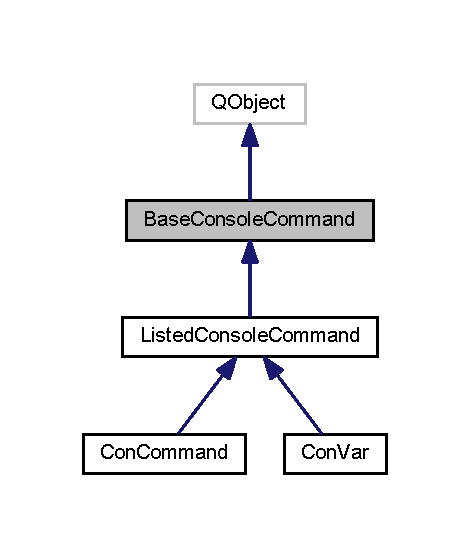
\includegraphics[width=225pt]{class_base_console_command__inherit__graph}
\end{center}
\end{figure}


Collaboration diagram for Base\-Console\-Command\-:\nopagebreak
\begin{figure}[H]
\begin{center}
\leavevmode
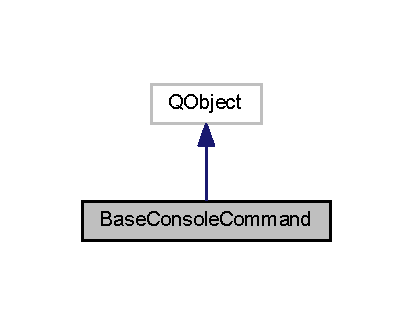
\includegraphics[width=198pt]{class_base_console_command__coll__graph}
\end{center}
\end{figure}
\subsection*{Public Member Functions}
\begin{DoxyCompactItemize}
\item 
\hyperlink{class_base_console_command_af36ba741b2ed473a9fa65921639736d5}{Base\-Console\-Command} (const Q\-String \&\hyperlink{class_base_console_command_a2f21764f46a3864a362eae2e3396e363}{name}, const Q\-String \&desc=\char`\"{}\char`\"{}, N\-Global\-Cmd\-::\-C\-M\-D\-F\-L\-A\-G\-S flags=0, Q\-Object $\ast$parent=0)
\begin{DoxyCompactList}\small\item\em Constructor. \end{DoxyCompactList}\item 
\hypertarget{class_base_console_command_a7d1ca8afdd3549778540595fd9f33881}{virtual \hyperlink{class_base_console_command_a7d1ca8afdd3549778540595fd9f33881}{$\sim$\-Base\-Console\-Command} ()}\label{class_base_console_command_a7d1ca8afdd3549778540595fd9f33881}

\begin{DoxyCompactList}\small\item\em Destructor. \end{DoxyCompactList}\item 
virtual N\-Global\-Cmd\-::\-Cmd\-Ident \hyperlink{class_base_console_command_a8c1fe488f1e24c6bd4891225eb9bb122}{identify} () const 
\begin{DoxyCompactList}\small\item\em Identifies this console command. A \hyperlink{class_base_console_command}{Base\-Console\-Command} object will return C\-I\-Null; other derived commands should return a specific identifier. \end{DoxyCompactList}\item 
Q\-String \hyperlink{class_base_console_command_addf7b841bac36ffc45dd79ec1e697e52}{name} () const 
\begin{DoxyCompactList}\small\item\em Returns the name of the command. \end{DoxyCompactList}\item 
Q\-String \hyperlink{class_base_console_command_a8eaacc83646c4cca95a772a623343988}{description} () const 
\begin{DoxyCompactList}\small\item\em Returns the description of the command. \end{DoxyCompactList}\item 
N\-Global\-Cmd\-::\-C\-M\-D\-F\-L\-A\-G\-S \hyperlink{class_base_console_command_a2e8b8d3a73e0684c7992945fd5d0a216}{flags\-Raw} () const 
\begin{DoxyCompactList}\small\item\em Returns the command's collection of flags. \end{DoxyCompactList}\item 
void \hyperlink{class_base_console_command_ac6ff6169ab06ae43d76d0b3c2e5336ff}{set\-Flags\-Raw} (N\-Global\-Cmd\-::\-C\-M\-D\-F\-L\-A\-G\-S flags)
\begin{DoxyCompactList}\small\item\em Overwrites all flags on the command. \end{DoxyCompactList}\item 
bool \hyperlink{class_base_console_command_a021a4299766424a10f1ec9398c6edb3e}{flag\-Set} (N\-Global\-Cmd\-::\-C\-M\-D\-F\-L\-A\-G\-S flag) const 
\begin{DoxyCompactList}\small\item\em Returns whether a given flag is set. Can test combinations of flags. \end{DoxyCompactList}\item 
void \hyperlink{class_base_console_command_a3046da732d30b1de8b41f51d146b5e46}{set\-Flag} (N\-Global\-Cmd\-::\-C\-M\-D\-F\-L\-A\-G\-S flag)
\begin{DoxyCompactList}\small\item\em Sets the given flag(s) on the command. \end{DoxyCompactList}\item 
void \hyperlink{class_base_console_command_a074b1ecedbef610eaa4a0e9d378f9da9}{remove\-Flag} (N\-Global\-Cmd\-::\-C\-M\-D\-F\-L\-A\-G\-S flag)
\begin{DoxyCompactList}\small\item\em Un-\/sets the given flag(s) from the command. \end{DoxyCompactList}\item 
void \hyperlink{class_base_console_command_a509caa8e6fba5c10e9ff89dd5fb665cf}{toggle\-Flag} (N\-Global\-Cmd\-::\-C\-M\-D\-F\-L\-A\-G\-S flag)
\begin{DoxyCompactList}\small\item\em Toggles the given flag(s) on the command. \end{DoxyCompactList}\end{DoxyCompactItemize}
\subsection*{Properties}
\begin{DoxyCompactItemize}
\item 
\hypertarget{class_base_console_command_a2f21764f46a3864a362eae2e3396e363}{Q\-String \hyperlink{class_base_console_command_a2f21764f46a3864a362eae2e3396e363}{name}}\label{class_base_console_command_a2f21764f46a3864a362eae2e3396e363}

\begin{DoxyCompactList}\small\item\em Name of the command.  name() \end{DoxyCompactList}\item 
\hypertarget{class_base_console_command_afcb44c52f870b7ca902da018c365b758}{Q\-String \hyperlink{class_base_console_command_afcb44c52f870b7ca902da018c365b758}{description}}\label{class_base_console_command_afcb44c52f870b7ca902da018c365b758}

\begin{DoxyCompactList}\small\item\em Description of the command.  description() \end{DoxyCompactList}\item 
\hypertarget{class_base_console_command_af736ebf1192e20424a3b738422cb55dc}{N\-Global\-Cmd\-::\-C\-M\-D\-F\-L\-A\-G\-S \hyperlink{class_base_console_command_af736ebf1192e20424a3b738422cb55dc}{flags\-Raw}}\label{class_base_console_command_af736ebf1192e20424a3b738422cb55dc}

\begin{DoxyCompactList}\small\item\em Raw collection of command flags.  flags\-Raw(), \hyperlink{class_base_console_command_ac6ff6169ab06ae43d76d0b3c2e5336ff}{set\-Flags\-Raw()} \end{DoxyCompactList}\end{DoxyCompactItemize}


\subsection{Detailed Description}
Class defining properties common to all console commands. 

A \hyperlink{class_base_console_command}{Base\-Console\-Command} contains data referring to the command's name, description, flags and identification. A \hyperlink{class_base_console_command}{Base\-Console\-Command} identifies as N\-Global\-Command\-::\-Cmd\-Ident\-::\-C\-I\-Null. 

\subsection{Constructor \& Destructor Documentation}
\hypertarget{class_base_console_command_af36ba741b2ed473a9fa65921639736d5}{\index{Base\-Console\-Command@{Base\-Console\-Command}!Base\-Console\-Command@{Base\-Console\-Command}}
\index{Base\-Console\-Command@{Base\-Console\-Command}!BaseConsoleCommand@{Base\-Console\-Command}}
\subsubsection[{Base\-Console\-Command}]{\setlength{\rightskip}{0pt plus 5cm}Base\-Console\-Command\-::\-Base\-Console\-Command (
\begin{DoxyParamCaption}
\item[{const Q\-String \&}]{name, }
\item[{const Q\-String \&}]{desc = {\ttfamily \char`\"{}\char`\"{}}, }
\item[{N\-Global\-Cmd\-::\-C\-M\-D\-F\-L\-A\-G\-S}]{flags = {\ttfamily 0}, }
\item[{Q\-Object $\ast$}]{parent = {\ttfamily 0}}
\end{DoxyParamCaption}
)\hspace{0.3cm}{\ttfamily [explicit]}}}\label{class_base_console_command_af36ba741b2ed473a9fa65921639736d5}


Constructor. 


\begin{DoxyParams}{Parameters}
{\em name} & Name of the command. \\
\hline
{\em desc} & Optional description of the command. \\
\hline
{\em flags} & Command flags. \\
\hline
{\em parent} & Parent Q\-Object, if applicable. \\
\hline
\end{DoxyParams}


\subsection{Member Function Documentation}
\hypertarget{class_base_console_command_a8eaacc83646c4cca95a772a623343988}{\index{Base\-Console\-Command@{Base\-Console\-Command}!description@{description}}
\index{description@{description}!BaseConsoleCommand@{Base\-Console\-Command}}
\subsubsection[{description}]{\setlength{\rightskip}{0pt plus 5cm}Q\-String Base\-Console\-Command\-::description (
\begin{DoxyParamCaption}
{}
\end{DoxyParamCaption}
) const}}\label{class_base_console_command_a8eaacc83646c4cca95a772a623343988}


Returns the description of the command. 

\begin{DoxyReturn}{Returns}
Command description, or empty string if no description was set. 
\end{DoxyReturn}
\hypertarget{class_base_console_command_a021a4299766424a10f1ec9398c6edb3e}{\index{Base\-Console\-Command@{Base\-Console\-Command}!flag\-Set@{flag\-Set}}
\index{flag\-Set@{flag\-Set}!BaseConsoleCommand@{Base\-Console\-Command}}
\subsubsection[{flag\-Set}]{\setlength{\rightskip}{0pt plus 5cm}bool Base\-Console\-Command\-::flag\-Set (
\begin{DoxyParamCaption}
\item[{N\-Global\-Cmd\-::\-C\-M\-D\-F\-L\-A\-G\-S}]{flag}
\end{DoxyParamCaption}
) const}}\label{class_base_console_command_a021a4299766424a10f1ec9398c6edb3e}


Returns whether a given flag is set. Can test combinations of flags. 


\begin{DoxyParams}{Parameters}
{\em flag} & Flag(s) to test for. \\
\hline
\end{DoxyParams}
\begin{DoxyReturn}{Returns}
True if flag is set (or in the case of multiple test flags, if all are set), false otherwise. 
\end{DoxyReturn}
\hypertarget{class_base_console_command_a2e8b8d3a73e0684c7992945fd5d0a216}{\index{Base\-Console\-Command@{Base\-Console\-Command}!flags\-Raw@{flags\-Raw}}
\index{flags\-Raw@{flags\-Raw}!BaseConsoleCommand@{Base\-Console\-Command}}
\subsubsection[{flags\-Raw}]{\setlength{\rightskip}{0pt plus 5cm}N\-Global\-Cmd\-::\-C\-M\-D\-F\-L\-A\-G\-S Base\-Console\-Command\-::flags\-Raw (
\begin{DoxyParamCaption}
{}
\end{DoxyParamCaption}
) const}}\label{class_base_console_command_a2e8b8d3a73e0684c7992945fd5d0a216}


Returns the command's collection of flags. 

\begin{DoxyReturn}{Returns}
Flags. 
\end{DoxyReturn}
\hypertarget{class_base_console_command_a8c1fe488f1e24c6bd4891225eb9bb122}{\index{Base\-Console\-Command@{Base\-Console\-Command}!identify@{identify}}
\index{identify@{identify}!BaseConsoleCommand@{Base\-Console\-Command}}
\subsubsection[{identify}]{\setlength{\rightskip}{0pt plus 5cm}N\-Global\-Cmd\-::\-Cmd\-Ident Base\-Console\-Command\-::identify (
\begin{DoxyParamCaption}
{}
\end{DoxyParamCaption}
) const\hspace{0.3cm}{\ttfamily [virtual]}}}\label{class_base_console_command_a8c1fe488f1e24c6bd4891225eb9bb122}


Identifies this console command. A \hyperlink{class_base_console_command}{Base\-Console\-Command} object will return C\-I\-Null; other derived commands should return a specific identifier. 

\begin{DoxyReturn}{Returns}
Identifier for the console command. 
\end{DoxyReturn}


Reimplemented in \hyperlink{class_con_command_ab287443a9615df46739d0c39b096016e}{Con\-Command}, and \hyperlink{class_con_var_a0d2fb6068e6fa0ac6b1655327c453d6b}{Con\-Var}.

\hypertarget{class_base_console_command_addf7b841bac36ffc45dd79ec1e697e52}{\index{Base\-Console\-Command@{Base\-Console\-Command}!name@{name}}
\index{name@{name}!BaseConsoleCommand@{Base\-Console\-Command}}
\subsubsection[{name}]{\setlength{\rightskip}{0pt plus 5cm}Q\-String Base\-Console\-Command\-::name (
\begin{DoxyParamCaption}
{}
\end{DoxyParamCaption}
) const}}\label{class_base_console_command_addf7b841bac36ffc45dd79ec1e697e52}


Returns the name of the command. 

\begin{DoxyReturn}{Returns}
Command name. 
\end{DoxyReturn}
\hypertarget{class_base_console_command_a074b1ecedbef610eaa4a0e9d378f9da9}{\index{Base\-Console\-Command@{Base\-Console\-Command}!remove\-Flag@{remove\-Flag}}
\index{remove\-Flag@{remove\-Flag}!BaseConsoleCommand@{Base\-Console\-Command}}
\subsubsection[{remove\-Flag}]{\setlength{\rightskip}{0pt plus 5cm}void Base\-Console\-Command\-::remove\-Flag (
\begin{DoxyParamCaption}
\item[{N\-Global\-Cmd\-::\-C\-M\-D\-F\-L\-A\-G\-S}]{flag}
\end{DoxyParamCaption}
)}}\label{class_base_console_command_a074b1ecedbef610eaa4a0e9d378f9da9}


Un-\/sets the given flag(s) from the command. 


\begin{DoxyParams}{Parameters}
{\em flag} & Flag(s) to Un-\/set. \\
\hline
\end{DoxyParams}
\hypertarget{class_base_console_command_a3046da732d30b1de8b41f51d146b5e46}{\index{Base\-Console\-Command@{Base\-Console\-Command}!set\-Flag@{set\-Flag}}
\index{set\-Flag@{set\-Flag}!BaseConsoleCommand@{Base\-Console\-Command}}
\subsubsection[{set\-Flag}]{\setlength{\rightskip}{0pt plus 5cm}void Base\-Console\-Command\-::set\-Flag (
\begin{DoxyParamCaption}
\item[{N\-Global\-Cmd\-::\-C\-M\-D\-F\-L\-A\-G\-S}]{flag}
\end{DoxyParamCaption}
)}}\label{class_base_console_command_a3046da732d30b1de8b41f51d146b5e46}


Sets the given flag(s) on the command. 


\begin{DoxyParams}{Parameters}
{\em flag} & Flag(s) to set. \\
\hline
\end{DoxyParams}
\hypertarget{class_base_console_command_ac6ff6169ab06ae43d76d0b3c2e5336ff}{\index{Base\-Console\-Command@{Base\-Console\-Command}!set\-Flags\-Raw@{set\-Flags\-Raw}}
\index{set\-Flags\-Raw@{set\-Flags\-Raw}!BaseConsoleCommand@{Base\-Console\-Command}}
\subsubsection[{set\-Flags\-Raw}]{\setlength{\rightskip}{0pt plus 5cm}void Base\-Console\-Command\-::set\-Flags\-Raw (
\begin{DoxyParamCaption}
\item[{N\-Global\-Cmd\-::\-C\-M\-D\-F\-L\-A\-G\-S}]{flags}
\end{DoxyParamCaption}
)}}\label{class_base_console_command_ac6ff6169ab06ae43d76d0b3c2e5336ff}


Overwrites all flags on the command. 


\begin{DoxyParams}{Parameters}
{\em flags} & Integer containing the exact state of all flags to set. \\
\hline
\end{DoxyParams}
\hypertarget{class_base_console_command_a509caa8e6fba5c10e9ff89dd5fb665cf}{\index{Base\-Console\-Command@{Base\-Console\-Command}!toggle\-Flag@{toggle\-Flag}}
\index{toggle\-Flag@{toggle\-Flag}!BaseConsoleCommand@{Base\-Console\-Command}}
\subsubsection[{toggle\-Flag}]{\setlength{\rightskip}{0pt plus 5cm}void Base\-Console\-Command\-::toggle\-Flag (
\begin{DoxyParamCaption}
\item[{N\-Global\-Cmd\-::\-C\-M\-D\-F\-L\-A\-G\-S}]{flag}
\end{DoxyParamCaption}
)}}\label{class_base_console_command_a509caa8e6fba5c10e9ff89dd5fb665cf}


Toggles the given flag(s) on the command. 


\begin{DoxyParams}{Parameters}
{\em flag} & Flag(s) to toggle. \\
\hline
\end{DoxyParams}


The documentation for this class was generated from the following files\-:\begin{DoxyCompactItemize}
\item 
I\-Console/inc/\hyperlink{baseconsolecommand_8h}{baseconsolecommand.\-h}\item 
I\-Console/src/baseconsolecommand.\-cpp\end{DoxyCompactItemize}

\hypertarget{class_command_entry_box}{\section{Command\-Entry\-Box Class Reference}
\label{class_command_entry_box}\index{Command\-Entry\-Box@{Command\-Entry\-Box}}
}


Manages input of console commands by the user.  




{\ttfamily \#include $<$commandentrybox.\-h$>$}



Inheritance diagram for Command\-Entry\-Box\-:\nopagebreak
\begin{figure}[H]
\begin{center}
\leavevmode
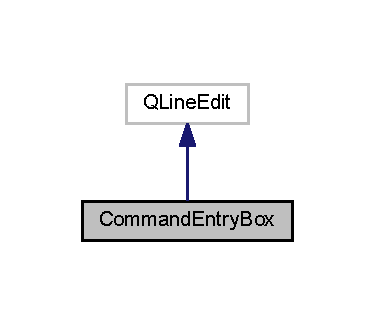
\includegraphics[width=180pt]{class_command_entry_box__inherit__graph}
\end{center}
\end{figure}


Collaboration diagram for Command\-Entry\-Box\-:\nopagebreak
\begin{figure}[H]
\begin{center}
\leavevmode
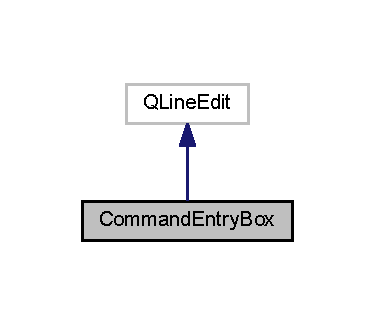
\includegraphics[width=180pt]{class_command_entry_box__coll__graph}
\end{center}
\end{figure}
\subsection*{Public Slots}
\begin{DoxyCompactItemize}
\item 
\hypertarget{class_command_entry_box_a8310199329ce545fefd767066631250b}{void \hyperlink{class_command_entry_box_a8310199329ce545fefd767066631250b}{send\-Command\-String} ()}\label{class_command_entry_box_a8310199329ce545fefd767066631250b}

\begin{DoxyCompactList}\small\item\em Sends the current command string. Results in the command\-String signal being emitted. \end{DoxyCompactList}\item 
\hypertarget{class_command_entry_box_a238530c1dbe9c56b872759b4dec70239}{void \hyperlink{class_command_entry_box_a238530c1dbe9c56b872759b4dec70239}{reposition\-Suggestions} ()}\label{class_command_entry_box_a238530c1dbe9c56b872759b4dec70239}

\begin{DoxyCompactList}\small\item\em Tells the entry box that the suggestion list should be repositioned to the entry box's current position. \end{DoxyCompactList}\item 
\hypertarget{class_command_entry_box_ae40495ddfe607385ba9a0d00f30c5757}{void \hyperlink{class_command_entry_box_ae40495ddfe607385ba9a0d00f30c5757}{move\-Suggestion\-Selection\-Up} ()}\label{class_command_entry_box_ae40495ddfe607385ba9a0d00f30c5757}

\begin{DoxyCompactList}\small\item\em Moves the current selection in the command suggestion box up one entry. \end{DoxyCompactList}\item 
\hypertarget{class_command_entry_box_a4a95a141eba1cc7869fbcf47af3ac972}{void \hyperlink{class_command_entry_box_a4a95a141eba1cc7869fbcf47af3ac972}{choose\-Above\-Suggestion} ()}\label{class_command_entry_box_a4a95a141eba1cc7869fbcf47af3ac972}

\begin{DoxyCompactList}\small\item\em If the suggestion box is present, chooses the entry directly above the current suggestion and inserts the text into the entry box. The suggestion list is not closed. If the suggestion box is not present, moves back one in the command history and inserts the command string into the entry box. \end{DoxyCompactList}\item 
\hypertarget{class_command_entry_box_a306ce6835a28f12b3c7103b01dd7be1a}{void \hyperlink{class_command_entry_box_a306ce6835a28f12b3c7103b01dd7be1a}{move\-Suggestion\-Selection\-Down} ()}\label{class_command_entry_box_a306ce6835a28f12b3c7103b01dd7be1a}

\begin{DoxyCompactList}\small\item\em Moves the current selection in the command suggestion box down one entry. \end{DoxyCompactList}\item 
\hypertarget{class_command_entry_box_a83b4d111d9b5d358752fd91876cd8b16}{void \hyperlink{class_command_entry_box_a83b4d111d9b5d358752fd91876cd8b16}{choose\-Below\-Suggestion} ()}\label{class_command_entry_box_a83b4d111d9b5d358752fd91876cd8b16}

\begin{DoxyCompactList}\small\item\em If the suggestion box is present, chooses the entry directly below the current suggestion and inserts the text into the entry box. The suggestion list is not closed. If the suggestion box is not present, moves forward one in the command history and inserts the command string into the entry box. \end{DoxyCompactList}\item 
\hypertarget{class_command_entry_box_af1af0e911dd16951a7c38c7cdbf18151}{void \hyperlink{class_command_entry_box_af1af0e911dd16951a7c38c7cdbf18151}{complete\-With\-Current\-Suggestion} ()}\label{class_command_entry_box_af1af0e911dd16951a7c38c7cdbf18151}

\begin{DoxyCompactList}\small\item\em Chooses the currently selected command suggestion and insert it into the entry box before closing the suggestion list. \end{DoxyCompactList}\item 
void \hyperlink{class_command_entry_box_a54b2fc4ebce5af818b61b3ade395fe3d}{scroll\-Suggestion\-Selection} (int n)
\begin{DoxyCompactList}\small\item\em Scrolls {\itshape n} entries up or down in the suggestion list and inserts the resulting selection into the entry box. \end{DoxyCompactList}\item 
void \hyperlink{class_command_entry_box_a7d011c6ec9253d4f4c994934d7275567}{process\-For\-Suggestions} (const Q\-String \&str)
\begin{DoxyCompactList}\small\item\em Processes the current partial command string and requests suggestions if required. \end{DoxyCompactList}\item 
void \hyperlink{class_command_entry_box_a922f73bd213ce52fb728f7459ac43a1c}{complete\-List\-Item} (Q\-List\-Widget\-Item $\ast$item)
\begin{DoxyCompactList}\small\item\em Inserts the command held by the list item into the entry box. \end{DoxyCompactList}\item 
\hypertarget{class_command_entry_box_a3d5fbb81f6400d1b827607feb1153606}{void \hyperlink{class_command_entry_box_a3d5fbb81f6400d1b827607feb1153606}{clear\-Command\-History} ()}\label{class_command_entry_box_a3d5fbb81f6400d1b827607feb1153606}

\begin{DoxyCompactList}\small\item\em Clears the command history buffer. \end{DoxyCompactList}\end{DoxyCompactItemize}
\subsection*{Signals}
\begin{DoxyCompactItemize}
\item 
void \hyperlink{class_command_entry_box_ac3a24b4e68ffd823d14c37b212290fa3}{command\-String} (const Q\-String \&command)
\begin{DoxyCompactList}\small\item\em Emitted when the user executes the command string they have been entering. \end{DoxyCompactList}\item 
void \hyperlink{class_command_entry_box_a926587c4199c009a85daec24624968f4}{get\-Suggestions} (const Q\-String \&prefix, Q\-List$<$ \hyperlink{class_command_interpreter_acef7360cdc3e98c4d35ec54954c4e39c}{Command\-Interpreter\-::\-Command\-Ident\-Pair} $>$ \&list, int count=-\/1)
\begin{DoxyCompactList}\small\item\em Emitted when the entry box requests that its command suggestion list be filled with suggestions for the current command string prefix. \end{DoxyCompactList}\item 
\hypertarget{class_command_entry_box_a2808bdf010ef238092b3cc3c050cbfdb}{void \hyperlink{class_command_entry_box_a2808bdf010ef238092b3cc3c050cbfdb}{tab\-Pressed} ()}\label{class_command_entry_box_a2808bdf010ef238092b3cc3c050cbfdb}

\begin{DoxyCompactList}\small\item\em Tab has been pressed while the entry box has focus. \end{DoxyCompactList}\item 
\hypertarget{class_command_entry_box_a5759602d5713c0f2f7fb9f68c5f7c507}{void \hyperlink{class_command_entry_box_a5759602d5713c0f2f7fb9f68c5f7c507}{up\-Arrow\-Pressed} ()}\label{class_command_entry_box_a5759602d5713c0f2f7fb9f68c5f7c507}

\begin{DoxyCompactList}\small\item\em Up arrow has been pressed while the entry box has focus. \end{DoxyCompactList}\item 
\hypertarget{class_command_entry_box_abd5ca1d5f1eb6d5d5c1b5174d9cdf5fb}{void \hyperlink{class_command_entry_box_abd5ca1d5f1eb6d5d5c1b5174d9cdf5fb}{down\-Arrow\-Pressed} ()}\label{class_command_entry_box_abd5ca1d5f1eb6d5d5c1b5174d9cdf5fb}

\begin{DoxyCompactList}\small\item\em Down arrow has been pressed while the entry box has focus. \end{DoxyCompactList}\item 
void \hyperlink{class_command_entry_box_a8399e5aa78c5841dd0c60f7a5285410b}{mouse\-Wheel} (int delta\-Degrees)
\begin{DoxyCompactList}\small\item\em The user moved the mouse wheel while the entry box has focus. \end{DoxyCompactList}\item 
\hypertarget{class_command_entry_box_ac13c5c8a5aa22fd0fb264010ee271ea8}{void \hyperlink{class_command_entry_box_ac13c5c8a5aa22fd0fb264010ee271ea8}{icon\-Con\-Command\-Changed} ()}\label{class_command_entry_box_ac13c5c8a5aa22fd0fb264010ee271ea8}

\begin{DoxyCompactList}\small\item\em The console command icon path has been changed. \end{DoxyCompactList}\item 
\hypertarget{class_command_entry_box_a971a6587e79b6420a09963c09daa61a4}{void \hyperlink{class_command_entry_box_a971a6587e79b6420a09963c09daa61a4}{icon\-Con\-Var\-Changed} ()}\label{class_command_entry_box_a971a6587e79b6420a09963c09daa61a4}

\begin{DoxyCompactList}\small\item\em The console variable icon path has been changed. \end{DoxyCompactList}\item 
\hypertarget{class_command_entry_box_a89f2868238ec30998795c227fbaab143}{void \hyperlink{class_command_entry_box_a89f2868238ec30998795c227fbaab143}{command\-History\-Size\-Changed} ()}\label{class_command_entry_box_a89f2868238ec30998795c227fbaab143}

\begin{DoxyCompactList}\small\item\em The command history buffer size has been changed. \end{DoxyCompactList}\end{DoxyCompactItemize}
\subsection*{Public Member Functions}
\begin{DoxyCompactItemize}
\item 
\hyperlink{class_command_entry_box_a75c9cb2fee4e0034bc114222fa890e3b}{Command\-Entry\-Box} (Q\-Widget $\ast$parent=0)
\begin{DoxyCompactList}\small\item\em Constructor. \end{DoxyCompactList}\item 
\hypertarget{class_command_entry_box_a66f323c649a34cc167f124069aa5de53}{virtual \hyperlink{class_command_entry_box_a66f323c649a34cc167f124069aa5de53}{$\sim$\-Command\-Entry\-Box} ()}\label{class_command_entry_box_a66f323c649a34cc167f124069aa5de53}

\begin{DoxyCompactList}\small\item\em Destructor. \end{DoxyCompactList}\item 
const \hyperlink{class_command_suggestion_list}{Command\-Suggestion\-List} $\ast$ \hyperlink{class_command_entry_box_ae00fdd5b4cbf8fc825e5333f3ae47dad}{get\-Suggestion\-List} () const 
\begin{DoxyCompactList}\small\item\em Returns the command suggestion list belonging to this entry box. \end{DoxyCompactList}\item 
Q\-String \hyperlink{class_command_entry_box_a4ff50a0239789c705b15a395cd1d3a68}{icon\-Con\-Command} () const 
\begin{DoxyCompactList}\small\item\em Returns the file name and path of the icon displayed in the suggestion box for a console command entry. Path is relative to the application directory. \end{DoxyCompactList}\item 
void \hyperlink{class_command_entry_box_a5fc40503d8f9b6bf8faddc42ff6663bb}{set\-Icon\-Con\-Command} (Q\-String icon)
\begin{DoxyCompactList}\small\item\em Sets the file name and path of the icon to display in the suggestion box next to a console command entry. Path should be relative to the application directory. \end{DoxyCompactList}\item 
\hypertarget{class_command_entry_box_a9807265bf78369d6dfbc8210aa39c562}{void \hyperlink{class_command_entry_box_a9807265bf78369d6dfbc8210aa39c562}{reset\-Icon\-Con\-Command} ()}\label{class_command_entry_box_a9807265bf78369d6dfbc8210aa39c562}

\begin{DoxyCompactList}\small\item\em Resets (blanks) the icon path string for the console command list entry icon. \end{DoxyCompactList}\item 
Q\-String \hyperlink{class_command_entry_box_ac7147c8f991326bcf6339d60220a4f58}{icon\-Con\-Var} () const 
\begin{DoxyCompactList}\small\item\em Returns the file name and path of the icon displayed in the suggestion box for a console variable entry. Path is relative to the application directory. \end{DoxyCompactList}\item 
void \hyperlink{class_command_entry_box_a9e4387c47cb2de50da44360110d9e59a}{set\-Icon\-Con\-Var} (Q\-String icon)
\begin{DoxyCompactList}\small\item\em Sets the file name and path of the icon to display in the suggestion box next to a console variable entry. Path should be relative to the application directory. \end{DoxyCompactList}\item 
\hypertarget{class_command_entry_box_a85705eaae1055472de96c07142cf56af}{void \hyperlink{class_command_entry_box_a85705eaae1055472de96c07142cf56af}{reset\-Icon\-Con\-Var} ()}\label{class_command_entry_box_a85705eaae1055472de96c07142cf56af}

\begin{DoxyCompactList}\small\item\em Resets (blanks) the icon path string for the console command list entry icon. \end{DoxyCompactList}\item 
int \hyperlink{class_command_entry_box_a1c7d6384d3009e3685fb45f238c8a279}{command\-History\-Size} () const 
\begin{DoxyCompactList}\small\item\em Returns the current size of the command history buffer -\/ how many previously typed commands the entry box will remember. \end{DoxyCompactList}\item 
void \hyperlink{class_command_entry_box_a96513e1f106fbf5e734c6a4ff7a26e2d}{set\-Command\-History\-Size} (int size)
\begin{DoxyCompactList}\small\item\em Sets the size of the command history buffer. \end{DoxyCompactList}\item 
void \hyperlink{class_command_entry_box_ad81eaeb870ed56bc231cd962d527b520}{reset\-Command\-History\-Size} ()
\begin{DoxyCompactList}\small\item\em Resets the command history buffer to the default size. \end{DoxyCompactList}\end{DoxyCompactItemize}
\subsection*{Static Public Attributes}
\begin{DoxyCompactItemize}
\item 
\hypertarget{class_command_entry_box_afccb0e6456f6aa1264e5db11fdf1ca4e}{static const Q\-String \hyperlink{class_command_entry_box_afccb0e6456f6aa1264e5db11fdf1ca4e}{L\-I\-\_\-\-N\-A\-M\-E\-\_\-\-C\-O\-M\-M\-A\-N\-D} = \char`\"{}Command\-List\-Item\char`\"{}}\label{class_command_entry_box_afccb0e6456f6aa1264e5db11fdf1ca4e}

\begin{DoxyCompactList}\small\item\em Identifying name of a command suggestion list item which contains the name of a console command. \end{DoxyCompactList}\item 
\hypertarget{class_command_entry_box_a5301bf4e9f267a5d773ddcc087ae6d83}{static const Q\-String \hyperlink{class_command_entry_box_a5301bf4e9f267a5d773ddcc087ae6d83}{L\-I\-\_\-\-N\-A\-M\-E\-\_\-\-V\-A\-R\-I\-A\-B\-L\-E} = \char`\"{}Variable\-List\-Item\char`\"{}}\label{class_command_entry_box_a5301bf4e9f267a5d773ddcc087ae6d83}

\begin{DoxyCompactList}\small\item\em Identifying name of a command suggestion list item which contains the name of a console variable. \end{DoxyCompactList}\item 
\hypertarget{class_command_entry_box_a52a1a304da91b347e879e095cf5eab67}{static const int \hyperlink{class_command_entry_box_a52a1a304da91b347e879e095cf5eab67}{D\-E\-F\-A\-U\-L\-T\-\_\-\-C\-O\-M\-M\-A\-N\-D\-\_\-\-H\-I\-S\-T\-O\-R\-Y\-\_\-\-S\-I\-Z\-E} = 32}\label{class_command_entry_box_a52a1a304da91b347e879e095cf5eab67}

\begin{DoxyCompactList}\small\item\em Default size of the command history buffer (how many previously typed commands this entry box will remember. \end{DoxyCompactList}\end{DoxyCompactItemize}
\subsection*{Properties}
\begin{DoxyCompactItemize}
\item 
Q\-String \hyperlink{class_command_entry_box_ac53924ba07f11bab5b255af0625ffbd6}{icon\-Con\-Command}
\begin{DoxyCompactList}\small\item\em Path to icon to display for a \hyperlink{class_con_command}{Con\-Command} suggestion entry. \end{DoxyCompactList}\item 
Q\-String \hyperlink{class_command_entry_box_ad069b345272bd9d2fe43266ac5ead588}{icon\-Con\-Var}
\begin{DoxyCompactList}\small\item\em Path to icon to display for a \hyperlink{class_con_var}{Con\-Var} suggestion entry. \end{DoxyCompactList}\item 
int \hyperlink{class_command_entry_box_ad659bb8ce66cbf009d51d31ca2589207}{command\-History\-Size}
\begin{DoxyCompactList}\small\item\em Size of the command history buffer. \end{DoxyCompactList}\end{DoxyCompactItemize}


\subsection{Detailed Description}
Manages input of console commands by the user. 

The \hyperlink{class_command_entry_box}{Command\-Entry\-Box} is a specialised Q\-Line\-Edit which owns a popup suggestion window. Command strings are parsed as the user types them and the get\-Suggestions signal is emitted whenever command suggestions are required by the entry box. The command\-String signal is also emitted when the user's command should be sent to a \hyperlink{class_command_interpreter}{Command\-Interpreter} for execution. 

\subsection{Constructor \& Destructor Documentation}
\hypertarget{class_command_entry_box_a75c9cb2fee4e0034bc114222fa890e3b}{\index{Command\-Entry\-Box@{Command\-Entry\-Box}!Command\-Entry\-Box@{Command\-Entry\-Box}}
\index{Command\-Entry\-Box@{Command\-Entry\-Box}!CommandEntryBox@{Command\-Entry\-Box}}
\subsubsection[{Command\-Entry\-Box}]{\setlength{\rightskip}{0pt plus 5cm}Command\-Entry\-Box\-::\-Command\-Entry\-Box (
\begin{DoxyParamCaption}
\item[{Q\-Widget $\ast$}]{parent = {\ttfamily 0}}
\end{DoxyParamCaption}
)\hspace{0.3cm}{\ttfamily [explicit]}}}\label{class_command_entry_box_a75c9cb2fee4e0034bc114222fa890e3b}


Constructor. 


\begin{DoxyParams}{Parameters}
{\em parent} & Q\-Widget parent, if applicable. \\
\hline
\end{DoxyParams}


\subsection{Member Function Documentation}
\hypertarget{class_command_entry_box_a1c7d6384d3009e3685fb45f238c8a279}{\index{Command\-Entry\-Box@{Command\-Entry\-Box}!command\-History\-Size@{command\-History\-Size}}
\index{command\-History\-Size@{command\-History\-Size}!CommandEntryBox@{Command\-Entry\-Box}}
\subsubsection[{command\-History\-Size}]{\setlength{\rightskip}{0pt plus 5cm}int Command\-Entry\-Box\-::command\-History\-Size (
\begin{DoxyParamCaption}
{}
\end{DoxyParamCaption}
) const}}\label{class_command_entry_box_a1c7d6384d3009e3685fb45f238c8a279}


Returns the current size of the command history buffer -\/ how many previously typed commands the entry box will remember. 

\begin{DoxyReturn}{Returns}
Size of command history buffer. 
\end{DoxyReturn}
\hypertarget{class_command_entry_box_ac3a24b4e68ffd823d14c37b212290fa3}{\index{Command\-Entry\-Box@{Command\-Entry\-Box}!command\-String@{command\-String}}
\index{command\-String@{command\-String}!CommandEntryBox@{Command\-Entry\-Box}}
\subsubsection[{command\-String}]{\setlength{\rightskip}{0pt plus 5cm}void Command\-Entry\-Box\-::command\-String (
\begin{DoxyParamCaption}
\item[{const Q\-String \&}]{command}
\end{DoxyParamCaption}
)\hspace{0.3cm}{\ttfamily [signal]}}}\label{class_command_entry_box_ac3a24b4e68ffd823d14c37b212290fa3}


Emitted when the user executes the command string they have been entering. 


\begin{DoxyParams}{Parameters}
{\em command} & Command string the user entered. \\
\hline
\end{DoxyParams}
\hypertarget{class_command_entry_box_a922f73bd213ce52fb728f7459ac43a1c}{\index{Command\-Entry\-Box@{Command\-Entry\-Box}!complete\-List\-Item@{complete\-List\-Item}}
\index{complete\-List\-Item@{complete\-List\-Item}!CommandEntryBox@{Command\-Entry\-Box}}
\subsubsection[{complete\-List\-Item}]{\setlength{\rightskip}{0pt plus 5cm}void Command\-Entry\-Box\-::complete\-List\-Item (
\begin{DoxyParamCaption}
\item[{Q\-List\-Widget\-Item $\ast$}]{item}
\end{DoxyParamCaption}
)\hspace{0.3cm}{\ttfamily [slot]}}}\label{class_command_entry_box_a922f73bd213ce52fb728f7459ac43a1c}


Inserts the command held by the list item into the entry box. 


\begin{DoxyParams}{Parameters}
{\em item} & Item holding the command to insert. \\
\hline
\end{DoxyParams}
\hypertarget{class_command_entry_box_ae00fdd5b4cbf8fc825e5333f3ae47dad}{\index{Command\-Entry\-Box@{Command\-Entry\-Box}!get\-Suggestion\-List@{get\-Suggestion\-List}}
\index{get\-Suggestion\-List@{get\-Suggestion\-List}!CommandEntryBox@{Command\-Entry\-Box}}
\subsubsection[{get\-Suggestion\-List}]{\setlength{\rightskip}{0pt plus 5cm}const {\bf Command\-Suggestion\-List} $\ast$ Command\-Entry\-Box\-::get\-Suggestion\-List (
\begin{DoxyParamCaption}
{}
\end{DoxyParamCaption}
) const}}\label{class_command_entry_box_ae00fdd5b4cbf8fc825e5333f3ae47dad}


Returns the command suggestion list belonging to this entry box. 

\begin{DoxyReturn}{Returns}
Suggestion list for this entry box. 
\end{DoxyReturn}
\hypertarget{class_command_entry_box_a926587c4199c009a85daec24624968f4}{\index{Command\-Entry\-Box@{Command\-Entry\-Box}!get\-Suggestions@{get\-Suggestions}}
\index{get\-Suggestions@{get\-Suggestions}!CommandEntryBox@{Command\-Entry\-Box}}
\subsubsection[{get\-Suggestions}]{\setlength{\rightskip}{0pt plus 5cm}void Command\-Entry\-Box\-::get\-Suggestions (
\begin{DoxyParamCaption}
\item[{const Q\-String \&}]{prefix, }
\item[{Q\-List$<$ {\bf Command\-Interpreter\-::\-Command\-Ident\-Pair} $>$ \&}]{list, }
\item[{int}]{count = {\ttfamily -\/1}}
\end{DoxyParamCaption}
)\hspace{0.3cm}{\ttfamily [signal]}}}\label{class_command_entry_box_a926587c4199c009a85daec24624968f4}


Emitted when the entry box requests that its command suggestion list be filled with suggestions for the current command string prefix. 


\begin{DoxyParams}{Parameters}
{\em prefix} & The string the user has entered so far, to be matched against the beginning of pre-\/existing commands. \\
\hline
{\em list} & List to fill with suggestion entries. \\
\hline
{\em count} & Maximum number of suggestions desired, or -\/1 if no limit. \\
\hline
\end{DoxyParams}
\hypertarget{class_command_entry_box_a4ff50a0239789c705b15a395cd1d3a68}{\index{Command\-Entry\-Box@{Command\-Entry\-Box}!icon\-Con\-Command@{icon\-Con\-Command}}
\index{icon\-Con\-Command@{icon\-Con\-Command}!CommandEntryBox@{Command\-Entry\-Box}}
\subsubsection[{icon\-Con\-Command}]{\setlength{\rightskip}{0pt plus 5cm}Q\-String Command\-Entry\-Box\-::icon\-Con\-Command (
\begin{DoxyParamCaption}
{}
\end{DoxyParamCaption}
) const}}\label{class_command_entry_box_a4ff50a0239789c705b15a395cd1d3a68}


Returns the file name and path of the icon displayed in the suggestion box for a console command entry. Path is relative to the application directory. 

\begin{DoxyReturn}{Returns}
Path to the current icon displayed, or an empty string if no icon should be displayed. 
\end{DoxyReturn}
\hypertarget{class_command_entry_box_ac7147c8f991326bcf6339d60220a4f58}{\index{Command\-Entry\-Box@{Command\-Entry\-Box}!icon\-Con\-Var@{icon\-Con\-Var}}
\index{icon\-Con\-Var@{icon\-Con\-Var}!CommandEntryBox@{Command\-Entry\-Box}}
\subsubsection[{icon\-Con\-Var}]{\setlength{\rightskip}{0pt plus 5cm}Q\-String Command\-Entry\-Box\-::icon\-Con\-Var (
\begin{DoxyParamCaption}
{}
\end{DoxyParamCaption}
) const}}\label{class_command_entry_box_ac7147c8f991326bcf6339d60220a4f58}


Returns the file name and path of the icon displayed in the suggestion box for a console variable entry. Path is relative to the application directory. 

\begin{DoxyReturn}{Returns}
Path to the current icon displayed, or an empty string if no icon should be displayed. 
\end{DoxyReturn}
\hypertarget{class_command_entry_box_a8399e5aa78c5841dd0c60f7a5285410b}{\index{Command\-Entry\-Box@{Command\-Entry\-Box}!mouse\-Wheel@{mouse\-Wheel}}
\index{mouse\-Wheel@{mouse\-Wheel}!CommandEntryBox@{Command\-Entry\-Box}}
\subsubsection[{mouse\-Wheel}]{\setlength{\rightskip}{0pt plus 5cm}void Command\-Entry\-Box\-::mouse\-Wheel (
\begin{DoxyParamCaption}
\item[{int}]{delta\-Degrees}
\end{DoxyParamCaption}
)\hspace{0.3cm}{\ttfamily [signal]}}}\label{class_command_entry_box_a8399e5aa78c5841dd0c60f7a5285410b}


The user moved the mouse wheel while the entry box has focus. 


\begin{DoxyParams}{Parameters}
{\em delta\-Degrees} & Number of degrees the mouse wheel was moved. \\
\hline
\end{DoxyParams}
\hypertarget{class_command_entry_box_a7d011c6ec9253d4f4c994934d7275567}{\index{Command\-Entry\-Box@{Command\-Entry\-Box}!process\-For\-Suggestions@{process\-For\-Suggestions}}
\index{process\-For\-Suggestions@{process\-For\-Suggestions}!CommandEntryBox@{Command\-Entry\-Box}}
\subsubsection[{process\-For\-Suggestions}]{\setlength{\rightskip}{0pt plus 5cm}void Command\-Entry\-Box\-::process\-For\-Suggestions (
\begin{DoxyParamCaption}
\item[{const Q\-String \&}]{str}
\end{DoxyParamCaption}
)\hspace{0.3cm}{\ttfamily [slot]}}}\label{class_command_entry_box_a7d011c6ec9253d4f4c994934d7275567}


Processes the current partial command string and requests suggestions if required. 


\begin{DoxyParams}{Parameters}
{\em str} & Command string, possibly incomplete, to process. \\
\hline
\end{DoxyParams}
\hypertarget{class_command_entry_box_ad81eaeb870ed56bc231cd962d527b520}{\index{Command\-Entry\-Box@{Command\-Entry\-Box}!reset\-Command\-History\-Size@{reset\-Command\-History\-Size}}
\index{reset\-Command\-History\-Size@{reset\-Command\-History\-Size}!CommandEntryBox@{Command\-Entry\-Box}}
\subsubsection[{reset\-Command\-History\-Size}]{\setlength{\rightskip}{0pt plus 5cm}void Command\-Entry\-Box\-::reset\-Command\-History\-Size (
\begin{DoxyParamCaption}
{}
\end{DoxyParamCaption}
)}}\label{class_command_entry_box_ad81eaeb870ed56bc231cd962d527b520}


Resets the command history buffer to the default size. 

\begin{DoxyNote}{Note}
Older commands will be removed from the history if they fall outside the new buffer size. 
\end{DoxyNote}
\hypertarget{class_command_entry_box_a54b2fc4ebce5af818b61b3ade395fe3d}{\index{Command\-Entry\-Box@{Command\-Entry\-Box}!scroll\-Suggestion\-Selection@{scroll\-Suggestion\-Selection}}
\index{scroll\-Suggestion\-Selection@{scroll\-Suggestion\-Selection}!CommandEntryBox@{Command\-Entry\-Box}}
\subsubsection[{scroll\-Suggestion\-Selection}]{\setlength{\rightskip}{0pt plus 5cm}void Command\-Entry\-Box\-::scroll\-Suggestion\-Selection (
\begin{DoxyParamCaption}
\item[{int}]{n}
\end{DoxyParamCaption}
)\hspace{0.3cm}{\ttfamily [slot]}}}\label{class_command_entry_box_a54b2fc4ebce5af818b61b3ade395fe3d}


Scrolls {\itshape n} entries up or down in the suggestion list and inserts the resulting selection into the entry box. 


\begin{DoxyParams}{Parameters}
{\em n} & Number of entries to scroll. Positive values scroll up, negative values scroll down. \\
\hline
\end{DoxyParams}
\hypertarget{class_command_entry_box_a96513e1f106fbf5e734c6a4ff7a26e2d}{\index{Command\-Entry\-Box@{Command\-Entry\-Box}!set\-Command\-History\-Size@{set\-Command\-History\-Size}}
\index{set\-Command\-History\-Size@{set\-Command\-History\-Size}!CommandEntryBox@{Command\-Entry\-Box}}
\subsubsection[{set\-Command\-History\-Size}]{\setlength{\rightskip}{0pt plus 5cm}void Command\-Entry\-Box\-::set\-Command\-History\-Size (
\begin{DoxyParamCaption}
\item[{int}]{size}
\end{DoxyParamCaption}
)}}\label{class_command_entry_box_a96513e1f106fbf5e734c6a4ff7a26e2d}


Sets the size of the command history buffer. 

\begin{DoxyNote}{Note}
Older commands will be removed from the history if they fall outside the new buffer size. 
\end{DoxyNote}

\begin{DoxyParams}{Parameters}
{\em size} & Size to set. \\
\hline
\end{DoxyParams}
\hypertarget{class_command_entry_box_a5fc40503d8f9b6bf8faddc42ff6663bb}{\index{Command\-Entry\-Box@{Command\-Entry\-Box}!set\-Icon\-Con\-Command@{set\-Icon\-Con\-Command}}
\index{set\-Icon\-Con\-Command@{set\-Icon\-Con\-Command}!CommandEntryBox@{Command\-Entry\-Box}}
\subsubsection[{set\-Icon\-Con\-Command}]{\setlength{\rightskip}{0pt plus 5cm}void Command\-Entry\-Box\-::set\-Icon\-Con\-Command (
\begin{DoxyParamCaption}
\item[{Q\-String}]{icon}
\end{DoxyParamCaption}
)}}\label{class_command_entry_box_a5fc40503d8f9b6bf8faddc42ff6663bb}


Sets the file name and path of the icon to display in the suggestion box next to a console command entry. Path should be relative to the application directory. 


\begin{DoxyParams}{Parameters}
{\em icon} & Path to icon file, including extension. \\
\hline
\end{DoxyParams}
\hypertarget{class_command_entry_box_a9e4387c47cb2de50da44360110d9e59a}{\index{Command\-Entry\-Box@{Command\-Entry\-Box}!set\-Icon\-Con\-Var@{set\-Icon\-Con\-Var}}
\index{set\-Icon\-Con\-Var@{set\-Icon\-Con\-Var}!CommandEntryBox@{Command\-Entry\-Box}}
\subsubsection[{set\-Icon\-Con\-Var}]{\setlength{\rightskip}{0pt plus 5cm}void Command\-Entry\-Box\-::set\-Icon\-Con\-Var (
\begin{DoxyParamCaption}
\item[{Q\-String}]{icon}
\end{DoxyParamCaption}
)}}\label{class_command_entry_box_a9e4387c47cb2de50da44360110d9e59a}


Sets the file name and path of the icon to display in the suggestion box next to a console variable entry. Path should be relative to the application directory. 


\begin{DoxyParams}{Parameters}
{\em icon} & Path to icon file, including extension. \\
\hline
\end{DoxyParams}


\subsection{Property Documentation}
\hypertarget{class_command_entry_box_ad659bb8ce66cbf009d51d31ca2589207}{\index{Command\-Entry\-Box@{Command\-Entry\-Box}!command\-History\-Size@{command\-History\-Size}}
\index{command\-History\-Size@{command\-History\-Size}!CommandEntryBox@{Command\-Entry\-Box}}
\subsubsection[{command\-History\-Size}]{\setlength{\rightskip}{0pt plus 5cm}int Command\-Entry\-Box\-::command\-History\-Size\hspace{0.3cm}{\ttfamily [read]}, {\ttfamily [write]}}}\label{class_command_entry_box_ad659bb8ce66cbf009d51d31ca2589207}


Size of the command history buffer. 

\begin{DoxyParagraph}{Accessors\-:}
\hyperlink{class_command_entry_box_ad659bb8ce66cbf009d51d31ca2589207}{command\-History\-Size()}, \hyperlink{class_command_entry_box_a96513e1f106fbf5e734c6a4ff7a26e2d}{set\-Command\-History\-Size()}, \hyperlink{class_command_entry_box_ad81eaeb870ed56bc231cd962d527b520}{reset\-Command\-History\-Size()}, \hyperlink{class_command_entry_box_a89f2868238ec30998795c227fbaab143}{command\-History\-Size\-Changed()} 
\end{DoxyParagraph}
\hypertarget{class_command_entry_box_ac53924ba07f11bab5b255af0625ffbd6}{\index{Command\-Entry\-Box@{Command\-Entry\-Box}!icon\-Con\-Command@{icon\-Con\-Command}}
\index{icon\-Con\-Command@{icon\-Con\-Command}!CommandEntryBox@{Command\-Entry\-Box}}
\subsubsection[{icon\-Con\-Command}]{\setlength{\rightskip}{0pt plus 5cm}Q\-String Command\-Entry\-Box\-::icon\-Con\-Command\hspace{0.3cm}{\ttfamily [read]}, {\ttfamily [write]}}}\label{class_command_entry_box_ac53924ba07f11bab5b255af0625ffbd6}


Path to icon to display for a \hyperlink{class_con_command}{Con\-Command} suggestion entry. 

\begin{DoxyParagraph}{Accessors\-:}
\hyperlink{class_command_entry_box_ac53924ba07f11bab5b255af0625ffbd6}{icon\-Con\-Command()}, \hyperlink{class_command_entry_box_a5fc40503d8f9b6bf8faddc42ff6663bb}{set\-Icon\-Con\-Command()}, \hyperlink{class_command_entry_box_a9807265bf78369d6dfbc8210aa39c562}{reset\-Icon\-Con\-Command()}, \hyperlink{class_command_entry_box_ac13c5c8a5aa22fd0fb264010ee271ea8}{icon\-Con\-Command\-Changed()} 
\end{DoxyParagraph}
\hypertarget{class_command_entry_box_ad069b345272bd9d2fe43266ac5ead588}{\index{Command\-Entry\-Box@{Command\-Entry\-Box}!icon\-Con\-Var@{icon\-Con\-Var}}
\index{icon\-Con\-Var@{icon\-Con\-Var}!CommandEntryBox@{Command\-Entry\-Box}}
\subsubsection[{icon\-Con\-Var}]{\setlength{\rightskip}{0pt plus 5cm}Q\-String Command\-Entry\-Box\-::icon\-Con\-Var\hspace{0.3cm}{\ttfamily [read]}, {\ttfamily [write]}}}\label{class_command_entry_box_ad069b345272bd9d2fe43266ac5ead588}


Path to icon to display for a \hyperlink{class_con_var}{Con\-Var} suggestion entry. 

\begin{DoxyParagraph}{Accessors\-:}
\hyperlink{class_command_entry_box_ad069b345272bd9d2fe43266ac5ead588}{icon\-Con\-Var()}, \hyperlink{class_command_entry_box_a9e4387c47cb2de50da44360110d9e59a}{set\-Icon\-Con\-Var()}, \hyperlink{class_command_entry_box_a85705eaae1055472de96c07142cf56af}{reset\-Icon\-Con\-Var()}, \hyperlink{class_command_entry_box_a971a6587e79b6420a09963c09daa61a4}{icon\-Con\-Var\-Changed()} 
\end{DoxyParagraph}


The documentation for this class was generated from the following files\-:\begin{DoxyCompactItemize}
\item 
I\-Console/inc/\hyperlink{commandentrybox_8h}{commandentrybox.\-h}\item 
I\-Console/src/commandentrybox.\-cpp\end{DoxyCompactItemize}

\hypertarget{class_command_interpreter}{\section{Command\-Interpreter Class Reference}
\label{class_command_interpreter}\index{Command\-Interpreter@{Command\-Interpreter}}
}


Handles parsing strings of user input and executing the relevant commands.  




{\ttfamily \#include $<$commandinterpreter.\-h$>$}



Inheritance diagram for Command\-Interpreter\-:\nopagebreak
\begin{figure}[H]
\begin{center}
\leavevmode
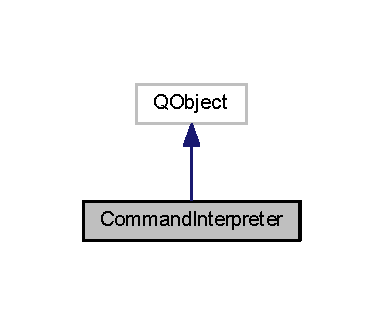
\includegraphics[width=184pt]{class_command_interpreter__inherit__graph}
\end{center}
\end{figure}


Collaboration diagram for Command\-Interpreter\-:\nopagebreak
\begin{figure}[H]
\begin{center}
\leavevmode
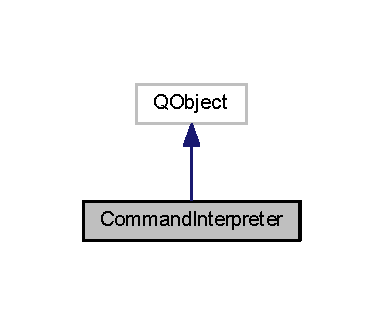
\includegraphics[width=184pt]{class_command_interpreter__coll__graph}
\end{center}
\end{figure}
\subsection*{Public Types}
\begin{DoxyCompactItemize}
\item 
\hypertarget{class_command_interpreter_ac3d555ea1cd2452a773a7d9910c0a7a2}{typedef Q\-Pair$<$ Q\-String, \\*
Q\-String\-List $>$ \hyperlink{class_command_interpreter_ac3d555ea1cd2452a773a7d9910c0a7a2}{Command\-Entry\-Pair}}\label{class_command_interpreter_ac3d555ea1cd2452a773a7d9910c0a7a2}

\begin{DoxyCompactList}\small\item\em Typedef for a pair containing a string and string list. The string corresponds to a command name and the string list to its arguments. \end{DoxyCompactList}\item 
\hypertarget{class_command_interpreter_ab3e2b529b3b064432271873542973cd0}{typedef Q\-List$<$ \hyperlink{class_command_interpreter_ac3d555ea1cd2452a773a7d9910c0a7a2}{Command\-Entry\-Pair} $>$ \hyperlink{class_command_interpreter_ab3e2b529b3b064432271873542973cd0}{Command\-Entry\-Pipe\-List}}\label{class_command_interpreter_ab3e2b529b3b064432271873542973cd0}

\begin{DoxyCompactList}\small\item\em Typedef for a list of command entry pairs. Each command's output is piped into the input of the next command. \end{DoxyCompactList}\item 
\hypertarget{class_command_interpreter_a8b935bf4840835a8ab5f99756268d113}{typedef Q\-List\\*
$<$ \hyperlink{class_command_interpreter_ab3e2b529b3b064432271873542973cd0}{Command\-Entry\-Pipe\-List} $>$ \hyperlink{class_command_interpreter_a8b935bf4840835a8ab5f99756268d113}{Command\-Entry\-List}}\label{class_command_interpreter_a8b935bf4840835a8ab5f99756268d113}

\begin{DoxyCompactList}\small\item\em Typedef for a list of command entry pipe lists. Each pipe list is executed sequentially. \end{DoxyCompactList}\item 
\hypertarget{class_command_interpreter_acef7360cdc3e98c4d35ec54954c4e39c}{typedef Q\-Pair\\*
$<$ N\-Global\-Cmd\-::\-Cmd\-Ident, \\*
Q\-String $>$ \hyperlink{class_command_interpreter_acef7360cdc3e98c4d35ec54954c4e39c}{Command\-Ident\-Pair}}\label{class_command_interpreter_acef7360cdc3e98c4d35ec54954c4e39c}

\begin{DoxyCompactList}\small\item\em Typedef for a pair containing a command identifier and its string name. \end{DoxyCompactList}\end{DoxyCompactItemize}
\subsection*{Public Slots}
\begin{DoxyCompactItemize}
\item 
void \hyperlink{class_command_interpreter_a4e89cb4ce6338493f8d2b14420266946}{parse} (const Q\-String \&cmd\-String)
\begin{DoxyCompactList}\small\item\em Parses a command string and executes any commands specified by the string. \end{DoxyCompactList}\item 
void \hyperlink{class_command_interpreter_a1733b57b9ecbc50e849b026d49628b7c}{get\-Suggestions} (const Q\-String \&prefix, Q\-List$<$ \hyperlink{class_command_interpreter_acef7360cdc3e98c4d35ec54954c4e39c}{Command\-Interpreter\-::\-Command\-Ident\-Pair} $>$ \&list, int count)
\begin{DoxyCompactList}\small\item\em Gets suggested commands for the given command prefix. \end{DoxyCompactList}\end{DoxyCompactItemize}
\subsection*{Signals}
\begin{DoxyCompactItemize}
\item 
\hypertarget{class_command_interpreter_a75b578397ec1804ae57a81fde9e757ec}{void \hyperlink{class_command_interpreter_a75b578397ec1804ae57a81fde9e757ec}{output\-Message} (\hyperlink{class_command_sender_info_a3a5e6a2ef1772f6557f351652c2e3b60}{Command\-Sender\-Info\-::\-Output\-Type}, const Q\-String \&)}\label{class_command_interpreter_a75b578397ec1804ae57a81fde9e757ec}

\begin{DoxyCompactList}\small\item\em Emitted when a command or variable contacted by this interpreter wants to output a message. \end{DoxyCompactList}\end{DoxyCompactItemize}
\subsection*{Public Member Functions}
\begin{DoxyCompactItemize}
\item 
\hyperlink{class_command_interpreter_a2c4a8e2eda99345e3872ce67d7a24b4c}{Command\-Interpreter} (\hyperlink{class_command_manager}{Command\-Manager} $\ast$manager, Q\-Object $\ast$parent=0)
\begin{DoxyCompactList}\small\item\em Constructor passing in command manager. \end{DoxyCompactList}\item 
\hyperlink{class_command_interpreter_aa51298547ce67732b253e2326df57ee9}{Command\-Interpreter} (Q\-Object $\ast$parent=0)
\begin{DoxyCompactList}\small\item\em Default constructor. \end{DoxyCompactList}\item 
\hypertarget{class_command_interpreter_a635c0b6f3edf51ba01f7c63b0dec3d9f}{virtual \hyperlink{class_command_interpreter_a635c0b6f3edf51ba01f7c63b0dec3d9f}{$\sim$\-Command\-Interpreter} ()}\label{class_command_interpreter_a635c0b6f3edf51ba01f7c63b0dec3d9f}

\begin{DoxyCompactList}\small\item\em Destructor. \end{DoxyCompactList}\item 
void \hyperlink{class_command_interpreter_a33b0c2829ced949a655ba689bedf97f5}{set\-Manager} (\hyperlink{class_command_manager}{Command\-Manager} $\ast$manager)
\begin{DoxyCompactList}\small\item\em Sets the command manager this interpreter is linked to. \end{DoxyCompactList}\item 
\hyperlink{class_command_manager}{Command\-Manager} $\ast$ \hyperlink{class_command_interpreter_a3c4a4c717963119e225d4043e1140d78}{get\-Manager} () const 
\begin{DoxyCompactList}\small\item\em Gets the manager this interpreter is linked to. \end{DoxyCompactList}\end{DoxyCompactItemize}
\subsection*{Static Public Attributes}
\begin{DoxyCompactItemize}
\item 
static const Q\-Regular\-Expression \hyperlink{class_command_interpreter_a5fb8575efe24f40344f656b82b7348fa}{match\-Args} = Q\-Regular\-Expression(\char`\"{}\textbackslash{}\char`\"{}\mbox{[}$^\wedge$\textbackslash{}\char`\"{}\textbackslash{}\textbackslash{}\textbackslash{}\textbackslash{}\mbox{]}$\ast$(?\-:\textbackslash{}\textbackslash{}\textbackslash{}\textbackslash{}.\mbox{[}$^\wedge$\textbackslash{}\char`\"{}\textbackslash{}\textbackslash{}\textbackslash{}\textbackslash{}\mbox{]}$\ast$)$\ast$\textbackslash{}\char`\"{}$|$\mbox{[}\textbackslash{}\textbackslash{}S\mbox{]}+\char`\"{})
\begin{DoxyCompactList}\small\item\em Regex to match command arguments. Arguments are either space-\/delimited or enclosed in unescaped quotes.\par
 {\bfseries  }\end{DoxyCompactList}\item 
static const Q\-Regular\-Expression \hyperlink{class_command_interpreter_afd08ad40b67d0d24dff5c6d992e55bad}{match\-Args\-Strict} = Q\-Regular\-Expression(\char`\"{}\textbackslash{}\char`\"{}\mbox{[}$^\wedge$\textbackslash{}\char`\"{}\textbackslash{}\textbackslash{}\textbackslash{}\textbackslash{}\mbox{]}$\ast$(?\-:\textbackslash{}\textbackslash{}\textbackslash{}\textbackslash{}.\mbox{[}$^\wedge$\textbackslash{}\char`\"{}\textbackslash{}\textbackslash{}\textbackslash{}\textbackslash{}\mbox{]}$\ast$)$\ast$\textbackslash{}\char`\"{}$|$\mbox{[}\textbackslash{}\textbackslash{}S\mbox{]}+$|$\mbox{[}\textbackslash{}\textbackslash{}s\mbox{]}+\char`\"{})
\begin{DoxyCompactList}\small\item\em Regex to match command arguments but also spaces between arguments.\par
 {\bfseries  }\end{DoxyCompactList}\item 
static const Q\-Regular\-Expression \hyperlink{class_command_interpreter_ab4511b44fc5231f0527644e41b057398}{delim\-Pipes} = Q\-Regular\-Expression(\char`\"{}\textbackslash{}\textbackslash{}s$\ast$(?$<$!\textbackslash{}\textbackslash{}\textbackslash{}\textbackslash{})\textbackslash{}\textbackslash{}$|$\textbackslash{}\textbackslash{}s$\ast$\char`\"{})
\begin{DoxyCompactList}\small\item\em Regex to match pipe characters surrounded by whitespace. Will match unescaped pipe characters, regardless of how much whitespace they are (or are not) surrounded by.\par
 {\bfseries  }\end{DoxyCompactList}\item 
static const Q\-Regular\-Expression \hyperlink{class_command_interpreter_abb5a98083df85f3bb4f3680c5d7a26a9}{delim\-Semicolons} = Q\-Regular\-Expression(\char`\"{}\textbackslash{}\textbackslash{}s$\ast$(?$<$!\textbackslash{}\textbackslash{}\textbackslash{}\textbackslash{})\textbackslash{}\textbackslash{};\textbackslash{}\textbackslash{}s$\ast$\char`\"{})
\begin{DoxyCompactList}\small\item\em Regex to match semicolons surrounded by whitespace.\par
 {\bfseries  }\end{DoxyCompactList}\end{DoxyCompactItemize}
\subsection*{Properties}
\begin{DoxyCompactItemize}
\item 
\hypertarget{class_command_interpreter_a55b2fdaa6980155bf4576fb2436de99a}{\hyperlink{class_command_manager}{Command\-Manager} {\bfseries command\-Manager}}\label{class_command_interpreter_a55b2fdaa6980155bf4576fb2436de99a}

\end{DoxyCompactItemize}


\subsection{Detailed Description}
Handles parsing strings of user input and executing the relevant commands. 

When a user enters commands into a \hyperlink{class_command_entry_box}{Command\-Entry\-Box}, the resulting command string is sent to a \hyperlink{class_command_interpreter}{Command\-Interpreter}. The interpreter handles tasks such as searching for the commands the user has entered, executing them and piping output from one command into another.

After parsing a command string, the format of the commands is as follows\-:

{\ttfamily L\-I\-S\-T $<$-\/ Main list. Sub-\/lists are delimited by semicolons in the user input string.\par
 \{\par
 ~~List $<$-\/ Sub-\/list. Sequential commands pipe output to input. Commands in this list are delimited by pipes in the user input string.\par
 ~~\{\par
 ~~~~Pair(string, String\-List) $<$-\/ Pair of command string and list of arguments. Executed first.\par
 ~~~~Pair(string, String\-List) $<$-\/ Executed second. Receives input of first.\par
 ~~~~...\par
 ~~\}\par
 \par
 ~~List\par
 ~~\{\par
 ~~~~Pair(\-String, String\-List) $<$-\/ Executed next. Does not receive any input.\par
 ~~~~Pair(string, String\-List) $<$-\/ Executed next again, receiving above command's input.\par
 ~~~~...\par
 ~~\}\par
 \par
 ~~...\par
 \}}\par


An example\-: {\bfseries command1 arg1 $|$ command2 arg1 \$ arg3 ; command3}

Command1 is executed first. Command2 receives the output of command1 at the point where the dollar symbol lies, and command3 receives nothing as input.

If the argument list for command2 contained more than one dollar symbol, the output from the previous command would only be inserted at the position of the first symbol.

If the argument list for command2 contained no dollar symbol, the output from command1 would be appended to the end of command2's input list. 

\subsection{Constructor \& Destructor Documentation}
\hypertarget{class_command_interpreter_a2c4a8e2eda99345e3872ce67d7a24b4c}{\index{Command\-Interpreter@{Command\-Interpreter}!Command\-Interpreter@{Command\-Interpreter}}
\index{Command\-Interpreter@{Command\-Interpreter}!CommandInterpreter@{Command\-Interpreter}}
\subsubsection[{Command\-Interpreter}]{\setlength{\rightskip}{0pt plus 5cm}Command\-Interpreter\-::\-Command\-Interpreter (
\begin{DoxyParamCaption}
\item[{{\bf Command\-Manager} $\ast$}]{manager, }
\item[{Q\-Object $\ast$}]{parent = {\ttfamily 0}}
\end{DoxyParamCaption}
)\hspace{0.3cm}{\ttfamily [explicit]}}}\label{class_command_interpreter_a2c4a8e2eda99345e3872ce67d7a24b4c}


Constructor passing in command manager. 


\begin{DoxyParams}{Parameters}
{\em manager} & Manager to link this interpreter to. \\
\hline
{\em parent} & Q\-Object parent, if applicable. \\
\hline
\end{DoxyParams}
\hypertarget{class_command_interpreter_aa51298547ce67732b253e2326df57ee9}{\index{Command\-Interpreter@{Command\-Interpreter}!Command\-Interpreter@{Command\-Interpreter}}
\index{Command\-Interpreter@{Command\-Interpreter}!CommandInterpreter@{Command\-Interpreter}}
\subsubsection[{Command\-Interpreter}]{\setlength{\rightskip}{0pt plus 5cm}Command\-Interpreter\-::\-Command\-Interpreter (
\begin{DoxyParamCaption}
\item[{Q\-Object $\ast$}]{parent = {\ttfamily 0}}
\end{DoxyParamCaption}
)\hspace{0.3cm}{\ttfamily [explicit]}}}\label{class_command_interpreter_aa51298547ce67732b253e2326df57ee9}


Default constructor. 


\begin{DoxyParams}{Parameters}
{\em parent} & Q\-Object parent, if applicable. \\
\hline
\end{DoxyParams}


\subsection{Member Function Documentation}
\hypertarget{class_command_interpreter_a3c4a4c717963119e225d4043e1140d78}{\index{Command\-Interpreter@{Command\-Interpreter}!get\-Manager@{get\-Manager}}
\index{get\-Manager@{get\-Manager}!CommandInterpreter@{Command\-Interpreter}}
\subsubsection[{get\-Manager}]{\setlength{\rightskip}{0pt plus 5cm}{\bf Command\-Manager} $\ast$ Command\-Interpreter\-::get\-Manager (
\begin{DoxyParamCaption}
{}
\end{DoxyParamCaption}
) const}}\label{class_command_interpreter_a3c4a4c717963119e225d4043e1140d78}


Gets the manager this interpreter is linked to. 

\begin{DoxyReturn}{Returns}
Manager the interpreter is linked to, or N\-U\-L\-L if it is not linked to any manager. 
\end{DoxyReturn}
\hypertarget{class_command_interpreter_a1733b57b9ecbc50e849b026d49628b7c}{\index{Command\-Interpreter@{Command\-Interpreter}!get\-Suggestions@{get\-Suggestions}}
\index{get\-Suggestions@{get\-Suggestions}!CommandInterpreter@{Command\-Interpreter}}
\subsubsection[{get\-Suggestions}]{\setlength{\rightskip}{0pt plus 5cm}void Command\-Interpreter\-::get\-Suggestions (
\begin{DoxyParamCaption}
\item[{const Q\-String \&}]{prefix, }
\item[{Q\-List$<$ {\bf Command\-Interpreter\-::\-Command\-Ident\-Pair} $>$ \&}]{list, }
\item[{int}]{count}
\end{DoxyParamCaption}
)\hspace{0.3cm}{\ttfamily [slot]}}}\label{class_command_interpreter_a1733b57b9ecbc50e849b026d49628b7c}


Gets suggested commands for the given command prefix. 


\begin{DoxyParams}{Parameters}
{\em prefix} & The string to be matched against the beginning of pre-\/existing commands. \\
\hline
{\em list} & List to fill with suggestion entries. \\
\hline
{\em count} & Maximum number of suggestions desired, or -\/1 if no limit. \\
\hline
\end{DoxyParams}
\hypertarget{class_command_interpreter_a4e89cb4ce6338493f8d2b14420266946}{\index{Command\-Interpreter@{Command\-Interpreter}!parse@{parse}}
\index{parse@{parse}!CommandInterpreter@{Command\-Interpreter}}
\subsubsection[{parse}]{\setlength{\rightskip}{0pt plus 5cm}void Command\-Interpreter\-::parse (
\begin{DoxyParamCaption}
\item[{const Q\-String \&}]{cmd\-String}
\end{DoxyParamCaption}
)\hspace{0.3cm}{\ttfamily [slot]}}}\label{class_command_interpreter_a4e89cb4ce6338493f8d2b14420266946}


Parses a command string and executes any commands specified by the string. 


\begin{DoxyParams}{Parameters}
{\em cmd\-String} & String to parse. \\
\hline
\end{DoxyParams}
\hypertarget{class_command_interpreter_a33b0c2829ced949a655ba689bedf97f5}{\index{Command\-Interpreter@{Command\-Interpreter}!set\-Manager@{set\-Manager}}
\index{set\-Manager@{set\-Manager}!CommandInterpreter@{Command\-Interpreter}}
\subsubsection[{set\-Manager}]{\setlength{\rightskip}{0pt plus 5cm}void Command\-Interpreter\-::set\-Manager (
\begin{DoxyParamCaption}
\item[{{\bf Command\-Manager} $\ast$}]{manager}
\end{DoxyParamCaption}
)}}\label{class_command_interpreter_a33b0c2829ced949a655ba689bedf97f5}


Sets the command manager this interpreter is linked to. 


\begin{DoxyParams}{Parameters}
{\em manager} & Manager to link to. \\
\hline
\end{DoxyParams}


\subsection{Member Data Documentation}
\hypertarget{class_command_interpreter_ab4511b44fc5231f0527644e41b057398}{\index{Command\-Interpreter@{Command\-Interpreter}!delim\-Pipes@{delim\-Pipes}}
\index{delim\-Pipes@{delim\-Pipes}!CommandInterpreter@{Command\-Interpreter}}
\subsubsection[{delim\-Pipes}]{\setlength{\rightskip}{0pt plus 5cm}const Q\-Regular\-Expression Command\-Interpreter\-::delim\-Pipes = Q\-Regular\-Expression(\char`\"{}\textbackslash{}\textbackslash{}s$\ast$(?$<$!\textbackslash{}\textbackslash{}\textbackslash{}\textbackslash{})\textbackslash{}\textbackslash{}$|$\textbackslash{}\textbackslash{}s$\ast$\char`\"{})\hspace{0.3cm}{\ttfamily [static]}}}\label{class_command_interpreter_ab4511b44fc5231f0527644e41b057398}


Regex to match pipe characters surrounded by whitespace. Will match unescaped pipe characters, regardless of how much whitespace they are (or are not) surrounded by.\par
 {\bfseries  }

\begin{DoxyVerb}\s*(?<!\\)\|\s* \end{DoxyVerb}
\par
 Searches for 0 or more whitespace characters, followed by a pipe which is not preceded by a backslash (using negative lookbehind), followed by 0 or more whitespace characters. \hypertarget{class_command_interpreter_abb5a98083df85f3bb4f3680c5d7a26a9}{\index{Command\-Interpreter@{Command\-Interpreter}!delim\-Semicolons@{delim\-Semicolons}}
\index{delim\-Semicolons@{delim\-Semicolons}!CommandInterpreter@{Command\-Interpreter}}
\subsubsection[{delim\-Semicolons}]{\setlength{\rightskip}{0pt plus 5cm}const Q\-Regular\-Expression Command\-Interpreter\-::delim\-Semicolons = Q\-Regular\-Expression(\char`\"{}\textbackslash{}\textbackslash{}s$\ast$(?$<$!\textbackslash{}\textbackslash{}\textbackslash{}\textbackslash{})\textbackslash{}\textbackslash{};\textbackslash{}\textbackslash{}s$\ast$\char`\"{})\hspace{0.3cm}{\ttfamily [static]}}}\label{class_command_interpreter_abb5a98083df85f3bb4f3680c5d7a26a9}


Regex to match semicolons surrounded by whitespace.\par
 {\bfseries  }

\begin{DoxyVerb}\s*(?<!\\)\;\s* \end{DoxyVerb}
\par
 Similar construction to the pipe regex. \hypertarget{class_command_interpreter_a5fb8575efe24f40344f656b82b7348fa}{\index{Command\-Interpreter@{Command\-Interpreter}!match\-Args@{match\-Args}}
\index{match\-Args@{match\-Args}!CommandInterpreter@{Command\-Interpreter}}
\subsubsection[{match\-Args}]{\setlength{\rightskip}{0pt plus 5cm}const Q\-Regular\-Expression Command\-Interpreter\-::match\-Args = Q\-Regular\-Expression(\char`\"{}\textbackslash{}\char`\"{}\mbox{[}$^\wedge$\textbackslash{}\char`\"{}\textbackslash{}\textbackslash{}\textbackslash{}\textbackslash{}\mbox{]}$\ast$(?\-:\textbackslash{}\textbackslash{}\textbackslash{}\textbackslash{}.\mbox{[}$^\wedge$\textbackslash{}\char`\"{}\textbackslash{}\textbackslash{}\textbackslash{}\textbackslash{}\mbox{]}$\ast$)$\ast$\textbackslash{}\char`\"{}$|$\mbox{[}\textbackslash{}\textbackslash{}S\mbox{]}+\char`\"{})\hspace{0.3cm}{\ttfamily [static]}}}\label{class_command_interpreter_a5fb8575efe24f40344f656b82b7348fa}


Regex to match command arguments. Arguments are either space-\/delimited or enclosed in unescaped quotes.\par
 {\bfseries  }

\begin{DoxyVerb}"[^"\\]*(?:\\.[^"\\]*)*"|[\S]+ \end{DoxyVerb}
\par
 For example, when parsing the following string\-:\par
 {\bfseries this is a " test" \char`\"{}command \textbackslash{}\char`\"{}string""}\par
 The matches are\-:\par
 
\begin{DoxyItemize}
\item this 
\item is 
\item a 
\item " 
\item test" 
\item \char`\"{}command \textbackslash{}\char`\"{}string""
\end{DoxyItemize}\hypertarget{class_command_interpreter_afd08ad40b67d0d24dff5c6d992e55bad}{\index{Command\-Interpreter@{Command\-Interpreter}!match\-Args\-Strict@{match\-Args\-Strict}}
\index{match\-Args\-Strict@{match\-Args\-Strict}!CommandInterpreter@{Command\-Interpreter}}
\subsubsection[{match\-Args\-Strict}]{\setlength{\rightskip}{0pt plus 5cm}const Q\-Regular\-Expression Command\-Interpreter\-::match\-Args\-Strict = Q\-Regular\-Expression(\char`\"{}\textbackslash{}\char`\"{}\mbox{[}$^\wedge$\textbackslash{}\char`\"{}\textbackslash{}\textbackslash{}\textbackslash{}\textbackslash{}\mbox{]}$\ast$(?\-:\textbackslash{}\textbackslash{}\textbackslash{}\textbackslash{}.\mbox{[}$^\wedge$\textbackslash{}\char`\"{}\textbackslash{}\textbackslash{}\textbackslash{}\textbackslash{}\mbox{]}$\ast$)$\ast$\textbackslash{}\char`\"{}$|$\mbox{[}\textbackslash{}\textbackslash{}S\mbox{]}+$|$\mbox{[}\textbackslash{}\textbackslash{}s\mbox{]}+\char`\"{})\hspace{0.3cm}{\ttfamily [static]}}}\label{class_command_interpreter_afd08ad40b67d0d24dff5c6d992e55bad}


Regex to match command arguments but also spaces between arguments.\par
 {\bfseries  }

\begin{DoxyVerb}"[^"\\]*(?:\\.[^"\\]*)*"|[\S]+|[\s]+ \end{DoxyVerb}
\par
 Same as the non-\/strict regex except spaces between the arguments are also matched. This allows checking whether a user has finished typing the first argument in a given string (ie. the command name) and is going to type any subsequent arguments for that command. As soon as the number of matches is greater than 1, the user has stopped typing the command name. 

The documentation for this class was generated from the following files\-:\begin{DoxyCompactItemize}
\item 
I\-Console/inc/\hyperlink{commandinterpreter_8h}{commandinterpreter.\-h}\item 
I\-Console/src/commandinterpreter.\-cpp\end{DoxyCompactItemize}

\hypertarget{class_command_line_parser}{\section{Command\-Line\-Parser Class Reference}
\label{class_command_line_parser}\index{Command\-Line\-Parser@{Command\-Line\-Parser}}
}


Deals with arguments passed to the application on the command-\/line.  




{\ttfamily \#include $<$commandlineparser.\-h$>$}



Inheritance diagram for Command\-Line\-Parser\-:
\nopagebreak
\begin{figure}[H]
\begin{center}
\leavevmode
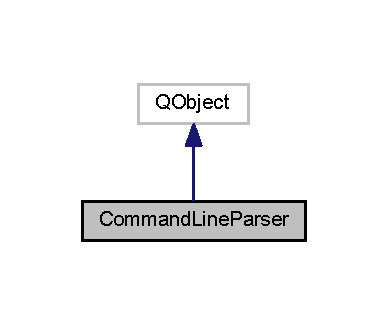
\includegraphics[width=186pt]{class_command_line_parser__inherit__graph}
\end{center}
\end{figure}


Collaboration diagram for Command\-Line\-Parser\-:
\nopagebreak
\begin{figure}[H]
\begin{center}
\leavevmode
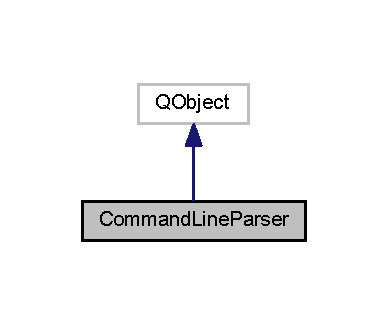
\includegraphics[width=186pt]{class_command_line_parser__coll__graph}
\end{center}
\end{figure}
\subsection*{Public Slots}
\begin{DoxyCompactItemize}
\item 
void \hyperlink{class_command_line_parser_a6a39c14ecf639b02bf8a71ac224b0a61}{Parse\-Arguments} (int argc, char $\ast$$\ast$argv)
\begin{DoxyCompactList}\small\item\em Parses the command-\/line arguments from the ignition function. \end{DoxyCompactList}\end{DoxyCompactItemize}
\subsection*{Public Member Functions}
\begin{DoxyCompactItemize}
\item 
\hyperlink{class_command_line_parser_af9c962bcd44ea242d11b88c9c28bd78d}{Command\-Line\-Parser} (Q\-Object $\ast$parent=0)
\begin{DoxyCompactList}\small\item\em Constructor. \end{DoxyCompactList}\item 
bool \hyperlink{class_command_line_parser_ac50e9de49d6e16174f6d5cf3f89c76d7}{Debugging} ()
\begin{DoxyCompactList}\small\item\em Is the application in debug mode? \end{DoxyCompactList}\item 
bool \hyperlink{class_command_line_parser_aaa2d8544c7841c33c560bb4410144154}{Logging} ()
\begin{DoxyCompactList}\small\item\em Is logging mode enabled? \end{DoxyCompactList}\end{DoxyCompactItemize}


\subsection{Detailed Description}
Deals with arguments passed to the application on the command-\/line. 

The command-\/line parser is created before the main application window is initialised and parses any options sent to the application on the command line. The global instance of the parser is made available through \hyperlink{globals_8h}{globals.\-h} under g\-\_\-p\-Cmd\-Line and several macros exist for facilitating the checking of common global application properties. See \hyperlink{globals_8h}{globals.\-h} for a full description. 

\subsection{Constructor \& Destructor Documentation}
\hypertarget{class_command_line_parser_af9c962bcd44ea242d11b88c9c28bd78d}{\index{Command\-Line\-Parser@{Command\-Line\-Parser}!Command\-Line\-Parser@{Command\-Line\-Parser}}
\index{Command\-Line\-Parser@{Command\-Line\-Parser}!CommandLineParser@{Command\-Line\-Parser}}
\subsubsection[{Command\-Line\-Parser}]{\setlength{\rightskip}{0pt plus 5cm}Command\-Line\-Parser\-::\-Command\-Line\-Parser (
\begin{DoxyParamCaption}
\item[{Q\-Object $\ast$}]{parent = {\ttfamily 0}}
\end{DoxyParamCaption}
)\hspace{0.3cm}{\ttfamily [explicit]}}}\label{class_command_line_parser_af9c962bcd44ea242d11b88c9c28bd78d}


Constructor. 


\begin{DoxyParams}{Parameters}
{\em parent} & Parent object (usually N\-U\-L\-L). \\
\hline
\end{DoxyParams}


\subsection{Member Function Documentation}
\hypertarget{class_command_line_parser_ac50e9de49d6e16174f6d5cf3f89c76d7}{\index{Command\-Line\-Parser@{Command\-Line\-Parser}!Debugging@{Debugging}}
\index{Debugging@{Debugging}!CommandLineParser@{Command\-Line\-Parser}}
\subsubsection[{Debugging}]{\setlength{\rightskip}{0pt plus 5cm}bool Command\-Line\-Parser\-::\-Debugging (
\begin{DoxyParamCaption}
{}
\end{DoxyParamCaption}
)}}\label{class_command_line_parser_ac50e9de49d6e16174f6d5cf3f89c76d7}


Is the application in debug mode? 

\begin{DoxyNote}{Note}
If enabled, the log window is available from the main application Debug menu.

If not specified, debugging mode defaults to false. 
\end{DoxyNote}
\begin{DoxyReturn}{Returns}
True if in debug mode, false otherwise. 
\end{DoxyReturn}
\hypertarget{class_command_line_parser_aaa2d8544c7841c33c560bb4410144154}{\index{Command\-Line\-Parser@{Command\-Line\-Parser}!Logging@{Logging}}
\index{Logging@{Logging}!CommandLineParser@{Command\-Line\-Parser}}
\subsubsection[{Logging}]{\setlength{\rightskip}{0pt plus 5cm}bool Command\-Line\-Parser\-::\-Logging (
\begin{DoxyParamCaption}
{}
\end{DoxyParamCaption}
)}}\label{class_command_line_parser_aaa2d8544c7841c33c560bb4410144154}


Is logging mode enabled? 

\begin{DoxyNote}{Note}
If enabled, logging messsages are written to a log file. If in debug mode, logging mode is also enabled.

If not specified, logging mode defaults to false. 
\end{DoxyNote}
\begin{DoxyReturn}{Returns}
True if enabled, false otherwise. 
\end{DoxyReturn}
\hypertarget{class_command_line_parser_a6a39c14ecf639b02bf8a71ac224b0a61}{\index{Command\-Line\-Parser@{Command\-Line\-Parser}!Parse\-Arguments@{Parse\-Arguments}}
\index{Parse\-Arguments@{Parse\-Arguments}!CommandLineParser@{Command\-Line\-Parser}}
\subsubsection[{Parse\-Arguments}]{\setlength{\rightskip}{0pt plus 5cm}void Command\-Line\-Parser\-::\-Parse\-Arguments (
\begin{DoxyParamCaption}
\item[{int}]{argc, }
\item[{char $\ast$$\ast$}]{argv}
\end{DoxyParamCaption}
)\hspace{0.3cm}{\ttfamily [slot]}}}\label{class_command_line_parser_a6a39c14ecf639b02bf8a71ac224b0a61}


Parses the command-\/line arguments from the ignition function. 


\begin{DoxyParams}{Parameters}
{\em argc} & Number of arguments. \\
\hline
{\em argv} & Char array of arguments. \\
\hline
\end{DoxyParams}


The documentation for this class was generated from the following files\-:\begin{DoxyCompactItemize}
\item 
app/\hyperlink{commandlineparser_8h}{commandlineparser.\-h}\item 
app/commandlineparser.\-cpp\end{DoxyCompactItemize}

\hypertarget{class_command_manager}{\section{Command\-Manager Class Reference}
\label{class_command_manager}\index{Command\-Manager@{Command\-Manager}}
}


Allows quick searching for console commands and variables by their name.  




{\ttfamily \#include $<$commandmanager.\-h$>$}



Inheritance diagram for Command\-Manager\-:\nopagebreak
\begin{figure}[H]
\begin{center}
\leavevmode
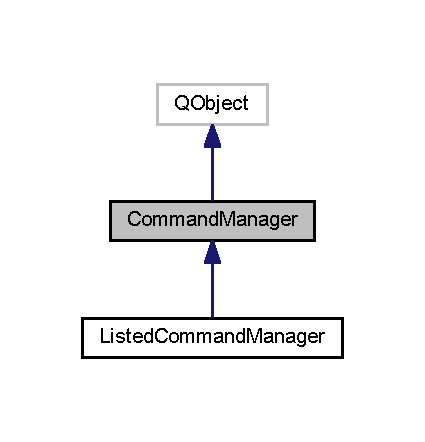
\includegraphics[width=204pt]{class_command_manager__inherit__graph}
\end{center}
\end{figure}


Collaboration diagram for Command\-Manager\-:\nopagebreak
\begin{figure}[H]
\begin{center}
\leavevmode
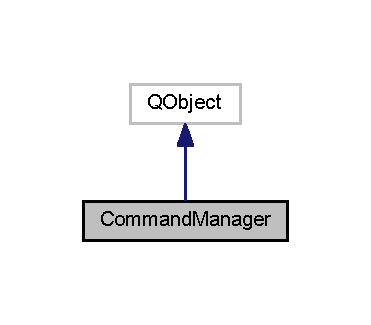
\includegraphics[width=178pt]{class_command_manager__coll__graph}
\end{center}
\end{figure}
\subsection*{Public Types}
\begin{DoxyCompactItemize}
\item 
\hypertarget{class_command_manager_aeaf3c1dd9e4132d9263cc6530d7d988f}{typedef Q\-Map$<$ Q\-String, \\*
\hyperlink{class_base_console_command}{Base\-Console\-Command} $\ast$ $>$ \hyperlink{class_command_manager_aeaf3c1dd9e4132d9263cc6530d7d988f}{Base\-Command\-Map}}\label{class_command_manager_aeaf3c1dd9e4132d9263cc6530d7d988f}

\begin{DoxyCompactList}\small\item\em Typedef for a command entry. The entry contains the name of the command and a \hyperlink{class_base_console_command}{Base\-Console\-Command} pointer to the command object. \end{DoxyCompactList}\end{DoxyCompactItemize}
\subsection*{Signals}
\begin{DoxyCompactItemize}
\item 
\hypertarget{class_command_manager_aabd509f2344154ea7996561c3e9f9807}{void \hyperlink{class_command_manager_aabd509f2344154ea7996561c3e9f9807}{output\-Message} (\hyperlink{class_command_sender_info_a3a5e6a2ef1772f6557f351652c2e3b60}{Command\-Sender\-Info\-::\-Output\-Type}, const Q\-String \&)}\label{class_command_manager_aabd509f2344154ea7996561c3e9f9807}

\begin{DoxyCompactList}\small\item\em Emitted to signal to the command interpreter than output is to be written to the console window. \end{DoxyCompactList}\end{DoxyCompactItemize}
\subsection*{Public Member Functions}
\begin{DoxyCompactItemize}
\item 
\hyperlink{class_command_manager_aec2d1b384154f66d8739cff5fe5430ac}{Command\-Manager} (Q\-Object $\ast$parent=0)
\begin{DoxyCompactList}\small\item\em Constructor. \end{DoxyCompactList}\item 
\hypertarget{class_command_manager_a608ee043482ce1ac1868edb3d21beccf}{virtual \hyperlink{class_command_manager_a608ee043482ce1ac1868edb3d21beccf}{$\sim$\-Command\-Manager} ()}\label{class_command_manager_a608ee043482ce1ac1868edb3d21beccf}

\begin{DoxyCompactList}\small\item\em Destructor. \end{DoxyCompactList}\item 
bool \hyperlink{class_command_manager_a5fbd5a0e340f8aa29e228ad429743f8b}{register\-Command} (\hyperlink{class_base_console_command}{Base\-Console\-Command} $\ast$command)
\begin{DoxyCompactList}\small\item\em Resigters a command into the manager. \end{DoxyCompactList}\item 
void \hyperlink{class_command_manager_ae381ba2ee8706a1def77b356e7a4f7a7}{unregister\-Command} (const Q\-String \&name)
\begin{DoxyCompactList}\small\item\em Unregisters a command by name. \end{DoxyCompactList}\item 
bool \hyperlink{class_command_manager_af105989a8f6a7360295e7d2b7cd61d6e}{is\-Registered} (const Q\-String \&name) const 
\begin{DoxyCompactList}\small\item\em Returns whether the manager holds a command of the given name. \end{DoxyCompactList}\item 
\hyperlink{class_base_console_command}{Base\-Console\-Command} $\ast$ \hyperlink{class_command_manager_ae2c6db5f2f968ac86e34938316cabedc}{get} (const Q\-String \&name) const 
\begin{DoxyCompactList}\small\item\em Retrieves a \hyperlink{class_base_console_command}{Base\-Console\-Command} pointer to the command with the given name. \end{DoxyCompactList}\item 
void \hyperlink{class_command_manager_a51c40a9016fc20bf4aba957982f00164}{find\-Regex} (const Q\-Regular\-Expression \&regex, Q\-List$<$ \hyperlink{class_base_console_command}{Base\-Console\-Command} $\ast$ $>$ \&out\-List, int count=-\/1) const 
\begin{DoxyCompactList}\small\item\em Finds commands whose name matches the given regular expression. \end{DoxyCompactList}\item 
void \hyperlink{class_command_manager_a2b0759f29a6059aed61dd2d2f0b615ab}{find\-Regex} (const Q\-String \&regex, Q\-List$<$ \hyperlink{class_base_console_command}{Base\-Console\-Command} $\ast$ $>$ \&out\-List, int count=-\/1) const 
\begin{DoxyCompactList}\small\item\em Finds commands whose name matches the given regular expression. \end{DoxyCompactList}\item 
void \hyperlink{class_command_manager_ac7c0a660ffb6a1e2e7d0879f58926116}{find\-Prefix} (const Q\-String \&prefix, Q\-List$<$ \hyperlink{class_base_console_command}{Base\-Console\-Command} $\ast$ $>$ \&out\-List, int count=-\/1) const 
\begin{DoxyCompactList}\small\item\em Finds commands whose name matches the given prefix -\/ for returning command suggestions for a partially typed command name. \end{DoxyCompactList}\item 
\hyperlink{class_con_command}{Con\-Command} $\ast$ \hyperlink{class_command_manager_a721e6e49dd5426cff526c567f1912ac8}{get\-Command} (const Q\-String \&name) const 
\begin{DoxyCompactList}\small\item\em Returns a console command with the given name. \end{DoxyCompactList}\item 
\hyperlink{class_con_var}{Con\-Var} $\ast$ \hyperlink{class_command_manager_a1a5e708d4344cec77bc669e72f406075}{get\-Variable} (const Q\-String \&name) const 
\begin{DoxyCompactList}\small\item\em Returns a console variable with the given name. \end{DoxyCompactList}\item 
N\-Global\-Cmd\-::\-Cmd\-Ident \hyperlink{class_command_manager_a80c1150d315f8c15654d86cc2fdbea9d}{exec} (const Q\-String \&name, const Q\-String\-List \&args, int \&ret\-Val, Q\-Variant \&output)
\begin{DoxyCompactList}\small\item\em Executes a command of the given name, with the given arguments, and fills ret\-Val and output with the relevant output data. \end{DoxyCompactList}\item 
Base\-Command\-Map\-::const\-\_\-iterator \hyperlink{class_command_manager_a3c24e4fe95d7e0d030fadda3737d9130}{const\-Begin} ()
\begin{DoxyCompactList}\small\item\em Returns the const\-\_\-iterator representing the beginning of the Q\-Map. \end{DoxyCompactList}\item 
Base\-Command\-Map\-::const\-\_\-iterator \hyperlink{class_command_manager_a96f8aae555bc651fc03c975b334eee82}{const\-End} ()
\begin{DoxyCompactList}\small\item\em Returns the const\-\_\-iterator representing the null item after the end of the Q\-Map. \end{DoxyCompactList}\end{DoxyCompactItemize}


\subsection{Detailed Description}
Allows quick searching for console commands and variables by their name. 

The \hyperlink{class_command_manager}{Command\-Manager} indexes commands in a Q\-Map, providing access to a command in logarithmic time. The commands are alphabetically ordered by name. 

\subsection{Constructor \& Destructor Documentation}
\hypertarget{class_command_manager_aec2d1b384154f66d8739cff5fe5430ac}{\index{Command\-Manager@{Command\-Manager}!Command\-Manager@{Command\-Manager}}
\index{Command\-Manager@{Command\-Manager}!CommandManager@{Command\-Manager}}
\subsubsection[{Command\-Manager}]{\setlength{\rightskip}{0pt plus 5cm}Command\-Manager\-::\-Command\-Manager (
\begin{DoxyParamCaption}
\item[{Q\-Object $\ast$}]{parent = {\ttfamily 0}}
\end{DoxyParamCaption}
)\hspace{0.3cm}{\ttfamily [explicit]}}}\label{class_command_manager_aec2d1b384154f66d8739cff5fe5430ac}


Constructor. 


\begin{DoxyParams}{Parameters}
{\em parent} & Q\-Object parent, if applicable. \\
\hline
\end{DoxyParams}


\subsection{Member Function Documentation}
\hypertarget{class_command_manager_a3c24e4fe95d7e0d030fadda3737d9130}{\index{Command\-Manager@{Command\-Manager}!const\-Begin@{const\-Begin}}
\index{const\-Begin@{const\-Begin}!CommandManager@{Command\-Manager}}
\subsubsection[{const\-Begin}]{\setlength{\rightskip}{0pt plus 5cm}Command\-Manager\-::\-Base\-Command\-Map\-::const\-\_\-iterator Command\-Manager\-::const\-Begin (
\begin{DoxyParamCaption}
{}
\end{DoxyParamCaption}
)}}\label{class_command_manager_a3c24e4fe95d7e0d030fadda3737d9130}


Returns the const\-\_\-iterator representing the beginning of the Q\-Map. 

\begin{DoxyReturn}{Returns}
Const\-\_\-iterator representing the beginning of the Q\-Map. 
\end{DoxyReturn}
\hypertarget{class_command_manager_a96f8aae555bc651fc03c975b334eee82}{\index{Command\-Manager@{Command\-Manager}!const\-End@{const\-End}}
\index{const\-End@{const\-End}!CommandManager@{Command\-Manager}}
\subsubsection[{const\-End}]{\setlength{\rightskip}{0pt plus 5cm}Command\-Manager\-::\-Base\-Command\-Map\-::const\-\_\-iterator Command\-Manager\-::const\-End (
\begin{DoxyParamCaption}
{}
\end{DoxyParamCaption}
)}}\label{class_command_manager_a96f8aae555bc651fc03c975b334eee82}


Returns the const\-\_\-iterator representing the null item after the end of the Q\-Map. 

\begin{DoxyReturn}{Returns}
Const\-\_\-iterator representing the null item after the end of the Q\-Map. 
\end{DoxyReturn}
\hypertarget{class_command_manager_a80c1150d315f8c15654d86cc2fdbea9d}{\index{Command\-Manager@{Command\-Manager}!exec@{exec}}
\index{exec@{exec}!CommandManager@{Command\-Manager}}
\subsubsection[{exec}]{\setlength{\rightskip}{0pt plus 5cm}N\-Global\-Cmd\-::\-Cmd\-Ident Command\-Manager\-::exec (
\begin{DoxyParamCaption}
\item[{const Q\-String \&}]{name, }
\item[{const Q\-String\-List \&}]{args, }
\item[{int \&}]{ret\-Val, }
\item[{Q\-Variant \&}]{output}
\end{DoxyParamCaption}
)}}\label{class_command_manager_a80c1150d315f8c15654d86cc2fdbea9d}


Executes a command of the given name, with the given arguments, and fills ret\-Val and output with the relevant output data. 


\begin{DoxyItemize}
\item If the command is a \hyperlink{class_con_command}{Con\-Command}, {\itshape ret\-Val} holds the return value of the command and the return of this function is N\-Global\-Cmd\-::\-C\-I\-Command. 
\item If the command is a \hyperlink{class_con_var}{Con\-Var}, the first argument in {\itshape args} (if it exists) is taken as the value for the variable to be set to. {\itshape Output} holds the value of the variable (which will be the new value if the variable was set via the arguments). If no argument is specified, the value of and details about the variable are printed to the console window. The return value of the function is N\-Global\-Cmd\-::\-C\-I\-Variable. 
\item If the command is not found, or is neither a \hyperlink{class_con_command}{Con\-Command} nor a \hyperlink{class_con_var}{Con\-Var}, {\itshape ret\-Val} and {\itshape output} are unchanged and the function returns N\-Global\-Cmd\-::\-C\-I\-Null.
\end{DoxyItemize}
\begin{DoxyParams}{Parameters}
{\em name} & Name of command to search for. \\
\hline
{\em args} & Arguments to provide to the command. \\
\hline
{\em ret\-Val} & Holds the return value if the command is a \hyperlink{class_con_command}{Con\-Command}. \\
\hline
{\em output} & Holds the evaluated value of the variable if the command is a \hyperlink{class_con_var}{Con\-Var}. \\
\hline
\end{DoxyParams}
\begin{DoxyReturn}{Returns}
Identifier depending on the type of command that was found. 
\end{DoxyReturn}
\hypertarget{class_command_manager_ac7c0a660ffb6a1e2e7d0879f58926116}{\index{Command\-Manager@{Command\-Manager}!find\-Prefix@{find\-Prefix}}
\index{find\-Prefix@{find\-Prefix}!CommandManager@{Command\-Manager}}
\subsubsection[{find\-Prefix}]{\setlength{\rightskip}{0pt plus 5cm}void Command\-Manager\-::find\-Prefix (
\begin{DoxyParamCaption}
\item[{const Q\-String \&}]{prefix, }
\item[{Q\-List$<$ {\bf Base\-Console\-Command} $\ast$ $>$ \&}]{out\-List, }
\item[{int}]{count = {\ttfamily -\/1}}
\end{DoxyParamCaption}
) const}}\label{class_command_manager_ac7c0a660ffb6a1e2e7d0879f58926116}


Finds commands whose name matches the given prefix -\/ for returning command suggestions for a partially typed command name. 


\begin{DoxyParams}{Parameters}
{\em prefix} & Prefix to search with. \\
\hline
{\em out\-List} & List to fill with pointers to matched commands. \\
\hline
{\em count} & Maximum number of commands to return. -\/1 = no maximum. \\
\hline
\end{DoxyParams}
\hypertarget{class_command_manager_a51c40a9016fc20bf4aba957982f00164}{\index{Command\-Manager@{Command\-Manager}!find\-Regex@{find\-Regex}}
\index{find\-Regex@{find\-Regex}!CommandManager@{Command\-Manager}}
\subsubsection[{find\-Regex}]{\setlength{\rightskip}{0pt plus 5cm}void Command\-Manager\-::find\-Regex (
\begin{DoxyParamCaption}
\item[{const Q\-Regular\-Expression \&}]{regex, }
\item[{Q\-List$<$ {\bf Base\-Console\-Command} $\ast$ $>$ \&}]{out\-List, }
\item[{int}]{count = {\ttfamily -\/1}}
\end{DoxyParamCaption}
) const}}\label{class_command_manager_a51c40a9016fc20bf4aba957982f00164}


Finds commands whose name matches the given regular expression. 


\begin{DoxyParams}{Parameters}
{\em regex} & Regex to match names to. \\
\hline
{\em out\-List} & List to fill with pointers to matched commands. \\
\hline
{\em count} & Maximum number of commands to return. -\/1 = no maximum. \\
\hline
\end{DoxyParams}
\hypertarget{class_command_manager_a2b0759f29a6059aed61dd2d2f0b615ab}{\index{Command\-Manager@{Command\-Manager}!find\-Regex@{find\-Regex}}
\index{find\-Regex@{find\-Regex}!CommandManager@{Command\-Manager}}
\subsubsection[{find\-Regex}]{\setlength{\rightskip}{0pt plus 5cm}void Command\-Manager\-::find\-Regex (
\begin{DoxyParamCaption}
\item[{const Q\-String \&}]{regex, }
\item[{Q\-List$<$ {\bf Base\-Console\-Command} $\ast$ $>$ \&}]{out\-List, }
\item[{int}]{count = {\ttfamily -\/1}}
\end{DoxyParamCaption}
) const}}\label{class_command_manager_a2b0759f29a6059aed61dd2d2f0b615ab}


Finds commands whose name matches the given regular expression. 


\begin{DoxyParams}{Parameters}
{\em regex} & Regex string to match names to. \\
\hline
{\em out\-List} & List to fill with pointers to matched commands. \\
\hline
{\em count} & Maximum number of commands to return. -\/1 = no maximum. \\
\hline
\end{DoxyParams}
\hypertarget{class_command_manager_ae2c6db5f2f968ac86e34938316cabedc}{\index{Command\-Manager@{Command\-Manager}!get@{get}}
\index{get@{get}!CommandManager@{Command\-Manager}}
\subsubsection[{get}]{\setlength{\rightskip}{0pt plus 5cm}{\bf Base\-Console\-Command} $\ast$ Command\-Manager\-::get (
\begin{DoxyParamCaption}
\item[{const Q\-String \&}]{name}
\end{DoxyParamCaption}
) const}}\label{class_command_manager_ae2c6db5f2f968ac86e34938316cabedc}


Retrieves a \hyperlink{class_base_console_command}{Base\-Console\-Command} pointer to the command with the given name. 


\begin{DoxyParams}{Parameters}
{\em name} & Name of command to retrieve. \\
\hline
\end{DoxyParams}
\begin{DoxyReturn}{Returns}
Pointer to command, or N\-U\-L\-L if not found. 
\end{DoxyReturn}
\hypertarget{class_command_manager_a721e6e49dd5426cff526c567f1912ac8}{\index{Command\-Manager@{Command\-Manager}!get\-Command@{get\-Command}}
\index{get\-Command@{get\-Command}!CommandManager@{Command\-Manager}}
\subsubsection[{get\-Command}]{\setlength{\rightskip}{0pt plus 5cm}{\bf Con\-Command} $\ast$ Command\-Manager\-::get\-Command (
\begin{DoxyParamCaption}
\item[{const Q\-String \&}]{name}
\end{DoxyParamCaption}
) const}}\label{class_command_manager_a721e6e49dd5426cff526c567f1912ac8}


Returns a console command with the given name. 


\begin{DoxyParams}{Parameters}
{\em name} & Name of console command to search for. \\
\hline
\end{DoxyParams}
\begin{DoxyReturn}{Returns}
Pointer to command, or N\-U\-L\-L if command didn't exist or did not identify as N\-Global\-Cmd\-::\-C\-I\-Command. 
\end{DoxyReturn}
\hypertarget{class_command_manager_a1a5e708d4344cec77bc669e72f406075}{\index{Command\-Manager@{Command\-Manager}!get\-Variable@{get\-Variable}}
\index{get\-Variable@{get\-Variable}!CommandManager@{Command\-Manager}}
\subsubsection[{get\-Variable}]{\setlength{\rightskip}{0pt plus 5cm}{\bf Con\-Var} $\ast$ Command\-Manager\-::get\-Variable (
\begin{DoxyParamCaption}
\item[{const Q\-String \&}]{name}
\end{DoxyParamCaption}
) const}}\label{class_command_manager_a1a5e708d4344cec77bc669e72f406075}


Returns a console variable with the given name. 


\begin{DoxyParams}{Parameters}
{\em name} & Name of console variable to search for. \\
\hline
\end{DoxyParams}
\begin{DoxyReturn}{Returns}
Pointer to variable, or N\-U\-L\-L if variable didn't exist or did not identify as N\-Global\-Cmd\-::\-C\-I\-Variable. 
\end{DoxyReturn}
\hypertarget{class_command_manager_af105989a8f6a7360295e7d2b7cd61d6e}{\index{Command\-Manager@{Command\-Manager}!is\-Registered@{is\-Registered}}
\index{is\-Registered@{is\-Registered}!CommandManager@{Command\-Manager}}
\subsubsection[{is\-Registered}]{\setlength{\rightskip}{0pt plus 5cm}bool Command\-Manager\-::is\-Registered (
\begin{DoxyParamCaption}
\item[{const Q\-String \&}]{name}
\end{DoxyParamCaption}
) const}}\label{class_command_manager_af105989a8f6a7360295e7d2b7cd61d6e}


Returns whether the manager holds a command of the given name. 


\begin{DoxyParams}{Parameters}
{\em name} & Name of command. \\
\hline
\end{DoxyParams}
\begin{DoxyReturn}{Returns}
True if a command with this name exists in the manager, false otherwise. 
\end{DoxyReturn}
\hypertarget{class_command_manager_a5fbd5a0e340f8aa29e228ad429743f8b}{\index{Command\-Manager@{Command\-Manager}!register\-Command@{register\-Command}}
\index{register\-Command@{register\-Command}!CommandManager@{Command\-Manager}}
\subsubsection[{register\-Command}]{\setlength{\rightskip}{0pt plus 5cm}bool Command\-Manager\-::register\-Command (
\begin{DoxyParamCaption}
\item[{{\bf Base\-Console\-Command} $\ast$}]{command}
\end{DoxyParamCaption}
)}}\label{class_command_manager_a5fbd5a0e340f8aa29e228ad429743f8b}


Resigters a command into the manager. 


\begin{DoxyParams}{Parameters}
{\em command} & Pointer to command to register. \\
\hline
\end{DoxyParams}
\begin{DoxyReturn}{Returns}
True on success, false if a command with the same name was already registered. 
\end{DoxyReturn}
\hypertarget{class_command_manager_ae381ba2ee8706a1def77b356e7a4f7a7}{\index{Command\-Manager@{Command\-Manager}!unregister\-Command@{unregister\-Command}}
\index{unregister\-Command@{unregister\-Command}!CommandManager@{Command\-Manager}}
\subsubsection[{unregister\-Command}]{\setlength{\rightskip}{0pt plus 5cm}void Command\-Manager\-::unregister\-Command (
\begin{DoxyParamCaption}
\item[{const Q\-String \&}]{name}
\end{DoxyParamCaption}
)}}\label{class_command_manager_ae381ba2ee8706a1def77b356e7a4f7a7}


Unregisters a command by name. 


\begin{DoxyParams}{Parameters}
{\em name} & Name of command to remove. \\
\hline
\end{DoxyParams}


The documentation for this class was generated from the following files\-:\begin{DoxyCompactItemize}
\item 
I\-Console/inc/\hyperlink{commandmanager_8h}{commandmanager.\-h}\item 
I\-Console/src/commandmanager.\-cpp\end{DoxyCompactItemize}

\hypertarget{class_command_sender_info}{\section{Command\-Sender\-Info Class Reference}
\label{class_command_sender_info}\index{Command\-Sender\-Info@{Command\-Sender\-Info}}
}


The \hyperlink{class_command_sender_info}{Command\-Sender\-Info} class provides a route between a calling \hyperlink{class_command_manager}{Command\-Manager} and a receiving \hyperlink{class_con_command}{Con\-Command} or \hyperlink{class_con_var}{Con\-Var}. The command or variable can print output to the relevant console window (if one exists) by passing the output to this class.  




{\ttfamily \#include $<$commandsenderinfo.\-h$>$}



Inheritance diagram for Command\-Sender\-Info\-:\nopagebreak
\begin{figure}[H]
\begin{center}
\leavevmode
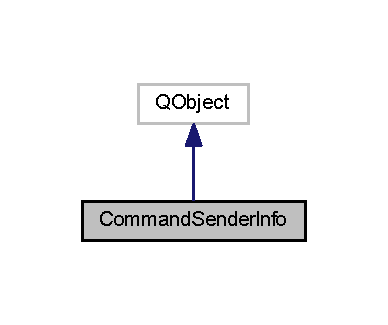
\includegraphics[width=186pt]{class_command_sender_info__inherit__graph}
\end{center}
\end{figure}


Collaboration diagram for Command\-Sender\-Info\-:\nopagebreak
\begin{figure}[H]
\begin{center}
\leavevmode
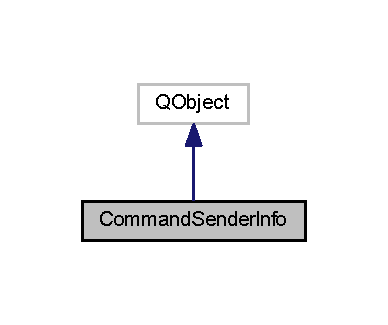
\includegraphics[width=186pt]{class_command_sender_info__coll__graph}
\end{center}
\end{figure}
\subsection*{Public Types}
\begin{DoxyCompactItemize}
\item 
enum \hyperlink{class_command_sender_info_a3a5e6a2ef1772f6557f351652c2e3b60}{Output\-Type} \{ \\*
\hyperlink{class_command_sender_info_a3a5e6a2ef1772f6557f351652c2e3b60a64260c3ff17cea2a0f40e2ed74725f2b}{Output\-General} = 0, 
\hyperlink{class_command_sender_info_a3a5e6a2ef1772f6557f351652c2e3b60a1f1c1e463dbcd5c68f875391a024f520}{Output\-Warning}, 
\hyperlink{class_command_sender_info_a3a5e6a2ef1772f6557f351652c2e3b60a706c899cbfdfa13ffdad7083e52c3fed}{Output\-Custom1}, 
\hyperlink{class_command_sender_info_a3a5e6a2ef1772f6557f351652c2e3b60a2226af7b44b642ccaa3d276171a5e83c}{Output\-Custom2}, 
\\*
\hyperlink{class_command_sender_info_a3a5e6a2ef1772f6557f351652c2e3b60ab3580e2a4b7ce9cd6ceccf36ae3fa852}{Output\-Custom3}, 
\hyperlink{class_command_sender_info_a3a5e6a2ef1772f6557f351652c2e3b60a23562ae85b8c4b677f80813d4a51fdbb}{Output\-Custom4}, 
\hyperlink{class_command_sender_info_a3a5e6a2ef1772f6557f351652c2e3b60a800acfe2330488652d04da3d82474242}{Output\-Custom5}, 
\hyperlink{class_command_sender_info_a3a5e6a2ef1772f6557f351652c2e3b60a60ad31618b524d4c8ce1751cff398133}{Output\-Custom6}
 \}
\begin{DoxyCompactList}\small\item\em Defines the different types of output that can be displayed in a \hyperlink{class_console_widget}{Console\-Widget}. \end{DoxyCompactList}\item 
typedef void(Command\-Manager\-::$\ast$ \hyperlink{class_command_sender_info_a68c494ef69a25ac7bf667b83e24639ed}{Send\-Output} )(\hyperlink{class_command_sender_info_a3a5e6a2ef1772f6557f351652c2e3b60}{Command\-Sender\-Info\-::\-Output\-Type} type, const Q\-String \&msg)
\begin{DoxyCompactList}\small\item\em Typedef for a callback which accepts output from commands. \end{DoxyCompactList}\end{DoxyCompactItemize}
\subsection*{Public Member Functions}
\begin{DoxyCompactItemize}
\item 
\hyperlink{class_command_sender_info_a2e699544abc14568046168b014f4f16e}{Command\-Sender\-Info} (Q\-String name, \hyperlink{class_command_manager}{Command\-Manager} $\ast$manager, \hyperlink{class_command_sender_info_a68c494ef69a25ac7bf667b83e24639ed}{Send\-Output} output\-Func, bool \hyperlink{class_command_sender_info_a9f34e6eb3bab0b16dff37fdacd82695e}{has\-Min}=false, float min=0.\-0f, bool has\-Max=false, float max=0.\-0f, Q\-Object $\ast$parent=0)
\begin{DoxyCompactList}\small\item\em Constructor. \end{DoxyCompactList}\item 
\hyperlink{class_command_sender_info_ae52b21dd10b8c15fa87c6bdbb6f9ed8c}{Command\-Sender\-Info} (const \hyperlink{class_command_sender_info}{Command\-Sender\-Info} \&other)
\begin{DoxyCompactList}\small\item\em Copy constructor. \end{DoxyCompactList}\item 
void \hyperlink{class_command_sender_info_a405f18d255eb60211b373bf58c287d05}{write\-Output} (\hyperlink{class_command_sender_info_a3a5e6a2ef1772f6557f351652c2e3b60}{Command\-Sender\-Info\-::\-Output\-Type} type, const Q\-String \&output) const 
\begin{DoxyCompactList}\small\item\em Sends the output through the output callback stored within this object. \end{DoxyCompactList}\item 
void \hyperlink{class_command_sender_info_a0d081d74145ea6a83502acee2d995e50}{write\-Message} (const Q\-String \&message) const 
\begin{DoxyCompactList}\small\item\em Convenience function -\/ sends a standard message as output. \end{DoxyCompactList}\item 
void \hyperlink{class_command_sender_info_a7c679e9584183f503e322e4149c28dde}{write\-Warning} (const Q\-String \&message) const 
\begin{DoxyCompactList}\small\item\em Convenience function -\/ sends a warning message as output. \end{DoxyCompactList}\item 
\hyperlink{class_command_sender_info_a68c494ef69a25ac7bf667b83e24639ed}{Command\-Sender\-Info\-::\-Send\-Output} \hyperlink{class_command_sender_info_a689dcd3ee607d6f7548f37acfd9545fb}{output\-Callback} () const 
\begin{DoxyCompactList}\small\item\em Returns the pointer to the output callback. \end{DoxyCompactList}\item 
void \hyperlink{class_command_sender_info_a4cd8d7cbb6810d91565534616d3566c3}{set\-Output\-Callback} (\hyperlink{class_command_sender_info_a68c494ef69a25ac7bf667b83e24639ed}{Command\-Sender\-Info\-::\-Send\-Output} output)
\begin{DoxyCompactList}\small\item\em Sets the callback this object will send output through. \end{DoxyCompactList}\item 
Q\-String \hyperlink{class_command_sender_info_ad170306b2bdd8e76016aaf485053f9d7}{command\-Name} () const 
\begin{DoxyCompactList}\small\item\em Gets the name of the command this object was assigned to. \end{DoxyCompactList}\item 
void \hyperlink{class_command_sender_info_a35b041f14c94c82d2fd32d1b2877bc54}{set\-Command\-Name} (Q\-String \&name)
\begin{DoxyCompactList}\small\item\em Sets the name of the command this object is assigned to. \end{DoxyCompactList}\item 
const \hyperlink{class_command_manager}{Command\-Manager} $\ast$ \hyperlink{class_command_sender_info_ab2a5d671d9f8b617a2b15675937b7f53}{command\-Manager} () const 
\begin{DoxyCompactList}\small\item\em Gets the manager this object is assigned to. \end{DoxyCompactList}\item 
void \hyperlink{class_command_sender_info_ab61acf2d7dd2ab6b1eb5376ac611041e}{set\-Command\-Manager} (\hyperlink{class_command_manager}{Command\-Manager} $\ast$manager)
\begin{DoxyCompactList}\small\item\em Sets the manager this object is assigned to. \end{DoxyCompactList}\item 
bool \hyperlink{class_command_sender_info_a0535d20518b5f3dbb358d027784e63fe}{has\-Min} () const 
\begin{DoxyCompactList}\small\item\em Returns whether the variable has a min value. \end{DoxyCompactList}\item 
void \hyperlink{class_command_sender_info_ac46d887956a3edbadc8375a97c85b38f}{set\-Has\-Min} (bool b)
\begin{DoxyCompactList}\small\item\em Sets whether the variable has a min value. \end{DoxyCompactList}\item 
bool \hyperlink{class_command_sender_info_afc6b456de58752c0601f635927c72852}{has\-Max} () const 
\begin{DoxyCompactList}\small\item\em Returns whether the variable has a max value. \end{DoxyCompactList}\item 
void \hyperlink{class_command_sender_info_a69ac1e0453b2a79bc697def44a8d356e}{set\-Has\-Max} (bool b)
\begin{DoxyCompactList}\small\item\em Sets whether the variable has a max value. \end{DoxyCompactList}\item 
float \hyperlink{class_command_sender_info_aa3d7b4f7a78bcc0c0f882b6a479b74dc}{min\-Value} () const 
\begin{DoxyCompactList}\small\item\em Gets the variable's min value. \end{DoxyCompactList}\item 
void \hyperlink{class_command_sender_info_ad1e49e6c18b5d75aacb8c7c68a79ed76}{set\-Min\-Value} (float val)
\begin{DoxyCompactList}\small\item\em Sets the variable's min value. \end{DoxyCompactList}\item 
float \hyperlink{class_command_sender_info_a187eae30c2bc2a2ab98d2cf09bad4a13}{max\-Value} () const 
\begin{DoxyCompactList}\small\item\em Gets the variable's max value. \end{DoxyCompactList}\item 
void \hyperlink{class_command_sender_info_af57f1c16ede28190022994e75206223f}{set\-Max\-Value} (float val)
\begin{DoxyCompactList}\small\item\em Sets the variable's max value. \end{DoxyCompactList}\end{DoxyCompactItemize}
\subsection*{Properties}
\begin{DoxyCompactItemize}
\item 
\hyperlink{class_command_sender_info_a68c494ef69a25ac7bf667b83e24639ed}{Send\-Output} \hyperlink{class_command_sender_info_af04b4cc7b75a48a4583411c1c130d654}{output\-Callback}
\begin{DoxyCompactList}\small\item\em Callback to send output through. \end{DoxyCompactList}\item 
Q\-String \hyperlink{class_command_sender_info_af9825e2019cac0c5c9793eefe8086b6c}{command\-Name}
\begin{DoxyCompactList}\small\item\em Name of command this object is assigned to. \end{DoxyCompactList}\item 
bool \hyperlink{class_command_sender_info_a9f34e6eb3bab0b16dff37fdacd82695e}{has\-Min}
\begin{DoxyCompactList}\small\item\em Whether the variable has a min value. Only used for Con\-Vars. \end{DoxyCompactList}\item 
bool \hyperlink{class_command_sender_info_ae003e4ee143379be99e52bbe6dce3a69}{has\-Max}
\begin{DoxyCompactList}\small\item\em Whether the variable has a max value. Only used for Con\-Vars. \end{DoxyCompactList}\item 
float \hyperlink{class_command_sender_info_a7279460303b092c8d78735bd33e94ae0}{min\-Value}
\begin{DoxyCompactList}\small\item\em Variable's min value. Only used for Con\-Vars. \end{DoxyCompactList}\item 
float \hyperlink{class_command_sender_info_ac5b816de5b4e61339e0b649bd8f58799}{max\-Value}
\begin{DoxyCompactList}\small\item\em Variable's max value. Only used for Con\-Vars. \end{DoxyCompactList}\end{DoxyCompactItemize}
\subsection*{Friends}
\begin{DoxyCompactItemize}
\item 
\hypertarget{class_command_sender_info_a5ee157709621d8775061d944a62ed7fa}{class {\bfseries Command\-Sender\-Info}}\label{class_command_sender_info_a5ee157709621d8775061d944a62ed7fa}

\end{DoxyCompactItemize}


\subsection{Detailed Description}
The \hyperlink{class_command_sender_info}{Command\-Sender\-Info} class provides a route between a calling \hyperlink{class_command_manager}{Command\-Manager} and a receiving \hyperlink{class_con_command}{Con\-Command} or \hyperlink{class_con_var}{Con\-Var}. The command or variable can print output to the relevant console window (if one exists) by passing the output to this class. 

\subsection{Member Typedef Documentation}
\hypertarget{class_command_sender_info_a68c494ef69a25ac7bf667b83e24639ed}{\index{Command\-Sender\-Info@{Command\-Sender\-Info}!Send\-Output@{Send\-Output}}
\index{Send\-Output@{Send\-Output}!CommandSenderInfo@{Command\-Sender\-Info}}
\subsubsection[{Send\-Output}]{\setlength{\rightskip}{0pt plus 5cm}typedef void(Command\-Manager\-::$\ast$ Command\-Sender\-Info\-::\-Send\-Output)({\bf Command\-Sender\-Info\-::\-Output\-Type} type, const Q\-String \&msg)}}\label{class_command_sender_info_a68c494ef69a25ac7bf667b83e24639ed}


Typedef for a callback which accepts output from commands. 


\begin{DoxyParams}{Parameters}
{\em type} & Type of output to display. \\
\hline
{\em msg} & Output message. \\
\hline
\end{DoxyParams}


\subsection{Member Enumeration Documentation}
\hypertarget{class_command_sender_info_a3a5e6a2ef1772f6557f351652c2e3b60}{\index{Command\-Sender\-Info@{Command\-Sender\-Info}!Output\-Type@{Output\-Type}}
\index{Output\-Type@{Output\-Type}!CommandSenderInfo@{Command\-Sender\-Info}}
\subsubsection[{Output\-Type}]{\setlength{\rightskip}{0pt plus 5cm}enum {\bf Command\-Sender\-Info\-::\-Output\-Type}}}\label{class_command_sender_info_a3a5e6a2ef1772f6557f351652c2e3b60}


Defines the different types of output that can be displayed in a \hyperlink{class_console_widget}{Console\-Widget}. 

\begin{Desc}
\item[Enumerator]\par
\begin{description}
\index{Output\-General@{Output\-General}!Command\-Sender\-Info@{Command\-Sender\-Info}}\index{Command\-Sender\-Info@{Command\-Sender\-Info}!Output\-General@{Output\-General}}\item[{\em 
\hypertarget{class_command_sender_info_a3a5e6a2ef1772f6557f351652c2e3b60a64260c3ff17cea2a0f40e2ed74725f2b}{Output\-General}\label{class_command_sender_info_a3a5e6a2ef1772f6557f351652c2e3b60a64260c3ff17cea2a0f40e2ed74725f2b}
}]Standard message \index{Output\-Warning@{Output\-Warning}!Command\-Sender\-Info@{Command\-Sender\-Info}}\index{Command\-Sender\-Info@{Command\-Sender\-Info}!Output\-Warning@{Output\-Warning}}\item[{\em 
\hypertarget{class_command_sender_info_a3a5e6a2ef1772f6557f351652c2e3b60a1f1c1e463dbcd5c68f875391a024f520}{Output\-Warning}\label{class_command_sender_info_a3a5e6a2ef1772f6557f351652c2e3b60a1f1c1e463dbcd5c68f875391a024f520}
}]Warning \index{Output\-Custom1@{Output\-Custom1}!Command\-Sender\-Info@{Command\-Sender\-Info}}\index{Command\-Sender\-Info@{Command\-Sender\-Info}!Output\-Custom1@{Output\-Custom1}}\item[{\em 
\hypertarget{class_command_sender_info_a3a5e6a2ef1772f6557f351652c2e3b60a706c899cbfdfa13ffdad7083e52c3fed}{Output\-Custom1}\label{class_command_sender_info_a3a5e6a2ef1772f6557f351652c2e3b60a706c899cbfdfa13ffdad7083e52c3fed}
}]Custom type 1 -\/ usually inactive text \index{Output\-Custom2@{Output\-Custom2}!Command\-Sender\-Info@{Command\-Sender\-Info}}\index{Command\-Sender\-Info@{Command\-Sender\-Info}!Output\-Custom2@{Output\-Custom2}}\item[{\em 
\hypertarget{class_command_sender_info_a3a5e6a2ef1772f6557f351652c2e3b60a2226af7b44b642ccaa3d276171a5e83c}{Output\-Custom2}\label{class_command_sender_info_a3a5e6a2ef1772f6557f351652c2e3b60a2226af7b44b642ccaa3d276171a5e83c}
}]Custom type 2 -\/ usually highlighted or otherwise important text \index{Output\-Custom3@{Output\-Custom3}!Command\-Sender\-Info@{Command\-Sender\-Info}}\index{Command\-Sender\-Info@{Command\-Sender\-Info}!Output\-Custom3@{Output\-Custom3}}\item[{\em 
\hypertarget{class_command_sender_info_a3a5e6a2ef1772f6557f351652c2e3b60ab3580e2a4b7ce9cd6ceccf36ae3fa852}{Output\-Custom3}\label{class_command_sender_info_a3a5e6a2ef1772f6557f351652c2e3b60ab3580e2a4b7ce9cd6ceccf36ae3fa852}
}]Custom type 3 \index{Output\-Custom4@{Output\-Custom4}!Command\-Sender\-Info@{Command\-Sender\-Info}}\index{Command\-Sender\-Info@{Command\-Sender\-Info}!Output\-Custom4@{Output\-Custom4}}\item[{\em 
\hypertarget{class_command_sender_info_a3a5e6a2ef1772f6557f351652c2e3b60a23562ae85b8c4b677f80813d4a51fdbb}{Output\-Custom4}\label{class_command_sender_info_a3a5e6a2ef1772f6557f351652c2e3b60a23562ae85b8c4b677f80813d4a51fdbb}
}]Custom type 4 \index{Output\-Custom5@{Output\-Custom5}!Command\-Sender\-Info@{Command\-Sender\-Info}}\index{Command\-Sender\-Info@{Command\-Sender\-Info}!Output\-Custom5@{Output\-Custom5}}\item[{\em 
\hypertarget{class_command_sender_info_a3a5e6a2ef1772f6557f351652c2e3b60a800acfe2330488652d04da3d82474242}{Output\-Custom5}\label{class_command_sender_info_a3a5e6a2ef1772f6557f351652c2e3b60a800acfe2330488652d04da3d82474242}
}]Custom type 5 \index{Output\-Custom6@{Output\-Custom6}!Command\-Sender\-Info@{Command\-Sender\-Info}}\index{Command\-Sender\-Info@{Command\-Sender\-Info}!Output\-Custom6@{Output\-Custom6}}\item[{\em 
\hypertarget{class_command_sender_info_a3a5e6a2ef1772f6557f351652c2e3b60a60ad31618b524d4c8ce1751cff398133}{Output\-Custom6}\label{class_command_sender_info_a3a5e6a2ef1772f6557f351652c2e3b60a60ad31618b524d4c8ce1751cff398133}
}]Custom type 6 \end{description}
\end{Desc}


\subsection{Constructor \& Destructor Documentation}
\hypertarget{class_command_sender_info_a2e699544abc14568046168b014f4f16e}{\index{Command\-Sender\-Info@{Command\-Sender\-Info}!Command\-Sender\-Info@{Command\-Sender\-Info}}
\index{Command\-Sender\-Info@{Command\-Sender\-Info}!CommandSenderInfo@{Command\-Sender\-Info}}
\subsubsection[{Command\-Sender\-Info}]{\setlength{\rightskip}{0pt plus 5cm}Command\-Sender\-Info\-::\-Command\-Sender\-Info (
\begin{DoxyParamCaption}
\item[{Q\-String}]{name, }
\item[{{\bf Command\-Manager} $\ast$}]{manager, }
\item[{{\bf Send\-Output}}]{output\-Func, }
\item[{bool}]{has\-Min = {\ttfamily false}, }
\item[{float}]{min = {\ttfamily 0.0f}, }
\item[{bool}]{has\-Max = {\ttfamily false}, }
\item[{float}]{max = {\ttfamily 0.0f}, }
\item[{Q\-Object $\ast$}]{parent = {\ttfamily 0}}
\end{DoxyParamCaption}
)\hspace{0.3cm}{\ttfamily [explicit]}}}\label{class_command_sender_info_a2e699544abc14568046168b014f4f16e}


Constructor. 


\begin{DoxyParams}{Parameters}
{\em name} & Name of command or variable we are passing data to. Informational only. \\
\hline
{\em manager} & Command's manager. \\
\hline
{\em output\-Func} & Pointer to function which the command can write output through. \\
\hline
{\em has\-Min} & Whether the variable has a minimum value. Informational only. \\
\hline
{\em min} & Minimum value of the variable. Informational only. \\
\hline
{\em has\-Max} & Whether the variable has a maximum value. Informational only. \\
\hline
{\em max} & Maximum value of the variable. Informational only. \\
\hline
{\em parent} & Q\-Object parent, if applicable. \\
\hline
\end{DoxyParams}
\hypertarget{class_command_sender_info_ae52b21dd10b8c15fa87c6bdbb6f9ed8c}{\index{Command\-Sender\-Info@{Command\-Sender\-Info}!Command\-Sender\-Info@{Command\-Sender\-Info}}
\index{Command\-Sender\-Info@{Command\-Sender\-Info}!CommandSenderInfo@{Command\-Sender\-Info}}
\subsubsection[{Command\-Sender\-Info}]{\setlength{\rightskip}{0pt plus 5cm}Command\-Sender\-Info\-::\-Command\-Sender\-Info (
\begin{DoxyParamCaption}
\item[{const {\bf Command\-Sender\-Info} \&}]{other}
\end{DoxyParamCaption}
)}}\label{class_command_sender_info_ae52b21dd10b8c15fa87c6bdbb6f9ed8c}


Copy constructor. 

\begin{DoxyNote}{Note}
As per Qt's architecture, similar Q\-Objects are not {\itshape copies} of each other, just different instances of the same object. 
\end{DoxyNote}

\begin{DoxyParams}{Parameters}
{\em other} & \hyperlink{class_command_sender_info}{Command\-Sender\-Info} to copy values from. \\
\hline
\end{DoxyParams}


\subsection{Member Function Documentation}
\hypertarget{class_command_sender_info_ab2a5d671d9f8b617a2b15675937b7f53}{\index{Command\-Sender\-Info@{Command\-Sender\-Info}!command\-Manager@{command\-Manager}}
\index{command\-Manager@{command\-Manager}!CommandSenderInfo@{Command\-Sender\-Info}}
\subsubsection[{command\-Manager}]{\setlength{\rightskip}{0pt plus 5cm}const {\bf Command\-Manager} $\ast$ Command\-Sender\-Info\-::command\-Manager (
\begin{DoxyParamCaption}
{}
\end{DoxyParamCaption}
) const}}\label{class_command_sender_info_ab2a5d671d9f8b617a2b15675937b7f53}


Gets the manager this object is assigned to. 

\begin{DoxyReturn}{Returns}
Pointer to manager. 
\end{DoxyReturn}
\hypertarget{class_command_sender_info_ad170306b2bdd8e76016aaf485053f9d7}{\index{Command\-Sender\-Info@{Command\-Sender\-Info}!command\-Name@{command\-Name}}
\index{command\-Name@{command\-Name}!CommandSenderInfo@{Command\-Sender\-Info}}
\subsubsection[{command\-Name}]{\setlength{\rightskip}{0pt plus 5cm}Q\-String Command\-Sender\-Info\-::command\-Name (
\begin{DoxyParamCaption}
{}
\end{DoxyParamCaption}
) const}}\label{class_command_sender_info_ad170306b2bdd8e76016aaf485053f9d7}


Gets the name of the command this object was assigned to. 

\begin{DoxyReturn}{Returns}
Name of object. 
\end{DoxyReturn}
\hypertarget{class_command_sender_info_afc6b456de58752c0601f635927c72852}{\index{Command\-Sender\-Info@{Command\-Sender\-Info}!has\-Max@{has\-Max}}
\index{has\-Max@{has\-Max}!CommandSenderInfo@{Command\-Sender\-Info}}
\subsubsection[{has\-Max}]{\setlength{\rightskip}{0pt plus 5cm}bool Command\-Sender\-Info\-::has\-Max (
\begin{DoxyParamCaption}
{}
\end{DoxyParamCaption}
) const}}\label{class_command_sender_info_afc6b456de58752c0601f635927c72852}


Returns whether the variable has a max value. 

\begin{DoxyNote}{Note}
Only relevant for \hyperlink{class_con_var}{Con\-Var} callbacks. Informational only. 
\end{DoxyNote}
\begin{DoxyReturn}{Returns}
True if the variable has a max value, false otherwise. 
\end{DoxyReturn}
\hypertarget{class_command_sender_info_a0535d20518b5f3dbb358d027784e63fe}{\index{Command\-Sender\-Info@{Command\-Sender\-Info}!has\-Min@{has\-Min}}
\index{has\-Min@{has\-Min}!CommandSenderInfo@{Command\-Sender\-Info}}
\subsubsection[{has\-Min}]{\setlength{\rightskip}{0pt plus 5cm}bool Command\-Sender\-Info\-::has\-Min (
\begin{DoxyParamCaption}
{}
\end{DoxyParamCaption}
) const}}\label{class_command_sender_info_a0535d20518b5f3dbb358d027784e63fe}


Returns whether the variable has a min value. 

\begin{DoxyNote}{Note}
Only relevant for \hyperlink{class_con_var}{Con\-Var} callbacks. Informational only. 
\end{DoxyNote}
\begin{DoxyReturn}{Returns}
True if the variable has a min value, false otherwise. 
\end{DoxyReturn}
\hypertarget{class_command_sender_info_a187eae30c2bc2a2ab98d2cf09bad4a13}{\index{Command\-Sender\-Info@{Command\-Sender\-Info}!max\-Value@{max\-Value}}
\index{max\-Value@{max\-Value}!CommandSenderInfo@{Command\-Sender\-Info}}
\subsubsection[{max\-Value}]{\setlength{\rightskip}{0pt plus 5cm}float Command\-Sender\-Info\-::max\-Value (
\begin{DoxyParamCaption}
{}
\end{DoxyParamCaption}
) const}}\label{class_command_sender_info_a187eae30c2bc2a2ab98d2cf09bad4a13}


Gets the variable's max value. 

\begin{DoxyNote}{Note}
Only relevant for \hyperlink{class_con_var}{Con\-Var} callbacks. Informational only. 
\end{DoxyNote}
\begin{DoxyWarning}{Warning}
If the variable does not have a maximum value, the return of this function is undefined. 
\end{DoxyWarning}
\begin{DoxyReturn}{Returns}
Maximum value of the variable. 
\end{DoxyReturn}
\hypertarget{class_command_sender_info_aa3d7b4f7a78bcc0c0f882b6a479b74dc}{\index{Command\-Sender\-Info@{Command\-Sender\-Info}!min\-Value@{min\-Value}}
\index{min\-Value@{min\-Value}!CommandSenderInfo@{Command\-Sender\-Info}}
\subsubsection[{min\-Value}]{\setlength{\rightskip}{0pt plus 5cm}float Command\-Sender\-Info\-::min\-Value (
\begin{DoxyParamCaption}
{}
\end{DoxyParamCaption}
) const}}\label{class_command_sender_info_aa3d7b4f7a78bcc0c0f882b6a479b74dc}


Gets the variable's min value. 

\begin{DoxyNote}{Note}
Only relevant for \hyperlink{class_con_var}{Con\-Var} callbacks. Informational only. 
\end{DoxyNote}
\begin{DoxyWarning}{Warning}
If the variable does not have a minimum value, the return of this function is undefined. 
\end{DoxyWarning}
\begin{DoxyReturn}{Returns}
Minimum value of the variable. 
\end{DoxyReturn}
\hypertarget{class_command_sender_info_a689dcd3ee607d6f7548f37acfd9545fb}{\index{Command\-Sender\-Info@{Command\-Sender\-Info}!output\-Callback@{output\-Callback}}
\index{output\-Callback@{output\-Callback}!CommandSenderInfo@{Command\-Sender\-Info}}
\subsubsection[{output\-Callback}]{\setlength{\rightskip}{0pt plus 5cm}{\bf Command\-Sender\-Info\-::\-Send\-Output} Command\-Sender\-Info\-::output\-Callback (
\begin{DoxyParamCaption}
{}
\end{DoxyParamCaption}
) const}}\label{class_command_sender_info_a689dcd3ee607d6f7548f37acfd9545fb}


Returns the pointer to the output callback. 

\begin{DoxyReturn}{Returns}
Callback pointer. 
\end{DoxyReturn}
\hypertarget{class_command_sender_info_ab61acf2d7dd2ab6b1eb5376ac611041e}{\index{Command\-Sender\-Info@{Command\-Sender\-Info}!set\-Command\-Manager@{set\-Command\-Manager}}
\index{set\-Command\-Manager@{set\-Command\-Manager}!CommandSenderInfo@{Command\-Sender\-Info}}
\subsubsection[{set\-Command\-Manager}]{\setlength{\rightskip}{0pt plus 5cm}void Command\-Sender\-Info\-::set\-Command\-Manager (
\begin{DoxyParamCaption}
\item[{{\bf Command\-Manager} $\ast$}]{manager}
\end{DoxyParamCaption}
)}}\label{class_command_sender_info_ab61acf2d7dd2ab6b1eb5376ac611041e}


Sets the manager this object is assigned to. 


\begin{DoxyParams}{Parameters}
{\em manager} & Manager to set. \\
\hline
\end{DoxyParams}
\hypertarget{class_command_sender_info_a35b041f14c94c82d2fd32d1b2877bc54}{\index{Command\-Sender\-Info@{Command\-Sender\-Info}!set\-Command\-Name@{set\-Command\-Name}}
\index{set\-Command\-Name@{set\-Command\-Name}!CommandSenderInfo@{Command\-Sender\-Info}}
\subsubsection[{set\-Command\-Name}]{\setlength{\rightskip}{0pt plus 5cm}void Command\-Sender\-Info\-::set\-Command\-Name (
\begin{DoxyParamCaption}
\item[{Q\-String \&}]{name}
\end{DoxyParamCaption}
)}}\label{class_command_sender_info_a35b041f14c94c82d2fd32d1b2877bc54}


Sets the name of the command this object is assigned to. 


\begin{DoxyParams}{Parameters}
{\em name} & Name to set. \\
\hline
\end{DoxyParams}
\hypertarget{class_command_sender_info_a69ac1e0453b2a79bc697def44a8d356e}{\index{Command\-Sender\-Info@{Command\-Sender\-Info}!set\-Has\-Max@{set\-Has\-Max}}
\index{set\-Has\-Max@{set\-Has\-Max}!CommandSenderInfo@{Command\-Sender\-Info}}
\subsubsection[{set\-Has\-Max}]{\setlength{\rightskip}{0pt plus 5cm}void Command\-Sender\-Info\-::set\-Has\-Max (
\begin{DoxyParamCaption}
\item[{bool}]{b}
\end{DoxyParamCaption}
)}}\label{class_command_sender_info_a69ac1e0453b2a79bc697def44a8d356e}


Sets whether the variable has a max value. 

\begin{DoxyNote}{Note}
Only relevant for \hyperlink{class_con_var}{Con\-Var} callbacks. This is informational only and has no effect on the actual variable. 
\end{DoxyNote}

\begin{DoxyParams}{Parameters}
{\em b} & True if the variable should have a max value, false otherwise. \\
\hline
\end{DoxyParams}
\hypertarget{class_command_sender_info_ac46d887956a3edbadc8375a97c85b38f}{\index{Command\-Sender\-Info@{Command\-Sender\-Info}!set\-Has\-Min@{set\-Has\-Min}}
\index{set\-Has\-Min@{set\-Has\-Min}!CommandSenderInfo@{Command\-Sender\-Info}}
\subsubsection[{set\-Has\-Min}]{\setlength{\rightskip}{0pt plus 5cm}void Command\-Sender\-Info\-::set\-Has\-Min (
\begin{DoxyParamCaption}
\item[{bool}]{b}
\end{DoxyParamCaption}
)}}\label{class_command_sender_info_ac46d887956a3edbadc8375a97c85b38f}


Sets whether the variable has a min value. 

\begin{DoxyNote}{Note}
Only relevant for \hyperlink{class_con_var}{Con\-Var} callbacks. This is informational only and has no effect on the actual variable. 
\end{DoxyNote}

\begin{DoxyParams}{Parameters}
{\em b} & True if the variable should have a min value, false otherwise. \\
\hline
\end{DoxyParams}
\hypertarget{class_command_sender_info_af57f1c16ede28190022994e75206223f}{\index{Command\-Sender\-Info@{Command\-Sender\-Info}!set\-Max\-Value@{set\-Max\-Value}}
\index{set\-Max\-Value@{set\-Max\-Value}!CommandSenderInfo@{Command\-Sender\-Info}}
\subsubsection[{set\-Max\-Value}]{\setlength{\rightskip}{0pt plus 5cm}void Command\-Sender\-Info\-::set\-Max\-Value (
\begin{DoxyParamCaption}
\item[{float}]{val}
\end{DoxyParamCaption}
)}}\label{class_command_sender_info_af57f1c16ede28190022994e75206223f}


Sets the variable's max value. 

\begin{DoxyNote}{Note}
Only relevant for \hyperlink{class_con_var}{Con\-Var} callbacks.\-This is informational only and has no effect on the actual variable. 
\end{DoxyNote}

\begin{DoxyParams}{Parameters}
{\em val} & Value of the max bound. \\
\hline
\end{DoxyParams}
\hypertarget{class_command_sender_info_ad1e49e6c18b5d75aacb8c7c68a79ed76}{\index{Command\-Sender\-Info@{Command\-Sender\-Info}!set\-Min\-Value@{set\-Min\-Value}}
\index{set\-Min\-Value@{set\-Min\-Value}!CommandSenderInfo@{Command\-Sender\-Info}}
\subsubsection[{set\-Min\-Value}]{\setlength{\rightskip}{0pt plus 5cm}void Command\-Sender\-Info\-::set\-Min\-Value (
\begin{DoxyParamCaption}
\item[{float}]{val}
\end{DoxyParamCaption}
)}}\label{class_command_sender_info_ad1e49e6c18b5d75aacb8c7c68a79ed76}


Sets the variable's min value. 

\begin{DoxyNote}{Note}
Only relevant for \hyperlink{class_con_var}{Con\-Var} callbacks. This is informational only and has no effect on the actual variable. 
\end{DoxyNote}

\begin{DoxyParams}{Parameters}
{\em val} & Value of the min bound. \\
\hline
\end{DoxyParams}
\hypertarget{class_command_sender_info_a4cd8d7cbb6810d91565534616d3566c3}{\index{Command\-Sender\-Info@{Command\-Sender\-Info}!set\-Output\-Callback@{set\-Output\-Callback}}
\index{set\-Output\-Callback@{set\-Output\-Callback}!CommandSenderInfo@{Command\-Sender\-Info}}
\subsubsection[{set\-Output\-Callback}]{\setlength{\rightskip}{0pt plus 5cm}void Command\-Sender\-Info\-::set\-Output\-Callback (
\begin{DoxyParamCaption}
\item[{{\bf Command\-Sender\-Info\-::\-Send\-Output}}]{output}
\end{DoxyParamCaption}
)}}\label{class_command_sender_info_a4cd8d7cbb6810d91565534616d3566c3}


Sets the callback this object will send output through. 


\begin{DoxyParams}{Parameters}
{\em output} & Pointer to set. \\
\hline
\end{DoxyParams}
\hypertarget{class_command_sender_info_a0d081d74145ea6a83502acee2d995e50}{\index{Command\-Sender\-Info@{Command\-Sender\-Info}!write\-Message@{write\-Message}}
\index{write\-Message@{write\-Message}!CommandSenderInfo@{Command\-Sender\-Info}}
\subsubsection[{write\-Message}]{\setlength{\rightskip}{0pt plus 5cm}void Command\-Sender\-Info\-::write\-Message (
\begin{DoxyParamCaption}
\item[{const Q\-String \&}]{message}
\end{DoxyParamCaption}
) const}}\label{class_command_sender_info_a0d081d74145ea6a83502acee2d995e50}


Convenience function -\/ sends a standard message as output. 


\begin{DoxyParams}{Parameters}
{\em message} & Output message. \\
\hline
\end{DoxyParams}
\hypertarget{class_command_sender_info_a405f18d255eb60211b373bf58c287d05}{\index{Command\-Sender\-Info@{Command\-Sender\-Info}!write\-Output@{write\-Output}}
\index{write\-Output@{write\-Output}!CommandSenderInfo@{Command\-Sender\-Info}}
\subsubsection[{write\-Output}]{\setlength{\rightskip}{0pt plus 5cm}void Command\-Sender\-Info\-::write\-Output (
\begin{DoxyParamCaption}
\item[{{\bf Command\-Sender\-Info\-::\-Output\-Type}}]{type, }
\item[{const Q\-String \&}]{output}
\end{DoxyParamCaption}
) const}}\label{class_command_sender_info_a405f18d255eb60211b373bf58c287d05}


Sends the output through the output callback stored within this object. 


\begin{DoxyParams}{Parameters}
{\em type} & Type of output to display. \\
\hline
{\em output} & Output message. \\
\hline
\end{DoxyParams}
\hypertarget{class_command_sender_info_a7c679e9584183f503e322e4149c28dde}{\index{Command\-Sender\-Info@{Command\-Sender\-Info}!write\-Warning@{write\-Warning}}
\index{write\-Warning@{write\-Warning}!CommandSenderInfo@{Command\-Sender\-Info}}
\subsubsection[{write\-Warning}]{\setlength{\rightskip}{0pt plus 5cm}void Command\-Sender\-Info\-::write\-Warning (
\begin{DoxyParamCaption}
\item[{const Q\-String \&}]{message}
\end{DoxyParamCaption}
) const}}\label{class_command_sender_info_a7c679e9584183f503e322e4149c28dde}


Convenience function -\/ sends a warning message as output. 


\begin{DoxyParams}{Parameters}
{\em message} & Warning message. \\
\hline
\end{DoxyParams}


\subsection{Property Documentation}
\hypertarget{class_command_sender_info_af9825e2019cac0c5c9793eefe8086b6c}{\index{Command\-Sender\-Info@{Command\-Sender\-Info}!command\-Name@{command\-Name}}
\index{command\-Name@{command\-Name}!CommandSenderInfo@{Command\-Sender\-Info}}
\subsubsection[{command\-Name}]{\setlength{\rightskip}{0pt plus 5cm}Q\-String Command\-Sender\-Info\-::command\-Name\hspace{0.3cm}{\ttfamily [read]}, {\ttfamily [write]}}}\label{class_command_sender_info_af9825e2019cac0c5c9793eefe8086b6c}


Name of command this object is assigned to. 

\begin{DoxyParagraph}{Accessors\-:}
\hyperlink{class_command_sender_info_af9825e2019cac0c5c9793eefe8086b6c}{command\-Name()}, \hyperlink{class_command_sender_info_a35b041f14c94c82d2fd32d1b2877bc54}{set\-Command\-Name()} 
\end{DoxyParagraph}
\hypertarget{class_command_sender_info_ae003e4ee143379be99e52bbe6dce3a69}{\index{Command\-Sender\-Info@{Command\-Sender\-Info}!has\-Max@{has\-Max}}
\index{has\-Max@{has\-Max}!CommandSenderInfo@{Command\-Sender\-Info}}
\subsubsection[{has\-Max}]{\setlength{\rightskip}{0pt plus 5cm}bool Command\-Sender\-Info\-::has\-Max\hspace{0.3cm}{\ttfamily [read]}, {\ttfamily [write]}}}\label{class_command_sender_info_ae003e4ee143379be99e52bbe6dce3a69}


Whether the variable has a max value. Only used for Con\-Vars. 

\begin{DoxyParagraph}{Accessors\-:}
\hyperlink{class_command_sender_info_ae003e4ee143379be99e52bbe6dce3a69}{has\-Max()}, \hyperlink{class_command_sender_info_a69ac1e0453b2a79bc697def44a8d356e}{set\-Has\-Max()} 
\end{DoxyParagraph}
\hypertarget{class_command_sender_info_a9f34e6eb3bab0b16dff37fdacd82695e}{\index{Command\-Sender\-Info@{Command\-Sender\-Info}!has\-Min@{has\-Min}}
\index{has\-Min@{has\-Min}!CommandSenderInfo@{Command\-Sender\-Info}}
\subsubsection[{has\-Min}]{\setlength{\rightskip}{0pt plus 5cm}bool Command\-Sender\-Info\-::has\-Min\hspace{0.3cm}{\ttfamily [read]}, {\ttfamily [write]}}}\label{class_command_sender_info_a9f34e6eb3bab0b16dff37fdacd82695e}


Whether the variable has a min value. Only used for Con\-Vars. 

\begin{DoxyParagraph}{Accessors\-:}
\hyperlink{class_command_sender_info_a9f34e6eb3bab0b16dff37fdacd82695e}{has\-Min()}, \hyperlink{class_command_sender_info_ac46d887956a3edbadc8375a97c85b38f}{set\-Has\-Min()} 
\end{DoxyParagraph}
\hypertarget{class_command_sender_info_ac5b816de5b4e61339e0b649bd8f58799}{\index{Command\-Sender\-Info@{Command\-Sender\-Info}!max\-Value@{max\-Value}}
\index{max\-Value@{max\-Value}!CommandSenderInfo@{Command\-Sender\-Info}}
\subsubsection[{max\-Value}]{\setlength{\rightskip}{0pt plus 5cm}float Command\-Sender\-Info\-::max\-Value\hspace{0.3cm}{\ttfamily [read]}, {\ttfamily [write]}}}\label{class_command_sender_info_ac5b816de5b4e61339e0b649bd8f58799}


Variable's max value. Only used for Con\-Vars. 

\begin{DoxyParagraph}{Accessors\-:}
\hyperlink{class_command_sender_info_ac5b816de5b4e61339e0b649bd8f58799}{max\-Value()}, \hyperlink{class_command_sender_info_af57f1c16ede28190022994e75206223f}{set\-Max\-Value()} 
\end{DoxyParagraph}
\hypertarget{class_command_sender_info_a7279460303b092c8d78735bd33e94ae0}{\index{Command\-Sender\-Info@{Command\-Sender\-Info}!min\-Value@{min\-Value}}
\index{min\-Value@{min\-Value}!CommandSenderInfo@{Command\-Sender\-Info}}
\subsubsection[{min\-Value}]{\setlength{\rightskip}{0pt plus 5cm}float Command\-Sender\-Info\-::min\-Value\hspace{0.3cm}{\ttfamily [read]}, {\ttfamily [write]}}}\label{class_command_sender_info_a7279460303b092c8d78735bd33e94ae0}


Variable's min value. Only used for Con\-Vars. 

\begin{DoxyParagraph}{Accessors\-:}
\hyperlink{class_command_sender_info_a7279460303b092c8d78735bd33e94ae0}{min\-Value()}, \hyperlink{class_command_sender_info_ad1e49e6c18b5d75aacb8c7c68a79ed76}{set\-Min\-Value()} 
\end{DoxyParagraph}
\hypertarget{class_command_sender_info_af04b4cc7b75a48a4583411c1c130d654}{\index{Command\-Sender\-Info@{Command\-Sender\-Info}!output\-Callback@{output\-Callback}}
\index{output\-Callback@{output\-Callback}!CommandSenderInfo@{Command\-Sender\-Info}}
\subsubsection[{output\-Callback}]{\setlength{\rightskip}{0pt plus 5cm}{\bf Command\-Sender\-Info\-::\-Send\-Output} Command\-Sender\-Info\-::output\-Callback\hspace{0.3cm}{\ttfamily [read]}, {\ttfamily [write]}}}\label{class_command_sender_info_af04b4cc7b75a48a4583411c1c130d654}


Callback to send output through. 

\begin{DoxyParagraph}{Accessors\-:}
\hyperlink{class_command_sender_info_af04b4cc7b75a48a4583411c1c130d654}{output\-Callback()}, \hyperlink{class_command_sender_info_a4cd8d7cbb6810d91565534616d3566c3}{set\-Output\-Callback()} 
\end{DoxyParagraph}


The documentation for this class was generated from the following files\-:\begin{DoxyCompactItemize}
\item 
I\-Console/inc/\hyperlink{commandsenderinfo_8h}{commandsenderinfo.\-h}\item 
I\-Console/src/commandsenderinfo.\-cpp\end{DoxyCompactItemize}

\hypertarget{class_command_suggestion_list}{\section{Command\-Suggestion\-List Class Reference}
\label{class_command_suggestion_list}\index{Command\-Suggestion\-List@{Command\-Suggestion\-List}}
}


Holds and displays console command suggestions to the user.  




{\ttfamily \#include $<$commandsuggestionlist.\-h$>$}



Inheritance diagram for Command\-Suggestion\-List\-:\nopagebreak
\begin{figure}[H]
\begin{center}
\leavevmode
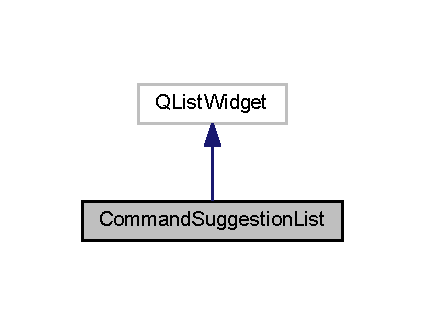
\includegraphics[width=204pt]{class_command_suggestion_list__inherit__graph}
\end{center}
\end{figure}


Collaboration diagram for Command\-Suggestion\-List\-:\nopagebreak
\begin{figure}[H]
\begin{center}
\leavevmode
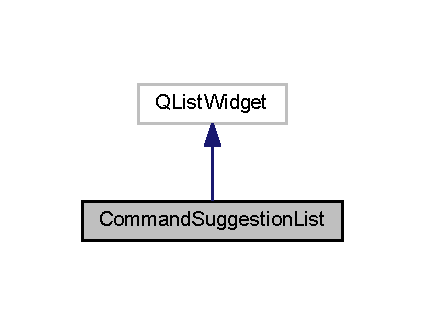
\includegraphics[width=204pt]{class_command_suggestion_list__coll__graph}
\end{center}
\end{figure}
\subsection*{Public Slots}
\begin{DoxyCompactItemize}
\item 
\hypertarget{class_command_suggestion_list_a8f033cd908b50fa9cc3383899f515943}{void \hyperlink{class_command_suggestion_list_a8f033cd908b50fa9cc3383899f515943}{move\-Up} ()}\label{class_command_suggestion_list_a8f033cd908b50fa9cc3383899f515943}

\begin{DoxyCompactList}\small\item\em Moves the selection up one item. \end{DoxyCompactList}\item 
\hypertarget{class_command_suggestion_list_a0df4ac65c3dc9db721b111d049330b64}{void \hyperlink{class_command_suggestion_list_a0df4ac65c3dc9db721b111d049330b64}{move\-Down} ()}\label{class_command_suggestion_list_a0df4ac65c3dc9db721b111d049330b64}

\begin{DoxyCompactList}\small\item\em Moves the selection up one item. \end{DoxyCompactList}\item 
\hypertarget{class_command_suggestion_list_abdfc24c738389f63440679e786328bb5}{void \hyperlink{class_command_suggestion_list_abdfc24c738389f63440679e786328bb5}{select\-First} ()}\label{class_command_suggestion_list_abdfc24c738389f63440679e786328bb5}

\begin{DoxyCompactList}\small\item\em Selects the first item. \end{DoxyCompactList}\item 
\hypertarget{class_command_suggestion_list_a5bbb5dc0289d336d123e852c0b4323c9}{void \hyperlink{class_command_suggestion_list_a5bbb5dc0289d336d123e852c0b4323c9}{auto\-Height} ()}\label{class_command_suggestion_list_a5bbb5dc0289d336d123e852c0b4323c9}

\begin{DoxyCompactList}\small\item\em Attempts to aut-\/size the suggestion box's height. \end{DoxyCompactList}\item 
\hypertarget{class_command_suggestion_list_a8b9a9ca017e2507b43fb55cd7e2584dd}{void \hyperlink{class_command_suggestion_list_a8b9a9ca017e2507b43fb55cd7e2584dd}{auto\-Width} ()}\label{class_command_suggestion_list_a8b9a9ca017e2507b43fb55cd7e2584dd}

\begin{DoxyCompactList}\small\item\em Attempts to aut-\/size the suggestion box's width. \end{DoxyCompactList}\end{DoxyCompactItemize}
\subsection*{Signals}
\begin{DoxyCompactItemize}
\item 
\hypertarget{class_command_suggestion_list_a9efae0883b3853d30dd5b94412c040de}{void \hyperlink{class_command_suggestion_list_a9efae0883b3853d30dd5b94412c040de}{height\-Scale\-Changed} ()}\label{class_command_suggestion_list_a9efae0883b3853d30dd5b94412c040de}

\begin{DoxyCompactList}\small\item\em Emitted when the height scale property is changed. \end{DoxyCompactList}\end{DoxyCompactItemize}
\subsection*{Public Member Functions}
\begin{DoxyCompactItemize}
\item 
\hyperlink{class_command_suggestion_list_aa6cd6f32861900fb5c0280375ee45969}{Command\-Suggestion\-List} (Q\-Widget $\ast$parent=0)
\begin{DoxyCompactList}\small\item\em Constructor. \end{DoxyCompactList}\item 
\hypertarget{class_command_suggestion_list_abc4ba5513dccfc66cddff8e028e73240}{virtual \hyperlink{class_command_suggestion_list_abc4ba5513dccfc66cddff8e028e73240}{$\sim$\-Command\-Suggestion\-List} ()}\label{class_command_suggestion_list_abc4ba5513dccfc66cddff8e028e73240}

\begin{DoxyCompactList}\small\item\em Destructor. \end{DoxyCompactList}\item 
Q\-String \hyperlink{class_command_suggestion_list_ae8f5411f7b8b3b4f86da8278951b448e}{get\-Current\-Selection} ()
\begin{DoxyCompactList}\small\item\em Returns a string representing the current selection. \end{DoxyCompactList}\item 
bool \hyperlink{class_command_suggestion_list_afc4dc846e366ece3bf77651fd92a7392}{has\-Selection} () const 
\begin{DoxyCompactList}\small\item\em Returns whether the suggestion box has a current selection. \end{DoxyCompactList}\item 
float \hyperlink{class_command_suggestion_list_a1430f35686d3572b51ebba9730083c97}{height\-Scale} () const 
\begin{DoxyCompactList}\small\item\em Gets the height scale for the suggestion box. \end{DoxyCompactList}\item 
void \hyperlink{class_command_suggestion_list_a5a05acbd3c0be81cb2fe7d2579cdb9a5}{set\-Height\-Scale} (float scale)
\begin{DoxyCompactList}\small\item\em Sets the height scale for the suggestion box. \end{DoxyCompactList}\item 
\hypertarget{class_command_suggestion_list_aedf54e67475b3d8e7ae116610de152a3}{void \hyperlink{class_command_suggestion_list_aedf54e67475b3d8e7ae116610de152a3}{reset\-Height\-Scale} ()}\label{class_command_suggestion_list_aedf54e67475b3d8e7ae116610de152a3}

\begin{DoxyCompactList}\small\item\em Resets the height scale to the default. \end{DoxyCompactList}\end{DoxyCompactItemize}
\subsection*{Properties}
\begin{DoxyCompactItemize}
\item 
float \hyperlink{class_command_suggestion_list_adb584feb5f08a036a35aa0ea1763e7b1}{height\-Scale}
\begin{DoxyCompactList}\small\item\em Scaling factor for height of suggestion box depending on how many items it contains. \end{DoxyCompactList}\end{DoxyCompactItemize}


\subsection{Detailed Description}
Holds and displays console command suggestions to the user. 

\subsection{Constructor \& Destructor Documentation}
\hypertarget{class_command_suggestion_list_aa6cd6f32861900fb5c0280375ee45969}{\index{Command\-Suggestion\-List@{Command\-Suggestion\-List}!Command\-Suggestion\-List@{Command\-Suggestion\-List}}
\index{Command\-Suggestion\-List@{Command\-Suggestion\-List}!CommandSuggestionList@{Command\-Suggestion\-List}}
\subsubsection[{Command\-Suggestion\-List}]{\setlength{\rightskip}{0pt plus 5cm}Command\-Suggestion\-List\-::\-Command\-Suggestion\-List (
\begin{DoxyParamCaption}
\item[{Q\-Widget $\ast$}]{parent = {\ttfamily 0}}
\end{DoxyParamCaption}
)\hspace{0.3cm}{\ttfamily [explicit]}}}\label{class_command_suggestion_list_aa6cd6f32861900fb5c0280375ee45969}


Constructor. 


\begin{DoxyParams}{Parameters}
{\em parent} & Q\-Widget parent, if applicable. \\
\hline
\end{DoxyParams}


\subsection{Member Function Documentation}
\hypertarget{class_command_suggestion_list_ae8f5411f7b8b3b4f86da8278951b448e}{\index{Command\-Suggestion\-List@{Command\-Suggestion\-List}!get\-Current\-Selection@{get\-Current\-Selection}}
\index{get\-Current\-Selection@{get\-Current\-Selection}!CommandSuggestionList@{Command\-Suggestion\-List}}
\subsubsection[{get\-Current\-Selection}]{\setlength{\rightskip}{0pt plus 5cm}Q\-String Command\-Suggestion\-List\-::get\-Current\-Selection (
\begin{DoxyParamCaption}
{}
\end{DoxyParamCaption}
)}}\label{class_command_suggestion_list_ae8f5411f7b8b3b4f86da8278951b448e}


Returns a string representing the current selection. 

\begin{DoxyReturn}{Returns}
Current selection string, or empty string if there is no selection. 
\end{DoxyReturn}
\hypertarget{class_command_suggestion_list_afc4dc846e366ece3bf77651fd92a7392}{\index{Command\-Suggestion\-List@{Command\-Suggestion\-List}!has\-Selection@{has\-Selection}}
\index{has\-Selection@{has\-Selection}!CommandSuggestionList@{Command\-Suggestion\-List}}
\subsubsection[{has\-Selection}]{\setlength{\rightskip}{0pt plus 5cm}bool Command\-Suggestion\-List\-::has\-Selection (
\begin{DoxyParamCaption}
{}
\end{DoxyParamCaption}
) const}}\label{class_command_suggestion_list_afc4dc846e366ece3bf77651fd92a7392}


Returns whether the suggestion box has a current selection. 

\begin{DoxyReturn}{Returns}
True if an item is selected, false otherwise. 
\end{DoxyReturn}
\hypertarget{class_command_suggestion_list_a1430f35686d3572b51ebba9730083c97}{\index{Command\-Suggestion\-List@{Command\-Suggestion\-List}!height\-Scale@{height\-Scale}}
\index{height\-Scale@{height\-Scale}!CommandSuggestionList@{Command\-Suggestion\-List}}
\subsubsection[{height\-Scale}]{\setlength{\rightskip}{0pt plus 5cm}float Command\-Suggestion\-List\-::height\-Scale (
\begin{DoxyParamCaption}
{}
\end{DoxyParamCaption}
) const}}\label{class_command_suggestion_list_a1430f35686d3572b51ebba9730083c97}


Gets the height scale for the suggestion box. 

\begin{DoxyReturn}{Returns}
Height scale. 
\end{DoxyReturn}
\hypertarget{class_command_suggestion_list_a5a05acbd3c0be81cb2fe7d2579cdb9a5}{\index{Command\-Suggestion\-List@{Command\-Suggestion\-List}!set\-Height\-Scale@{set\-Height\-Scale}}
\index{set\-Height\-Scale@{set\-Height\-Scale}!CommandSuggestionList@{Command\-Suggestion\-List}}
\subsubsection[{set\-Height\-Scale}]{\setlength{\rightskip}{0pt plus 5cm}void Command\-Suggestion\-List\-::set\-Height\-Scale (
\begin{DoxyParamCaption}
\item[{float}]{scale}
\end{DoxyParamCaption}
)}}\label{class_command_suggestion_list_a5a05acbd3c0be81cb2fe7d2579cdb9a5}


Sets the height scale for the suggestion box. 


\begin{DoxyParams}{Parameters}
{\em scale} & Scale to set. \\
\hline
\end{DoxyParams}


\subsection{Property Documentation}
\hypertarget{class_command_suggestion_list_adb584feb5f08a036a35aa0ea1763e7b1}{\index{Command\-Suggestion\-List@{Command\-Suggestion\-List}!height\-Scale@{height\-Scale}}
\index{height\-Scale@{height\-Scale}!CommandSuggestionList@{Command\-Suggestion\-List}}
\subsubsection[{height\-Scale}]{\setlength{\rightskip}{0pt plus 5cm}float Command\-Suggestion\-List\-::height\-Scale\hspace{0.3cm}{\ttfamily [read]}, {\ttfamily [write]}}}\label{class_command_suggestion_list_adb584feb5f08a036a35aa0ea1763e7b1}


Scaling factor for height of suggestion box depending on how many items it contains. 

\begin{DoxyParagraph}{Accessors\-:}
\hyperlink{class_command_suggestion_list_adb584feb5f08a036a35aa0ea1763e7b1}{height\-Scale()}, \hyperlink{class_command_suggestion_list_a5a05acbd3c0be81cb2fe7d2579cdb9a5}{set\-Height\-Scale()}, \hyperlink{class_command_suggestion_list_aedf54e67475b3d8e7ae116610de152a3}{reset\-Height\-Scale()}, \hyperlink{class_command_suggestion_list_a9efae0883b3853d30dd5b94412c040de}{height\-Scale\-Changed()} 
\end{DoxyParagraph}


The documentation for this class was generated from the following files\-:\begin{DoxyCompactItemize}
\item 
I\-Console/inc/\hyperlink{commandsuggestionlist_8h}{commandsuggestionlist.\-h}\item 
I\-Console/src/commandsuggestionlist.\-cpp\end{DoxyCompactItemize}

\hypertarget{class_con_command}{\section{Con\-Command Class Reference}
\label{class_con_command}\index{Con\-Command@{Con\-Command}}
}


Defines code which is executed whenever the user enters the command name into the console.  




{\ttfamily \#include $<$concommand.\-h$>$}



Inheritance diagram for Con\-Command\-:\nopagebreak
\begin{figure}[H]
\begin{center}
\leavevmode
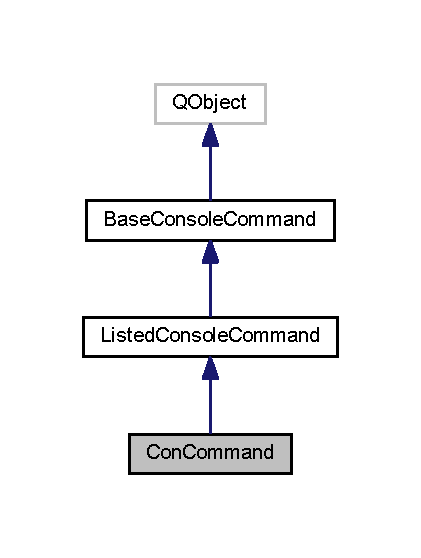
\includegraphics[width=202pt]{class_con_command__inherit__graph}
\end{center}
\end{figure}


Collaboration diagram for Con\-Command\-:\nopagebreak
\begin{figure}[H]
\begin{center}
\leavevmode
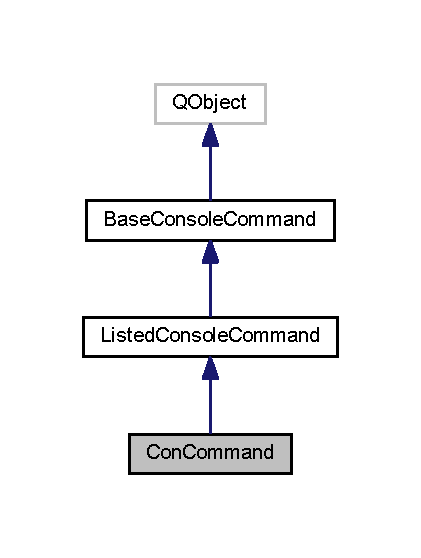
\includegraphics[width=202pt]{class_con_command__coll__graph}
\end{center}
\end{figure}
\subsection*{Public Member Functions}
\begin{DoxyCompactItemize}
\item 
\hyperlink{class_con_command_abd8a6c4780d77aa59f46233ac818e0e1}{Con\-Command} (const Q\-String \&\hyperlink{class_base_console_command_a2f21764f46a3864a362eae2e3396e363}{name}, N\-Global\-Cmd\-::\-Cmd\-Callback callback, const Q\-String \&desc=\char`\"{}\char`\"{}, N\-Global\-Cmd\-::\-C\-M\-D\-F\-L\-A\-G\-S flags=0, Q\-Object $\ast$parent=0)
\begin{DoxyCompactList}\small\item\em Constructor. \end{DoxyCompactList}\item 
\hyperlink{class_con_command_a8b048f3b99fdd95b2c4e26c2a0a117be}{Con\-Command} (const Q\-String \&\hyperlink{class_base_console_command_a2f21764f46a3864a362eae2e3396e363}{name}, N\-Global\-Cmd\-::\-Cmd\-Callback callback, \hyperlink{class_command_manager}{Command\-Manager} $\ast$manager, \hyperlink{class_listed_console_command}{Listed\-Console\-Command} $\ast$$\ast$list, const Q\-String \&desc=\char`\"{}\char`\"{}, const N\-Global\-Cmd\-::\-C\-M\-D\-F\-L\-A\-G\-S flags=0, Q\-Object $\ast$parent=0)
\begin{DoxyCompactList}\small\item\em Constructor passing in manager and list to attempt to register to. \end{DoxyCompactList}\item 
\hypertarget{class_con_command_a90b9ab62350b55966e959d88caa97c84}{virtual \hyperlink{class_con_command_a90b9ab62350b55966e959d88caa97c84}{$\sim$\-Con\-Command} ()}\label{class_con_command_a90b9ab62350b55966e959d88caa97c84}

\begin{DoxyCompactList}\small\item\em Destructor. \end{DoxyCompactList}\item 
virtual N\-Global\-Cmd\-::\-Cmd\-Ident \hyperlink{class_con_command_ab287443a9615df46739d0c39b096016e}{identify} () const 
\begin{DoxyCompactList}\small\item\em Returns the identifier for this command. \end{DoxyCompactList}\item 
int \hyperlink{class_con_command_af6d7e9c4e0b654f0b3e9a34cb5b22179}{exec} (const \hyperlink{class_command_sender_info}{Command\-Sender\-Info} \&info, const Q\-String\-List \&args, Q\-Variant \&output)
\begin{DoxyCompactList}\small\item\em Runs the console command's execution function. \end{DoxyCompactList}\item 
N\-Global\-Cmd\-::\-Cmd\-Callback \hyperlink{class_con_command_a7ff5a03d8a8a6ab7badaef4ffd083714}{get\-Exec} () const 
\begin{DoxyCompactList}\small\item\em Gets the callback function pointer for this console command. \end{DoxyCompactList}\item 
void \hyperlink{class_con_command_a3ae23385874e68d3e72ef50d0baf2ade}{set\-Exec} (N\-Global\-Cmd\-::\-Cmd\-Callback cmd)
\begin{DoxyCompactList}\small\item\em Sets the callback function that is run when this command is executed. \end{DoxyCompactList}\item 
virtual void \hyperlink{class_con_command_a87828b1909270309d2005a03ca2cd413}{set\-Flags\-Raw} (N\-Global\-Cmd\-::\-C\-M\-D\-F\-L\-A\-G\-S flags)
\begin{DoxyCompactList}\small\item\em Overwrites all flags on the command. \end{DoxyCompactList}\item 
virtual void \hyperlink{class_con_command_a7004e0c6eb421e5dfb90bd633e85bf14}{set\-Flag} (N\-Global\-Cmd\-::\-C\-M\-D\-F\-L\-A\-G\-S flag)
\begin{DoxyCompactList}\small\item\em Sets the given flag(s) on the command. \end{DoxyCompactList}\item 
virtual void \hyperlink{class_con_command_ab2591a1c31847e9746520e9958ba0f9a}{toggle\-Flag} (N\-Global\-Cmd\-::\-C\-M\-D\-F\-L\-A\-G\-S flag)
\begin{DoxyCompactList}\small\item\em Toggles the given flag(s) on the command. \end{DoxyCompactList}\end{DoxyCompactItemize}
\subsection*{Additional Inherited Members}


\subsection{Detailed Description}
Defines code which is executed whenever the user enters the command name into the console. 

Con\-Commands work almost exactly the same way as in the Source engine\-: they contain a pointer to a method which is executed when the command is typed by the user. When a \hyperlink{class_con_command}{Con\-Command} is executed, it returns an integer status (usually corresponding to an N\-Global\-Cmd\-::\-Con\-Command\-Return value) and can optionally return arbitrary output in the output Q\-Variant. Con\-Commands can write output to the a console window (relevant to the calling \hyperlink{class_command_manager}{Command\-Manager}, if one exists) through the passed \hyperlink{class_command_sender_info}{Command\-Sender\-Info}. 

\subsection{Constructor \& Destructor Documentation}
\hypertarget{class_con_command_abd8a6c4780d77aa59f46233ac818e0e1}{\index{Con\-Command@{Con\-Command}!Con\-Command@{Con\-Command}}
\index{Con\-Command@{Con\-Command}!ConCommand@{Con\-Command}}
\subsubsection[{Con\-Command}]{\setlength{\rightskip}{0pt plus 5cm}Con\-Command\-::\-Con\-Command (
\begin{DoxyParamCaption}
\item[{const Q\-String \&}]{name, }
\item[{N\-Global\-Cmd\-::\-Cmd\-Callback}]{callback, }
\item[{const Q\-String \&}]{desc = {\ttfamily \char`\"{}\char`\"{}}, }
\item[{N\-Global\-Cmd\-::\-C\-M\-D\-F\-L\-A\-G\-S}]{flags = {\ttfamily 0}, }
\item[{Q\-Object $\ast$}]{parent = {\ttfamily 0}}
\end{DoxyParamCaption}
)\hspace{0.3cm}{\ttfamily [explicit]}}}\label{class_con_command_abd8a6c4780d77aa59f46233ac818e0e1}


Constructor. 


\begin{DoxyParams}{Parameters}
{\em name} & Name of the command. \\
\hline
{\em callback} & Pointer to callback function to run when this command is executed. \\
\hline
{\em desc} & Optional command description. \\
\hline
{\em flags} & Command flags. \\
\hline
{\em parent} & Q\-Object parent, if applicable. \\
\hline
\end{DoxyParams}
\hypertarget{class_con_command_a8b048f3b99fdd95b2c4e26c2a0a117be}{\index{Con\-Command@{Con\-Command}!Con\-Command@{Con\-Command}}
\index{Con\-Command@{Con\-Command}!ConCommand@{Con\-Command}}
\subsubsection[{Con\-Command}]{\setlength{\rightskip}{0pt plus 5cm}Con\-Command\-::\-Con\-Command (
\begin{DoxyParamCaption}
\item[{const Q\-String \&}]{name, }
\item[{N\-Global\-Cmd\-::\-Cmd\-Callback}]{callback, }
\item[{{\bf Command\-Manager} $\ast$}]{manager, }
\item[{{\bf Listed\-Console\-Command} $\ast$$\ast$}]{list, }
\item[{const Q\-String \&}]{desc = {\ttfamily \char`\"{}\char`\"{}}, }
\item[{const N\-Global\-Cmd\-::\-C\-M\-D\-F\-L\-A\-G\-S}]{flags = {\ttfamily 0}, }
\item[{Q\-Object $\ast$}]{parent = {\ttfamily 0}}
\end{DoxyParamCaption}
)\hspace{0.3cm}{\ttfamily [explicit]}}}\label{class_con_command_a8b048f3b99fdd95b2c4e26c2a0a117be}


Constructor passing in manager and list to attempt to register to. 


\begin{DoxyParams}{Parameters}
{\em name} & Name of the command. \\
\hline
{\em callback} & Pointer to callback function to run when this command is executed. \\
\hline
{\em manager} & Manager to attempt to register to when this command is constructed. \\
\hline
{\em list} & If the command could not register with the manager, it attaches itself to this list instead. \\
\hline
{\em desc} & Optional command description. \\
\hline
{\em flags} & Command flags. \\
\hline
{\em parent} & Q\-Object parent, if applicable. \\
\hline
\end{DoxyParams}


\subsection{Member Function Documentation}
\hypertarget{class_con_command_af6d7e9c4e0b654f0b3e9a34cb5b22179}{\index{Con\-Command@{Con\-Command}!exec@{exec}}
\index{exec@{exec}!ConCommand@{Con\-Command}}
\subsubsection[{exec}]{\setlength{\rightskip}{0pt plus 5cm}int Con\-Command\-::exec (
\begin{DoxyParamCaption}
\item[{const {\bf Command\-Sender\-Info} \&}]{info, }
\item[{const Q\-String\-List \&}]{args, }
\item[{Q\-Variant \&}]{output}
\end{DoxyParamCaption}
)}}\label{class_con_command_af6d7e9c4e0b654f0b3e9a34cb5b22179}


Runs the console command's execution function. 


\begin{DoxyParams}{Parameters}
{\em info} & Info class to facilitate communication between the command and the caller. \\
\hline
{\em args} & Arguments to the command. \\
\hline
{\em output} & Q\-Variant to hold any output from the command. \\
\hline
\end{DoxyParams}
\begin{DoxyReturn}{Returns}
Integer return code of the command function. 
\end{DoxyReturn}
\hypertarget{class_con_command_a7ff5a03d8a8a6ab7badaef4ffd083714}{\index{Con\-Command@{Con\-Command}!get\-Exec@{get\-Exec}}
\index{get\-Exec@{get\-Exec}!ConCommand@{Con\-Command}}
\subsubsection[{get\-Exec}]{\setlength{\rightskip}{0pt plus 5cm}N\-Global\-Cmd\-::\-Cmd\-Callback Con\-Command\-::get\-Exec (
\begin{DoxyParamCaption}
{}
\end{DoxyParamCaption}
) const}}\label{class_con_command_a7ff5a03d8a8a6ab7badaef4ffd083714}


Gets the callback function pointer for this console command. 

\begin{DoxyReturn}{Returns}
Pointer to callback function to run when this command is executed. 
\end{DoxyReturn}
\hypertarget{class_con_command_ab287443a9615df46739d0c39b096016e}{\index{Con\-Command@{Con\-Command}!identify@{identify}}
\index{identify@{identify}!ConCommand@{Con\-Command}}
\subsubsection[{identify}]{\setlength{\rightskip}{0pt plus 5cm}N\-Global\-Cmd\-::\-Cmd\-Ident Con\-Command\-::identify (
\begin{DoxyParamCaption}
{}
\end{DoxyParamCaption}
) const\hspace{0.3cm}{\ttfamily [virtual]}}}\label{class_con_command_ab287443a9615df46739d0c39b096016e}


Returns the identifier for this command. 

\begin{DoxyReturn}{Returns}
Cmd\-Ident\-::\-C\-I\-Command for console commands. 
\end{DoxyReturn}


Reimplemented from \hyperlink{class_base_console_command_a8c1fe488f1e24c6bd4891225eb9bb122}{Base\-Console\-Command}.

\hypertarget{class_con_command_a3ae23385874e68d3e72ef50d0baf2ade}{\index{Con\-Command@{Con\-Command}!set\-Exec@{set\-Exec}}
\index{set\-Exec@{set\-Exec}!ConCommand@{Con\-Command}}
\subsubsection[{set\-Exec}]{\setlength{\rightskip}{0pt plus 5cm}void Con\-Command\-::set\-Exec (
\begin{DoxyParamCaption}
\item[{N\-Global\-Cmd\-::\-Cmd\-Callback}]{cmd}
\end{DoxyParamCaption}
)}}\label{class_con_command_a3ae23385874e68d3e72ef50d0baf2ade}


Sets the callback function that is run when this command is executed. 


\begin{DoxyParams}{Parameters}
{\em cmd} & Pointer to callback. \\
\hline
\end{DoxyParams}
\hypertarget{class_con_command_a7004e0c6eb421e5dfb90bd633e85bf14}{\index{Con\-Command@{Con\-Command}!set\-Flag@{set\-Flag}}
\index{set\-Flag@{set\-Flag}!ConCommand@{Con\-Command}}
\subsubsection[{set\-Flag}]{\setlength{\rightskip}{0pt plus 5cm}void Con\-Command\-::set\-Flag (
\begin{DoxyParamCaption}
\item[{N\-Global\-Cmd\-::\-C\-M\-D\-F\-L\-A\-G\-S}]{flag}
\end{DoxyParamCaption}
)\hspace{0.3cm}{\ttfamily [virtual]}}}\label{class_con_command_a7004e0c6eb421e5dfb90bd633e85bf14}


Sets the given flag(s) on the command. 


\begin{DoxyParams}{Parameters}
{\em flag} & Flag(s) to set. \\
\hline
\end{DoxyParams}


Reimplemented from \hyperlink{class_base_console_command_a3046da732d30b1de8b41f51d146b5e46}{Base\-Console\-Command}.

\hypertarget{class_con_command_a87828b1909270309d2005a03ca2cd413}{\index{Con\-Command@{Con\-Command}!set\-Flags\-Raw@{set\-Flags\-Raw}}
\index{set\-Flags\-Raw@{set\-Flags\-Raw}!ConCommand@{Con\-Command}}
\subsubsection[{set\-Flags\-Raw}]{\setlength{\rightskip}{0pt plus 5cm}void Con\-Command\-::set\-Flags\-Raw (
\begin{DoxyParamCaption}
\item[{N\-Global\-Cmd\-::\-C\-M\-D\-F\-L\-A\-G\-S}]{flags}
\end{DoxyParamCaption}
)\hspace{0.3cm}{\ttfamily [virtual]}}}\label{class_con_command_a87828b1909270309d2005a03ca2cd413}


Overwrites all flags on the command. 


\begin{DoxyParams}{Parameters}
{\em flags} & Integer containing the exact state of all flags to set. \\
\hline
\end{DoxyParams}


Reimplemented from \hyperlink{class_base_console_command_ac6ff6169ab06ae43d76d0b3c2e5336ff}{Base\-Console\-Command}.

\hypertarget{class_con_command_ab2591a1c31847e9746520e9958ba0f9a}{\index{Con\-Command@{Con\-Command}!toggle\-Flag@{toggle\-Flag}}
\index{toggle\-Flag@{toggle\-Flag}!ConCommand@{Con\-Command}}
\subsubsection[{toggle\-Flag}]{\setlength{\rightskip}{0pt plus 5cm}void Con\-Command\-::toggle\-Flag (
\begin{DoxyParamCaption}
\item[{N\-Global\-Cmd\-::\-C\-M\-D\-F\-L\-A\-G\-S}]{flag}
\end{DoxyParamCaption}
)\hspace{0.3cm}{\ttfamily [virtual]}}}\label{class_con_command_ab2591a1c31847e9746520e9958ba0f9a}


Toggles the given flag(s) on the command. 


\begin{DoxyParams}{Parameters}
{\em flag} & Flag(s) to toggle. \\
\hline
\end{DoxyParams}


Reimplemented from \hyperlink{class_base_console_command_a509caa8e6fba5c10e9ff89dd5fb665cf}{Base\-Console\-Command}.



The documentation for this class was generated from the following files\-:\begin{DoxyCompactItemize}
\item 
I\-Console/inc/\hyperlink{concommand_8h}{concommand.\-h}\item 
I\-Console/src/concommand.\-cpp\end{DoxyCompactItemize}

\hypertarget{class_console_widget}{\section{Console\-Widget Class Reference}
\label{class_console_widget}\index{Console\-Widget@{Console\-Widget}}
}


Inheritance diagram for Console\-Widget\-:\nopagebreak
\begin{figure}[H]
\begin{center}
\leavevmode
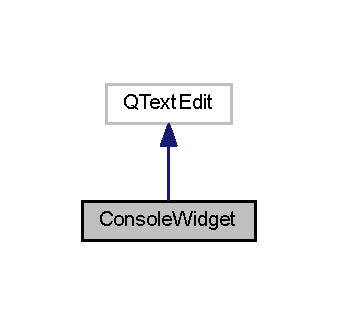
\includegraphics[width=162pt]{class_console_widget__inherit__graph}
\end{center}
\end{figure}


Collaboration diagram for Console\-Widget\-:\nopagebreak
\begin{figure}[H]
\begin{center}
\leavevmode
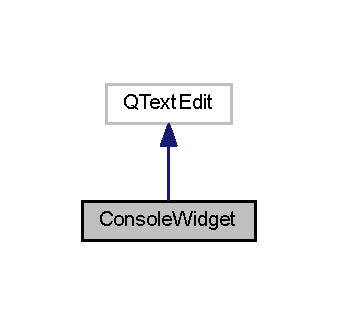
\includegraphics[width=162pt]{class_console_widget__coll__graph}
\end{center}
\end{figure}
\subsection*{Public Slots}
\begin{DoxyCompactItemize}
\item 
\hypertarget{class_console_widget_a04e2902e857852f3185c74de71ae3c9b}{void {\bfseries print\-Message} (const Q\-String \&message)}\label{class_console_widget_a04e2902e857852f3185c74de71ae3c9b}

\item 
\hypertarget{class_console_widget_adef216de346ef5f08f38c0874777167b}{void {\bfseries print\-Warning} (const Q\-String \&message)}\label{class_console_widget_adef216de346ef5f08f38c0874777167b}

\item 
\hypertarget{class_console_widget_a9f7957ef32ab4e68a58b0cbcf1c07c89}{void {\bfseries print\-Message} (\hyperlink{class_command_sender_info_a3a5e6a2ef1772f6557f351652c2e3b60}{Command\-Sender\-Info\-::\-Output\-Type} type, const Q\-String \&message)}\label{class_console_widget_a9f7957ef32ab4e68a58b0cbcf1c07c89}

\item 
\hypertarget{class_console_widget_ab079b67c769e850d451ad3fdbbbdc750}{void {\bfseries repolish} ()}\label{class_console_widget_ab079b67c769e850d451ad3fdbbbdc750}

\end{DoxyCompactItemize}
\subsection*{Signals}
\begin{DoxyCompactItemize}
\item 
\hypertarget{class_console_widget_ad8c0d1aba62d12986b8ec8faeff1a2ae}{void {\bfseries max\-Lines\-Changed} ()}\label{class_console_widget_ad8c0d1aba62d12986b8ec8faeff1a2ae}

\item 
\hypertarget{class_console_widget_a51d0bb1f81c3c8dff9788f5dbf03b569}{void {\bfseries message\-Color\-Changed} ()}\label{class_console_widget_a51d0bb1f81c3c8dff9788f5dbf03b569}

\item 
\hypertarget{class_console_widget_a10b823a6b68216c362f75ed01d5fae81}{void {\bfseries warning\-Color\-Changed} ()}\label{class_console_widget_a10b823a6b68216c362f75ed01d5fae81}

\item 
\hypertarget{class_console_widget_aa28f784431c1fcb257ca607abf482741}{void {\bfseries custom\-Color1\-Changed} ()}\label{class_console_widget_aa28f784431c1fcb257ca607abf482741}

\item 
\hypertarget{class_console_widget_abe4b076d1edab52e276659a6ae55bdc5}{void {\bfseries custom\-Color2\-Changed} ()}\label{class_console_widget_abe4b076d1edab52e276659a6ae55bdc5}

\item 
\hypertarget{class_console_widget_a0eece2c8ac4de3639931b76e82c08196}{void {\bfseries custom\-Color3\-Changed} ()}\label{class_console_widget_a0eece2c8ac4de3639931b76e82c08196}

\item 
\hypertarget{class_console_widget_a655f6522aa4bbfc625c3d6f9ffbfe26e}{void {\bfseries custom\-Color4\-Changed} ()}\label{class_console_widget_a655f6522aa4bbfc625c3d6f9ffbfe26e}

\item 
\hypertarget{class_console_widget_a1d2c4dee435697402c0e4b482bd051bc}{void {\bfseries custom\-Color5\-Changed} ()}\label{class_console_widget_a1d2c4dee435697402c0e4b482bd051bc}

\item 
\hypertarget{class_console_widget_a8f9b8bb7e73504bbbd80b07cb36381cb}{void {\bfseries custom\-Color6\-Changed} ()}\label{class_console_widget_a8f9b8bb7e73504bbbd80b07cb36381cb}

\end{DoxyCompactItemize}
\subsection*{Public Member Functions}
\begin{DoxyCompactItemize}
\item 
\hypertarget{class_console_widget_a4a66caaf3f7583a46ebe44a5c2221160}{{\bfseries Console\-Widget} (Q\-Widget $\ast$parent=0)}\label{class_console_widget_a4a66caaf3f7583a46ebe44a5c2221160}

\item 
\hypertarget{class_console_widget_a1e01a4e339ff6781cbfec5bd59c292f6}{int {\bfseries max\-Lines} () const }\label{class_console_widget_a1e01a4e339ff6781cbfec5bd59c292f6}

\item 
\hypertarget{class_console_widget_a5bb26af5e53e3025d31b40d8e284feb9}{void {\bfseries set\-Max\-Lines} (int lines)}\label{class_console_widget_a5bb26af5e53e3025d31b40d8e284feb9}

\item 
\hypertarget{class_console_widget_a58291752b182ad84572e36029c42e827}{void {\bfseries reset\-Max\-Lines} ()}\label{class_console_widget_a58291752b182ad84572e36029c42e827}

\item 
\hypertarget{class_console_widget_af9dfb729ec2a6973880d717d5b9c1c78}{Q\-Color {\bfseries message\-Color} () const }\label{class_console_widget_af9dfb729ec2a6973880d717d5b9c1c78}

\item 
\hypertarget{class_console_widget_a290f1f7d09a6fb2078cada80d6e8024c}{void {\bfseries set\-Message\-Color} (Q\-Color col)}\label{class_console_widget_a290f1f7d09a6fb2078cada80d6e8024c}

\item 
\hypertarget{class_console_widget_a899d2b558ccf3976e45514fd4bd9eb7c}{void {\bfseries reset\-Message\-Color} ()}\label{class_console_widget_a899d2b558ccf3976e45514fd4bd9eb7c}

\item 
\hypertarget{class_console_widget_af1abcb3bb2a6be074233e1891ecace91}{Q\-Color {\bfseries warning\-Color} () const }\label{class_console_widget_af1abcb3bb2a6be074233e1891ecace91}

\item 
\hypertarget{class_console_widget_aaf8789dc58ae736b951552b1fb9cef0d}{void {\bfseries set\-Warning\-Color} (Q\-Color col)}\label{class_console_widget_aaf8789dc58ae736b951552b1fb9cef0d}

\item 
\hypertarget{class_console_widget_af089740931bec97455b7858afc0d291c}{void {\bfseries reset\-Warning\-Color} ()}\label{class_console_widget_af089740931bec97455b7858afc0d291c}

\item 
\hypertarget{class_console_widget_a07e085ea01f992aa1de72937dba48fb2}{Q\-Color {\bfseries custom\-Color1} () const }\label{class_console_widget_a07e085ea01f992aa1de72937dba48fb2}

\item 
\hypertarget{class_console_widget_a4317870d3883d218a297f2d0b2a10a06}{Q\-Color {\bfseries custom\-Color2} () const }\label{class_console_widget_a4317870d3883d218a297f2d0b2a10a06}

\item 
\hypertarget{class_console_widget_a50faf85bc735a6ce59222eb2f229c7c5}{Q\-Color {\bfseries custom\-Color3} () const }\label{class_console_widget_a50faf85bc735a6ce59222eb2f229c7c5}

\item 
\hypertarget{class_console_widget_a7acd9d9d522e5add2107befebf86a839}{Q\-Color {\bfseries custom\-Color4} () const }\label{class_console_widget_a7acd9d9d522e5add2107befebf86a839}

\item 
\hypertarget{class_console_widget_a57756fc88c1196455c2afa370556a71d}{Q\-Color {\bfseries custom\-Color5} () const }\label{class_console_widget_a57756fc88c1196455c2afa370556a71d}

\item 
\hypertarget{class_console_widget_ac5e34f19cc36cdd4b4dac3566c2eaf64}{Q\-Color {\bfseries custom\-Color6} () const }\label{class_console_widget_ac5e34f19cc36cdd4b4dac3566c2eaf64}

\item 
\hypertarget{class_console_widget_a509414a25aabbf38167a8f1d57fea09c}{void {\bfseries set\-Custom\-Color1} (Q\-Color col)}\label{class_console_widget_a509414a25aabbf38167a8f1d57fea09c}

\item 
\hypertarget{class_console_widget_a14e6815763803393376f4fd1db78821e}{void {\bfseries set\-Custom\-Color2} (Q\-Color col)}\label{class_console_widget_a14e6815763803393376f4fd1db78821e}

\item 
\hypertarget{class_console_widget_aed0c8abe6d9b92aef97266e2b93b347f}{void {\bfseries set\-Custom\-Color3} (Q\-Color col)}\label{class_console_widget_aed0c8abe6d9b92aef97266e2b93b347f}

\item 
\hypertarget{class_console_widget_ae10358d0184634959dd97e65e19bd9ef}{void {\bfseries set\-Custom\-Color4} (Q\-Color col)}\label{class_console_widget_ae10358d0184634959dd97e65e19bd9ef}

\item 
\hypertarget{class_console_widget_a361194a1e900563462e7639331e1fb4c}{void {\bfseries set\-Custom\-Color5} (Q\-Color col)}\label{class_console_widget_a361194a1e900563462e7639331e1fb4c}

\item 
\hypertarget{class_console_widget_a6ce29c64f664955b37065c7ba84bfd00}{void {\bfseries set\-Custom\-Color6} (Q\-Color col)}\label{class_console_widget_a6ce29c64f664955b37065c7ba84bfd00}

\item 
\hypertarget{class_console_widget_a2097aef6f449a6d2dd5f653623801f80}{void {\bfseries reset\-Custom\-Color1} ()}\label{class_console_widget_a2097aef6f449a6d2dd5f653623801f80}

\item 
\hypertarget{class_console_widget_ab3061f5106972084d70bffe9dfffb007}{void {\bfseries reset\-Custom\-Color2} ()}\label{class_console_widget_ab3061f5106972084d70bffe9dfffb007}

\item 
\hypertarget{class_console_widget_acdb81d6a8a21fcb15ebbf3c0cefcd434}{void {\bfseries reset\-Custom\-Color3} ()}\label{class_console_widget_acdb81d6a8a21fcb15ebbf3c0cefcd434}

\item 
\hypertarget{class_console_widget_ac955271b9857a7f7e1a23d25a6c9082d}{void {\bfseries reset\-Custom\-Color4} ()}\label{class_console_widget_ac955271b9857a7f7e1a23d25a6c9082d}

\item 
\hypertarget{class_console_widget_a30cf8697ccef1adbd6b21a91ca4aceb1}{void {\bfseries reset\-Custom\-Color5} ()}\label{class_console_widget_a30cf8697ccef1adbd6b21a91ca4aceb1}

\item 
\hypertarget{class_console_widget_a2e8fe2f9d7e27f923294a93be8c4f702}{void {\bfseries reset\-Custom\-Color6} ()}\label{class_console_widget_a2e8fe2f9d7e27f923294a93be8c4f702}

\end{DoxyCompactItemize}
\subsection*{Static Public Attributes}
\begin{DoxyCompactItemize}
\item 
\hypertarget{class_console_widget_af215d1c2ed6a4b8891528dd0cdbc4585}{static const unsigned int {\bfseries D\-E\-F\-A\-U\-L\-T\-\_\-\-M\-A\-X\-\_\-\-L\-I\-N\-E\-S} = 256}\label{class_console_widget_af215d1c2ed6a4b8891528dd0cdbc4585}

\item 
\hypertarget{class_console_widget_a1b1a4275424776cca6958cc5afd3c2d1}{static const Q\-Color {\bfseries D\-E\-F\-A\-U\-L\-T\-\_\-\-M\-E\-S\-S\-A\-G\-E\-\_\-\-C\-O\-L\-O\-U\-R} = Q\-Color(0,0,0)}\label{class_console_widget_a1b1a4275424776cca6958cc5afd3c2d1}

\item 
\hypertarget{class_console_widget_ab73a773298b4822640c9a64c9f75b8a8}{static const Q\-Color {\bfseries D\-E\-F\-A\-U\-L\-T\-\_\-\-W\-A\-R\-N\-I\-N\-G\-\_\-\-C\-O\-L\-O\-U\-R} = Q\-Color(255,0,0)}\label{class_console_widget_ab73a773298b4822640c9a64c9f75b8a8}

\item 
\hypertarget{class_console_widget_abbd61319fc0c7feeb51623498eddeb9a}{static const Q\-Color {\bfseries D\-E\-F\-A\-U\-L\-T\-\_\-\-C\-U\-S\-T\-O\-M\-\_\-\-C\-O\-L\-O\-U\-R1} = Q\-Color(208,208,208)}\label{class_console_widget_abbd61319fc0c7feeb51623498eddeb9a}

\item 
\hypertarget{class_console_widget_a07ff3055aa08dd9d86531db2838e086a}{static const Q\-Color {\bfseries D\-E\-F\-A\-U\-L\-T\-\_\-\-C\-U\-S\-T\-O\-M\-\_\-\-C\-O\-L\-O\-U\-R2} = Q\-Color(216,195,0)}\label{class_console_widget_a07ff3055aa08dd9d86531db2838e086a}

\item 
\hypertarget{class_console_widget_a5c08a0f2b6fa95efdc7c86b79d70c126}{static const Q\-Color {\bfseries D\-E\-F\-A\-U\-L\-T\-\_\-\-C\-U\-S\-T\-O\-M\-\_\-\-C\-O\-L\-O\-U\-R3} = Q\-Color(255,106,43)}\label{class_console_widget_a5c08a0f2b6fa95efdc7c86b79d70c126}

\item 
\hypertarget{class_console_widget_a82acbc07440b3d74150fe7d72279ae2b}{static const Q\-Color {\bfseries D\-E\-F\-A\-U\-L\-T\-\_\-\-C\-U\-S\-T\-O\-M\-\_\-\-C\-O\-L\-O\-U\-R4} = Q\-Color(255,0,255)}\label{class_console_widget_a82acbc07440b3d74150fe7d72279ae2b}

\item 
\hypertarget{class_console_widget_aad9ca0556290f9d68e01f13390acee04}{static const Q\-Color {\bfseries D\-E\-F\-A\-U\-L\-T\-\_\-\-C\-U\-S\-T\-O\-M\-\_\-\-C\-O\-L\-O\-U\-R5} = Q\-Color(0,255,255)}\label{class_console_widget_aad9ca0556290f9d68e01f13390acee04}

\item 
\hypertarget{class_console_widget_a29de764d1511c834b28247784a115b4d}{static const Q\-Color {\bfseries D\-E\-F\-A\-U\-L\-T\-\_\-\-C\-U\-S\-T\-O\-M\-\_\-\-C\-O\-L\-O\-U\-R6} = Q\-Color(0,255,0)}\label{class_console_widget_a29de764d1511c834b28247784a115b4d}

\end{DoxyCompactItemize}
\subsection*{Properties}
\begin{DoxyCompactItemize}
\item 
\hypertarget{class_console_widget_afef59d721756f56c09780682aa0e7fac}{int {\bfseries max\-Lines}}\label{class_console_widget_afef59d721756f56c09780682aa0e7fac}

\item 
\hypertarget{class_console_widget_a2c801d4bdb2605d0d4fcf2812b0f33fc}{Q\-Color {\bfseries message\-Color}}\label{class_console_widget_a2c801d4bdb2605d0d4fcf2812b0f33fc}

\item 
\hypertarget{class_console_widget_ac0fe2ed854169ca40a506eef06dd7627}{Q\-Color {\bfseries warning\-Color}}\label{class_console_widget_ac0fe2ed854169ca40a506eef06dd7627}

\item 
\hypertarget{class_console_widget_a2ced0beaf2345ea1a5a430dbecce8980}{Q\-Color {\bfseries custom\-Color1}}\label{class_console_widget_a2ced0beaf2345ea1a5a430dbecce8980}

\item 
\hypertarget{class_console_widget_a538953029512834275ace6ab1f9ff4f8}{Q\-Color {\bfseries custom\-Color2}}\label{class_console_widget_a538953029512834275ace6ab1f9ff4f8}

\item 
\hypertarget{class_console_widget_a3b0ddd26653c304ec53a0388a5b56ef7}{Q\-Color {\bfseries custom\-Color3}}\label{class_console_widget_a3b0ddd26653c304ec53a0388a5b56ef7}

\item 
\hypertarget{class_console_widget_aff88cf79de3c9d2f2679fe4729bd4e7b}{Q\-Color {\bfseries custom\-Color4}}\label{class_console_widget_aff88cf79de3c9d2f2679fe4729bd4e7b}

\item 
\hypertarget{class_console_widget_ae8282e6520cc5c909193c5f42bcba7f8}{Q\-Color {\bfseries custom\-Color5}}\label{class_console_widget_ae8282e6520cc5c909193c5f42bcba7f8}

\item 
\hypertarget{class_console_widget_a6f3957397a3eead2d5a7785342288239}{Q\-Color {\bfseries custom\-Color6}}\label{class_console_widget_a6f3957397a3eead2d5a7785342288239}

\end{DoxyCompactItemize}


The documentation for this class was generated from the following files\-:\begin{DoxyCompactItemize}
\item 
I\-Console/inc/consolewidget.\-h\item 
I\-Console/src/consolewidget.\-cpp\end{DoxyCompactItemize}

\hypertarget{class_console_window}{\section{Console\-Window Class Reference}
\label{class_console_window}\index{Console\-Window@{Console\-Window}}
}


Inheritance diagram for Console\-Window\-:
\nopagebreak
\begin{figure}[H]
\begin{center}
\leavevmode
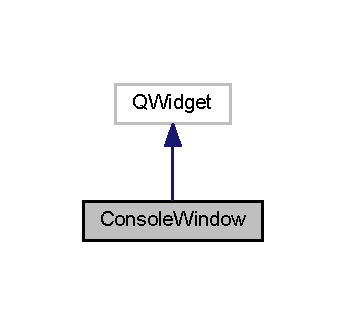
\includegraphics[width=247pt]{class_console_window__inherit__graph}
\end{center}
\end{figure}


Collaboration diagram for Console\-Window\-:
\nopagebreak
\begin{figure}[H]
\begin{center}
\leavevmode
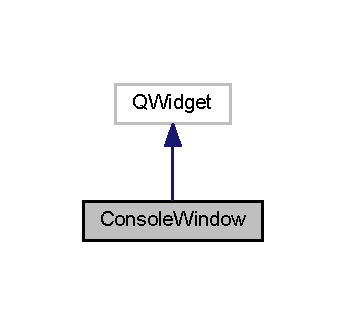
\includegraphics[width=247pt]{class_console_window__coll__graph}
\end{center}
\end{figure}
\subsection*{Public Slots}
\begin{DoxyCompactItemize}
\item 
\hypertarget{class_console_window_ae9c69bfdddc7e06686ce1aef07228a5f}{void {\bfseries slot\-Print\-Message} (const Q\-String \&message)}\label{class_console_window_ae9c69bfdddc7e06686ce1aef07228a5f}

\item 
\hypertarget{class_console_window_a2a2390460eb7eae4ba129f3e649fa03e}{void {\bfseries slot\-Print\-Warning} (const Q\-String \&message)}\label{class_console_window_a2a2390460eb7eae4ba129f3e649fa03e}

\end{DoxyCompactItemize}
\subsection*{Public Member Functions}
\begin{DoxyCompactItemize}
\item 
\hypertarget{class_console_window_a18a5ddfb71f2bcec3a4ce8abee0863eb}{{\bfseries Console\-Window} (Q\-Widget $\ast$parent=0)}\label{class_console_window_a18a5ddfb71f2bcec3a4ce8abee0863eb}

\item 
\hypertarget{class_console_window_a92eb7fb004686e2659530d959080846e}{virtual void {\bfseries print\-Message} (const Q\-String \&message)}\label{class_console_window_a92eb7fb004686e2659530d959080846e}

\item 
\hypertarget{class_console_window_ab06d210a320e402b371dfa56d73f0d54}{virtual void {\bfseries print\-Warning} (const Q\-String \&message)}\label{class_console_window_ab06d210a320e402b371dfa56d73f0d54}

\item 
\hypertarget{class_console_window_a18dbd0234d103461b57da2b724ab5b2b}{void {\bfseries set\-Warning\-Colour} (const Q\-Color col)}\label{class_console_window_a18dbd0234d103461b57da2b724ab5b2b}

\item 
\hypertarget{class_console_window_afb123596c8c2e460301721dfe28b2642}{Q\-Color {\bfseries get\-Warning\-Colour} () const }\label{class_console_window_afb123596c8c2e460301721dfe28b2642}

\item 
\hypertarget{class_console_window_a92a66819f11ee2cb7ad6079bb0542562}{void {\bfseries set\-Message\-Colour} (const Q\-Color col)}\label{class_console_window_a92a66819f11ee2cb7ad6079bb0542562}

\item 
\hypertarget{class_console_window_a4deda073bdf749e5198ba48a41fef340}{Q\-Color {\bfseries get\-Message\-Colour} () const }\label{class_console_window_a4deda073bdf749e5198ba48a41fef340}

\end{DoxyCompactItemize}


The documentation for this class was generated from the following files\-:\begin{DoxyCompactItemize}
\item 
I\-Console/consolewindow.\-h\item 
I\-Console/consolewindow.\-cpp\end{DoxyCompactItemize}

\hypertarget{class_con_var}{\section{Con\-Var Class Reference}
\label{class_con_var}\index{Con\-Var@{Con\-Var}}
}


Stores values that are retrievable and settable by the user (from the console) or by the application (via code).  




{\ttfamily \#include $<$convar.\-h$>$}



Inheritance diagram for Con\-Var\-:\nopagebreak
\begin{figure}[H]
\begin{center}
\leavevmode
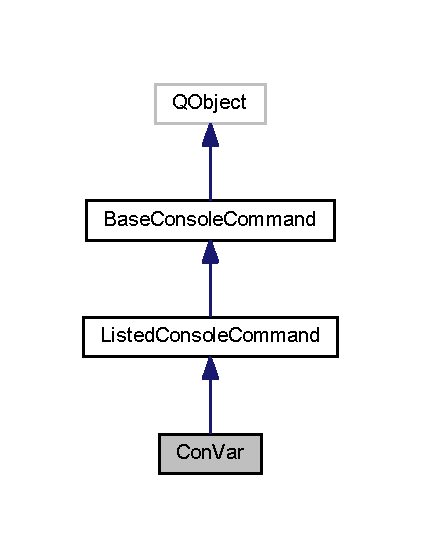
\includegraphics[width=202pt]{class_con_var__inherit__graph}
\end{center}
\end{figure}


Collaboration diagram for Con\-Var\-:\nopagebreak
\begin{figure}[H]
\begin{center}
\leavevmode
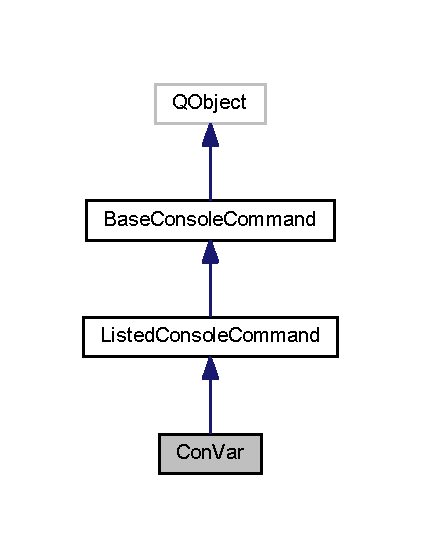
\includegraphics[width=202pt]{class_con_var__coll__graph}
\end{center}
\end{figure}
\subsection*{Public Member Functions}
\begin{DoxyCompactItemize}
\item 
\hyperlink{class_con_var_ac437fec999dde2751271c7c1e400d89d}{Con\-Var} (const Q\-String \&\hyperlink{class_base_console_command_a2f21764f46a3864a362eae2e3396e363}{name}, const Q\-String \&def, N\-Global\-Cmd\-::\-Var\-Callback callback=N\-U\-L\-L, const Q\-String \&desc=\char`\"{}\char`\"{}, N\-Global\-Cmd\-::\-C\-M\-D\-F\-L\-A\-G\-S flags=0, bool \hyperlink{class_con_var_a047d4105baf54cb783602456e0947196}{has\-Min}=false, float min=0.\-0, bool \hyperlink{class_con_var_ab8a0883ab2a53b5ef20ea5673636ac01}{has\-Max}=false, float max=0.\-0, Q\-Object $\ast$parent=0)
\begin{DoxyCompactList}\small\item\em Constructor. \end{DoxyCompactList}\item 
\hyperlink{class_con_var_a6755a812d1e97a6524c26a703e480359}{Con\-Var} (const Q\-String \&\hyperlink{class_base_console_command_a2f21764f46a3864a362eae2e3396e363}{name}, const Q\-String \&def, \hyperlink{class_command_manager}{Command\-Manager} $\ast$manager, \hyperlink{class_listed_console_command}{Listed\-Console\-Command} $\ast$$\ast$list, N\-Global\-Cmd\-::\-Var\-Callback callback=N\-U\-L\-L, const Q\-String \&desc=\char`\"{}\char`\"{}, N\-Global\-Cmd\-::\-C\-M\-D\-F\-L\-A\-G\-S flags=0, bool \hyperlink{class_con_var_a047d4105baf54cb783602456e0947196}{has\-Min}=false, float min=0.\-0f, bool has\-Max=false, float max=0.\-0f, Q\-Object $\ast$parent=0)
\begin{DoxyCompactList}\small\item\em Constructor. \end{DoxyCompactList}\item 
\hypertarget{class_con_var_ae903ce87b0937b4fe2e1c731783370ff}{virtual \hyperlink{class_con_var_ae903ce87b0937b4fe2e1c731783370ff}{$\sim$\-Con\-Var} ()}\label{class_con_var_ae903ce87b0937b4fe2e1c731783370ff}

\begin{DoxyCompactList}\small\item\em Destructor. \end{DoxyCompactList}\item 
virtual N\-Global\-Cmd\-::\-Cmd\-Ident \hyperlink{class_con_var_a0d2fb6068e6fa0ac6b1655327c453d6b}{identify} () const 
\begin{DoxyCompactList}\small\item\em Returns the identifier for this command. \end{DoxyCompactList}\item 
void \hyperlink{class_con_var_a7521050905d25ae719fc4e97924047ea}{set\-Callback} (N\-Global\-Cmd\-::\-Var\-Callback callback)
\begin{DoxyCompactList}\small\item\em Sets the variable change callback. \end{DoxyCompactList}\item 
N\-Global\-Cmd\-::\-Var\-Callback \hyperlink{class_con_var_a01a4f437684d3120d5a510b821b35f60}{get\-Callback} () const 
\begin{DoxyCompactList}\small\item\em Gets the current variable change callback. \end{DoxyCompactList}\item 
bool \hyperlink{class_con_var_abbd3524ea974888b57f1b8d96dbdb66b}{has\-Min} () const 
\begin{DoxyCompactList}\small\item\em Returns whether or not this variable has a min value. \end{DoxyCompactList}\item 
void \hyperlink{class_con_var_a01174fcd55542e8aae24bb8af63bff8e}{set\-Has\-Min} (bool b)
\begin{DoxyCompactList}\small\item\em Sets whether this variable has a minimum value. \end{DoxyCompactList}\item 
void \hyperlink{class_con_var_a6e2c60d93fbaaf01560cf68bf0524c4b}{set\-Has\-Min} (\hyperlink{class_command_sender_info}{Command\-Sender\-Info} \&info, bool b)
\begin{DoxyCompactList}\small\item\em Sets whether this variable has a minimum value. \end{DoxyCompactList}\item 
float \hyperlink{class_con_var_a7ff718a682ecd1f92539a8d4d4c478ac}{min\-Value} () const 
\begin{DoxyCompactList}\small\item\em The minimum value of this variable. \end{DoxyCompactList}\item 
void \hyperlink{class_con_var_a9379b560e93785245e941f35df3c56e5}{set\-Min\-Value} (float value)
\begin{DoxyCompactList}\small\item\em Sets the minimum value allowed for this variable. The current value is clamped (as a float) if necessary. \end{DoxyCompactList}\item 
void \hyperlink{class_con_var_aa282144e7b6b81dc0ea94f0c4e78214e}{set\-Min\-Value} (\hyperlink{class_command_sender_info}{Command\-Sender\-Info} \&info, float value)
\begin{DoxyCompactList}\small\item\em Sets the minimum value allowed for this variable. The current value is clamped (as a float) if necessary. \end{DoxyCompactList}\item 
bool \hyperlink{class_con_var_a68f039f62cbff56805cfc446fae33afd}{has\-Max} () const 
\begin{DoxyCompactList}\small\item\em Returns whether or not this variable has a max value. \end{DoxyCompactList}\item 
void \hyperlink{class_con_var_a2bfda3901b996901e53c9a9197fd817d}{set\-Has\-Max} (bool b)
\begin{DoxyCompactList}\small\item\em Sets whether this variable has a maximum value. \end{DoxyCompactList}\item 
void \hyperlink{class_con_var_a5cdfdc995447dd20aabda54af6cfb37e}{set\-Has\-Max} (\hyperlink{class_command_sender_info}{Command\-Sender\-Info} \&info, bool b)
\begin{DoxyCompactList}\small\item\em Sets whether this variable has a maximum value. \end{DoxyCompactList}\item 
float \hyperlink{class_con_var_ab471739913a9e1a285d28d5f0523206a}{max\-Value} () const 
\begin{DoxyCompactList}\small\item\em The maximum value of this variable. \end{DoxyCompactList}\item 
void \hyperlink{class_con_var_accd05b21f91b58de63554935dd51df7a}{set\-Max\-Value} (float value)
\begin{DoxyCompactList}\small\item\em Sets the maximum value allowed for this variable. The current value is clamped (as a float) if necessary. \end{DoxyCompactList}\item 
void \hyperlink{class_con_var_a888be5fc32df2ae8c28cbfbe8cdc4cb8}{set\-Max\-Value} (\hyperlink{class_command_sender_info}{Command\-Sender\-Info} \&info, float value)
\begin{DoxyCompactList}\small\item\em Sets the maximum value allowed for this variable. The current value is clamped (as a float) if necessary. \end{DoxyCompactList}\item 
Q\-String \hyperlink{class_con_var_a9b2d1363c0d9455fa35605bd555c1d9e}{default\-Value} () const 
\begin{DoxyCompactList}\small\item\em Returns the default value of this variable. \end{DoxyCompactList}\item 
\hypertarget{class_con_var_a64a961b8a329ae1da039d90e37902b69}{void \hyperlink{class_con_var_a64a961b8a329ae1da039d90e37902b69}{set\-To\-Default} ()}\label{class_con_var_a64a961b8a329ae1da039d90e37902b69}

\begin{DoxyCompactList}\small\item\em Sets the variable to its default value. \end{DoxyCompactList}\item 
Q\-String \hyperlink{class_con_var_a4c695572863c6f17ea0b7afe72373404}{string\-Value} () const 
\begin{DoxyCompactList}\small\item\em Gets the value of the variable as a string. \end{DoxyCompactList}\item 
Q\-String \hyperlink{class_con_var_a855c6e0548e43aaa8876e90581a5e5f3}{set\-Value} (const Q\-String \&val)
\begin{DoxyCompactList}\small\item\em Sets the value of the variable as a string. \end{DoxyCompactList}\item 
Q\-String \hyperlink{class_con_var_abd2daa3a4639d78df9b8a1d5aab3eb48}{set\-Value} (const char $\ast$val)
\begin{DoxyCompactList}\small\item\em Sets the value of the variable as a string. \end{DoxyCompactList}\item 
Q\-String \hyperlink{class_con_var_abc13cb366963b4589ae110fcee845374}{set\-Value} (const \hyperlink{class_command_sender_info}{Command\-Sender\-Info} \&info, const Q\-String \&val)
\begin{DoxyCompactList}\small\item\em Sets the value of the variable as a string. \end{DoxyCompactList}\item 
int \hyperlink{class_con_var_a81d5b979e23aba488e908089a86cb909}{int\-Value} () const 
\begin{DoxyCompactList}\small\item\em Gets the value of the variable as an integer. \end{DoxyCompactList}\item 
int \hyperlink{class_con_var_ac397b3e4935d515533ad2331a9548db5}{set\-Value} (int val)
\begin{DoxyCompactList}\small\item\em Sets the value of the variable as an integer. \end{DoxyCompactList}\item 
int \hyperlink{class_con_var_a2e66bffaa4d5e254f5b2bb17384bd346}{set\-Value} (\hyperlink{class_command_sender_info}{Command\-Sender\-Info} \&info, int val)
\begin{DoxyCompactList}\small\item\em Sets the value of the variable as an integer. \end{DoxyCompactList}\item 
float \hyperlink{class_con_var_a03abad95ed4b10c3a4e9335f3b1907e5}{float\-Value} () const 
\begin{DoxyCompactList}\small\item\em Gets the value of the variable as a float. \end{DoxyCompactList}\item 
float \hyperlink{class_con_var_ab34af2465c1dc9759ed2f469a89f9f93}{set\-Value} (float val)
\begin{DoxyCompactList}\small\item\em Sets the value of the variable as a float. \end{DoxyCompactList}\item 
float \hyperlink{class_con_var_ad3adc3f712e2594d33ad34dfe785d387}{set\-Value} (\hyperlink{class_command_sender_info}{Command\-Sender\-Info} \&info, float val)
\begin{DoxyCompactList}\small\item\em Sets the value of the variable as a float. \end{DoxyCompactList}\item 
bool \hyperlink{class_con_var_a191b4d80fbe76e8e1a03fd660236fd24}{bool\-Value} () const 
\begin{DoxyCompactList}\small\item\em Gets the value of the variable as a boolean. \end{DoxyCompactList}\item 
bool \hyperlink{class_con_var_a8dfb9d5c094bb4815a58fc23aa44f869}{set\-Value} (bool val)
\begin{DoxyCompactList}\small\item\em Sets the value of the variable as a boolean. \end{DoxyCompactList}\item 
bool \hyperlink{class_con_var_a186fc5371b3a22dd905975b88bdc3edb}{set\-Value} (\hyperlink{class_command_sender_info}{Command\-Sender\-Info} \&info, bool val)
\begin{DoxyCompactList}\small\item\em Sets the value of the variable as a boolean. \end{DoxyCompactList}\item 
bool \hyperlink{class_con_var_af13ded23be8ab55c52e39b679b9bda8b}{can\-Set\-Int} () const 
\begin{DoxyCompactList}\small\item\em Returns whether the range between the variable's min and max values permits integer values to be set. \end{DoxyCompactList}\item 
virtual void \hyperlink{class_con_var_af64d152bd5371b964b06795ef6532f76}{set\-Flags\-Raw} (N\-Global\-Cmd\-::\-C\-M\-D\-F\-L\-A\-G\-S flags)
\begin{DoxyCompactList}\small\item\em Overwrites all flags on the command. \end{DoxyCompactList}\item 
virtual void \hyperlink{class_con_var_a3603e63a9f9798e0009e3e58edcfd277}{set\-Flag} (N\-Global\-Cmd\-::\-C\-M\-D\-F\-L\-A\-G\-S flag)
\begin{DoxyCompactList}\small\item\em Sets the given flag(s) on the command. \end{DoxyCompactList}\item 
virtual void \hyperlink{class_con_var_aadc6d792abbb1e4b431611d20b8db595}{toggle\-Flag} (N\-Global\-Cmd\-::\-C\-M\-D\-F\-L\-A\-G\-S flag)
\begin{DoxyCompactList}\small\item\em Toggles the given flag(s) on the command. \end{DoxyCompactList}\end{DoxyCompactItemize}
\subsection*{Properties}
\begin{DoxyCompactItemize}
\item 
Q\-String \hyperlink{class_con_var_aa4e598b04548ba7f296a2fbe77e13e4d}{string\-Value}
\begin{DoxyCompactList}\small\item\em Variable's value as a string. \end{DoxyCompactList}\item 
bool \hyperlink{class_con_var_a9c926cb65abe64fc9da4eb22d128d635}{bool\-Value}
\begin{DoxyCompactList}\small\item\em Variable's value as a boolean. \end{DoxyCompactList}\item 
int \hyperlink{class_con_var_a41c1d7b9907c288d9a3fd27208c14905}{int\-Value}
\begin{DoxyCompactList}\small\item\em Variable's value as an int. \end{DoxyCompactList}\item 
float \hyperlink{class_con_var_a5f274e561a3ee35dd2d67341be4def6f}{float\-Value}
\begin{DoxyCompactList}\small\item\em Variable's value as a float. \end{DoxyCompactList}\item 
bool \hyperlink{class_con_var_a047d4105baf54cb783602456e0947196}{has\-Min}
\begin{DoxyCompactList}\small\item\em Whether the variable has a minimum value. \end{DoxyCompactList}\item 
bool \hyperlink{class_con_var_ab8a0883ab2a53b5ef20ea5673636ac01}{has\-Max}
\begin{DoxyCompactList}\small\item\em Whether the variable has a maximum value. \end{DoxyCompactList}\item 
float \hyperlink{class_con_var_a1c7d02c351c6fe7e9eae58fa65ef0ae4}{max\-Value}
\begin{DoxyCompactList}\small\item\em Maximum value allowed for the variable. Only valid if \hyperlink{class_con_var_ab8a0883ab2a53b5ef20ea5673636ac01}{has\-Max()} is true. \end{DoxyCompactList}\item 
float \hyperlink{class_con_var_a6c1a10a39a46f2dcb03a0a2c8d840e7a}{min\-Value}
\begin{DoxyCompactList}\small\item\em Minimum value allowed for the variable. Only valid if \hyperlink{class_con_var_a047d4105baf54cb783602456e0947196}{has\-Min()} is true. \end{DoxyCompactList}\item 
Q\-String \hyperlink{class_con_var_a6c9dacfaf9130a2d3f971f8b67af3dfc}{default\-Value}
\begin{DoxyCompactList}\small\item\em Default value for the variable. \end{DoxyCompactList}\item 
bool \hyperlink{class_con_var_a9fe17f8e6afc6b9fa6b69136b51b070f}{can\-Set\-Int}
\begin{DoxyCompactList}\small\item\em Whether the bounds of the variable have enough space between them for integer values to be set. \end{DoxyCompactList}\end{DoxyCompactItemize}


\subsection{Detailed Description}
Stores values that are retrievable and settable by the user (from the console) or by the application (via code). 

Con\-Vars work almost exactly the same way as in the Source engine\-: specifying a variable name in the console followed by a value will set the variable to that value, and just specifying the name on its own will print the current value of the variable to the console. Variables can also contain optional callback pointers which are run just before the variable's value is changed; the proposed input value can be modified/validated by the callback before it is physically set. Note that the callback is also called on \hyperlink{class_con_var_a64a961b8a329ae1da039d90e37902b69}{set\-To\-Default()}.\par
\par
 Values are stored physically in the \hyperlink{class_con_var}{Con\-Var} as Q\-Variants but are set at a raw level (and passed to/from the validation callbacks) as strings. There are also convenience functions to get or set the value of a \hyperlink{class_con_var}{Con\-Var} as a bool, int or float -\/ these will return false or 0 respectively if the value cannot be converted.\par
\par
 Variable clamping is performed in two ways -\/ for floats, the value is set to be either the min or max value if it exceeds these bounds. Integer values are instead set to the nearest integer inside the relevant bound. Setting a min or max value on a \hyperlink{class_con_var}{Con\-Var} will result in the stored value being immediately clamped by the float clamping rules if it is outside the new bound. If min or max values exist when setting a value, the value will also immediately be clamped between the respective min or max. If it is not possible to clamp when setting an integer (ie. the bounds are too close together), the operation will fail. Boolean values are set as integers (and so also conform to this rule) -\/ a value of zero is false and any other value represents true. If a string value is set when a variable has a min or max value, the operation will fail if the string cannot be converted to a float value; if it can, the float clamping rules will apply. 

\subsection{Constructor \& Destructor Documentation}
\hypertarget{class_con_var_ac437fec999dde2751271c7c1e400d89d}{\index{Con\-Var@{Con\-Var}!Con\-Var@{Con\-Var}}
\index{Con\-Var@{Con\-Var}!ConVar@{Con\-Var}}
\subsubsection[{Con\-Var}]{\setlength{\rightskip}{0pt plus 5cm}Con\-Var\-::\-Con\-Var (
\begin{DoxyParamCaption}
\item[{const Q\-String \&}]{name, }
\item[{const Q\-String \&}]{def, }
\item[{N\-Global\-Cmd\-::\-Var\-Callback}]{callback = {\ttfamily NULL}, }
\item[{const Q\-String \&}]{desc = {\ttfamily \char`\"{}\char`\"{}}, }
\item[{N\-Global\-Cmd\-::\-C\-M\-D\-F\-L\-A\-G\-S}]{flags = {\ttfamily 0}, }
\item[{bool}]{has\-Min = {\ttfamily false}, }
\item[{float}]{min = {\ttfamily 0.0}, }
\item[{bool}]{has\-Max = {\ttfamily false}, }
\item[{float}]{max = {\ttfamily 0.0}, }
\item[{Q\-Object $\ast$}]{parent = {\ttfamily 0}}
\end{DoxyParamCaption}
)\hspace{0.3cm}{\ttfamily [explicit]}}}\label{class_con_var_ac437fec999dde2751271c7c1e400d89d}


Constructor. 


\begin{DoxyParams}{Parameters}
{\em name} & Name of the variable. \\
\hline
{\em def} & Default value of the variable. \\
\hline
{\em callback} & Optional callback pointer to be run just before the variable's value is changed. \\
\hline
{\em desc} & Optional description of the variable. \\
\hline
{\em flags} & Variable flags. \\
\hline
{\em has\-Min} & True if the variable should have a minimum value. Numerical values outside this range are clamped. \\
\hline
{\em min} & Minimum value for the variable. \\
\hline
{\em has\-Max} & True if the variable should have a maximum value. Numerical values outside this range are clamped. \\
\hline
{\em max} & Maximum value for the variable. \\
\hline
{\em parent} & Parent Q\-Object, if applicable. \\
\hline
\end{DoxyParams}
\hypertarget{class_con_var_a6755a812d1e97a6524c26a703e480359}{\index{Con\-Var@{Con\-Var}!Con\-Var@{Con\-Var}}
\index{Con\-Var@{Con\-Var}!ConVar@{Con\-Var}}
\subsubsection[{Con\-Var}]{\setlength{\rightskip}{0pt plus 5cm}Con\-Var\-::\-Con\-Var (
\begin{DoxyParamCaption}
\item[{const Q\-String \&}]{name, }
\item[{const Q\-String \&}]{def, }
\item[{{\bf Command\-Manager} $\ast$}]{manager, }
\item[{{\bf Listed\-Console\-Command} $\ast$$\ast$}]{list, }
\item[{N\-Global\-Cmd\-::\-Var\-Callback}]{callback = {\ttfamily NULL}, }
\item[{const Q\-String \&}]{desc = {\ttfamily \char`\"{}\char`\"{}}, }
\item[{N\-Global\-Cmd\-::\-C\-M\-D\-F\-L\-A\-G\-S}]{flags = {\ttfamily 0}, }
\item[{bool}]{has\-Min = {\ttfamily false}, }
\item[{float}]{min = {\ttfamily 0.0f}, }
\item[{bool}]{has\-Max = {\ttfamily false}, }
\item[{float}]{max = {\ttfamily 0.0f}, }
\item[{Q\-Object $\ast$}]{parent = {\ttfamily 0}}
\end{DoxyParamCaption}
)\hspace{0.3cm}{\ttfamily [explicit]}}}\label{class_con_var_a6755a812d1e97a6524c26a703e480359}


Constructor. 


\begin{DoxyParams}{Parameters}
{\em name} & Name of the variable. \\
\hline
{\em def} & Default value of the variable. \\
\hline
{\em manager} & Manager to attempt to register to when this variable is constructed. \\
\hline
{\em list} & If the variable could not register with the manager, it attaches itself to this list instead. \\
\hline
{\em callback} & Optional callback pointer to be run just before the variable's value is changed. \\
\hline
{\em desc} & Optional description of the variable. \\
\hline
{\em flags} & Variable flags. \\
\hline
{\em has\-Min} & True if the variable should have a minimum value. Numerical values outside this range are clamped. \\
\hline
{\em min} & Minimum value for the variable. \\
\hline
{\em has\-Max} & True if the variable should have a maximum value. Numerical values outside this range are clamped. \\
\hline
{\em max} & Maximum value for the variable. \\
\hline
{\em parent} & Parent Q\-Object, if applicable. \\
\hline
\end{DoxyParams}


\subsection{Member Function Documentation}
\hypertarget{class_con_var_a191b4d80fbe76e8e1a03fd660236fd24}{\index{Con\-Var@{Con\-Var}!bool\-Value@{bool\-Value}}
\index{bool\-Value@{bool\-Value}!ConVar@{Con\-Var}}
\subsubsection[{bool\-Value}]{\setlength{\rightskip}{0pt plus 5cm}bool Con\-Var\-::bool\-Value (
\begin{DoxyParamCaption}
{}
\end{DoxyParamCaption}
) const}}\label{class_con_var_a191b4d80fbe76e8e1a03fd660236fd24}


Gets the value of the variable as a boolean. 

\begin{DoxyReturn}{Returns}
Value of variable as a boolean. 
\end{DoxyReturn}
\hypertarget{class_con_var_af13ded23be8ab55c52e39b679b9bda8b}{\index{Con\-Var@{Con\-Var}!can\-Set\-Int@{can\-Set\-Int}}
\index{can\-Set\-Int@{can\-Set\-Int}!ConVar@{Con\-Var}}
\subsubsection[{can\-Set\-Int}]{\setlength{\rightskip}{0pt plus 5cm}bool Con\-Var\-::can\-Set\-Int (
\begin{DoxyParamCaption}
{}
\end{DoxyParamCaption}
) const}}\label{class_con_var_af13ded23be8ab55c52e39b679b9bda8b}


Returns whether the range between the variable's min and max values permits integer values to be set. 

\begin{DoxyReturn}{Returns}
True if the bounds are not too close together to set an int, false otherwise. 
\end{DoxyReturn}
\hypertarget{class_con_var_a9b2d1363c0d9455fa35605bd555c1d9e}{\index{Con\-Var@{Con\-Var}!default\-Value@{default\-Value}}
\index{default\-Value@{default\-Value}!ConVar@{Con\-Var}}
\subsubsection[{default\-Value}]{\setlength{\rightskip}{0pt plus 5cm}Q\-String Con\-Var\-::default\-Value (
\begin{DoxyParamCaption}
{}
\end{DoxyParamCaption}
) const}}\label{class_con_var_a9b2d1363c0d9455fa35605bd555c1d9e}


Returns the default value of this variable. 

\begin{DoxyReturn}{Returns}
Default value. 
\end{DoxyReturn}
\hypertarget{class_con_var_a03abad95ed4b10c3a4e9335f3b1907e5}{\index{Con\-Var@{Con\-Var}!float\-Value@{float\-Value}}
\index{float\-Value@{float\-Value}!ConVar@{Con\-Var}}
\subsubsection[{float\-Value}]{\setlength{\rightskip}{0pt plus 5cm}float Con\-Var\-::float\-Value (
\begin{DoxyParamCaption}
{}
\end{DoxyParamCaption}
) const}}\label{class_con_var_a03abad95ed4b10c3a4e9335f3b1907e5}


Gets the value of the variable as a float. 

\begin{DoxyReturn}{Returns}
Value of variable as a float. 
\end{DoxyReturn}
\hypertarget{class_con_var_a01a4f437684d3120d5a510b821b35f60}{\index{Con\-Var@{Con\-Var}!get\-Callback@{get\-Callback}}
\index{get\-Callback@{get\-Callback}!ConVar@{Con\-Var}}
\subsubsection[{get\-Callback}]{\setlength{\rightskip}{0pt plus 5cm}N\-Global\-Cmd\-::\-Var\-Callback Con\-Var\-::get\-Callback (
\begin{DoxyParamCaption}
{}
\end{DoxyParamCaption}
) const}}\label{class_con_var_a01a4f437684d3120d5a510b821b35f60}


Gets the current variable change callback. 

\begin{DoxyReturn}{Returns}
Pointer to current callback, or N\-U\-L\-L if none exists. 
\end{DoxyReturn}
\hypertarget{class_con_var_a68f039f62cbff56805cfc446fae33afd}{\index{Con\-Var@{Con\-Var}!has\-Max@{has\-Max}}
\index{has\-Max@{has\-Max}!ConVar@{Con\-Var}}
\subsubsection[{has\-Max}]{\setlength{\rightskip}{0pt plus 5cm}bool Con\-Var\-::has\-Max (
\begin{DoxyParamCaption}
{}
\end{DoxyParamCaption}
) const}}\label{class_con_var_a68f039f62cbff56805cfc446fae33afd}


Returns whether or not this variable has a max value. 

\begin{DoxyReturn}{Returns}
True if the variable has a max value, false otherwise. 
\end{DoxyReturn}
\hypertarget{class_con_var_abbd3524ea974888b57f1b8d96dbdb66b}{\index{Con\-Var@{Con\-Var}!has\-Min@{has\-Min}}
\index{has\-Min@{has\-Min}!ConVar@{Con\-Var}}
\subsubsection[{has\-Min}]{\setlength{\rightskip}{0pt plus 5cm}bool Con\-Var\-::has\-Min (
\begin{DoxyParamCaption}
{}
\end{DoxyParamCaption}
) const}}\label{class_con_var_abbd3524ea974888b57f1b8d96dbdb66b}


Returns whether or not this variable has a min value. 

\begin{DoxyReturn}{Returns}
True if the variable has a min value, false otherwise. 
\end{DoxyReturn}
\hypertarget{class_con_var_a0d2fb6068e6fa0ac6b1655327c453d6b}{\index{Con\-Var@{Con\-Var}!identify@{identify}}
\index{identify@{identify}!ConVar@{Con\-Var}}
\subsubsection[{identify}]{\setlength{\rightskip}{0pt plus 5cm}N\-Global\-Cmd\-::\-Cmd\-Ident Con\-Var\-::identify (
\begin{DoxyParamCaption}
{}
\end{DoxyParamCaption}
) const\hspace{0.3cm}{\ttfamily [virtual]}}}\label{class_con_var_a0d2fb6068e6fa0ac6b1655327c453d6b}


Returns the identifier for this command. 

\begin{DoxyReturn}{Returns}
Cmd\-Ident\-::\-C\-I\-Variable for console variables. 
\end{DoxyReturn}


Reimplemented from \hyperlink{class_base_console_command_a8c1fe488f1e24c6bd4891225eb9bb122}{Base\-Console\-Command}.

\hypertarget{class_con_var_a81d5b979e23aba488e908089a86cb909}{\index{Con\-Var@{Con\-Var}!int\-Value@{int\-Value}}
\index{int\-Value@{int\-Value}!ConVar@{Con\-Var}}
\subsubsection[{int\-Value}]{\setlength{\rightskip}{0pt plus 5cm}int Con\-Var\-::int\-Value (
\begin{DoxyParamCaption}
{}
\end{DoxyParamCaption}
) const}}\label{class_con_var_a81d5b979e23aba488e908089a86cb909}


Gets the value of the variable as an integer. 

\begin{DoxyReturn}{Returns}
Value of variable as an integer. 
\end{DoxyReturn}
\hypertarget{class_con_var_ab471739913a9e1a285d28d5f0523206a}{\index{Con\-Var@{Con\-Var}!max\-Value@{max\-Value}}
\index{max\-Value@{max\-Value}!ConVar@{Con\-Var}}
\subsubsection[{max\-Value}]{\setlength{\rightskip}{0pt plus 5cm}float Con\-Var\-::max\-Value (
\begin{DoxyParamCaption}
{}
\end{DoxyParamCaption}
) const}}\label{class_con_var_ab471739913a9e1a285d28d5f0523206a}


The maximum value of this variable. 

\begin{DoxyNote}{Note}
Integer/boolean values will always be clamped to the floor of this value. 
\end{DoxyNote}
\begin{DoxyWarning}{Warning}
If \hyperlink{class_con_var_ab8a0883ab2a53b5ef20ea5673636ac01}{has\-Max()} is false, the value this function returns is undefined. 
\end{DoxyWarning}
\begin{DoxyReturn}{Returns}
Maximum value of the variable. 
\end{DoxyReturn}
\hypertarget{class_con_var_a7ff718a682ecd1f92539a8d4d4c478ac}{\index{Con\-Var@{Con\-Var}!min\-Value@{min\-Value}}
\index{min\-Value@{min\-Value}!ConVar@{Con\-Var}}
\subsubsection[{min\-Value}]{\setlength{\rightskip}{0pt plus 5cm}float Con\-Var\-::min\-Value (
\begin{DoxyParamCaption}
{}
\end{DoxyParamCaption}
) const}}\label{class_con_var_a7ff718a682ecd1f92539a8d4d4c478ac}


The minimum value of this variable. 

\begin{DoxyNote}{Note}
Integer/boolean values will always be clamped to the ceiling of this value. 
\end{DoxyNote}
\begin{DoxyWarning}{Warning}
If \hyperlink{class_con_var_a047d4105baf54cb783602456e0947196}{has\-Min()} is false, the value this function returns is undefined. 
\end{DoxyWarning}
\begin{DoxyReturn}{Returns}
Minimum value of the variable. 
\end{DoxyReturn}
\hypertarget{class_con_var_a7521050905d25ae719fc4e97924047ea}{\index{Con\-Var@{Con\-Var}!set\-Callback@{set\-Callback}}
\index{set\-Callback@{set\-Callback}!ConVar@{Con\-Var}}
\subsubsection[{set\-Callback}]{\setlength{\rightskip}{0pt plus 5cm}void Con\-Var\-::set\-Callback (
\begin{DoxyParamCaption}
\item[{N\-Global\-Cmd\-::\-Var\-Callback}]{callback}
\end{DoxyParamCaption}
)}}\label{class_con_var_a7521050905d25ae719fc4e97924047ea}


Sets the variable change callback. 


\begin{DoxyParams}{Parameters}
{\em callback} & Callback pointer to set. \\
\hline
\end{DoxyParams}
\hypertarget{class_con_var_a3603e63a9f9798e0009e3e58edcfd277}{\index{Con\-Var@{Con\-Var}!set\-Flag@{set\-Flag}}
\index{set\-Flag@{set\-Flag}!ConVar@{Con\-Var}}
\subsubsection[{set\-Flag}]{\setlength{\rightskip}{0pt plus 5cm}void Con\-Var\-::set\-Flag (
\begin{DoxyParamCaption}
\item[{N\-Global\-Cmd\-::\-C\-M\-D\-F\-L\-A\-G\-S}]{flag}
\end{DoxyParamCaption}
)\hspace{0.3cm}{\ttfamily [virtual]}}}\label{class_con_var_a3603e63a9f9798e0009e3e58edcfd277}


Sets the given flag(s) on the command. 


\begin{DoxyParams}{Parameters}
{\em flag} & Flag(s) to set. \\
\hline
\end{DoxyParams}


Reimplemented from \hyperlink{class_base_console_command_a3046da732d30b1de8b41f51d146b5e46}{Base\-Console\-Command}.

\hypertarget{class_con_var_af64d152bd5371b964b06795ef6532f76}{\index{Con\-Var@{Con\-Var}!set\-Flags\-Raw@{set\-Flags\-Raw}}
\index{set\-Flags\-Raw@{set\-Flags\-Raw}!ConVar@{Con\-Var}}
\subsubsection[{set\-Flags\-Raw}]{\setlength{\rightskip}{0pt plus 5cm}void Con\-Var\-::set\-Flags\-Raw (
\begin{DoxyParamCaption}
\item[{N\-Global\-Cmd\-::\-C\-M\-D\-F\-L\-A\-G\-S}]{flags}
\end{DoxyParamCaption}
)\hspace{0.3cm}{\ttfamily [virtual]}}}\label{class_con_var_af64d152bd5371b964b06795ef6532f76}


Overwrites all flags on the command. 


\begin{DoxyParams}{Parameters}
{\em flags} & Integer containing the exact state of all flags to set. \\
\hline
\end{DoxyParams}


Reimplemented from \hyperlink{class_base_console_command_ac6ff6169ab06ae43d76d0b3c2e5336ff}{Base\-Console\-Command}.

\hypertarget{class_con_var_a2bfda3901b996901e53c9a9197fd817d}{\index{Con\-Var@{Con\-Var}!set\-Has\-Max@{set\-Has\-Max}}
\index{set\-Has\-Max@{set\-Has\-Max}!ConVar@{Con\-Var}}
\subsubsection[{set\-Has\-Max}]{\setlength{\rightskip}{0pt plus 5cm}void Con\-Var\-::set\-Has\-Max (
\begin{DoxyParamCaption}
\item[{bool}]{b}
\end{DoxyParamCaption}
)}}\label{class_con_var_a2bfda3901b996901e53c9a9197fd817d}


Sets whether this variable has a maximum value. 

\begin{DoxyNote}{Note}
If true is passed and the current value is greater than the max, it will be clamped according to the float clamping rules. 
\end{DoxyNote}

\begin{DoxyParams}{Parameters}
{\em b} & True if variable should have maximum value, false otherwise. \\
\hline
\end{DoxyParams}
\hypertarget{class_con_var_a5cdfdc995447dd20aabda54af6cfb37e}{\index{Con\-Var@{Con\-Var}!set\-Has\-Max@{set\-Has\-Max}}
\index{set\-Has\-Max@{set\-Has\-Max}!ConVar@{Con\-Var}}
\subsubsection[{set\-Has\-Max}]{\setlength{\rightskip}{0pt plus 5cm}void Con\-Var\-::set\-Has\-Max (
\begin{DoxyParamCaption}
\item[{{\bf Command\-Sender\-Info} \&}]{info, }
\item[{bool}]{b}
\end{DoxyParamCaption}
)}}\label{class_con_var_a5cdfdc995447dd20aabda54af6cfb37e}


Sets whether this variable has a maximum value. 

\begin{DoxyNote}{Note}
If true is passed and the current value is greater than the max, it will be clamped according to the float clamping rules. 
\end{DoxyNote}

\begin{DoxyParams}{Parameters}
{\em info} & \hyperlink{class_command_sender_info}{Command\-Sender\-Info} for printing messages. \\
\hline
{\em b} & True if variable should have maximum value, false otherwise. \\
\hline
\end{DoxyParams}
\hypertarget{class_con_var_a01174fcd55542e8aae24bb8af63bff8e}{\index{Con\-Var@{Con\-Var}!set\-Has\-Min@{set\-Has\-Min}}
\index{set\-Has\-Min@{set\-Has\-Min}!ConVar@{Con\-Var}}
\subsubsection[{set\-Has\-Min}]{\setlength{\rightskip}{0pt plus 5cm}void Con\-Var\-::set\-Has\-Min (
\begin{DoxyParamCaption}
\item[{bool}]{b}
\end{DoxyParamCaption}
)}}\label{class_con_var_a01174fcd55542e8aae24bb8af63bff8e}


Sets whether this variable has a minimum value. 

\begin{DoxyNote}{Note}
If true is passed and the current value is less than the min, it will be clamped according to the float clamping rules. 
\end{DoxyNote}

\begin{DoxyParams}{Parameters}
{\em b} & True if variable should have minimum value, false otherwise. \\
\hline
\end{DoxyParams}
\hypertarget{class_con_var_a6e2c60d93fbaaf01560cf68bf0524c4b}{\index{Con\-Var@{Con\-Var}!set\-Has\-Min@{set\-Has\-Min}}
\index{set\-Has\-Min@{set\-Has\-Min}!ConVar@{Con\-Var}}
\subsubsection[{set\-Has\-Min}]{\setlength{\rightskip}{0pt plus 5cm}void Con\-Var\-::set\-Has\-Min (
\begin{DoxyParamCaption}
\item[{{\bf Command\-Sender\-Info} \&}]{info, }
\item[{bool}]{b}
\end{DoxyParamCaption}
)}}\label{class_con_var_a6e2c60d93fbaaf01560cf68bf0524c4b}


Sets whether this variable has a minimum value. 

\begin{DoxyNote}{Note}
If true is passed and the current value is less than the min, it will be clamped according to the float clamping rules. 
\end{DoxyNote}

\begin{DoxyParams}{Parameters}
{\em info} & \hyperlink{class_command_sender_info}{Command\-Sender\-Info} for printing messages. \\
\hline
{\em b} & True if variable should have minimum value, false otherwise. \\
\hline
\end{DoxyParams}
\hypertarget{class_con_var_accd05b21f91b58de63554935dd51df7a}{\index{Con\-Var@{Con\-Var}!set\-Max\-Value@{set\-Max\-Value}}
\index{set\-Max\-Value@{set\-Max\-Value}!ConVar@{Con\-Var}}
\subsubsection[{set\-Max\-Value}]{\setlength{\rightskip}{0pt plus 5cm}void Con\-Var\-::set\-Max\-Value (
\begin{DoxyParamCaption}
\item[{float}]{value}
\end{DoxyParamCaption}
)}}\label{class_con_var_accd05b21f91b58de63554935dd51df7a}


Sets the maximum value allowed for this variable. The current value is clamped (as a float) if necessary. 


\begin{DoxyParams}{Parameters}
{\em value} & Value to set. \\
\hline
\end{DoxyParams}
\hypertarget{class_con_var_a888be5fc32df2ae8c28cbfbe8cdc4cb8}{\index{Con\-Var@{Con\-Var}!set\-Max\-Value@{set\-Max\-Value}}
\index{set\-Max\-Value@{set\-Max\-Value}!ConVar@{Con\-Var}}
\subsubsection[{set\-Max\-Value}]{\setlength{\rightskip}{0pt plus 5cm}void Con\-Var\-::set\-Max\-Value (
\begin{DoxyParamCaption}
\item[{{\bf Command\-Sender\-Info} \&}]{info, }
\item[{float}]{value}
\end{DoxyParamCaption}
)}}\label{class_con_var_a888be5fc32df2ae8c28cbfbe8cdc4cb8}


Sets the maximum value allowed for this variable. The current value is clamped (as a float) if necessary. 


\begin{DoxyParams}{Parameters}
{\em info} & \hyperlink{class_command_sender_info}{Command\-Sender\-Info} for printing messages. \\
\hline
{\em value} & Value to set. \\
\hline
\end{DoxyParams}
\hypertarget{class_con_var_a9379b560e93785245e941f35df3c56e5}{\index{Con\-Var@{Con\-Var}!set\-Min\-Value@{set\-Min\-Value}}
\index{set\-Min\-Value@{set\-Min\-Value}!ConVar@{Con\-Var}}
\subsubsection[{set\-Min\-Value}]{\setlength{\rightskip}{0pt plus 5cm}void Con\-Var\-::set\-Min\-Value (
\begin{DoxyParamCaption}
\item[{float}]{value}
\end{DoxyParamCaption}
)}}\label{class_con_var_a9379b560e93785245e941f35df3c56e5}


Sets the minimum value allowed for this variable. The current value is clamped (as a float) if necessary. 


\begin{DoxyParams}{Parameters}
{\em value} & Value to set. \\
\hline
\end{DoxyParams}
\hypertarget{class_con_var_aa282144e7b6b81dc0ea94f0c4e78214e}{\index{Con\-Var@{Con\-Var}!set\-Min\-Value@{set\-Min\-Value}}
\index{set\-Min\-Value@{set\-Min\-Value}!ConVar@{Con\-Var}}
\subsubsection[{set\-Min\-Value}]{\setlength{\rightskip}{0pt plus 5cm}void Con\-Var\-::set\-Min\-Value (
\begin{DoxyParamCaption}
\item[{{\bf Command\-Sender\-Info} \&}]{info, }
\item[{float}]{value}
\end{DoxyParamCaption}
)}}\label{class_con_var_aa282144e7b6b81dc0ea94f0c4e78214e}


Sets the minimum value allowed for this variable. The current value is clamped (as a float) if necessary. 


\begin{DoxyParams}{Parameters}
{\em info} & \hyperlink{class_command_sender_info}{Command\-Sender\-Info} for printing messages. \\
\hline
{\em value} & Value to set. \\
\hline
\end{DoxyParams}
\hypertarget{class_con_var_a855c6e0548e43aaa8876e90581a5e5f3}{\index{Con\-Var@{Con\-Var}!set\-Value@{set\-Value}}
\index{set\-Value@{set\-Value}!ConVar@{Con\-Var}}
\subsubsection[{set\-Value}]{\setlength{\rightskip}{0pt plus 5cm}Q\-String Con\-Var\-::set\-Value (
\begin{DoxyParamCaption}
\item[{const Q\-String \&}]{val}
\end{DoxyParamCaption}
)}}\label{class_con_var_a855c6e0548e43aaa8876e90581a5e5f3}


Sets the value of the variable as a string. 

\begin{DoxyNote}{Note}
If the variable has a min or max, this function will fail if the string cannot be converted to a numerical value. 
\end{DoxyNote}

\begin{DoxyParams}{Parameters}
{\em val} & Value to set. \\
\hline
\end{DoxyParams}
\begin{DoxyReturn}{Returns}
Eventual value that the variable was set to. 
\end{DoxyReturn}
\hypertarget{class_con_var_abd2daa3a4639d78df9b8a1d5aab3eb48}{\index{Con\-Var@{Con\-Var}!set\-Value@{set\-Value}}
\index{set\-Value@{set\-Value}!ConVar@{Con\-Var}}
\subsubsection[{set\-Value}]{\setlength{\rightskip}{0pt plus 5cm}Q\-String Con\-Var\-::set\-Value (
\begin{DoxyParamCaption}
\item[{const char $\ast$}]{val}
\end{DoxyParamCaption}
)}}\label{class_con_var_abd2daa3a4639d78df9b8a1d5aab3eb48}


Sets the value of the variable as a string. 

\begin{DoxyNote}{Note}
If the variable has a min or max, this function will fail if the string cannot be converted to a numerical value. 
\end{DoxyNote}

\begin{DoxyParams}{Parameters}
{\em val} & Value to set. \\
\hline
\end{DoxyParams}
\begin{DoxyReturn}{Returns}
Eventual value that the variable was set to. 
\end{DoxyReturn}
\hypertarget{class_con_var_abc13cb366963b4589ae110fcee845374}{\index{Con\-Var@{Con\-Var}!set\-Value@{set\-Value}}
\index{set\-Value@{set\-Value}!ConVar@{Con\-Var}}
\subsubsection[{set\-Value}]{\setlength{\rightskip}{0pt plus 5cm}Q\-String Con\-Var\-::set\-Value (
\begin{DoxyParamCaption}
\item[{const {\bf Command\-Sender\-Info} \&}]{info, }
\item[{const Q\-String \&}]{val}
\end{DoxyParamCaption}
)}}\label{class_con_var_abc13cb366963b4589ae110fcee845374}


Sets the value of the variable as a string. 

\begin{DoxyNote}{Note}
If the variable has a min or max, this function will fail if the string cannot be converted to a numerical value. 
\end{DoxyNote}

\begin{DoxyParams}{Parameters}
{\em info} & \hyperlink{class_command_sender_info}{Command\-Sender\-Info} for printing messages. \\
\hline
{\em val} & Value to set. \\
\hline
\end{DoxyParams}
\begin{DoxyReturn}{Returns}
Eventual value that the variable was set to. 
\end{DoxyReturn}
\hypertarget{class_con_var_ac397b3e4935d515533ad2331a9548db5}{\index{Con\-Var@{Con\-Var}!set\-Value@{set\-Value}}
\index{set\-Value@{set\-Value}!ConVar@{Con\-Var}}
\subsubsection[{set\-Value}]{\setlength{\rightskip}{0pt plus 5cm}int Con\-Var\-::set\-Value (
\begin{DoxyParamCaption}
\item[{int}]{val}
\end{DoxyParamCaption}
)}}\label{class_con_var_ac397b3e4935d515533ad2331a9548db5}


Sets the value of the variable as an integer. 


\begin{DoxyParams}{Parameters}
{\em val} & Value to set. \\
\hline
\end{DoxyParams}
\begin{DoxyReturn}{Returns}
Eventual value that the variable was set to. 
\end{DoxyReturn}
\hypertarget{class_con_var_a2e66bffaa4d5e254f5b2bb17384bd346}{\index{Con\-Var@{Con\-Var}!set\-Value@{set\-Value}}
\index{set\-Value@{set\-Value}!ConVar@{Con\-Var}}
\subsubsection[{set\-Value}]{\setlength{\rightskip}{0pt plus 5cm}int Con\-Var\-::set\-Value (
\begin{DoxyParamCaption}
\item[{{\bf Command\-Sender\-Info} \&}]{info, }
\item[{int}]{val}
\end{DoxyParamCaption}
)}}\label{class_con_var_a2e66bffaa4d5e254f5b2bb17384bd346}


Sets the value of the variable as an integer. 


\begin{DoxyParams}{Parameters}
{\em info} & \hyperlink{class_command_sender_info}{Command\-Sender\-Info} for printing messages. \\
\hline
{\em val} & Value to set. \\
\hline
\end{DoxyParams}
\begin{DoxyReturn}{Returns}
Eventual value that the variable was set to. 
\end{DoxyReturn}
\hypertarget{class_con_var_ab34af2465c1dc9759ed2f469a89f9f93}{\index{Con\-Var@{Con\-Var}!set\-Value@{set\-Value}}
\index{set\-Value@{set\-Value}!ConVar@{Con\-Var}}
\subsubsection[{set\-Value}]{\setlength{\rightskip}{0pt plus 5cm}float Con\-Var\-::set\-Value (
\begin{DoxyParamCaption}
\item[{float}]{val}
\end{DoxyParamCaption}
)}}\label{class_con_var_ab34af2465c1dc9759ed2f469a89f9f93}


Sets the value of the variable as a float. 


\begin{DoxyParams}{Parameters}
{\em val} & Value to set. \\
\hline
\end{DoxyParams}
\begin{DoxyReturn}{Returns}
Eventual value that the variable was set to. 
\end{DoxyReturn}
\hypertarget{class_con_var_ad3adc3f712e2594d33ad34dfe785d387}{\index{Con\-Var@{Con\-Var}!set\-Value@{set\-Value}}
\index{set\-Value@{set\-Value}!ConVar@{Con\-Var}}
\subsubsection[{set\-Value}]{\setlength{\rightskip}{0pt plus 5cm}float Con\-Var\-::set\-Value (
\begin{DoxyParamCaption}
\item[{{\bf Command\-Sender\-Info} \&}]{info, }
\item[{float}]{val}
\end{DoxyParamCaption}
)}}\label{class_con_var_ad3adc3f712e2594d33ad34dfe785d387}


Sets the value of the variable as a float. 


\begin{DoxyParams}{Parameters}
{\em info} & \hyperlink{class_command_sender_info}{Command\-Sender\-Info} for printing messages. \\
\hline
{\em val} & Value to set. \\
\hline
\end{DoxyParams}
\begin{DoxyReturn}{Returns}
Eventual value that the variable was set to. 
\end{DoxyReturn}
\hypertarget{class_con_var_a8dfb9d5c094bb4815a58fc23aa44f869}{\index{Con\-Var@{Con\-Var}!set\-Value@{set\-Value}}
\index{set\-Value@{set\-Value}!ConVar@{Con\-Var}}
\subsubsection[{set\-Value}]{\setlength{\rightskip}{0pt plus 5cm}bool Con\-Var\-::set\-Value (
\begin{DoxyParamCaption}
\item[{bool}]{val}
\end{DoxyParamCaption}
)}}\label{class_con_var_a8dfb9d5c094bb4815a58fc23aa44f869}


Sets the value of the variable as a boolean. 


\begin{DoxyParams}{Parameters}
{\em val} & Value to set. \\
\hline
\end{DoxyParams}
\begin{DoxyReturn}{Returns}
Eventual value that the variable was set to. 
\end{DoxyReturn}
\hypertarget{class_con_var_a186fc5371b3a22dd905975b88bdc3edb}{\index{Con\-Var@{Con\-Var}!set\-Value@{set\-Value}}
\index{set\-Value@{set\-Value}!ConVar@{Con\-Var}}
\subsubsection[{set\-Value}]{\setlength{\rightskip}{0pt plus 5cm}bool Con\-Var\-::set\-Value (
\begin{DoxyParamCaption}
\item[{{\bf Command\-Sender\-Info} \&}]{info, }
\item[{bool}]{val}
\end{DoxyParamCaption}
)}}\label{class_con_var_a186fc5371b3a22dd905975b88bdc3edb}


Sets the value of the variable as a boolean. 


\begin{DoxyParams}{Parameters}
{\em info} & \hyperlink{class_command_sender_info}{Command\-Sender\-Info} for printing messages. \\
\hline
{\em val} & Value to set. \\
\hline
\end{DoxyParams}
\begin{DoxyReturn}{Returns}
Eventual value that the variable was set to. 
\end{DoxyReturn}
\hypertarget{class_con_var_a4c695572863c6f17ea0b7afe72373404}{\index{Con\-Var@{Con\-Var}!string\-Value@{string\-Value}}
\index{string\-Value@{string\-Value}!ConVar@{Con\-Var}}
\subsubsection[{string\-Value}]{\setlength{\rightskip}{0pt plus 5cm}Q\-String Con\-Var\-::string\-Value (
\begin{DoxyParamCaption}
{}
\end{DoxyParamCaption}
) const}}\label{class_con_var_a4c695572863c6f17ea0b7afe72373404}


Gets the value of the variable as a string. 

\begin{DoxyReturn}{Returns}
Value of variable as a string. 
\end{DoxyReturn}
\hypertarget{class_con_var_aadc6d792abbb1e4b431611d20b8db595}{\index{Con\-Var@{Con\-Var}!toggle\-Flag@{toggle\-Flag}}
\index{toggle\-Flag@{toggle\-Flag}!ConVar@{Con\-Var}}
\subsubsection[{toggle\-Flag}]{\setlength{\rightskip}{0pt plus 5cm}void Con\-Var\-::toggle\-Flag (
\begin{DoxyParamCaption}
\item[{N\-Global\-Cmd\-::\-C\-M\-D\-F\-L\-A\-G\-S}]{flag}
\end{DoxyParamCaption}
)\hspace{0.3cm}{\ttfamily [virtual]}}}\label{class_con_var_aadc6d792abbb1e4b431611d20b8db595}


Toggles the given flag(s) on the command. 


\begin{DoxyParams}{Parameters}
{\em flag} & Flag(s) to toggle. \\
\hline
\end{DoxyParams}


Reimplemented from \hyperlink{class_base_console_command_a509caa8e6fba5c10e9ff89dd5fb665cf}{Base\-Console\-Command}.



\subsection{Property Documentation}
\hypertarget{class_con_var_a9c926cb65abe64fc9da4eb22d128d635}{\index{Con\-Var@{Con\-Var}!bool\-Value@{bool\-Value}}
\index{bool\-Value@{bool\-Value}!ConVar@{Con\-Var}}
\subsubsection[{bool\-Value}]{\setlength{\rightskip}{0pt plus 5cm}bool Con\-Var\-::bool\-Value\hspace{0.3cm}{\ttfamily [read]}, {\ttfamily [write]}}}\label{class_con_var_a9c926cb65abe64fc9da4eb22d128d635}


Variable's value as a boolean. 

\begin{DoxyParagraph}{Accessors\-:}
\hyperlink{class_con_var_a9c926cb65abe64fc9da4eb22d128d635}{bool\-Value()}, \hyperlink{class_con_var_a855c6e0548e43aaa8876e90581a5e5f3}{set\-Value()} 
\end{DoxyParagraph}
\hypertarget{class_con_var_a9fe17f8e6afc6b9fa6b69136b51b070f}{\index{Con\-Var@{Con\-Var}!can\-Set\-Int@{can\-Set\-Int}}
\index{can\-Set\-Int@{can\-Set\-Int}!ConVar@{Con\-Var}}
\subsubsection[{can\-Set\-Int}]{\setlength{\rightskip}{0pt plus 5cm}bool Con\-Var\-::can\-Set\-Int\hspace{0.3cm}{\ttfamily [read]}}}\label{class_con_var_a9fe17f8e6afc6b9fa6b69136b51b070f}


Whether the bounds of the variable have enough space between them for integer values to be set. 

\begin{DoxyParagraph}{Accessors\-:}
\hyperlink{class_con_var_a9fe17f8e6afc6b9fa6b69136b51b070f}{can\-Set\-Int()} 
\end{DoxyParagraph}
\hypertarget{class_con_var_a6c9dacfaf9130a2d3f971f8b67af3dfc}{\index{Con\-Var@{Con\-Var}!default\-Value@{default\-Value}}
\index{default\-Value@{default\-Value}!ConVar@{Con\-Var}}
\subsubsection[{default\-Value}]{\setlength{\rightskip}{0pt plus 5cm}Q\-String Con\-Var\-::default\-Value\hspace{0.3cm}{\ttfamily [read]}}}\label{class_con_var_a6c9dacfaf9130a2d3f971f8b67af3dfc}


Default value for the variable. 

\begin{DoxyParagraph}{Accessors\-:}
\hyperlink{class_con_var_a6c9dacfaf9130a2d3f971f8b67af3dfc}{default\-Value()} 
\end{DoxyParagraph}
\hypertarget{class_con_var_a5f274e561a3ee35dd2d67341be4def6f}{\index{Con\-Var@{Con\-Var}!float\-Value@{float\-Value}}
\index{float\-Value@{float\-Value}!ConVar@{Con\-Var}}
\subsubsection[{float\-Value}]{\setlength{\rightskip}{0pt plus 5cm}float Con\-Var\-::float\-Value\hspace{0.3cm}{\ttfamily [read]}, {\ttfamily [write]}}}\label{class_con_var_a5f274e561a3ee35dd2d67341be4def6f}


Variable's value as a float. 

\begin{DoxyParagraph}{Accessors\-:}
\hyperlink{class_con_var_a5f274e561a3ee35dd2d67341be4def6f}{float\-Value()}, \hyperlink{class_con_var_a855c6e0548e43aaa8876e90581a5e5f3}{set\-Value()} 
\end{DoxyParagraph}
\hypertarget{class_con_var_ab8a0883ab2a53b5ef20ea5673636ac01}{\index{Con\-Var@{Con\-Var}!has\-Max@{has\-Max}}
\index{has\-Max@{has\-Max}!ConVar@{Con\-Var}}
\subsubsection[{has\-Max}]{\setlength{\rightskip}{0pt plus 5cm}bool Con\-Var\-::has\-Max\hspace{0.3cm}{\ttfamily [read]}, {\ttfamily [write]}}}\label{class_con_var_ab8a0883ab2a53b5ef20ea5673636ac01}


Whether the variable has a maximum value. 

\begin{DoxyParagraph}{Accessors\-:}
\hyperlink{class_con_var_ab8a0883ab2a53b5ef20ea5673636ac01}{has\-Max()}, \hyperlink{class_con_var_a2bfda3901b996901e53c9a9197fd817d}{set\-Has\-Max()} 
\end{DoxyParagraph}
\hypertarget{class_con_var_a047d4105baf54cb783602456e0947196}{\index{Con\-Var@{Con\-Var}!has\-Min@{has\-Min}}
\index{has\-Min@{has\-Min}!ConVar@{Con\-Var}}
\subsubsection[{has\-Min}]{\setlength{\rightskip}{0pt plus 5cm}bool Con\-Var\-::has\-Min\hspace{0.3cm}{\ttfamily [read]}, {\ttfamily [write]}}}\label{class_con_var_a047d4105baf54cb783602456e0947196}


Whether the variable has a minimum value. 

\begin{DoxyParagraph}{Accessors\-:}
\hyperlink{class_con_var_a047d4105baf54cb783602456e0947196}{has\-Min()}, \hyperlink{class_con_var_a01174fcd55542e8aae24bb8af63bff8e}{set\-Has\-Min()} 
\end{DoxyParagraph}
\hypertarget{class_con_var_a41c1d7b9907c288d9a3fd27208c14905}{\index{Con\-Var@{Con\-Var}!int\-Value@{int\-Value}}
\index{int\-Value@{int\-Value}!ConVar@{Con\-Var}}
\subsubsection[{int\-Value}]{\setlength{\rightskip}{0pt plus 5cm}int Con\-Var\-::int\-Value\hspace{0.3cm}{\ttfamily [read]}, {\ttfamily [write]}}}\label{class_con_var_a41c1d7b9907c288d9a3fd27208c14905}


Variable's value as an int. 

\begin{DoxyParagraph}{Accessors\-:}
\hyperlink{class_con_var_a41c1d7b9907c288d9a3fd27208c14905}{int\-Value()}, \hyperlink{class_con_var_a855c6e0548e43aaa8876e90581a5e5f3}{set\-Value()} 
\end{DoxyParagraph}
\hypertarget{class_con_var_a1c7d02c351c6fe7e9eae58fa65ef0ae4}{\index{Con\-Var@{Con\-Var}!max\-Value@{max\-Value}}
\index{max\-Value@{max\-Value}!ConVar@{Con\-Var}}
\subsubsection[{max\-Value}]{\setlength{\rightskip}{0pt plus 5cm}float Con\-Var\-::max\-Value\hspace{0.3cm}{\ttfamily [read]}, {\ttfamily [write]}}}\label{class_con_var_a1c7d02c351c6fe7e9eae58fa65ef0ae4}


Maximum value allowed for the variable. Only valid if \hyperlink{class_con_var_ab8a0883ab2a53b5ef20ea5673636ac01}{has\-Max()} is true. 

\begin{DoxyParagraph}{Accessors\-:}
\hyperlink{class_con_var_a1c7d02c351c6fe7e9eae58fa65ef0ae4}{max\-Value()}, \hyperlink{class_con_var_accd05b21f91b58de63554935dd51df7a}{set\-Max\-Value()} 
\end{DoxyParagraph}
\hypertarget{class_con_var_a6c1a10a39a46f2dcb03a0a2c8d840e7a}{\index{Con\-Var@{Con\-Var}!min\-Value@{min\-Value}}
\index{min\-Value@{min\-Value}!ConVar@{Con\-Var}}
\subsubsection[{min\-Value}]{\setlength{\rightskip}{0pt plus 5cm}float Con\-Var\-::min\-Value\hspace{0.3cm}{\ttfamily [read]}, {\ttfamily [write]}}}\label{class_con_var_a6c1a10a39a46f2dcb03a0a2c8d840e7a}


Minimum value allowed for the variable. Only valid if \hyperlink{class_con_var_a047d4105baf54cb783602456e0947196}{has\-Min()} is true. 

\begin{DoxyParagraph}{Accessors\-:}
\hyperlink{class_con_var_a6c1a10a39a46f2dcb03a0a2c8d840e7a}{min\-Value()}, \hyperlink{class_con_var_a9379b560e93785245e941f35df3c56e5}{set\-Min\-Value()} 
\end{DoxyParagraph}
\hypertarget{class_con_var_aa4e598b04548ba7f296a2fbe77e13e4d}{\index{Con\-Var@{Con\-Var}!string\-Value@{string\-Value}}
\index{string\-Value@{string\-Value}!ConVar@{Con\-Var}}
\subsubsection[{string\-Value}]{\setlength{\rightskip}{0pt plus 5cm}Q\-String Con\-Var\-::string\-Value\hspace{0.3cm}{\ttfamily [read]}, {\ttfamily [write]}}}\label{class_con_var_aa4e598b04548ba7f296a2fbe77e13e4d}


Variable's value as a string. 

\begin{DoxyParagraph}{Accessors\-:}
\hyperlink{class_con_var_aa4e598b04548ba7f296a2fbe77e13e4d}{string\-Value()}, \hyperlink{class_con_var_a855c6e0548e43aaa8876e90581a5e5f3}{set\-Value()} 
\end{DoxyParagraph}


The documentation for this class was generated from the following files\-:\begin{DoxyCompactItemize}
\item 
I\-Console/inc/\hyperlink{convar_8h}{convar.\-h}\item 
I\-Console/src/convar.\-cpp\end{DoxyCompactItemize}

\hypertarget{class_edge3_d}{\section{Edge3\-D Class Reference}
\label{class_edge3_d}\index{Edge3\-D@{Edge3\-D}}
}


An edge links two vertices and two faces, referenced by their geometry handles.\par
 When considering travelling along the edge from the beginning to end vertex, the normals of the faces either side of the edge can be considered to point clockwise or anticlockwise around the edge. The face with an anticlockwise-\/pointing normal is denoted the \char`\"{}right\char`\"{} face (if the normal were pointing upwards the face would be positioned to the right of the edge) and the face with the clockwise-\/pointing normal is denoted the \char`\"{}left\char`\"{} face. If both normals are pointing in the same direction (either clockwise or anticlockwise) it is not defined which face is denoted left and which right.  




{\ttfamily \#include $<$edge.\-h$>$}



Inheritance diagram for Edge3\-D\-:\nopagebreak
\begin{figure}[H]
\begin{center}
\leavevmode
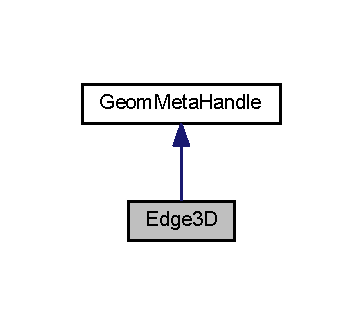
\includegraphics[width=174pt]{class_edge3_d__inherit__graph}
\end{center}
\end{figure}


Collaboration diagram for Edge3\-D\-:\nopagebreak
\begin{figure}[H]
\begin{center}
\leavevmode
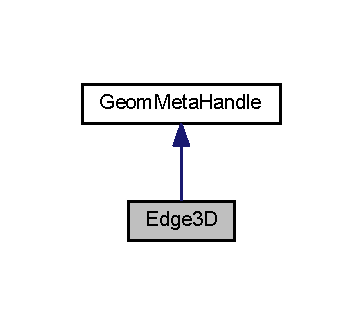
\includegraphics[width=174pt]{class_edge3_d__coll__graph}
\end{center}
\end{figure}
\subsection*{Public Member Functions}
\begin{DoxyCompactItemize}
\item 
\hypertarget{class_edge3_d_a6f25535dfee47bf06832243b11207ba6}{\hyperlink{class_edge3_d_a6f25535dfee47bf06832243b11207ba6}{Edge3\-D} ()}\label{class_edge3_d_a6f25535dfee47bf06832243b11207ba6}

\begin{DoxyCompactList}\small\item\em Constructor. Member variables are set to zero values. \end{DoxyCompactList}\item 
\hyperlink{class_edge3_d_a2c4d543fd8a4ffe272539547800c712c}{Edge3\-D} (const \hyperlink{vertex_8h_a72202e57358ed73cd212e9a2eaf39aeb}{G\-E\-O\-M\-H\-A\-N\-D\-L\-E} start, const \hyperlink{vertex_8h_a72202e57358ed73cd212e9a2eaf39aeb}{G\-E\-O\-M\-H\-A\-N\-D\-L\-E} end, const Q\-Vector3\-D midpoint)
\begin{DoxyCompactList}\small\item\em Constructor specifying start and end vertices and the midpoint of the edge. \end{DoxyCompactList}\item 
\hyperlink{class_edge3_d_af04a433a585de58702f3586d8a52219d}{Edge3\-D} (const \hyperlink{vertex_8h_a72202e57358ed73cd212e9a2eaf39aeb}{G\-E\-O\-M\-H\-A\-N\-D\-L\-E} start, const \hyperlink{vertex_8h_a72202e57358ed73cd212e9a2eaf39aeb}{G\-E\-O\-M\-H\-A\-N\-D\-L\-E} end, const \hyperlink{vertex_8h_a72202e57358ed73cd212e9a2eaf39aeb}{G\-E\-O\-M\-H\-A\-N\-D\-L\-E} rightface, const \hyperlink{vertex_8h_a72202e57358ed73cd212e9a2eaf39aeb}{G\-E\-O\-M\-H\-A\-N\-D\-L\-E} leftface, const Q\-Vector3\-D midpoint)
\begin{DoxyCompactList}\small\item\em Constructor specifying faces as well as vertices. \end{DoxyCompactList}\item 
\hyperlink{vertex_8h_a72202e57358ed73cd212e9a2eaf39aeb}{G\-E\-O\-M\-H\-A\-N\-D\-L\-E} \hyperlink{class_edge3_d_a061cf7a8c3324e564d42283702454e69}{get\-Start\-Vertex} () const 
\begin{DoxyCompactList}\small\item\em Returns the start vertex for this edge. \end{DoxyCompactList}\item 
\hyperlink{vertex_8h_a72202e57358ed73cd212e9a2eaf39aeb}{G\-E\-O\-M\-H\-A\-N\-D\-L\-E} \hyperlink{class_edge3_d_aa845b1590748b1606697afafb9b33c73}{get\-End\-Vertex} () const 
\begin{DoxyCompactList}\small\item\em Returns the end vertex of this edge. \end{DoxyCompactList}\item 
\hyperlink{vertex_8h_a72202e57358ed73cd212e9a2eaf39aeb}{G\-E\-O\-M\-H\-A\-N\-D\-L\-E} \hyperlink{class_edge3_d_a7dd9278b01fed4abf702c17eeb5c7d8b}{get\-Right\-Face} () const 
\begin{DoxyCompactList}\small\item\em Returns the edge's right face. \end{DoxyCompactList}\item 
\hyperlink{vertex_8h_a72202e57358ed73cd212e9a2eaf39aeb}{G\-E\-O\-M\-H\-A\-N\-D\-L\-E} \hyperlink{class_edge3_d_aaa398af751fda9e8b2192efef0810dc0}{get\-Left\-Face} () const 
\begin{DoxyCompactList}\small\item\em Returns the edge's left face. \end{DoxyCompactList}\item 
Q\-Vector3\-D \hyperlink{class_edge3_d_a2b97448e7bb66cf25e4bcdcff315ab5e}{get\-Midpoint} () const 
\begin{DoxyCompactList}\small\item\em Returns the edge's midpoint. \end{DoxyCompactList}\item 
\hyperlink{vertex_8h_a72202e57358ed73cd212e9a2eaf39aeb}{G\-E\-O\-M\-H\-A\-N\-D\-L\-E} \hyperlink{class_edge3_d_a34d681aaa672935753f2619ebace572b}{get\-Parent\-Solid} () const 
\begin{DoxyCompactList}\small\item\em Returns the handle of the parent solid of this edge. \end{DoxyCompactList}\item 
\hyperlink{vertex_8h_a72202e57358ed73cd212e9a2eaf39aeb}{G\-E\-O\-M\-H\-A\-N\-D\-L\-E} \hyperlink{class_edge3_d_a890650509dd10950ebaa358a349df4c7}{get\-Handle} () const 
\begin{DoxyCompactList}\small\item\em Returns this edge's geometry handle. \end{DoxyCompactList}\item 
void \hyperlink{class_edge3_d_a0533442646913ae69832e3178fa72f9a}{set\-Start\-Vertex} (const \hyperlink{vertex_8h_a72202e57358ed73cd212e9a2eaf39aeb}{G\-E\-O\-M\-H\-A\-N\-D\-L\-E} v)
\begin{DoxyCompactList}\small\item\em Sets the edge's start vertex. \end{DoxyCompactList}\item 
void \hyperlink{class_edge3_d_a32ff76ad3559822c44c8faa8519fdf74}{set\-End\-Vertex} (const \hyperlink{vertex_8h_a72202e57358ed73cd212e9a2eaf39aeb}{G\-E\-O\-M\-H\-A\-N\-D\-L\-E} v)
\begin{DoxyCompactList}\small\item\em Sets the edge's end vertex. \end{DoxyCompactList}\item 
void \hyperlink{class_edge3_d_a9960f64e5fceb5a6dc828893fe704cb6}{set\-Right\-Face} (const \hyperlink{vertex_8h_a72202e57358ed73cd212e9a2eaf39aeb}{G\-E\-O\-M\-H\-A\-N\-D\-L\-E} f)
\begin{DoxyCompactList}\small\item\em Sets the edge's right face. \end{DoxyCompactList}\item 
void \hyperlink{class_edge3_d_a1d87d3eed968ddce326ac07cc7c98e34}{set\-Left\-Face} (const \hyperlink{vertex_8h_a72202e57358ed73cd212e9a2eaf39aeb}{G\-E\-O\-M\-H\-A\-N\-D\-L\-E} f)
\begin{DoxyCompactList}\small\item\em Sets the edge's left face. \end{DoxyCompactList}\item 
void \hyperlink{class_edge3_d_a5b5e77a0d19f391cf987510111bc32f6}{set\-Midpoint} (const Q\-Vector3\-D mid)
\begin{DoxyCompactList}\small\item\em Sets the edge's midpoint. \end{DoxyCompactList}\item 
void \hyperlink{class_edge3_d_ad905287b0350a41fcf82c638e247255c}{set\-Parent\-Solid} (const \hyperlink{vertex_8h_a72202e57358ed73cd212e9a2eaf39aeb}{G\-E\-O\-M\-H\-A\-N\-D\-L\-E} handle)
\begin{DoxyCompactList}\small\item\em Sets the parent solid handle for this edge. \end{DoxyCompactList}\item 
void \hyperlink{class_edge3_d_a7ad6b919f69ee151ce78a3d5d2b41096}{set\-Handle} (const \hyperlink{vertex_8h_a72202e57358ed73cd212e9a2eaf39aeb}{G\-E\-O\-M\-H\-A\-N\-D\-L\-E} handle)
\begin{DoxyCompactList}\small\item\em Sets this edge's handle. \end{DoxyCompactList}\item 
bool \hyperlink{class_edge3_d_a9cd240bf4c0f68b3085777935e11fb85}{calc\-Midpoint} (\hyperlink{class_solid3_d}{Solid3\-D} \&parent)
\begin{DoxyCompactList}\small\item\em Given a parent solid, calculates the mid-\/point of the edge by looking up the vertices it references. \end{DoxyCompactList}\end{DoxyCompactItemize}
\subsection*{Additional Inherited Members}


\subsection{Detailed Description}
An edge links two vertices and two faces, referenced by their geometry handles.\par
 When considering travelling along the edge from the beginning to end vertex, the normals of the faces either side of the edge can be considered to point clockwise or anticlockwise around the edge. The face with an anticlockwise-\/pointing normal is denoted the \char`\"{}right\char`\"{} face (if the normal were pointing upwards the face would be positioned to the right of the edge) and the face with the clockwise-\/pointing normal is denoted the \char`\"{}left\char`\"{} face. If both normals are pointing in the same direction (either clockwise or anticlockwise) it is not defined which face is denoted left and which right. 

\subsection{Constructor \& Destructor Documentation}
\hypertarget{class_edge3_d_a2c4d543fd8a4ffe272539547800c712c}{\index{Edge3\-D@{Edge3\-D}!Edge3\-D@{Edge3\-D}}
\index{Edge3\-D@{Edge3\-D}!Edge3D@{Edge3\-D}}
\subsubsection[{Edge3\-D}]{\setlength{\rightskip}{0pt plus 5cm}Edge3\-D\-::\-Edge3\-D (
\begin{DoxyParamCaption}
\item[{const {\bf G\-E\-O\-M\-H\-A\-N\-D\-L\-E}}]{start, }
\item[{const {\bf G\-E\-O\-M\-H\-A\-N\-D\-L\-E}}]{end, }
\item[{const Q\-Vector3\-D}]{midpoint}
\end{DoxyParamCaption}
)\hspace{0.3cm}{\ttfamily [inline]}}}\label{class_edge3_d_a2c4d543fd8a4ffe272539547800c712c}


Constructor specifying start and end vertices and the midpoint of the edge. 


\begin{DoxyParams}{Parameters}
{\em start} & I\-D of vertex this edge starts at. \\
\hline
{\em end} & I\-D of vertex this edge ends at. \\
\hline
{\em midpoint} & Co-\/ordinates of the edge's midpoint. \\
\hline
\end{DoxyParams}
\hypertarget{class_edge3_d_af04a433a585de58702f3586d8a52219d}{\index{Edge3\-D@{Edge3\-D}!Edge3\-D@{Edge3\-D}}
\index{Edge3\-D@{Edge3\-D}!Edge3D@{Edge3\-D}}
\subsubsection[{Edge3\-D}]{\setlength{\rightskip}{0pt plus 5cm}Edge3\-D\-::\-Edge3\-D (
\begin{DoxyParamCaption}
\item[{const {\bf G\-E\-O\-M\-H\-A\-N\-D\-L\-E}}]{start, }
\item[{const {\bf G\-E\-O\-M\-H\-A\-N\-D\-L\-E}}]{end, }
\item[{const {\bf G\-E\-O\-M\-H\-A\-N\-D\-L\-E}}]{rightface, }
\item[{const {\bf G\-E\-O\-M\-H\-A\-N\-D\-L\-E}}]{leftface, }
\item[{const Q\-Vector3\-D}]{midpoint}
\end{DoxyParamCaption}
)\hspace{0.3cm}{\ttfamily [inline]}}}\label{class_edge3_d_af04a433a585de58702f3586d8a52219d}


Constructor specifying faces as well as vertices. 


\begin{DoxyParams}{Parameters}
{\em start} & I\-D of vertex this edge starts at. \\
\hline
{\em end} & I\-D of vertex this edge ends at. \\
\hline
{\em rightface} & Face to the right of this edge (see page description). \\
\hline
{\em leftface} & Face to the left of this edge (see page description). \\
\hline
{\em midpoint} & Co-\/ordinates of the edge's midpoint. \\
\hline
\end{DoxyParams}


\subsection{Member Function Documentation}
\hypertarget{class_edge3_d_a9cd240bf4c0f68b3085777935e11fb85}{\index{Edge3\-D@{Edge3\-D}!calc\-Midpoint@{calc\-Midpoint}}
\index{calc\-Midpoint@{calc\-Midpoint}!Edge3D@{Edge3\-D}}
\subsubsection[{calc\-Midpoint}]{\setlength{\rightskip}{0pt plus 5cm}bool Edge3\-D\-::calc\-Midpoint (
\begin{DoxyParamCaption}
\item[{{\bf Solid3\-D} \&}]{parent}
\end{DoxyParamCaption}
)}}\label{class_edge3_d_a9cd240bf4c0f68b3085777935e11fb85}


Given a parent solid, calculates the mid-\/point of the edge by looking up the vertices it references. 


\begin{DoxyParams}{Parameters}
{\em parent} & Parent solid of this edge. \\
\hline
\end{DoxyParams}
\hypertarget{class_edge3_d_aa845b1590748b1606697afafb9b33c73}{\index{Edge3\-D@{Edge3\-D}!get\-End\-Vertex@{get\-End\-Vertex}}
\index{get\-End\-Vertex@{get\-End\-Vertex}!Edge3D@{Edge3\-D}}
\subsubsection[{get\-End\-Vertex}]{\setlength{\rightskip}{0pt plus 5cm}{\bf G\-E\-O\-M\-H\-A\-N\-D\-L\-E} Edge3\-D\-::get\-End\-Vertex (
\begin{DoxyParamCaption}
{}
\end{DoxyParamCaption}
) const\hspace{0.3cm}{\ttfamily [inline]}}}\label{class_edge3_d_aa845b1590748b1606697afafb9b33c73}


Returns the end vertex of this edge. 

\begin{DoxyReturn}{Returns}
End vertex I\-D. 
\end{DoxyReturn}
\hypertarget{class_edge3_d_a890650509dd10950ebaa358a349df4c7}{\index{Edge3\-D@{Edge3\-D}!get\-Handle@{get\-Handle}}
\index{get\-Handle@{get\-Handle}!Edge3D@{Edge3\-D}}
\subsubsection[{get\-Handle}]{\setlength{\rightskip}{0pt plus 5cm}{\bf G\-E\-O\-M\-H\-A\-N\-D\-L\-E} Edge3\-D\-::get\-Handle (
\begin{DoxyParamCaption}
{}
\end{DoxyParamCaption}
) const\hspace{0.3cm}{\ttfamily [inline]}}}\label{class_edge3_d_a890650509dd10950ebaa358a349df4c7}


Returns this edge's geometry handle. 

\begin{DoxyReturn}{Returns}
Handle for this edge. 
\end{DoxyReturn}
\hypertarget{class_edge3_d_aaa398af751fda9e8b2192efef0810dc0}{\index{Edge3\-D@{Edge3\-D}!get\-Left\-Face@{get\-Left\-Face}}
\index{get\-Left\-Face@{get\-Left\-Face}!Edge3D@{Edge3\-D}}
\subsubsection[{get\-Left\-Face}]{\setlength{\rightskip}{0pt plus 5cm}{\bf G\-E\-O\-M\-H\-A\-N\-D\-L\-E} Edge3\-D\-::get\-Left\-Face (
\begin{DoxyParamCaption}
{}
\end{DoxyParamCaption}
) const\hspace{0.3cm}{\ttfamily [inline]}}}\label{class_edge3_d_aaa398af751fda9e8b2192efef0810dc0}


Returns the edge's left face. 

\begin{DoxyReturn}{Returns}
Left face I\-D (see page description). 
\end{DoxyReturn}
\hypertarget{class_edge3_d_a2b97448e7bb66cf25e4bcdcff315ab5e}{\index{Edge3\-D@{Edge3\-D}!get\-Midpoint@{get\-Midpoint}}
\index{get\-Midpoint@{get\-Midpoint}!Edge3D@{Edge3\-D}}
\subsubsection[{get\-Midpoint}]{\setlength{\rightskip}{0pt plus 5cm}Q\-Vector3\-D Edge3\-D\-::get\-Midpoint (
\begin{DoxyParamCaption}
{}
\end{DoxyParamCaption}
) const\hspace{0.3cm}{\ttfamily [inline]}}}\label{class_edge3_d_a2b97448e7bb66cf25e4bcdcff315ab5e}


Returns the edge's midpoint. 

\begin{DoxyReturn}{Returns}
Co-\/ordinates of midpoint of edge. 
\end{DoxyReturn}
\hypertarget{class_edge3_d_a34d681aaa672935753f2619ebace572b}{\index{Edge3\-D@{Edge3\-D}!get\-Parent\-Solid@{get\-Parent\-Solid}}
\index{get\-Parent\-Solid@{get\-Parent\-Solid}!Edge3D@{Edge3\-D}}
\subsubsection[{get\-Parent\-Solid}]{\setlength{\rightskip}{0pt plus 5cm}{\bf G\-E\-O\-M\-H\-A\-N\-D\-L\-E} Edge3\-D\-::get\-Parent\-Solid (
\begin{DoxyParamCaption}
{}
\end{DoxyParamCaption}
) const\hspace{0.3cm}{\ttfamily [inline]}}}\label{class_edge3_d_a34d681aaa672935753f2619ebace572b}


Returns the handle of the parent solid of this edge. 

\begin{DoxyReturn}{Returns}
Parent solid handle. 
\end{DoxyReturn}
\hypertarget{class_edge3_d_a7dd9278b01fed4abf702c17eeb5c7d8b}{\index{Edge3\-D@{Edge3\-D}!get\-Right\-Face@{get\-Right\-Face}}
\index{get\-Right\-Face@{get\-Right\-Face}!Edge3D@{Edge3\-D}}
\subsubsection[{get\-Right\-Face}]{\setlength{\rightskip}{0pt plus 5cm}{\bf G\-E\-O\-M\-H\-A\-N\-D\-L\-E} Edge3\-D\-::get\-Right\-Face (
\begin{DoxyParamCaption}
{}
\end{DoxyParamCaption}
) const\hspace{0.3cm}{\ttfamily [inline]}}}\label{class_edge3_d_a7dd9278b01fed4abf702c17eeb5c7d8b}


Returns the edge's right face. 

\begin{DoxyReturn}{Returns}
Right face I\-D (see page description). 
\end{DoxyReturn}
\hypertarget{class_edge3_d_a061cf7a8c3324e564d42283702454e69}{\index{Edge3\-D@{Edge3\-D}!get\-Start\-Vertex@{get\-Start\-Vertex}}
\index{get\-Start\-Vertex@{get\-Start\-Vertex}!Edge3D@{Edge3\-D}}
\subsubsection[{get\-Start\-Vertex}]{\setlength{\rightskip}{0pt plus 5cm}{\bf G\-E\-O\-M\-H\-A\-N\-D\-L\-E} Edge3\-D\-::get\-Start\-Vertex (
\begin{DoxyParamCaption}
{}
\end{DoxyParamCaption}
) const\hspace{0.3cm}{\ttfamily [inline]}}}\label{class_edge3_d_a061cf7a8c3324e564d42283702454e69}


Returns the start vertex for this edge. 

\begin{DoxyReturn}{Returns}
Start vertex I\-D. 
\end{DoxyReturn}
\hypertarget{class_edge3_d_a32ff76ad3559822c44c8faa8519fdf74}{\index{Edge3\-D@{Edge3\-D}!set\-End\-Vertex@{set\-End\-Vertex}}
\index{set\-End\-Vertex@{set\-End\-Vertex}!Edge3D@{Edge3\-D}}
\subsubsection[{set\-End\-Vertex}]{\setlength{\rightskip}{0pt plus 5cm}void Edge3\-D\-::set\-End\-Vertex (
\begin{DoxyParamCaption}
\item[{const {\bf G\-E\-O\-M\-H\-A\-N\-D\-L\-E}}]{v}
\end{DoxyParamCaption}
)\hspace{0.3cm}{\ttfamily [inline]}}}\label{class_edge3_d_a32ff76ad3559822c44c8faa8519fdf74}


Sets the edge's end vertex. 


\begin{DoxyParams}{Parameters}
{\em v} & Vertex I\-D to set. \\
\hline
\end{DoxyParams}
\hypertarget{class_edge3_d_a7ad6b919f69ee151ce78a3d5d2b41096}{\index{Edge3\-D@{Edge3\-D}!set\-Handle@{set\-Handle}}
\index{set\-Handle@{set\-Handle}!Edge3D@{Edge3\-D}}
\subsubsection[{set\-Handle}]{\setlength{\rightskip}{0pt plus 5cm}void Edge3\-D\-::set\-Handle (
\begin{DoxyParamCaption}
\item[{const {\bf G\-E\-O\-M\-H\-A\-N\-D\-L\-E}}]{handle}
\end{DoxyParamCaption}
)\hspace{0.3cm}{\ttfamily [inline]}}}\label{class_edge3_d_a7ad6b919f69ee151ce78a3d5d2b41096}


Sets this edge's handle. 


\begin{DoxyParams}{Parameters}
{\em handle} & Handle to set. \\
\hline
\end{DoxyParams}
\hypertarget{class_edge3_d_a1d87d3eed968ddce326ac07cc7c98e34}{\index{Edge3\-D@{Edge3\-D}!set\-Left\-Face@{set\-Left\-Face}}
\index{set\-Left\-Face@{set\-Left\-Face}!Edge3D@{Edge3\-D}}
\subsubsection[{set\-Left\-Face}]{\setlength{\rightskip}{0pt plus 5cm}void Edge3\-D\-::set\-Left\-Face (
\begin{DoxyParamCaption}
\item[{const {\bf G\-E\-O\-M\-H\-A\-N\-D\-L\-E}}]{f}
\end{DoxyParamCaption}
)\hspace{0.3cm}{\ttfamily [inline]}}}\label{class_edge3_d_a1d87d3eed968ddce326ac07cc7c98e34}


Sets the edge's left face. 


\begin{DoxyParams}{Parameters}
{\em f} & Face I\-D to set. \\
\hline
\end{DoxyParams}
\hypertarget{class_edge3_d_a5b5e77a0d19f391cf987510111bc32f6}{\index{Edge3\-D@{Edge3\-D}!set\-Midpoint@{set\-Midpoint}}
\index{set\-Midpoint@{set\-Midpoint}!Edge3D@{Edge3\-D}}
\subsubsection[{set\-Midpoint}]{\setlength{\rightskip}{0pt plus 5cm}void Edge3\-D\-::set\-Midpoint (
\begin{DoxyParamCaption}
\item[{const Q\-Vector3\-D}]{mid}
\end{DoxyParamCaption}
)\hspace{0.3cm}{\ttfamily [inline]}}}\label{class_edge3_d_a5b5e77a0d19f391cf987510111bc32f6}


Sets the edge's midpoint. 


\begin{DoxyParams}{Parameters}
{\em mid} & Co-\/ordinates of midpoint. \\
\hline
\end{DoxyParams}
\hypertarget{class_edge3_d_ad905287b0350a41fcf82c638e247255c}{\index{Edge3\-D@{Edge3\-D}!set\-Parent\-Solid@{set\-Parent\-Solid}}
\index{set\-Parent\-Solid@{set\-Parent\-Solid}!Edge3D@{Edge3\-D}}
\subsubsection[{set\-Parent\-Solid}]{\setlength{\rightskip}{0pt plus 5cm}void Edge3\-D\-::set\-Parent\-Solid (
\begin{DoxyParamCaption}
\item[{const {\bf G\-E\-O\-M\-H\-A\-N\-D\-L\-E}}]{handle}
\end{DoxyParamCaption}
)\hspace{0.3cm}{\ttfamily [inline]}}}\label{class_edge3_d_ad905287b0350a41fcf82c638e247255c}


Sets the parent solid handle for this edge. 


\begin{DoxyParams}{Parameters}
{\em handle} & Handle to set. \\
\hline
\end{DoxyParams}
\hypertarget{class_edge3_d_a9960f64e5fceb5a6dc828893fe704cb6}{\index{Edge3\-D@{Edge3\-D}!set\-Right\-Face@{set\-Right\-Face}}
\index{set\-Right\-Face@{set\-Right\-Face}!Edge3D@{Edge3\-D}}
\subsubsection[{set\-Right\-Face}]{\setlength{\rightskip}{0pt plus 5cm}void Edge3\-D\-::set\-Right\-Face (
\begin{DoxyParamCaption}
\item[{const {\bf G\-E\-O\-M\-H\-A\-N\-D\-L\-E}}]{f}
\end{DoxyParamCaption}
)\hspace{0.3cm}{\ttfamily [inline]}}}\label{class_edge3_d_a9960f64e5fceb5a6dc828893fe704cb6}


Sets the edge's right face. 


\begin{DoxyParams}{Parameters}
{\em f} & Face I\-D to set. \\
\hline
\end{DoxyParams}
\hypertarget{class_edge3_d_a0533442646913ae69832e3178fa72f9a}{\index{Edge3\-D@{Edge3\-D}!set\-Start\-Vertex@{set\-Start\-Vertex}}
\index{set\-Start\-Vertex@{set\-Start\-Vertex}!Edge3D@{Edge3\-D}}
\subsubsection[{set\-Start\-Vertex}]{\setlength{\rightskip}{0pt plus 5cm}void Edge3\-D\-::set\-Start\-Vertex (
\begin{DoxyParamCaption}
\item[{const {\bf G\-E\-O\-M\-H\-A\-N\-D\-L\-E}}]{v}
\end{DoxyParamCaption}
)\hspace{0.3cm}{\ttfamily [inline]}}}\label{class_edge3_d_a0533442646913ae69832e3178fa72f9a}


Sets the edge's start vertex. 


\begin{DoxyParams}{Parameters}
{\em v} & Vertex I\-D to set. \\
\hline
\end{DoxyParams}


The documentation for this class was generated from the following files\-:\begin{DoxyCompactItemize}
\item 
app/\hyperlink{edge_8h}{edge.\-h}\item 
app/edge.\-cpp\end{DoxyCompactItemize}

\hypertarget{class_face3_d}{\section{Face3\-D Class Reference}
\label{class_face3_d}\index{Face3\-D@{Face3\-D}}
}


Class representing a 3\-D face.  




{\ttfamily \#include $<$face.\-h$>$}



Inheritance diagram for Face3\-D\-:
\nopagebreak
\begin{figure}[H]
\begin{center}
\leavevmode
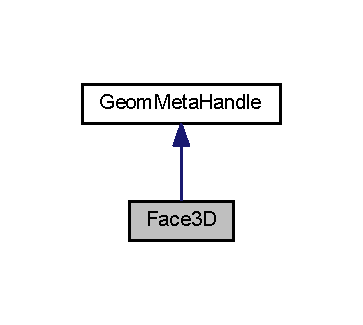
\includegraphics[width=174pt]{class_face3_d__inherit__graph}
\end{center}
\end{figure}


Collaboration diagram for Face3\-D\-:
\nopagebreak
\begin{figure}[H]
\begin{center}
\leavevmode
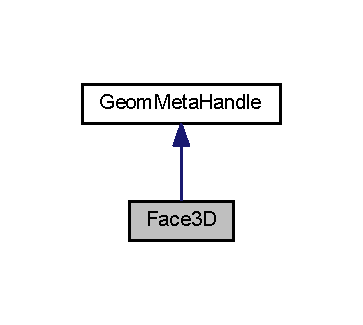
\includegraphics[width=174pt]{class_face3_d__coll__graph}
\end{center}
\end{figure}
\subsection*{Public Member Functions}
\begin{DoxyCompactItemize}
\item 
\hypertarget{class_face3_d_af64a4a5fe2a8f06dd684bff91041e0cb}{\hyperlink{class_face3_d_af64a4a5fe2a8f06dd684bff91041e0cb}{Face3\-D} ()}\label{class_face3_d_af64a4a5fe2a8f06dd684bff91041e0cb}

\begin{DoxyCompactList}\small\item\em Constructor. Sets member variables to default values. \end{DoxyCompactList}\item 
\hyperlink{class_face3_d_a6113068475ee9edc57445f8eac3d4f5b}{Face3\-D} (const \hyperlink{class_plane}{Plane} p, const Q\-Vector3\-D centre=\hyperlink{matlib_8h_ac2de4dab97258eff87e0a1253a2d1a29}{V\-E\-C3\-\_\-\-O\-R\-I\-G\-I\-N})
\begin{DoxyCompactList}\small\item\em Constructor specifying plane and centre point of face. \end{DoxyCompactList}\item 
\hypertarget{class_face3_d_af7dc0f5eb3359689d7617cad7fe65797}{\hyperlink{class_face3_d_af7dc0f5eb3359689d7617cad7fe65797}{$\sim$\-Face3\-D} ()}\label{class_face3_d_af7dc0f5eb3359689d7617cad7fe65797}

\begin{DoxyCompactList}\small\item\em Destructor. \end{DoxyCompactList}\item 
int \hyperlink{class_face3_d_a83db8beee23e03ff24cd9b0649e8269c}{get\-Edge\-Count} () const 
\begin{DoxyCompactList}\small\item\em Returns the number of edges this face contains. \end{DoxyCompactList}\item 
\hyperlink{vertex_8h_a72202e57358ed73cd212e9a2eaf39aeb}{G\-E\-O\-M\-H\-A\-N\-D\-L\-E} \hyperlink{class_face3_d_a7a44b794e450e4e9784484876e10710b}{get\-Edge\-Handle} (const int index) const 
\begin{DoxyCompactList}\small\item\em Returns the handle to the edge at a specific index in the edge list. Index must be within range. \end{DoxyCompactList}\item 
\hyperlink{class_plane}{Plane} \hyperlink{class_face3_d_a1e3d068cffc33876100a3affc496e8eb}{get\-Plane} () const 
\begin{DoxyCompactList}\small\item\em Gets the plane that represents this face's surface. \end{DoxyCompactList}\item 
Q\-Vector3\-D \hyperlink{class_face3_d_a0dfbcd5b1fa9fd18d2b09064d5dff8ac}{get\-Normal} () const 
\begin{DoxyCompactList}\small\item\em Gets this face's normal. \end{DoxyCompactList}\item 
bool \hyperlink{class_face3_d_a9e8a8bcd2337cc8aeaa231aba7c5996b}{is\-Plane\-Valid} () const 
\begin{DoxyCompactList}\small\item\em Returns whether the face's plane is valid. \end{DoxyCompactList}\item 
Q\-Vector3\-D \hyperlink{class_face3_d_a34bc3d8aeb903d18d3f05b6af299fdff}{get\-Centre\-Point} () const 
\begin{DoxyCompactList}\small\item\em Gets the central point of the face. \end{DoxyCompactList}\item 
\hyperlink{vertex_8h_a72202e57358ed73cd212e9a2eaf39aeb}{G\-E\-O\-M\-H\-A\-N\-D\-L\-E} \hyperlink{class_face3_d_a84bf13a7355baeeedf35b6da66c064ec}{get\-Parent\-Solid} () const 
\begin{DoxyCompactList}\small\item\em Gets the hand of the parent solid of this face. \end{DoxyCompactList}\item 
\hyperlink{vertex_8h_a72202e57358ed73cd212e9a2eaf39aeb}{G\-E\-O\-M\-H\-A\-N\-D\-L\-E} \hyperlink{class_face3_d_ad0bc376833756ff964ad8967fc459c8f}{get\-Handle} () const 
\begin{DoxyCompactList}\small\item\em Gets this face's handle. \end{DoxyCompactList}\item 
bool \hyperlink{class_face3_d_a7b6289ce08b7e07e050641449d42a4d7}{contains\-Edge} (const \hyperlink{vertex_8h_a72202e57358ed73cd212e9a2eaf39aeb}{G\-E\-O\-M\-H\-A\-N\-D\-L\-E} edge) const 
\begin{DoxyCompactList}\small\item\em Returns whether this face contains an edge with the specified handle. \end{DoxyCompactList}\item 
bool \hyperlink{class_face3_d_ae8daf489ffc7b411edb78b2e62e95e80}{contains\-Any\-Edge} (const Q\-List$<$ \hyperlink{vertex_8h_a72202e57358ed73cd212e9a2eaf39aeb}{G\-E\-O\-M\-H\-A\-N\-D\-L\-E} $>$ \&edges) const 
\begin{DoxyCompactList}\small\item\em Returns whether this face contains any of the edges in the list provided. \end{DoxyCompactList}\item 
void \hyperlink{class_face3_d_ab58095c8043c2f08751327a6399365c9}{set\-Plane} (const \hyperlink{class_plane}{Plane} p)
\begin{DoxyCompactList}\small\item\em Set's the face's plane. \end{DoxyCompactList}\item 
void \hyperlink{class_face3_d_aedb4458bdb3b06dddd830c53726aa844}{set\-Centre\-Point} (const Q\-Vector3\-D centre)
\begin{DoxyCompactList}\small\item\em Sets the face's central point. \end{DoxyCompactList}\item 
void \hyperlink{class_face3_d_aaf0b823d7e83800962181136a3806be5}{set\-Parent\-Solid} (const \hyperlink{vertex_8h_a72202e57358ed73cd212e9a2eaf39aeb}{G\-E\-O\-M\-H\-A\-N\-D\-L\-E} handle)
\begin{DoxyCompactList}\small\item\em Sets the parent solid handle for this face. \end{DoxyCompactList}\item 
void \hyperlink{class_face3_d_a3f040832e7d61cddc9286acce1597bfd}{set\-Handle} (const \hyperlink{vertex_8h_a72202e57358ed73cd212e9a2eaf39aeb}{G\-E\-O\-M\-H\-A\-N\-D\-L\-E} handle)
\begin{DoxyCompactList}\small\item\em Sets the handle of this face. \end{DoxyCompactList}\item 
void \hyperlink{class_face3_d_a67c54bddb563a26bdde53b59ba38ae86}{add\-Edge} (\hyperlink{vertex_8h_a72202e57358ed73cd212e9a2eaf39aeb}{G\-E\-O\-M\-H\-A\-N\-D\-L\-E} edge)
\begin{DoxyCompactList}\small\item\em Adds an edge to this face. The edge must already exist in the face's parent solid. \end{DoxyCompactList}\item 
bool \hyperlink{class_face3_d_a5f360979f999dfaa2f7be7ed3c66ef0f}{is\-Composite} ()
\begin{DoxyCompactList}\small\item\em Returns whether the face is composite. Composite faces contain more than just three edges (ie. they are composed of more than one triangle). \end{DoxyCompactList}\end{DoxyCompactItemize}
\subsection*{Additional Inherited Members}


\subsection{Detailed Description}
Class representing a 3\-D face. 

Solids are made up of faces, which are built up from lists of member edges. Faces also contain plane information (for easy conversion to/from V\-M\-Fs). The direction of the face's edges according to their start/end vertices does not necessarily have to be clockwise (this would be impractical) but the edges do have to form a closed, contiguous loop from the beginning to the end of the list, the last vertex of the last edge being the first vertex of the first edge. The loop should form a convex 2\-D polygon. 

\subsection{Constructor \& Destructor Documentation}
\hypertarget{class_face3_d_a6113068475ee9edc57445f8eac3d4f5b}{\index{Face3\-D@{Face3\-D}!Face3\-D@{Face3\-D}}
\index{Face3\-D@{Face3\-D}!Face3D@{Face3\-D}}
\subsubsection[{Face3\-D}]{\setlength{\rightskip}{0pt plus 5cm}Face3\-D\-::\-Face3\-D (
\begin{DoxyParamCaption}
\item[{const {\bf Plane}}]{p, }
\item[{const Q\-Vector3\-D}]{centre = {\ttfamily {\bf V\-E\-C3\-\_\-\-O\-R\-I\-G\-I\-N}}}
\end{DoxyParamCaption}
)\hspace{0.3cm}{\ttfamily [inline]}}}\label{class_face3_d_a6113068475ee9edc57445f8eac3d4f5b}


Constructor specifying plane and centre point of face. 


\begin{DoxyParams}{Parameters}
{\em p} & \\
\hline
{\em centre} & \\
\hline
\end{DoxyParams}


\subsection{Member Function Documentation}
\hypertarget{class_face3_d_a67c54bddb563a26bdde53b59ba38ae86}{\index{Face3\-D@{Face3\-D}!add\-Edge@{add\-Edge}}
\index{add\-Edge@{add\-Edge}!Face3D@{Face3\-D}}
\subsubsection[{add\-Edge}]{\setlength{\rightskip}{0pt plus 5cm}void Face3\-D\-::add\-Edge (
\begin{DoxyParamCaption}
\item[{{\bf G\-E\-O\-M\-H\-A\-N\-D\-L\-E}}]{edge}
\end{DoxyParamCaption}
)\hspace{0.3cm}{\ttfamily [inline]}}}\label{class_face3_d_a67c54bddb563a26bdde53b59ba38ae86}


Adds an edge to this face. The edge must already exist in the face's parent solid. 

\begin{DoxyNote}{Note}
Does N\-O\-T check whether the edge already exists in the face. 
\end{DoxyNote}

\begin{DoxyParams}{Parameters}
{\em edge} & Handle of the edge to add. \\
\hline
\end{DoxyParams}
\hypertarget{class_face3_d_ae8daf489ffc7b411edb78b2e62e95e80}{\index{Face3\-D@{Face3\-D}!contains\-Any\-Edge@{contains\-Any\-Edge}}
\index{contains\-Any\-Edge@{contains\-Any\-Edge}!Face3D@{Face3\-D}}
\subsubsection[{contains\-Any\-Edge}]{\setlength{\rightskip}{0pt plus 5cm}bool Face3\-D\-::contains\-Any\-Edge (
\begin{DoxyParamCaption}
\item[{const Q\-List$<$ {\bf G\-E\-O\-M\-H\-A\-N\-D\-L\-E} $>$ \&}]{edges}
\end{DoxyParamCaption}
) const}}\label{class_face3_d_ae8daf489ffc7b411edb78b2e62e95e80}


Returns whether this face contains any of the edges in the list provided. 


\begin{DoxyParams}{Parameters}
{\em edges} & List of edge handles to check. \\
\hline
\end{DoxyParams}
\begin{DoxyReturn}{Returns}
True if the face contains any edge, false if the face contains none of the edges. 
\end{DoxyReturn}
\hypertarget{class_face3_d_a7b6289ce08b7e07e050641449d42a4d7}{\index{Face3\-D@{Face3\-D}!contains\-Edge@{contains\-Edge}}
\index{contains\-Edge@{contains\-Edge}!Face3D@{Face3\-D}}
\subsubsection[{contains\-Edge}]{\setlength{\rightskip}{0pt plus 5cm}bool Face3\-D\-::contains\-Edge (
\begin{DoxyParamCaption}
\item[{const {\bf G\-E\-O\-M\-H\-A\-N\-D\-L\-E}}]{edge}
\end{DoxyParamCaption}
) const}}\label{class_face3_d_a7b6289ce08b7e07e050641449d42a4d7}


Returns whether this face contains an edge with the specified handle. 


\begin{DoxyParams}{Parameters}
{\em edge} & Handle to check. \\
\hline
\end{DoxyParams}
\begin{DoxyReturn}{Returns}
True if the edge is contained within the face, false if not. 
\end{DoxyReturn}
\hypertarget{class_face3_d_a34bc3d8aeb903d18d3f05b6af299fdff}{\index{Face3\-D@{Face3\-D}!get\-Centre\-Point@{get\-Centre\-Point}}
\index{get\-Centre\-Point@{get\-Centre\-Point}!Face3D@{Face3\-D}}
\subsubsection[{get\-Centre\-Point}]{\setlength{\rightskip}{0pt plus 5cm}Q\-Vector3\-D Face3\-D\-::get\-Centre\-Point (
\begin{DoxyParamCaption}
{}
\end{DoxyParamCaption}
) const\hspace{0.3cm}{\ttfamily [inline]}}}\label{class_face3_d_a34bc3d8aeb903d18d3f05b6af299fdff}


Gets the central point of the face. 

\begin{DoxyReturn}{Returns}
Face centre point. 
\end{DoxyReturn}
\hypertarget{class_face3_d_a83db8beee23e03ff24cd9b0649e8269c}{\index{Face3\-D@{Face3\-D}!get\-Edge\-Count@{get\-Edge\-Count}}
\index{get\-Edge\-Count@{get\-Edge\-Count}!Face3D@{Face3\-D}}
\subsubsection[{get\-Edge\-Count}]{\setlength{\rightskip}{0pt plus 5cm}int Face3\-D\-::get\-Edge\-Count (
\begin{DoxyParamCaption}
{}
\end{DoxyParamCaption}
) const\hspace{0.3cm}{\ttfamily [inline]}}}\label{class_face3_d_a83db8beee23e03ff24cd9b0649e8269c}


Returns the number of edges this face contains. 

\begin{DoxyReturn}{Returns}
Number of edges. 
\end{DoxyReturn}
\hypertarget{class_face3_d_a7a44b794e450e4e9784484876e10710b}{\index{Face3\-D@{Face3\-D}!get\-Edge\-Handle@{get\-Edge\-Handle}}
\index{get\-Edge\-Handle@{get\-Edge\-Handle}!Face3D@{Face3\-D}}
\subsubsection[{get\-Edge\-Handle}]{\setlength{\rightskip}{0pt plus 5cm}{\bf G\-E\-O\-M\-H\-A\-N\-D\-L\-E} Face3\-D\-::get\-Edge\-Handle (
\begin{DoxyParamCaption}
\item[{const int}]{index}
\end{DoxyParamCaption}
) const\hspace{0.3cm}{\ttfamily [inline]}}}\label{class_face3_d_a7a44b794e450e4e9784484876e10710b}


Returns the handle to the edge at a specific index in the edge list. Index must be within range. 


\begin{DoxyParams}{Parameters}
{\em index} & Index of edge to retrieve. \\
\hline
\end{DoxyParams}
\begin{DoxyReturn}{Returns}
Edge at this index. 
\end{DoxyReturn}
\hypertarget{class_face3_d_ad0bc376833756ff964ad8967fc459c8f}{\index{Face3\-D@{Face3\-D}!get\-Handle@{get\-Handle}}
\index{get\-Handle@{get\-Handle}!Face3D@{Face3\-D}}
\subsubsection[{get\-Handle}]{\setlength{\rightskip}{0pt plus 5cm}{\bf G\-E\-O\-M\-H\-A\-N\-D\-L\-E} Face3\-D\-::get\-Handle (
\begin{DoxyParamCaption}
{}
\end{DoxyParamCaption}
) const\hspace{0.3cm}{\ttfamily [inline]}}}\label{class_face3_d_ad0bc376833756ff964ad8967fc459c8f}


Gets this face's handle. 

\begin{DoxyReturn}{Returns}
Handle of the face. 
\end{DoxyReturn}
\hypertarget{class_face3_d_a0dfbcd5b1fa9fd18d2b09064d5dff8ac}{\index{Face3\-D@{Face3\-D}!get\-Normal@{get\-Normal}}
\index{get\-Normal@{get\-Normal}!Face3D@{Face3\-D}}
\subsubsection[{get\-Normal}]{\setlength{\rightskip}{0pt plus 5cm}Q\-Vector3\-D Face3\-D\-::get\-Normal (
\begin{DoxyParamCaption}
{}
\end{DoxyParamCaption}
) const\hspace{0.3cm}{\ttfamily [inline]}}}\label{class_face3_d_a0dfbcd5b1fa9fd18d2b09064d5dff8ac}


Gets this face's normal. 

\begin{DoxyReturn}{Returns}
Normal of face. 
\end{DoxyReturn}
\hypertarget{class_face3_d_a84bf13a7355baeeedf35b6da66c064ec}{\index{Face3\-D@{Face3\-D}!get\-Parent\-Solid@{get\-Parent\-Solid}}
\index{get\-Parent\-Solid@{get\-Parent\-Solid}!Face3D@{Face3\-D}}
\subsubsection[{get\-Parent\-Solid}]{\setlength{\rightskip}{0pt plus 5cm}{\bf G\-E\-O\-M\-H\-A\-N\-D\-L\-E} Face3\-D\-::get\-Parent\-Solid (
\begin{DoxyParamCaption}
{}
\end{DoxyParamCaption}
) const\hspace{0.3cm}{\ttfamily [inline]}}}\label{class_face3_d_a84bf13a7355baeeedf35b6da66c064ec}


Gets the hand of the parent solid of this face. 

\begin{DoxyReturn}{Returns}
Parent solid handle. 
\end{DoxyReturn}
\hypertarget{class_face3_d_a1e3d068cffc33876100a3affc496e8eb}{\index{Face3\-D@{Face3\-D}!get\-Plane@{get\-Plane}}
\index{get\-Plane@{get\-Plane}!Face3D@{Face3\-D}}
\subsubsection[{get\-Plane}]{\setlength{\rightskip}{0pt plus 5cm}{\bf Plane} Face3\-D\-::get\-Plane (
\begin{DoxyParamCaption}
{}
\end{DoxyParamCaption}
) const\hspace{0.3cm}{\ttfamily [inline]}}}\label{class_face3_d_a1e3d068cffc33876100a3affc496e8eb}


Gets the plane that represents this face's surface. 

\begin{DoxyReturn}{Returns}
\hyperlink{class_plane}{Plane} of face. 
\end{DoxyReturn}
\hypertarget{class_face3_d_a5f360979f999dfaa2f7be7ed3c66ef0f}{\index{Face3\-D@{Face3\-D}!is\-Composite@{is\-Composite}}
\index{is\-Composite@{is\-Composite}!Face3D@{Face3\-D}}
\subsubsection[{is\-Composite}]{\setlength{\rightskip}{0pt plus 5cm}bool Face3\-D\-::is\-Composite (
\begin{DoxyParamCaption}
{}
\end{DoxyParamCaption}
)\hspace{0.3cm}{\ttfamily [inline]}}}\label{class_face3_d_a5f360979f999dfaa2f7be7ed3c66ef0f}


Returns whether the face is composite. Composite faces contain more than just three edges (ie. they are composed of more than one triangle). 

\begin{DoxyReturn}{Returns}
True if face is composite, false otherwise. 
\end{DoxyReturn}
\hypertarget{class_face3_d_a9e8a8bcd2337cc8aeaa231aba7c5996b}{\index{Face3\-D@{Face3\-D}!is\-Plane\-Valid@{is\-Plane\-Valid}}
\index{is\-Plane\-Valid@{is\-Plane\-Valid}!Face3D@{Face3\-D}}
\subsubsection[{is\-Plane\-Valid}]{\setlength{\rightskip}{0pt plus 5cm}bool Face3\-D\-::is\-Plane\-Valid (
\begin{DoxyParamCaption}
{}
\end{DoxyParamCaption}
) const\hspace{0.3cm}{\ttfamily [inline]}}}\label{class_face3_d_a9e8a8bcd2337cc8aeaa231aba7c5996b}


Returns whether the face's plane is valid. 

\begin{DoxyReturn}{Returns}
True if plane is valid, false otherwise. 
\end{DoxyReturn}
\hypertarget{class_face3_d_aedb4458bdb3b06dddd830c53726aa844}{\index{Face3\-D@{Face3\-D}!set\-Centre\-Point@{set\-Centre\-Point}}
\index{set\-Centre\-Point@{set\-Centre\-Point}!Face3D@{Face3\-D}}
\subsubsection[{set\-Centre\-Point}]{\setlength{\rightskip}{0pt plus 5cm}void Face3\-D\-::set\-Centre\-Point (
\begin{DoxyParamCaption}
\item[{const Q\-Vector3\-D}]{centre}
\end{DoxyParamCaption}
)\hspace{0.3cm}{\ttfamily [inline]}}}\label{class_face3_d_aedb4458bdb3b06dddd830c53726aa844}


Sets the face's central point. 


\begin{DoxyParams}{Parameters}
{\em centre} & Centre point to set. \\
\hline
\end{DoxyParams}
\hypertarget{class_face3_d_a3f040832e7d61cddc9286acce1597bfd}{\index{Face3\-D@{Face3\-D}!set\-Handle@{set\-Handle}}
\index{set\-Handle@{set\-Handle}!Face3D@{Face3\-D}}
\subsubsection[{set\-Handle}]{\setlength{\rightskip}{0pt plus 5cm}void Face3\-D\-::set\-Handle (
\begin{DoxyParamCaption}
\item[{const {\bf G\-E\-O\-M\-H\-A\-N\-D\-L\-E}}]{handle}
\end{DoxyParamCaption}
)\hspace{0.3cm}{\ttfamily [inline]}}}\label{class_face3_d_a3f040832e7d61cddc9286acce1597bfd}


Sets the handle of this face. 


\begin{DoxyParams}{Parameters}
{\em handle} & Handle to set. \\
\hline
\end{DoxyParams}
\hypertarget{class_face3_d_aaf0b823d7e83800962181136a3806be5}{\index{Face3\-D@{Face3\-D}!set\-Parent\-Solid@{set\-Parent\-Solid}}
\index{set\-Parent\-Solid@{set\-Parent\-Solid}!Face3D@{Face3\-D}}
\subsubsection[{set\-Parent\-Solid}]{\setlength{\rightskip}{0pt plus 5cm}void Face3\-D\-::set\-Parent\-Solid (
\begin{DoxyParamCaption}
\item[{const {\bf G\-E\-O\-M\-H\-A\-N\-D\-L\-E}}]{handle}
\end{DoxyParamCaption}
)\hspace{0.3cm}{\ttfamily [inline]}}}\label{class_face3_d_aaf0b823d7e83800962181136a3806be5}


Sets the parent solid handle for this face. 


\begin{DoxyParams}{Parameters}
{\em handle} & Handle to set. \\
\hline
\end{DoxyParams}
\hypertarget{class_face3_d_ab58095c8043c2f08751327a6399365c9}{\index{Face3\-D@{Face3\-D}!set\-Plane@{set\-Plane}}
\index{set\-Plane@{set\-Plane}!Face3D@{Face3\-D}}
\subsubsection[{set\-Plane}]{\setlength{\rightskip}{0pt plus 5cm}void Face3\-D\-::set\-Plane (
\begin{DoxyParamCaption}
\item[{const {\bf Plane}}]{p}
\end{DoxyParamCaption}
)\hspace{0.3cm}{\ttfamily [inline]}}}\label{class_face3_d_ab58095c8043c2f08751327a6399365c9}


Set's the face's plane. 


\begin{DoxyParams}{Parameters}
{\em p} & \hyperlink{class_plane}{Plane} to set. \\
\hline
\end{DoxyParams}


The documentation for this class was generated from the following files\-:\begin{DoxyCompactItemize}
\item 
app/\hyperlink{face_8h}{face.\-h}\item 
app/face.\-cpp\end{DoxyCompactItemize}

\hypertarget{struct_geom_info}{\section{Geom\-Info Struct Reference}
\label{struct_geom_info}\index{Geom\-Info@{Geom\-Info}}
}


Struct to hold and pass information about geometry objects.  




{\ttfamily \#include $<$solid.\-h$>$}

\subsection*{Public Types}
\begin{DoxyCompactItemize}
\item 
enum \hyperlink{struct_geom_info_a5599514c547c57d65f341d62b65caad0}{Geom\-Type} \{ \\*
\hyperlink{struct_geom_info_a5599514c547c57d65f341d62b65caad0ac4a683020056249df8d5ec2c435ed23e}{Null} = 0, 
\hyperlink{struct_geom_info_a5599514c547c57d65f341d62b65caad0a8b3ba3bda90e2e26cfd607d3bf2f10d7}{Vertex}, 
\hyperlink{struct_geom_info_a5599514c547c57d65f341d62b65caad0af10d43145fadd1fe008918de2d5eea55}{Edge}, 
\hyperlink{struct_geom_info_a5599514c547c57d65f341d62b65caad0ade4416774f0a723c80be9ce4f02b7b60}{Face}, 
\\*
\hyperlink{struct_geom_info_a5599514c547c57d65f341d62b65caad0abf8e24db95b4ab93e5a4fb3a93919435}{Solid}
 \}
\begin{DoxyCompactList}\small\item\em Specifies what type of geometry we are describing. \end{DoxyCompactList}\end{DoxyCompactItemize}
\subsection*{Public Attributes}
\begin{DoxyCompactItemize}
\item 
\hyperlink{vertex_8h_a72202e57358ed73cd212e9a2eaf39aeb}{G\-E\-O\-M\-H\-A\-N\-D\-L\-E} \hyperlink{struct_geom_info_a38fdd8d03050ce8b279b313eb53a7862}{m\-\_\-h\-Handle}
\item 
\hyperlink{struct_geom_info_a5599514c547c57d65f341d62b65caad0}{Geom\-Type} \hyperlink{struct_geom_info_a39b0270c2fa75ee91a7b43349440974d}{m\-\_\-i\-Type}
\item 
\hyperlink{vertex_8h_a72202e57358ed73cd212e9a2eaf39aeb}{G\-E\-O\-M\-H\-A\-N\-D\-L\-E} \hyperlink{struct_geom_info_aa929dea8b11f72ae4489e73ef8f60f7a}{m\-\_\-h\-Parent\-Solid}
\end{DoxyCompactItemize}


\subsection{Detailed Description}
Struct to hold and pass information about geometry objects. 

\subsection{Member Enumeration Documentation}
\hypertarget{struct_geom_info_a5599514c547c57d65f341d62b65caad0}{\index{Geom\-Info@{Geom\-Info}!Geom\-Type@{Geom\-Type}}
\index{Geom\-Type@{Geom\-Type}!GeomInfo@{Geom\-Info}}
\subsubsection[{Geom\-Type}]{\setlength{\rightskip}{0pt plus 5cm}enum {\bf Geom\-Info\-::\-Geom\-Type}}}\label{struct_geom_info_a5599514c547c57d65f341d62b65caad0}


Specifies what type of geometry we are describing. 

\begin{Desc}
\item[Enumerator]\par
\begin{description}
\index{Null@{Null}!Geom\-Info@{Geom\-Info}}\index{Geom\-Info@{Geom\-Info}!Null@{Null}}\item[{\em 
\hypertarget{struct_geom_info_a5599514c547c57d65f341d62b65caad0ac4a683020056249df8d5ec2c435ed23e}{Null}\label{struct_geom_info_a5599514c547c57d65f341d62b65caad0ac4a683020056249df8d5ec2c435ed23e}
}]N\-U\-L\-L (invalid) \index{Vertex@{Vertex}!Geom\-Info@{Geom\-Info}}\index{Geom\-Info@{Geom\-Info}!Vertex@{Vertex}}\item[{\em 
\hypertarget{struct_geom_info_a5599514c547c57d65f341d62b65caad0a8b3ba3bda90e2e26cfd607d3bf2f10d7}{Vertex}\label{struct_geom_info_a5599514c547c57d65f341d62b65caad0a8b3ba3bda90e2e26cfd607d3bf2f10d7}
}]Vertex \index{Edge@{Edge}!Geom\-Info@{Geom\-Info}}\index{Geom\-Info@{Geom\-Info}!Edge@{Edge}}\item[{\em 
\hypertarget{struct_geom_info_a5599514c547c57d65f341d62b65caad0af10d43145fadd1fe008918de2d5eea55}{Edge}\label{struct_geom_info_a5599514c547c57d65f341d62b65caad0af10d43145fadd1fe008918de2d5eea55}
}]Edge \index{Face@{Face}!Geom\-Info@{Geom\-Info}}\index{Geom\-Info@{Geom\-Info}!Face@{Face}}\item[{\em 
\hypertarget{struct_geom_info_a5599514c547c57d65f341d62b65caad0ade4416774f0a723c80be9ce4f02b7b60}{Face}\label{struct_geom_info_a5599514c547c57d65f341d62b65caad0ade4416774f0a723c80be9ce4f02b7b60}
}]Face \index{Solid@{Solid}!Geom\-Info@{Geom\-Info}}\index{Geom\-Info@{Geom\-Info}!Solid@{Solid}}\item[{\em 
\hypertarget{struct_geom_info_a5599514c547c57d65f341d62b65caad0abf8e24db95b4ab93e5a4fb3a93919435}{Solid}\label{struct_geom_info_a5599514c547c57d65f341d62b65caad0abf8e24db95b4ab93e5a4fb3a93919435}
}]Solid \end{description}
\end{Desc}


\subsection{Member Data Documentation}
\hypertarget{struct_geom_info_a38fdd8d03050ce8b279b313eb53a7862}{\index{Geom\-Info@{Geom\-Info}!m\-\_\-h\-Handle@{m\-\_\-h\-Handle}}
\index{m\-\_\-h\-Handle@{m\-\_\-h\-Handle}!GeomInfo@{Geom\-Info}}
\subsubsection[{m\-\_\-h\-Handle}]{\setlength{\rightskip}{0pt plus 5cm}{\bf G\-E\-O\-M\-H\-A\-N\-D\-L\-E} Geom\-Info\-::m\-\_\-h\-Handle}}\label{struct_geom_info_a38fdd8d03050ce8b279b313eb53a7862}
Local handle for this object. \hypertarget{struct_geom_info_aa929dea8b11f72ae4489e73ef8f60f7a}{\index{Geom\-Info@{Geom\-Info}!m\-\_\-h\-Parent\-Solid@{m\-\_\-h\-Parent\-Solid}}
\index{m\-\_\-h\-Parent\-Solid@{m\-\_\-h\-Parent\-Solid}!GeomInfo@{Geom\-Info}}
\subsubsection[{m\-\_\-h\-Parent\-Solid}]{\setlength{\rightskip}{0pt plus 5cm}{\bf G\-E\-O\-M\-H\-A\-N\-D\-L\-E} Geom\-Info\-::m\-\_\-h\-Parent\-Solid}}\label{struct_geom_info_aa929dea8b11f72ae4489e73ef8f60f7a}
Handle to parent solid. N\-U\-L\-L if m\-\_\-i\-Type is Geom\-Type\-::\-Solid. \hypertarget{struct_geom_info_a39b0270c2fa75ee91a7b43349440974d}{\index{Geom\-Info@{Geom\-Info}!m\-\_\-i\-Type@{m\-\_\-i\-Type}}
\index{m\-\_\-i\-Type@{m\-\_\-i\-Type}!GeomInfo@{Geom\-Info}}
\subsubsection[{m\-\_\-i\-Type}]{\setlength{\rightskip}{0pt plus 5cm}{\bf Geom\-Type} Geom\-Info\-::m\-\_\-i\-Type}}\label{struct_geom_info_a39b0270c2fa75ee91a7b43349440974d}
Type specifier. 

The documentation for this struct was generated from the following file\-:\begin{DoxyCompactItemize}
\item 
app/\hyperlink{solid_8h}{solid.\-h}\end{DoxyCompactItemize}

\hypertarget{class_geom_meta_handle}{\section{Geom\-Meta\-Handle Class Reference}
\label{class_geom_meta_handle}\index{Geom\-Meta\-Handle@{Geom\-Meta\-Handle}}
}


Metaclass which all geometry components subclass from. Contains useful metadata relevant to geometry components.  




{\ttfamily \#include $<$vertex.\-h$>$}



Inheritance diagram for Geom\-Meta\-Handle\-:
\nopagebreak
\begin{figure}[H]
\begin{center}
\leavevmode
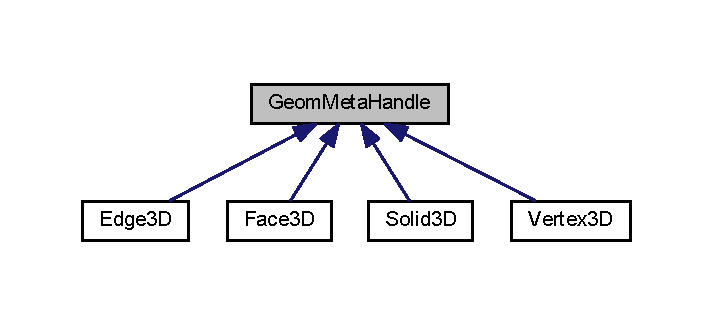
\includegraphics[width=342pt]{class_geom_meta_handle__inherit__graph}
\end{center}
\end{figure}
\subsection*{Public Member Functions}
\begin{DoxyCompactItemize}
\item 
\hypertarget{class_geom_meta_handle_a1787f612c3a943eda6368722713681f9}{\hyperlink{class_geom_meta_handle_a1787f612c3a943eda6368722713681f9}{Geom\-Meta\-Handle} ()}\label{class_geom_meta_handle_a1787f612c3a943eda6368722713681f9}

\begin{DoxyCompactList}\small\item\em Default constructor. Initialises values to null. \end{DoxyCompactList}\end{DoxyCompactItemize}
\subsection*{Public Attributes}
\begin{DoxyCompactItemize}
\item 
bool \hyperlink{class_geom_meta_handle_a545e915bdbffcafcf5cd9381b404874c}{m\-\_\-b\-Selected}
\end{DoxyCompactItemize}


\subsection{Detailed Description}
Metaclass which all geometry components subclass from. Contains useful metadata relevant to geometry components. 

\subsection{Member Data Documentation}
\hypertarget{class_geom_meta_handle_a545e915bdbffcafcf5cd9381b404874c}{\index{Geom\-Meta\-Handle@{Geom\-Meta\-Handle}!m\-\_\-b\-Selected@{m\-\_\-b\-Selected}}
\index{m\-\_\-b\-Selected@{m\-\_\-b\-Selected}!GeomMetaHandle@{Geom\-Meta\-Handle}}
\subsubsection[{m\-\_\-b\-Selected}]{\setlength{\rightskip}{0pt plus 5cm}bool Geom\-Meta\-Handle\-::m\-\_\-b\-Selected}}\label{class_geom_meta_handle_a545e915bdbffcafcf5cd9381b404874c}
Whether the component is currently selected. 

The documentation for this class was generated from the following file\-:\begin{DoxyCompactItemize}
\item 
app/\hyperlink{vertex_8h}{vertex.\-h}\end{DoxyCompactItemize}

\hypertarget{class_index_pool}{\section{Index\-Pool Class Reference}
\label{class_index_pool}\index{Index\-Pool@{Index\-Pool}}
}


The \hyperlink{class_index_pool}{Index\-Pool} class manages non-\/consecutive array indices.  




{\ttfamily \#include $<$indexpool.\-h$>$}



Inheritance diagram for Index\-Pool\-:\nopagebreak
\begin{figure}[H]
\begin{center}
\leavevmode
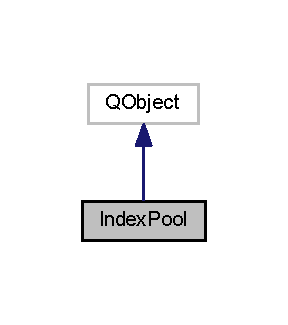
\includegraphics[width=138pt]{class_index_pool__inherit__graph}
\end{center}
\end{figure}


Collaboration diagram for Index\-Pool\-:\nopagebreak
\begin{figure}[H]
\begin{center}
\leavevmode
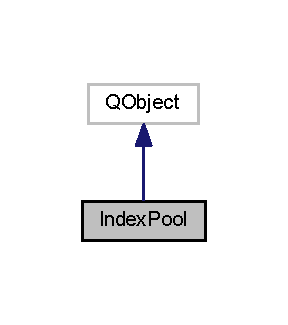
\includegraphics[width=138pt]{class_index_pool__coll__graph}
\end{center}
\end{figure}
\subsection*{Public Types}
\begin{DoxyCompactItemize}
\item 
enum \{ \hyperlink{class_index_pool_abacc88fb0ea6d1dcad5be70710ed0e3da3a3d6446453050cd4c95439b37b6824a}{I\-N\-D\-E\-X\-\_\-\-L\-I\-M\-I\-T} = 4294967294
 \}
\end{DoxyCompactItemize}
\subsection*{Public Slots}
\begin{DoxyCompactItemize}
\item 
void \hyperlink{class_index_pool_a7791b409b32242230867480c9b79de15}{release\-Index} (const \hyperlink{vertex_8h_a72202e57358ed73cd212e9a2eaf39aeb}{G\-E\-O\-M\-H\-A\-N\-D\-L\-E} index)
\begin{DoxyCompactList}\small\item\em Releases an index, allowing it to be allocated again. \end{DoxyCompactList}\item 
\hypertarget{class_index_pool_abda4a4fa05598f52c3af955788904c9f}{void \hyperlink{class_index_pool_abda4a4fa05598f52c3af955788904c9f}{condense} ()}\label{class_index_pool_abda4a4fa05598f52c3af955788904c9f}

\begin{DoxyCompactList}\small\item\em Condenses all indices (shifts indices down to fill all \char`\"{}holes\char`\"{} in the array). index\-Reallocation is fired for each re-\/allocated index. \end{DoxyCompactList}\end{DoxyCompactItemize}
\subsection*{Signals}
\begin{DoxyCompactItemize}
\item 
void \hyperlink{class_index_pool_a80b1499f90029a3531fc0603a5420cd8}{index\-Reallocation} (\hyperlink{vertex_8h_a72202e57358ed73cd212e9a2eaf39aeb}{G\-E\-O\-M\-H\-A\-N\-D\-L\-E} old\-Value, \hyperlink{vertex_8h_a72202e57358ed73cd212e9a2eaf39aeb}{G\-E\-O\-M\-H\-A\-N\-D\-L\-E} new\-Value)
\begin{DoxyCompactList}\small\item\em Fired when indices are re-\/allocated by \hyperlink{class_index_pool_abda4a4fa05598f52c3af955788904c9f}{condense()}. Any indices whose value does not get passed through this signal as old\-Value remains at its original value. \end{DoxyCompactList}\end{DoxyCompactItemize}
\subsection*{Public Member Functions}
\begin{DoxyCompactItemize}
\item 
\hyperlink{class_index_pool_a26e3c07764def73d6ebf8a1df0ce9bb4}{Index\-Pool} (Q\-Object $\ast$parent=0, \hyperlink{vertex_8h_a72202e57358ed73cd212e9a2eaf39aeb}{G\-E\-O\-M\-H\-A\-N\-D\-L\-E} highest\-Index=\hyperlink{class_index_pool_abacc88fb0ea6d1dcad5be70710ed0e3da3a3d6446453050cd4c95439b37b6824a}{I\-N\-D\-E\-X\-\_\-\-L\-I\-M\-I\-T})
\begin{DoxyCompactList}\small\item\em Constructor. \end{DoxyCompactList}\item 
bool \hyperlink{class_index_pool_a6001551942dde955048c7fdca82cbda7}{is\-Allocated} (\hyperlink{vertex_8h_a72202e57358ed73cd212e9a2eaf39aeb}{G\-E\-O\-M\-H\-A\-N\-D\-L\-E} index) const 
\begin{DoxyCompactList}\small\item\em Returns whether the specified index is currently allocated. \end{DoxyCompactList}\item 
bool \hyperlink{class_index_pool_a6f3dade75f8853215eb40b8dc9593f6c}{get\-Highest\-Allowed\-Index} () const 
\begin{DoxyCompactList}\small\item\em Returns the maximum index which can be allocated by this pool. \end{DoxyCompactList}\item 
\hyperlink{vertex_8h_a72202e57358ed73cd212e9a2eaf39aeb}{G\-E\-O\-M\-H\-A\-N\-D\-L\-E} \hyperlink{class_index_pool_a47301791c0015a14e7f459ae3efb614c}{allocate\-Index} ()
\begin{DoxyCompactList}\small\item\em Allocates the lowest free index. \end{DoxyCompactList}\end{DoxyCompactItemize}


\subsection{Detailed Description}
The \hyperlink{class_index_pool}{Index\-Pool} class manages non-\/consecutive array indices. 

The index pool works on the following heuristics\-:\par
 
\begin{DoxyItemize}
\item If the current number of allocated indices is contiguous (or nothing), the new index is allocated at the end of the current block of indices. 
\item If the current number of allocated indices is non-\/contiguous, the lowest unused index is allocated.
\end{DoxyItemize}\par
 This means that when indices are deallocated, \char`\"{}holes\char`\"{} in the array of indices are filled first before new indices are added to the end of the array. 

\subsection{Member Enumeration Documentation}
\hypertarget{class_index_pool_abacc88fb0ea6d1dcad5be70710ed0e3d}{\subsubsection[{anonymous enum}]{\setlength{\rightskip}{0pt plus 5cm}anonymous enum}}\label{class_index_pool_abacc88fb0ea6d1dcad5be70710ed0e3d}
\begin{Desc}
\item[Enumerator]\par
\begin{description}
\index{I\-N\-D\-E\-X\-\_\-\-L\-I\-M\-I\-T@{I\-N\-D\-E\-X\-\_\-\-L\-I\-M\-I\-T}!Index\-Pool@{Index\-Pool}}\index{Index\-Pool@{Index\-Pool}!I\-N\-D\-E\-X\-\_\-\-L\-I\-M\-I\-T@{I\-N\-D\-E\-X\-\_\-\-L\-I\-M\-I\-T}}\item[{\em 
\hypertarget{class_index_pool_abacc88fb0ea6d1dcad5be70710ed0e3da3a3d6446453050cd4c95439b37b6824a}{I\-N\-D\-E\-X\-\_\-\-L\-I\-M\-I\-T}\label{class_index_pool_abacc88fb0ea6d1dcad5be70710ed0e3da3a3d6446453050cd4c95439b37b6824a}
}]Highest allocatable index. \end{description}
\end{Desc}


\subsection{Constructor \& Destructor Documentation}
\hypertarget{class_index_pool_a26e3c07764def73d6ebf8a1df0ce9bb4}{\index{Index\-Pool@{Index\-Pool}!Index\-Pool@{Index\-Pool}}
\index{Index\-Pool@{Index\-Pool}!IndexPool@{Index\-Pool}}
\subsubsection[{Index\-Pool}]{\setlength{\rightskip}{0pt plus 5cm}Index\-Pool\-::\-Index\-Pool (
\begin{DoxyParamCaption}
\item[{Q\-Object $\ast$}]{parent = {\ttfamily 0}, }
\item[{{\bf G\-E\-O\-M\-H\-A\-N\-D\-L\-E}}]{highest\-Index = {\ttfamily {\bf I\-N\-D\-E\-X\-\_\-\-L\-I\-M\-I\-T}}}
\end{DoxyParamCaption}
)\hspace{0.3cm}{\ttfamily [explicit]}}}\label{class_index_pool_a26e3c07764def73d6ebf8a1df0ce9bb4}


Constructor. 


\begin{DoxyParams}{Parameters}
{\em parent} & Parent object. \\
\hline
{\em highest\-Index} & Highest number of indices. \\
\hline
\end{DoxyParams}


\subsection{Member Function Documentation}
\hypertarget{class_index_pool_a47301791c0015a14e7f459ae3efb614c}{\index{Index\-Pool@{Index\-Pool}!allocate\-Index@{allocate\-Index}}
\index{allocate\-Index@{allocate\-Index}!IndexPool@{Index\-Pool}}
\subsubsection[{allocate\-Index}]{\setlength{\rightskip}{0pt plus 5cm}{\bf G\-E\-O\-M\-H\-A\-N\-D\-L\-E} Index\-Pool\-::allocate\-Index (
\begin{DoxyParamCaption}
{}
\end{DoxyParamCaption}
)}}\label{class_index_pool_a47301791c0015a14e7f459ae3efb614c}


Allocates the lowest free index. 

\begin{DoxyReturn}{Returns}
Allocated index, or N\-U\-L\-L\-H\-N\-D if no more indices could be allocated. 
\end{DoxyReturn}
\hypertarget{class_index_pool_a6f3dade75f8853215eb40b8dc9593f6c}{\index{Index\-Pool@{Index\-Pool}!get\-Highest\-Allowed\-Index@{get\-Highest\-Allowed\-Index}}
\index{get\-Highest\-Allowed\-Index@{get\-Highest\-Allowed\-Index}!IndexPool@{Index\-Pool}}
\subsubsection[{get\-Highest\-Allowed\-Index}]{\setlength{\rightskip}{0pt plus 5cm}bool Index\-Pool\-::get\-Highest\-Allowed\-Index (
\begin{DoxyParamCaption}
{}
\end{DoxyParamCaption}
) const\hspace{0.3cm}{\ttfamily [inline]}}}\label{class_index_pool_a6f3dade75f8853215eb40b8dc9593f6c}


Returns the maximum index which can be allocated by this pool. 

\begin{DoxyReturn}{Returns}
Highest allowed index. 
\end{DoxyReturn}
\hypertarget{class_index_pool_a80b1499f90029a3531fc0603a5420cd8}{\index{Index\-Pool@{Index\-Pool}!index\-Reallocation@{index\-Reallocation}}
\index{index\-Reallocation@{index\-Reallocation}!IndexPool@{Index\-Pool}}
\subsubsection[{index\-Reallocation}]{\setlength{\rightskip}{0pt plus 5cm}void Index\-Pool\-::index\-Reallocation (
\begin{DoxyParamCaption}
\item[{{\bf G\-E\-O\-M\-H\-A\-N\-D\-L\-E}}]{old\-Value, }
\item[{{\bf G\-E\-O\-M\-H\-A\-N\-D\-L\-E}}]{new\-Value}
\end{DoxyParamCaption}
)\hspace{0.3cm}{\ttfamily [signal]}}}\label{class_index_pool_a80b1499f90029a3531fc0603a5420cd8}


Fired when indices are re-\/allocated by \hyperlink{class_index_pool_abda4a4fa05598f52c3af955788904c9f}{condense()}. Any indices whose value does not get passed through this signal as old\-Value remains at its original value. 


\begin{DoxyParams}{Parameters}
{\em old\-Value} & Old value of index. \\
\hline
{\em new\-Value} & The index's new value. \\
\hline
\end{DoxyParams}
\hypertarget{class_index_pool_a6001551942dde955048c7fdca82cbda7}{\index{Index\-Pool@{Index\-Pool}!is\-Allocated@{is\-Allocated}}
\index{is\-Allocated@{is\-Allocated}!IndexPool@{Index\-Pool}}
\subsubsection[{is\-Allocated}]{\setlength{\rightskip}{0pt plus 5cm}bool Index\-Pool\-::is\-Allocated (
\begin{DoxyParamCaption}
\item[{{\bf G\-E\-O\-M\-H\-A\-N\-D\-L\-E}}]{index}
\end{DoxyParamCaption}
) const}}\label{class_index_pool_a6001551942dde955048c7fdca82cbda7}


Returns whether the specified index is currently allocated. 


\begin{DoxyParams}{Parameters}
{\em index} & Index to check. \\
\hline
\end{DoxyParams}
\begin{DoxyReturn}{Returns}
True if already allocated, false if not. 
\end{DoxyReturn}
\hypertarget{class_index_pool_a7791b409b32242230867480c9b79de15}{\index{Index\-Pool@{Index\-Pool}!release\-Index@{release\-Index}}
\index{release\-Index@{release\-Index}!IndexPool@{Index\-Pool}}
\subsubsection[{release\-Index}]{\setlength{\rightskip}{0pt plus 5cm}void Index\-Pool\-::release\-Index (
\begin{DoxyParamCaption}
\item[{const {\bf G\-E\-O\-M\-H\-A\-N\-D\-L\-E}}]{index}
\end{DoxyParamCaption}
)\hspace{0.3cm}{\ttfamily [slot]}}}\label{class_index_pool_a7791b409b32242230867480c9b79de15}


Releases an index, allowing it to be allocated again. 


\begin{DoxyParams}{Parameters}
{\em index} & Index to release. \\
\hline
\end{DoxyParams}


The documentation for this class was generated from the following files\-:\begin{DoxyCompactItemize}
\item 
app/\hyperlink{indexpool_8h}{indexpool.\-h}\item 
app/indexpool.\-cpp\end{DoxyCompactItemize}

\hypertarget{class_i_vertex3_d_render_spec}{\section{I\-Vertex3\-D\-Render\-Spec Class Reference}
\label{class_i_vertex3_d_render_spec}\index{I\-Vertex3\-D\-Render\-Spec@{I\-Vertex3\-D\-Render\-Spec}}
}


Defines the properties required to be exposed by renderable vertices.  




{\ttfamily \#include $<$ivertex3drenderspec.\-h$>$}



Inheritance diagram for I\-Vertex3\-D\-Render\-Spec\-:
\nopagebreak
\begin{figure}[H]
\begin{center}
\leavevmode
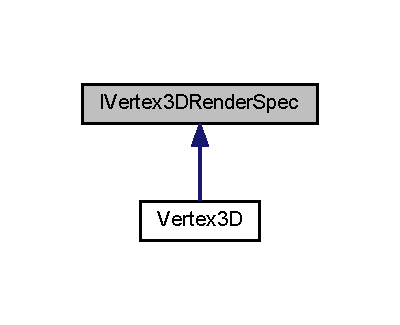
\includegraphics[width=192pt]{class_i_vertex3_d_render_spec__inherit__graph}
\end{center}
\end{figure}
\subsection*{Public Types}
\begin{DoxyCompactItemize}
\item 
enum \{ {\bfseries V3\-R\-S\-\_\-\-T\-O\-T\-A\-L\-\_\-\-D\-A\-T\-A\-\_\-\-T\-R\-A\-N\-S\-F\-E\-R} = 24
 \}
\end{DoxyCompactItemize}
\subsection*{Public Member Functions}
\begin{DoxyCompactItemize}
\item 
virtual unsigned long \hyperlink{class_i_vertex3_d_render_spec_a891d736d3d414de333398975f34bbae7}{V3\-R\-S\-\_\-\-Offset} ()=0
\begin{DoxyCompactList}\small\item\em Returns the offset of this vertex from the beginning of the V\-B\-O, in V3\-R\-S\-\_\-\-T\-O\-T\-A\-L\-\_\-\-D\-A\-T\-A\-\_\-\-T\-R\-A\-N\-S\-F\-E\-R steps. \end{DoxyCompactList}\item 
virtual void \hyperlink{class_i_vertex3_d_render_spec_a198bcfd0e8b6996848da0babe6805213}{V3\-R\-S\-\_\-\-Position} (float position\mbox{[}3\mbox{]})=0
\begin{DoxyCompactList}\small\item\em Fills an array with the position values for this vertex. \end{DoxyCompactList}\item 
virtual void \hyperlink{class_i_vertex3_d_render_spec_aaa32fb05761effc71596ee25c0eaaa77}{V3\-R\-S\-\_\-\-Colour} (unsigned char colour\mbox{[}4\mbox{]})=0
\begin{DoxyCompactList}\small\item\em Fills an array with the colour values for this vertex. \end{DoxyCompactList}\item 
virtual void \hyperlink{class_i_vertex3_d_render_spec_af9b255329a6ea9dd75e18699792b03e8}{V3\-R\-S\-\_\-\-Texture\-\_\-\-Coords} (float coords\mbox{[}2\mbox{]})=0
\begin{DoxyCompactList}\small\item\em Fills an array with the texture co-\/ordinate values for this vertex. \end{DoxyCompactList}\end{DoxyCompactItemize}


\subsection{Detailed Description}
Defines the properties required to be exposed by renderable vertices. 

\subsection{Member Function Documentation}
\hypertarget{class_i_vertex3_d_render_spec_aaa32fb05761effc71596ee25c0eaaa77}{\index{I\-Vertex3\-D\-Render\-Spec@{I\-Vertex3\-D\-Render\-Spec}!V3\-R\-S\-\_\-\-Colour@{V3\-R\-S\-\_\-\-Colour}}
\index{V3\-R\-S\-\_\-\-Colour@{V3\-R\-S\-\_\-\-Colour}!IVertex3DRenderSpec@{I\-Vertex3\-D\-Render\-Spec}}
\subsubsection[{V3\-R\-S\-\_\-\-Colour}]{\setlength{\rightskip}{0pt plus 5cm}virtual void I\-Vertex3\-D\-Render\-Spec\-::\-V3\-R\-S\-\_\-\-Colour (
\begin{DoxyParamCaption}
\item[{unsigned char}]{colour\mbox{[}4\mbox{]}}
\end{DoxyParamCaption}
)\hspace{0.3cm}{\ttfamily [pure virtual]}}}\label{class_i_vertex3_d_render_spec_aaa32fb05761effc71596ee25c0eaaa77}


Fills an array with the colour values for this vertex. 


\begin{DoxyParams}{Parameters}
{\em colour} & Colour values. Format is R\-G\-B\-A, range 0-\/255. \\
\hline
\end{DoxyParams}
\hypertarget{class_i_vertex3_d_render_spec_a891d736d3d414de333398975f34bbae7}{\index{I\-Vertex3\-D\-Render\-Spec@{I\-Vertex3\-D\-Render\-Spec}!V3\-R\-S\-\_\-\-Offset@{V3\-R\-S\-\_\-\-Offset}}
\index{V3\-R\-S\-\_\-\-Offset@{V3\-R\-S\-\_\-\-Offset}!IVertex3DRenderSpec@{I\-Vertex3\-D\-Render\-Spec}}
\subsubsection[{V3\-R\-S\-\_\-\-Offset}]{\setlength{\rightskip}{0pt plus 5cm}virtual unsigned long I\-Vertex3\-D\-Render\-Spec\-::\-V3\-R\-S\-\_\-\-Offset (
\begin{DoxyParamCaption}
{}
\end{DoxyParamCaption}
)\hspace{0.3cm}{\ttfamily [pure virtual]}}}\label{class_i_vertex3_d_render_spec_a891d736d3d414de333398975f34bbae7}


Returns the offset of this vertex from the beginning of the V\-B\-O, in V3\-R\-S\-\_\-\-T\-O\-T\-A\-L\-\_\-\-D\-A\-T\-A\-\_\-\-T\-R\-A\-N\-S\-F\-E\-R steps. 

\begin{DoxyReturn}{Returns}
Offset for this vertex. 
\end{DoxyReturn}


Implemented in \hyperlink{class_vertex3_d_a13a922fd8180591636c1daf4687cc205}{Vertex3\-D}.

\hypertarget{class_i_vertex3_d_render_spec_a198bcfd0e8b6996848da0babe6805213}{\index{I\-Vertex3\-D\-Render\-Spec@{I\-Vertex3\-D\-Render\-Spec}!V3\-R\-S\-\_\-\-Position@{V3\-R\-S\-\_\-\-Position}}
\index{V3\-R\-S\-\_\-\-Position@{V3\-R\-S\-\_\-\-Position}!IVertex3DRenderSpec@{I\-Vertex3\-D\-Render\-Spec}}
\subsubsection[{V3\-R\-S\-\_\-\-Position}]{\setlength{\rightskip}{0pt plus 5cm}virtual void I\-Vertex3\-D\-Render\-Spec\-::\-V3\-R\-S\-\_\-\-Position (
\begin{DoxyParamCaption}
\item[{float}]{position\mbox{[}3\mbox{]}}
\end{DoxyParamCaption}
)\hspace{0.3cm}{\ttfamily [pure virtual]}}}\label{class_i_vertex3_d_render_spec_a198bcfd0e8b6996848da0babe6805213}


Fills an array with the position values for this vertex. 


\begin{DoxyParams}{Parameters}
{\em position} & Array to fill. Format is X\-Y\-Z. \\
\hline
\end{DoxyParams}
\hypertarget{class_i_vertex3_d_render_spec_af9b255329a6ea9dd75e18699792b03e8}{\index{I\-Vertex3\-D\-Render\-Spec@{I\-Vertex3\-D\-Render\-Spec}!V3\-R\-S\-\_\-\-Texture\-\_\-\-Coords@{V3\-R\-S\-\_\-\-Texture\-\_\-\-Coords}}
\index{V3\-R\-S\-\_\-\-Texture\-\_\-\-Coords@{V3\-R\-S\-\_\-\-Texture\-\_\-\-Coords}!IVertex3DRenderSpec@{I\-Vertex3\-D\-Render\-Spec}}
\subsubsection[{V3\-R\-S\-\_\-\-Texture\-\_\-\-Coords}]{\setlength{\rightskip}{0pt plus 5cm}virtual void I\-Vertex3\-D\-Render\-Spec\-::\-V3\-R\-S\-\_\-\-Texture\-\_\-\-Coords (
\begin{DoxyParamCaption}
\item[{float}]{coords\mbox{[}2\mbox{]}}
\end{DoxyParamCaption}
)\hspace{0.3cm}{\ttfamily [pure virtual]}}}\label{class_i_vertex3_d_render_spec_af9b255329a6ea9dd75e18699792b03e8}


Fills an array with the texture co-\/ordinate values for this vertex. 


\begin{DoxyParams}{Parameters}
{\em coords} & Array to fill. Format is X\-Y. \\
\hline
\end{DoxyParams}


The documentation for this class was generated from the following file\-:\begin{DoxyCompactItemize}
\item 
app/\hyperlink{ivertex3drenderspec_8h}{ivertex3drenderspec.\-h}\end{DoxyCompactItemize}

\hypertarget{class_listed_command_manager}{\section{Listed\-Command\-Manager Class Reference}
\label{class_listed_command_manager}\index{Listed\-Command\-Manager@{Listed\-Command\-Manager}}
}


Inheritance diagram for Listed\-Command\-Manager\-:\nopagebreak
\begin{figure}[H]
\begin{center}
\leavevmode
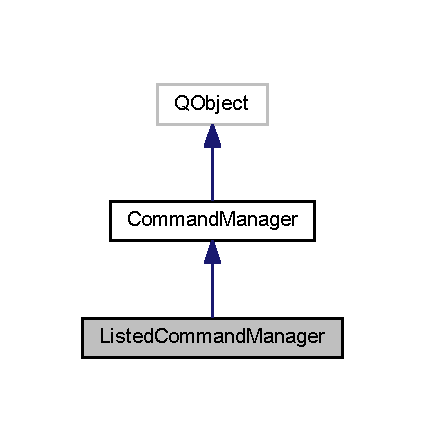
\includegraphics[width=204pt]{class_listed_command_manager__inherit__graph}
\end{center}
\end{figure}


Collaboration diagram for Listed\-Command\-Manager\-:\nopagebreak
\begin{figure}[H]
\begin{center}
\leavevmode
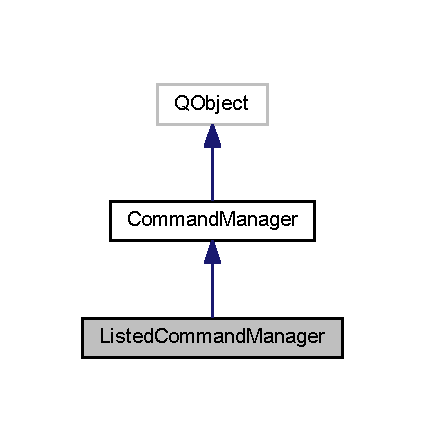
\includegraphics[width=204pt]{class_listed_command_manager__coll__graph}
\end{center}
\end{figure}
\subsection*{Public Member Functions}
\begin{DoxyCompactItemize}
\item 
\hypertarget{class_listed_command_manager_aeccd51549559c51c5e0e3b3e38c732e0}{{\bfseries Listed\-Command\-Manager} (Q\-Object $\ast$parent=0)}\label{class_listed_command_manager_aeccd51549559c51c5e0e3b3e38c732e0}

\item 
\hypertarget{class_listed_command_manager_a0d7559e6b7f8040dbcf58c6593e9f23c}{{\bfseries Listed\-Command\-Manager} (\hyperlink{class_listed_console_command}{Listed\-Console\-Command} $\ast$list\-Head, Q\-Object $\ast$parent=0)}\label{class_listed_command_manager_a0d7559e6b7f8040dbcf58c6593e9f23c}

\item 
\hypertarget{class_listed_command_manager_af10a37f7cd4adb7396e0a84f553aff21}{void {\bfseries traverse} (\hyperlink{class_listed_console_command}{Listed\-Console\-Command} $\ast$list\-Head)}\label{class_listed_command_manager_af10a37f7cd4adb7396e0a84f553aff21}

\end{DoxyCompactItemize}
\subsection*{Additional Inherited Members}


The documentation for this class was generated from the following files\-:\begin{DoxyCompactItemize}
\item 
I\-Console/inc/listedcommandmanager.\-h\item 
I\-Console/src/listedcommandmanager.\-cpp\end{DoxyCompactItemize}

\hypertarget{class_listed_console_command}{\section{Listed\-Console\-Command Class Reference}
\label{class_listed_console_command}\index{Listed\-Console\-Command@{Listed\-Console\-Command}}
}


Inheritance diagram for Listed\-Console\-Command\-:\nopagebreak
\begin{figure}[H]
\begin{center}
\leavevmode
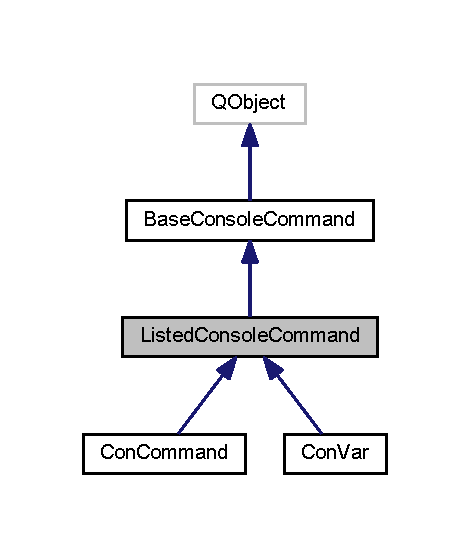
\includegraphics[width=225pt]{class_listed_console_command__inherit__graph}
\end{center}
\end{figure}


Collaboration diagram for Listed\-Console\-Command\-:\nopagebreak
\begin{figure}[H]
\begin{center}
\leavevmode
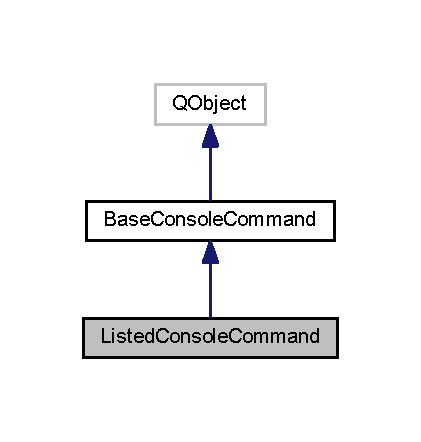
\includegraphics[width=202pt]{class_listed_console_command__coll__graph}
\end{center}
\end{figure}
\subsection*{Public Member Functions}
\begin{DoxyCompactItemize}
\item 
\hypertarget{class_listed_console_command_acbc2c1e24ef3fffd8d8f2b7d12b5b309}{{\bfseries Listed\-Console\-Command} (const Q\-String \&\hyperlink{class_base_console_command_a2f21764f46a3864a362eae2e3396e363}{name}, \hyperlink{class_command_manager}{Command\-Manager} $\ast$manager, \hyperlink{class_listed_console_command}{Listed\-Console\-Command} $\ast$$\ast$list\-Head, const Q\-String \&desc=\char`\"{}\char`\"{}, N\-Global\-Cmd\-::\-C\-M\-D\-F\-L\-A\-G\-S flags=0, Q\-Object $\ast$parent=0)}\label{class_listed_console_command_acbc2c1e24ef3fffd8d8f2b7d12b5b309}

\item 
\hypertarget{class_listed_console_command_a689a422172ced5156ba2b34ff1c2a800}{{\bfseries Listed\-Console\-Command} (const Q\-String \&\hyperlink{class_base_console_command_a2f21764f46a3864a362eae2e3396e363}{name}, const Q\-String \&desc=\char`\"{}\char`\"{}, N\-Global\-Cmd\-::\-C\-M\-D\-F\-L\-A\-G\-S flags=0, Q\-Object $\ast$parent=0)}\label{class_listed_console_command_a689a422172ced5156ba2b34ff1c2a800}

\item 
\hypertarget{class_listed_console_command_a84c311e9f2a70e9672b63f1da43ee0d2}{\hyperlink{class_listed_console_command}{Listed\-Console\-Command} $\ast$ {\bfseries get\-List\-Next} () const }\label{class_listed_console_command_a84c311e9f2a70e9672b63f1da43ee0d2}

\item 
\hypertarget{class_listed_console_command_ab14e1f1af33cef14d5a3b450ef44a31d}{void {\bfseries set\-List\-Next} (\hyperlink{class_listed_console_command}{Listed\-Console\-Command} $\ast$next)}\label{class_listed_console_command_ab14e1f1af33cef14d5a3b450ef44a31d}

\item 
\hypertarget{class_listed_console_command_a93828e08528c3a63811520369ea391db}{void {\bfseries try\-Register} (\hyperlink{class_command_manager}{Command\-Manager} $\ast$manager, \hyperlink{class_listed_console_command}{Listed\-Console\-Command} $\ast$$\ast$list\-Head)}\label{class_listed_console_command_a93828e08528c3a63811520369ea391db}

\end{DoxyCompactItemize}
\subsection*{Additional Inherited Members}


The documentation for this class was generated from the following files\-:\begin{DoxyCompactItemize}
\item 
I\-Console/inc/listedconsolecommand.\-h\item 
I\-Console/src/listedconsolecommand.\-cpp\end{DoxyCompactItemize}

\hypertarget{class_main_win}{\section{Main\-Win Class Reference}
\label{class_main_win}\index{Main\-Win@{Main\-Win}}
}


Application window class.  




{\ttfamily \#include $<$mainwin.\-h$>$}



Inheritance diagram for Main\-Win\-:\nopagebreak
\begin{figure}[H]
\begin{center}
\leavevmode
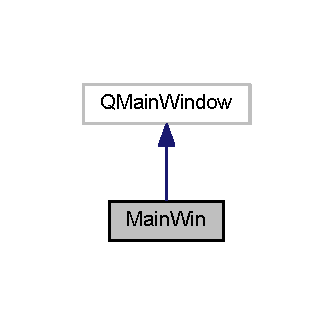
\includegraphics[width=160pt]{class_main_win__inherit__graph}
\end{center}
\end{figure}


Collaboration diagram for Main\-Win\-:\nopagebreak
\begin{figure}[H]
\begin{center}
\leavevmode
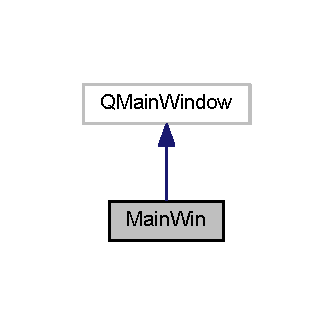
\includegraphics[width=160pt]{class_main_win__coll__graph}
\end{center}
\end{figure}
\subsection*{Public Member Functions}
\begin{DoxyCompactItemize}
\item 
\hypertarget{class_main_win_af05332e6fac4f7ab5c19b1a72aa7439d}{\hyperlink{class_main_win_af05332e6fac4f7ab5c19b1a72aa7439d}{Main\-Win} ()}\label{class_main_win_af05332e6fac4f7ab5c19b1a72aa7439d}

\begin{DoxyCompactList}\small\item\em Constructor. \end{DoxyCompactList}\item 
\hypertarget{class_main_win_a7068bb5ab02b75d4bbc78692388b9fb1}{\hyperlink{class_main_win_a7068bb5ab02b75d4bbc78692388b9fb1}{$\sim$\-Main\-Win} ()}\label{class_main_win_a7068bb5ab02b75d4bbc78692388b9fb1}

\begin{DoxyCompactList}\small\item\em Destructor. \end{DoxyCompactList}\item 
Q\-Size \hyperlink{class_main_win_af8f1854089c63efd6895ff536ad6ffc3}{size\-Hint} () const 
\begin{DoxyCompactList}\small\item\em Returns the desired size for when the window is created. \end{DoxyCompactList}\end{DoxyCompactItemize}
\subsection*{Protected Member Functions}
\begin{DoxyCompactItemize}
\item 
void \hyperlink{class_main_win_a06beabefe32c4e6514f76a07f1b63232}{close\-Event} (Q\-Close\-Event $\ast$event)
\begin{DoxyCompactList}\small\item\em Called when this window is closed\-: handles checking of log window. \end{DoxyCompactList}\end{DoxyCompactItemize}


\subsection{Detailed Description}
Application window class. 

Each \hyperlink{class_main_win}{Main\-Win} correcponds to exactly one currently open map document. If a new map document is created, it requires a new \hyperlink{class_main_win}{Main\-Win}. When the last \hyperlink{class_main_win}{Main\-Win} is closed, it will handle the closing of the log window if it is still open. 

\subsection{Member Function Documentation}
\hypertarget{class_main_win_a06beabefe32c4e6514f76a07f1b63232}{\index{Main\-Win@{Main\-Win}!close\-Event@{close\-Event}}
\index{close\-Event@{close\-Event}!MainWin@{Main\-Win}}
\subsubsection[{close\-Event}]{\setlength{\rightskip}{0pt plus 5cm}void Main\-Win\-::close\-Event (
\begin{DoxyParamCaption}
\item[{Q\-Close\-Event $\ast$}]{event}
\end{DoxyParamCaption}
)\hspace{0.3cm}{\ttfamily [protected]}}}\label{class_main_win_a06beabefe32c4e6514f76a07f1b63232}


Called when this window is closed\-: handles checking of log window. 


\begin{DoxyParams}{Parameters}
{\em event} & Close event. \\
\hline
\end{DoxyParams}
\hypertarget{class_main_win_af8f1854089c63efd6895ff536ad6ffc3}{\index{Main\-Win@{Main\-Win}!size\-Hint@{size\-Hint}}
\index{size\-Hint@{size\-Hint}!MainWin@{Main\-Win}}
\subsubsection[{size\-Hint}]{\setlength{\rightskip}{0pt plus 5cm}Q\-Size Main\-Win\-::size\-Hint (
\begin{DoxyParamCaption}
{}
\end{DoxyParamCaption}
) const\hspace{0.3cm}{\ttfamily [inline]}}}\label{class_main_win_af8f1854089c63efd6895ff536ad6ffc3}


Returns the desired size for when the window is created. 

\begin{DoxyReturn}{Returns}
Desired size. 
\end{DoxyReturn}


The documentation for this class was generated from the following files\-:\begin{DoxyCompactItemize}
\item 
app/\hyperlink{mainwin_8h}{mainwin.\-h}\item 
app/mainwin.\-cpp\end{DoxyCompactItemize}

\hypertarget{class_map_doc}{\section{Map\-Doc Class Reference}
\label{class_map_doc}\index{Map\-Doc@{Map\-Doc}}
}


The \hyperlink{class_map_doc}{Map\-Doc} class.  




{\ttfamily \#include $<$mapdoc.\-h$>$}



Inheritance diagram for Map\-Doc\-:
\nopagebreak
\begin{figure}[H]
\begin{center}
\leavevmode
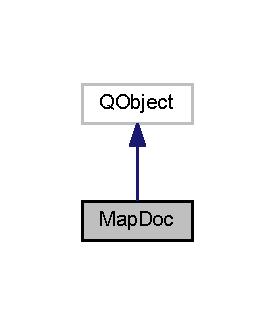
\includegraphics[width=132pt]{class_map_doc__inherit__graph}
\end{center}
\end{figure}


Collaboration diagram for Map\-Doc\-:
\nopagebreak
\begin{figure}[H]
\begin{center}
\leavevmode
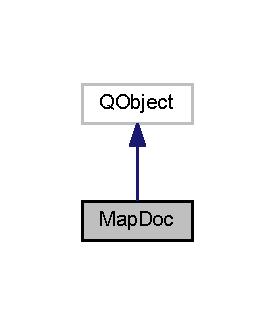
\includegraphics[width=132pt]{class_map_doc__coll__graph}
\end{center}
\end{figure}
\subsection*{Public Member Functions}
\begin{DoxyCompactItemize}
\item 
\hyperlink{class_map_doc_a2bea048c6b43333dc27fb4ca5ed84a95}{Map\-Doc} (Q\-Object $\ast$parent=0)
\begin{DoxyCompactList}\small\item\em Default constructor. \end{DoxyCompactList}\end{DoxyCompactItemize}
\subsection*{Static Public Member Functions}
\begin{DoxyCompactItemize}
\item 
static int \hyperlink{class_map_doc_a4bdaa5c5589e501d22a92f814f242b7c}{get\-Version} ()
\begin{DoxyCompactList}\small\item\em Gets the current version of the mapdoc. \end{DoxyCompactList}\end{DoxyCompactItemize}


\subsection{Detailed Description}
The \hyperlink{class_map_doc}{Map\-Doc} class. 

The \hyperlink{class_map_doc}{Map\-Doc} class details any information that will be serialised when a map source file is saved. This includes geometry and entities but also settings such as camera positions, grid size, snapping, etc. Geometry and entities are kept inside an octree that represents the entire 3\-D space in the level. 

\subsection{Constructor \& Destructor Documentation}
\hypertarget{class_map_doc_a2bea048c6b43333dc27fb4ca5ed84a95}{\index{Map\-Doc@{Map\-Doc}!Map\-Doc@{Map\-Doc}}
\index{Map\-Doc@{Map\-Doc}!MapDoc@{Map\-Doc}}
\subsubsection[{Map\-Doc}]{\setlength{\rightskip}{0pt plus 5cm}Map\-Doc\-::\-Map\-Doc (
\begin{DoxyParamCaption}
\item[{Q\-Object $\ast$}]{parent = {\ttfamily 0}}
\end{DoxyParamCaption}
)\hspace{0.3cm}{\ttfamily [explicit]}}}\label{class_map_doc_a2bea048c6b43333dc27fb4ca5ed84a95}


Default constructor. 


\begin{DoxyParams}{Parameters}
{\em parent} & Parent object. \\
\hline
\end{DoxyParams}


\subsection{Member Function Documentation}
\hypertarget{class_map_doc_a4bdaa5c5589e501d22a92f814f242b7c}{\index{Map\-Doc@{Map\-Doc}!get\-Version@{get\-Version}}
\index{get\-Version@{get\-Version}!MapDoc@{Map\-Doc}}
\subsubsection[{get\-Version}]{\setlength{\rightskip}{0pt plus 5cm}static int Map\-Doc\-::get\-Version (
\begin{DoxyParamCaption}
{}
\end{DoxyParamCaption}
)\hspace{0.3cm}{\ttfamily [inline]}, {\ttfamily [static]}}}\label{class_map_doc_a4bdaa5c5589e501d22a92f814f242b7c}


Gets the current version of the mapdoc. 

\begin{DoxyReturn}{Returns}
Mapdoc version. 
\end{DoxyReturn}


The documentation for this class was generated from the following files\-:\begin{DoxyCompactItemize}
\item 
app/\hyperlink{mapdoc_8h}{mapdoc.\-h}\item 
app/mapdoc.\-cpp\end{DoxyCompactItemize}

\hypertarget{class_plane}{\section{Plane Class Reference}
\label{class_plane}\index{Plane@{Plane}}
}


Defines a plane in 3\-D space.  




{\ttfamily \#include $<$plane.\-h$>$}

\subsection*{Public Member Functions}
\begin{DoxyCompactItemize}
\item 
\hypertarget{class_plane_acac0d9c003e0ab10d07b146c3566a0c7}{\hyperlink{class_plane_acac0d9c003e0ab10d07b146c3566a0c7}{Plane} ()}\label{class_plane_acac0d9c003e0ab10d07b146c3566a0c7}

\begin{DoxyCompactList}\small\item\em Constructor. Member variables are set to zero values. \end{DoxyCompactList}\item 
\hyperlink{class_plane_a044f4c5015112c8c5148ae28b41b8637}{Plane} (const Q\-Vector3\-D points\mbox{[}3\mbox{]})
\begin{DoxyCompactList}\small\item\em Constructor specifying an array of plane points. The normal is calculated with vectors \mbox{[}1\mbox{]}-\/\mbox{[}0\mbox{]}, \mbox{[}2\mbox{]}-\/\mbox{[}0\mbox{]}. \end{DoxyCompactList}\item 
\hyperlink{class_plane_affc3a1de45dcac9b65569eef3635eba4}{Plane} (const Q\-Vector3\-D p1, const Q\-Vector3\-D p2, const Q\-Vector3\-D p3)
\begin{DoxyCompactList}\small\item\em Constructor specifying plane points. The normal is calculated with vectors p2-\/p1, p3-\/p1. \end{DoxyCompactList}\item 
void \hyperlink{class_plane_af04d6d582cfc6bb3fdebfb7d2711c0b8}{get\-Points} (Q\-Vector3\-D points\mbox{[}3\mbox{]}) const 
\begin{DoxyCompactList}\small\item\em Gets an array of the three points on the plane. \end{DoxyCompactList}\item 
void \hyperlink{class_plane_ad8ca5183fed9db77a2cbb552d780aa9d}{get\-Points} (Q\-List$<$ Q\-Vector3\-D $>$ \&points) const 
\begin{DoxyCompactList}\small\item\em Fills a Q\-List with the three points on the plane. \end{DoxyCompactList}\item 
bool \hyperlink{class_plane_a9324f303beccf7ec9c6d3a5e371b7ca7}{is\-Valid} () const 
\begin{DoxyCompactList}\small\item\em Specifies whether the plane is valid. Invalid planes contain two or more identical plane points. \end{DoxyCompactList}\item 
Q\-Vector3\-D \hyperlink{class_plane_aeaae7bd417894c587423251818f16197}{get\-Normal} () const 
\begin{DoxyCompactList}\small\item\em Returns the plane's normal, specifying the forward-\/facing direction of the plane. \end{DoxyCompactList}\item 
void \hyperlink{class_plane_a3a9fd7ef1b74fad45bf0b18b93922813}{set\-Points} (const Q\-Vector3\-D points\mbox{[}3\mbox{]})
\begin{DoxyCompactList}\small\item\em Sets the plane's points via an array. The normal is calculated with vectors \mbox{[}1\mbox{]}-\/\mbox{[}0\mbox{]}, \mbox{[}2\mbox{]}-\/\mbox{[}0\mbox{]}. \end{DoxyCompactList}\item 
void \hyperlink{class_plane_ae4c5f7cda6d296b3cfccaac102471098}{set\-Points} (const Q\-List$<$ Q\-Vector3\-D $>$ \&points)
\begin{DoxyCompactList}\small\item\em Sets the plane's points via a Q\-List. The normal is calculated with vectors \mbox{[}1\mbox{]}-\/\mbox{[}0\mbox{]}, \mbox{[}2\mbox{]}-\/\mbox{[}0\mbox{]}. \end{DoxyCompactList}\item 
void \hyperlink{class_plane_a99ba0636ee74ea4cd8e5da15145b7c42}{set\-Points} (const Q\-Vector3\-D p1, const Q\-Vector3\-D p2, const Q\-Vector3\-D p3)
\begin{DoxyCompactList}\small\item\em Sets the plane's points. The normal is calculated with vectors p2-\/p1, p3-\/p1. \end{DoxyCompactList}\end{DoxyCompactItemize}


\subsection{Detailed Description}
Defines a plane in 3\-D space. 

\subsection{Constructor \& Destructor Documentation}
\hypertarget{class_plane_a044f4c5015112c8c5148ae28b41b8637}{\index{Plane@{Plane}!Plane@{Plane}}
\index{Plane@{Plane}!Plane@{Plane}}
\subsubsection[{Plane}]{\setlength{\rightskip}{0pt plus 5cm}Plane\-::\-Plane (
\begin{DoxyParamCaption}
\item[{const Q\-Vector3\-D}]{points\mbox{[}3\mbox{]}}
\end{DoxyParamCaption}
)\hspace{0.3cm}{\ttfamily [inline]}}}\label{class_plane_a044f4c5015112c8c5148ae28b41b8637}


Constructor specifying an array of plane points. The normal is calculated with vectors \mbox{[}1\mbox{]}-\/\mbox{[}0\mbox{]}, \mbox{[}2\mbox{]}-\/\mbox{[}0\mbox{]}. 


\begin{DoxyParams}{Parameters}
{\em points} & 3 points on the plane. \\
\hline
\end{DoxyParams}
\hypertarget{class_plane_affc3a1de45dcac9b65569eef3635eba4}{\index{Plane@{Plane}!Plane@{Plane}}
\index{Plane@{Plane}!Plane@{Plane}}
\subsubsection[{Plane}]{\setlength{\rightskip}{0pt plus 5cm}Plane\-::\-Plane (
\begin{DoxyParamCaption}
\item[{const Q\-Vector3\-D}]{p1, }
\item[{const Q\-Vector3\-D}]{p2, }
\item[{const Q\-Vector3\-D}]{p3}
\end{DoxyParamCaption}
)\hspace{0.3cm}{\ttfamily [inline]}}}\label{class_plane_affc3a1de45dcac9b65569eef3635eba4}


Constructor specifying plane points. The normal is calculated with vectors p2-\/p1, p3-\/p1. 


\begin{DoxyParams}{Parameters}
{\em p1} & Point 1. \\
\hline
{\em p2} & Point 2. \\
\hline
{\em p3} & Point 3. \\
\hline
\end{DoxyParams}


\subsection{Member Function Documentation}
\hypertarget{class_plane_aeaae7bd417894c587423251818f16197}{\index{Plane@{Plane}!get\-Normal@{get\-Normal}}
\index{get\-Normal@{get\-Normal}!Plane@{Plane}}
\subsubsection[{get\-Normal}]{\setlength{\rightskip}{0pt plus 5cm}Q\-Vector3\-D Plane\-::get\-Normal (
\begin{DoxyParamCaption}
{}
\end{DoxyParamCaption}
) const\hspace{0.3cm}{\ttfamily [inline]}}}\label{class_plane_aeaae7bd417894c587423251818f16197}


Returns the plane's normal, specifying the forward-\/facing direction of the plane. 

\begin{DoxyReturn}{Returns}
Normalised direction vector representing the plane's normal. 
\end{DoxyReturn}
\hypertarget{class_plane_af04d6d582cfc6bb3fdebfb7d2711c0b8}{\index{Plane@{Plane}!get\-Points@{get\-Points}}
\index{get\-Points@{get\-Points}!Plane@{Plane}}
\subsubsection[{get\-Points}]{\setlength{\rightskip}{0pt plus 5cm}void Plane\-::get\-Points (
\begin{DoxyParamCaption}
\item[{Q\-Vector3\-D}]{points\mbox{[}3\mbox{]}}
\end{DoxyParamCaption}
) const\hspace{0.3cm}{\ttfamily [inline]}}}\label{class_plane_af04d6d582cfc6bb3fdebfb7d2711c0b8}


Gets an array of the three points on the plane. 


\begin{DoxyParams}{Parameters}
{\em points} & Array to fill with points. \\
\hline
\end{DoxyParams}
\hypertarget{class_plane_ad8ca5183fed9db77a2cbb552d780aa9d}{\index{Plane@{Plane}!get\-Points@{get\-Points}}
\index{get\-Points@{get\-Points}!Plane@{Plane}}
\subsubsection[{get\-Points}]{\setlength{\rightskip}{0pt plus 5cm}void Plane\-::get\-Points (
\begin{DoxyParamCaption}
\item[{Q\-List$<$ Q\-Vector3\-D $>$ \&}]{points}
\end{DoxyParamCaption}
) const\hspace{0.3cm}{\ttfamily [inline]}}}\label{class_plane_ad8ca5183fed9db77a2cbb552d780aa9d}


Fills a Q\-List with the three points on the plane. 


\begin{DoxyParams}{Parameters}
{\em points} & List to fill. Points are appended to the list. \\
\hline
\end{DoxyParams}
\hypertarget{class_plane_a9324f303beccf7ec9c6d3a5e371b7ca7}{\index{Plane@{Plane}!is\-Valid@{is\-Valid}}
\index{is\-Valid@{is\-Valid}!Plane@{Plane}}
\subsubsection[{is\-Valid}]{\setlength{\rightskip}{0pt plus 5cm}bool Plane\-::is\-Valid (
\begin{DoxyParamCaption}
{}
\end{DoxyParamCaption}
) const\hspace{0.3cm}{\ttfamily [inline]}}}\label{class_plane_a9324f303beccf7ec9c6d3a5e371b7ca7}


Specifies whether the plane is valid. Invalid planes contain two or more identical plane points. 

\begin{DoxyReturn}{Returns}
True if valid, false otherwise. 
\end{DoxyReturn}
\hypertarget{class_plane_a3a9fd7ef1b74fad45bf0b18b93922813}{\index{Plane@{Plane}!set\-Points@{set\-Points}}
\index{set\-Points@{set\-Points}!Plane@{Plane}}
\subsubsection[{set\-Points}]{\setlength{\rightskip}{0pt plus 5cm}void Plane\-::set\-Points (
\begin{DoxyParamCaption}
\item[{const Q\-Vector3\-D}]{points\mbox{[}3\mbox{]}}
\end{DoxyParamCaption}
)}}\label{class_plane_a3a9fd7ef1b74fad45bf0b18b93922813}


Sets the plane's points via an array. The normal is calculated with vectors \mbox{[}1\mbox{]}-\/\mbox{[}0\mbox{]}, \mbox{[}2\mbox{]}-\/\mbox{[}0\mbox{]}. 


\begin{DoxyParams}{Parameters}
{\em points} & Array of points to set. \\
\hline
\end{DoxyParams}
\hypertarget{class_plane_ae4c5f7cda6d296b3cfccaac102471098}{\index{Plane@{Plane}!set\-Points@{set\-Points}}
\index{set\-Points@{set\-Points}!Plane@{Plane}}
\subsubsection[{set\-Points}]{\setlength{\rightskip}{0pt plus 5cm}void Plane\-::set\-Points (
\begin{DoxyParamCaption}
\item[{const Q\-List$<$ Q\-Vector3\-D $>$ \&}]{points}
\end{DoxyParamCaption}
)}}\label{class_plane_ae4c5f7cda6d296b3cfccaac102471098}


Sets the plane's points via a Q\-List. The normal is calculated with vectors \mbox{[}1\mbox{]}-\/\mbox{[}0\mbox{]}, \mbox{[}2\mbox{]}-\/\mbox{[}0\mbox{]}. 


\begin{DoxyParams}{Parameters}
{\em points} & List of points to set. \\
\hline
\end{DoxyParams}
\hypertarget{class_plane_a99ba0636ee74ea4cd8e5da15145b7c42}{\index{Plane@{Plane}!set\-Points@{set\-Points}}
\index{set\-Points@{set\-Points}!Plane@{Plane}}
\subsubsection[{set\-Points}]{\setlength{\rightskip}{0pt plus 5cm}void Plane\-::set\-Points (
\begin{DoxyParamCaption}
\item[{const Q\-Vector3\-D}]{p1, }
\item[{const Q\-Vector3\-D}]{p2, }
\item[{const Q\-Vector3\-D}]{p3}
\end{DoxyParamCaption}
)}}\label{class_plane_a99ba0636ee74ea4cd8e5da15145b7c42}


Sets the plane's points. The normal is calculated with vectors p2-\/p1, p3-\/p1. 


\begin{DoxyParams}{Parameters}
{\em p1} & First point. \\
\hline
{\em p2} & Second point. \\
\hline
{\em p3} & Third point. \\
\hline
\end{DoxyParams}


The documentation for this class was generated from the following files\-:\begin{DoxyCompactItemize}
\item 
app/\hyperlink{plane_8h}{plane.\-h}\item 
app/plane.\-cpp\end{DoxyCompactItemize}

\hypertarget{class_solid3_d}{\section{Solid3\-D Class Reference}
\label{class_solid3_d}\index{Solid3\-D@{Solid3\-D}}
}


Class representing a 3\-D solid.  




{\ttfamily \#include $<$solid.\-h$>$}



Inheritance diagram for Solid3\-D\-:\nopagebreak
\begin{figure}[H]
\begin{center}
\leavevmode
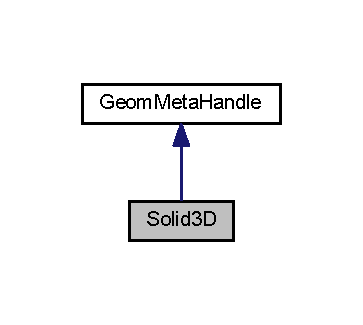
\includegraphics[width=174pt]{class_solid3_d__inherit__graph}
\end{center}
\end{figure}


Collaboration diagram for Solid3\-D\-:\nopagebreak
\begin{figure}[H]
\begin{center}
\leavevmode
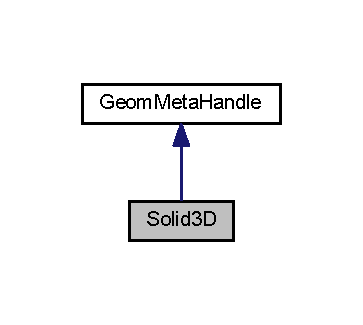
\includegraphics[width=174pt]{class_solid3_d__coll__graph}
\end{center}
\end{figure}
\subsection*{Public Types}
\begin{DoxyCompactItemize}
\item 
enum \{ \hyperlink{class_solid3_d_a85c6b265036f308d59f14a1945419de3a0bc5c527e2f2681822af8cdbe91f13cb}{M\-A\-X\-\_\-\-V\-E\-R\-T\-I\-C\-E\-S} = 384, 
\hyperlink{class_solid3_d_a85c6b265036f308d59f14a1945419de3adea5e83841760466066bb7ef63f9779f}{M\-A\-X\-\_\-\-E\-D\-G\-E\-S} = 384, 
\hyperlink{class_solid3_d_a85c6b265036f308d59f14a1945419de3a85c95a8842482e9e0db2f3c6ff68f19a}{M\-A\-X\-\_\-\-F\-A\-C\-E\-S} = 384
 \}
\item 
\hypertarget{class_solid3_d_acaa1c40fc6c74ee5c77e64baa3a672b1}{typedef Q\-Vector$<$ \hyperlink{class_vertex3_d}{Vertex3\-D} $\ast$ $>$ \hyperlink{class_solid3_d_acaa1c40fc6c74ee5c77e64baa3a672b1}{Vertex3\-D\-List}}\label{class_solid3_d_acaa1c40fc6c74ee5c77e64baa3a672b1}

\begin{DoxyCompactList}\small\item\em Vertex3\-D\-List typedef. \end{DoxyCompactList}\item 
\hypertarget{class_solid3_d_ac9b57b2279aeedb1dc657ac13271727b}{typedef Q\-Vector$<$ \hyperlink{class_edge3_d}{Edge3\-D} $\ast$ $>$ \hyperlink{class_solid3_d_ac9b57b2279aeedb1dc657ac13271727b}{Edge3\-D\-List}}\label{class_solid3_d_ac9b57b2279aeedb1dc657ac13271727b}

\begin{DoxyCompactList}\small\item\em Edge3\-D\-List typedef. \end{DoxyCompactList}\item 
\hypertarget{class_solid3_d_afd4862e0f4b30967e6f0cb2013ccc084}{typedef Q\-Vector$<$ \hyperlink{class_face3_d}{Face3\-D} $\ast$ $>$ \hyperlink{class_solid3_d_afd4862e0f4b30967e6f0cb2013ccc084}{Face3\-D\-List}}\label{class_solid3_d_afd4862e0f4b30967e6f0cb2013ccc084}

\begin{DoxyCompactList}\small\item\em Face3\-D\-List typedef. \end{DoxyCompactList}\end{DoxyCompactItemize}
\subsection*{Public Member Functions}
\begin{DoxyCompactItemize}
\item 
\hypertarget{class_solid3_d_a8c69dd01b422d74c8ff298e7f9ba95d5}{\hyperlink{class_solid3_d_a8c69dd01b422d74c8ff298e7f9ba95d5}{Solid3\-D} ()}\label{class_solid3_d_a8c69dd01b422d74c8ff298e7f9ba95d5}

\begin{DoxyCompactList}\small\item\em Default constructor. Initialises empty members. \end{DoxyCompactList}\item 
\hypertarget{class_solid3_d_afa6ecd2e276b4ef5a09f3c660a6ccfed}{\hyperlink{class_solid3_d_afa6ecd2e276b4ef5a09f3c660a6ccfed}{$\sim$\-Solid3\-D} ()}\label{class_solid3_d_afa6ecd2e276b4ef5a09f3c660a6ccfed}

\begin{DoxyCompactList}\small\item\em Destructor. \end{DoxyCompactList}\item 
bool \hyperlink{class_solid3_d_ac02ad8ea1ca4d970c77ddc4c09b043cc}{add\-Vertex} (\hyperlink{class_vertex3_d}{Vertex3\-D} $\ast$vertex)
\begin{DoxyCompactList}\small\item\em Adds the specified vertex. \end{DoxyCompactList}\item 
\hyperlink{class_vertex3_d}{Vertex3\-D} $\ast$ \hyperlink{class_solid3_d_aefadc03bef752b5eeb52e80d67074980}{remove\-Vertex\-Handle} (const \hyperlink{vertex_8h_a72202e57358ed73cd212e9a2eaf39aeb}{G\-E\-O\-M\-H\-A\-N\-D\-L\-E} vertex)
\begin{DoxyCompactList}\small\item\em Removes the vertex with the specified handle. \end{DoxyCompactList}\item 
\hyperlink{class_vertex3_d}{Vertex3\-D} $\ast$ \hyperlink{class_solid3_d_ace3ab2ef41ff561973c10253b18add81}{find\-Vertex} (const \hyperlink{vertex_8h_a72202e57358ed73cd212e9a2eaf39aeb}{G\-E\-O\-M\-H\-A\-N\-D\-L\-E} vertex) const 
\begin{DoxyCompactList}\small\item\em Returns a pointer to the vertex with the specified handle. \end{DoxyCompactList}\item 
void \hyperlink{class_solid3_d_aa250bf5e45c3890a031ee7d10fd0a495}{find\-Related\-Edges\-For\-Vertex} (Q\-List$<$ \hyperlink{vertex_8h_a72202e57358ed73cd212e9a2eaf39aeb}{G\-E\-O\-M\-H\-A\-N\-D\-L\-E} $>$ \&out\-Edges, \hyperlink{vertex_8h_a72202e57358ed73cd212e9a2eaf39aeb}{G\-E\-O\-M\-H\-A\-N\-D\-L\-E} vertex)
\begin{DoxyCompactList}\small\item\em Finds all edges whose start or end vertices reference the given vertex handle. \end{DoxyCompactList}\item 
void \hyperlink{class_solid3_d_a84f5c532f14916e59ba99b339e19975e}{find\-Related\-Edges\-For\-Vertex} (Q\-List$<$ \hyperlink{vertex_8h_a72202e57358ed73cd212e9a2eaf39aeb}{G\-E\-O\-M\-H\-A\-N\-D\-L\-E} $>$ \&out\-Edges, Q\-List$<$ \hyperlink{vertex_8h_a72202e57358ed73cd212e9a2eaf39aeb}{G\-E\-O\-M\-H\-A\-N\-D\-L\-E} $>$ \&vertices)
\begin{DoxyCompactList}\small\item\em Finds all edges whose start or end vertices reference any of the given vertex handles. \end{DoxyCompactList}\item 
void \hyperlink{class_solid3_d_a00bfad9d7e6dbe5ff290074753329e92}{find\-Related\-Faces\-For\-Vertex} (Q\-List$<$ \hyperlink{vertex_8h_a72202e57358ed73cd212e9a2eaf39aeb}{G\-E\-O\-M\-H\-A\-N\-D\-L\-E} $>$ \&out\-Faces, \hyperlink{vertex_8h_a72202e57358ed73cd212e9a2eaf39aeb}{G\-E\-O\-M\-H\-A\-N\-D\-L\-E} vertex)
\begin{DoxyCompactList}\small\item\em Finds all faces whose edges reference the given vertex handle. \end{DoxyCompactList}\item 
void \hyperlink{class_solid3_d_ac2b735d2b9ee6e47f56b49e4b122582c}{find\-Related\-Faces\-For\-Vertex} (Q\-List$<$ \hyperlink{vertex_8h_a72202e57358ed73cd212e9a2eaf39aeb}{G\-E\-O\-M\-H\-A\-N\-D\-L\-E} $>$ \&out\-Faces, Q\-List$<$ \hyperlink{vertex_8h_a72202e57358ed73cd212e9a2eaf39aeb}{G\-E\-O\-M\-H\-A\-N\-D\-L\-E} $>$ \&vertices)
\begin{DoxyCompactList}\small\item\em Finds all faces whose edges reference any of the given vertex handles. \end{DoxyCompactList}\item 
bool \hyperlink{class_solid3_d_aad6d7269dbea23a025ba3f598183bc22}{add\-Edge} (\hyperlink{class_edge3_d}{Edge3\-D} $\ast$edge)
\begin{DoxyCompactList}\small\item\em Adds the specified edge. \end{DoxyCompactList}\item 
\hyperlink{class_edge3_d}{Edge3\-D} $\ast$ \hyperlink{class_solid3_d_a3874333554e5105e789e06de3accb9d5}{remove\-Edge\-Handle} (const \hyperlink{vertex_8h_a72202e57358ed73cd212e9a2eaf39aeb}{G\-E\-O\-M\-H\-A\-N\-D\-L\-E} edge)
\begin{DoxyCompactList}\small\item\em Removes the edge with the specified handle. \end{DoxyCompactList}\item 
\hyperlink{class_edge3_d}{Edge3\-D} $\ast$ \hyperlink{class_solid3_d_ab5a26fa3df1a830f972bd3a57d412a08}{find\-Edge} (const \hyperlink{vertex_8h_a72202e57358ed73cd212e9a2eaf39aeb}{G\-E\-O\-M\-H\-A\-N\-D\-L\-E} edge) const 
\begin{DoxyCompactList}\small\item\em Returns a pointer to the edge with the specified handle. \end{DoxyCompactList}\item 
void \hyperlink{class_solid3_d_a3a7ce9251333f2ff387292d229ac4aa5}{find\-Related\-Faces\-For\-Edge} (Q\-List$<$ \hyperlink{vertex_8h_a72202e57358ed73cd212e9a2eaf39aeb}{G\-E\-O\-M\-H\-A\-N\-D\-L\-E} $>$ \&out\-Faces, \hyperlink{vertex_8h_a72202e57358ed73cd212e9a2eaf39aeb}{G\-E\-O\-M\-H\-A\-N\-D\-L\-E} edge)
\begin{DoxyCompactList}\small\item\em Finds all faces which contain the given edge. \end{DoxyCompactList}\item 
void \hyperlink{class_solid3_d_aa388640fa5cf2fb0e94630f5480f024e}{find\-Related\-Faces\-For\-Edge} (Q\-List$<$ \hyperlink{vertex_8h_a72202e57358ed73cd212e9a2eaf39aeb}{G\-E\-O\-M\-H\-A\-N\-D\-L\-E} $>$ \&out\-Faces, Q\-List$<$ \hyperlink{vertex_8h_a72202e57358ed73cd212e9a2eaf39aeb}{G\-E\-O\-M\-H\-A\-N\-D\-L\-E} $>$ \&edges)
\begin{DoxyCompactList}\small\item\em Finds all faces which contain any of the given edges. \end{DoxyCompactList}\item 
bool \hyperlink{class_solid3_d_a3976c227473c5954bfac9e2edf4078ea}{add\-Face} (\hyperlink{class_face3_d}{Face3\-D} $\ast$face)
\begin{DoxyCompactList}\small\item\em Adds the specified face. \end{DoxyCompactList}\item 
\hyperlink{class_face3_d}{Face3\-D} $\ast$ \hyperlink{class_solid3_d_a49bec433727595c0aa5fef4097e9d6b2}{remove\-Face\-Handle} (const \hyperlink{vertex_8h_a72202e57358ed73cd212e9a2eaf39aeb}{G\-E\-O\-M\-H\-A\-N\-D\-L\-E} face)
\begin{DoxyCompactList}\small\item\em Removes the face with the specified handle. \end{DoxyCompactList}\item 
\hyperlink{class_face3_d}{Face3\-D} $\ast$ \hyperlink{class_solid3_d_af1e9c9e9c969f7f935296c3706e8f08f}{find\-Face} (const \hyperlink{vertex_8h_a72202e57358ed73cd212e9a2eaf39aeb}{G\-E\-O\-M\-H\-A\-N\-D\-L\-E} face) const 
\begin{DoxyCompactList}\small\item\em Returns a pointer to the face with the specified handle. \end{DoxyCompactList}\item 
void \hyperlink{class_solid3_d_a844ed140f035f5cbeb325687d10e9d32}{identify\-Handle} (\hyperlink{vertex_8h_a72202e57358ed73cd212e9a2eaf39aeb}{G\-E\-O\-M\-H\-A\-N\-D\-L\-E} handle, \hyperlink{struct_geom_info}{Geom\-Info} \&info) const 
\begin{DoxyCompactList}\small\item\em Outputs information about the given geometry component to the \hyperlink{struct_geom_info}{Geom\-Info} struct. \end{DoxyCompactList}\item 
const \hyperlink{class_solid3_d_acaa1c40fc6c74ee5c77e64baa3a672b1}{Vertex3\-D\-List} \& \hyperlink{class_solid3_d_aa97775f007b84f89802d1f87b24665a0}{get\-Vertex\-List} () const 
\begin{DoxyCompactList}\small\item\em Returns the vertex list. \end{DoxyCompactList}\item 
const \hyperlink{class_solid3_d_ac9b57b2279aeedb1dc657ac13271727b}{Edge3\-D\-List} \& \hyperlink{class_solid3_d_ab0937f1a2d79a4ae72fcafb7b9f4ab7d}{get\-Edge\-List} () const 
\begin{DoxyCompactList}\small\item\em Returns the edge list. \end{DoxyCompactList}\item 
const \hyperlink{class_solid3_d_afd4862e0f4b30967e6f0cb2013ccc084}{Face3\-D\-List} \& \hyperlink{class_solid3_d_a17968c6a8e59d14268240ff1548cc51d}{get\-Face\-List} () const 
\begin{DoxyCompactList}\small\item\em Returns the face list. \end{DoxyCompactList}\item 
\hyperlink{vertex_8h_a72202e57358ed73cd212e9a2eaf39aeb}{G\-E\-O\-M\-H\-A\-N\-D\-L\-E} \hyperlink{class_solid3_d_ac2fda07777d7c7a856add07ceb24c395}{get\-Handle} () const 
\begin{DoxyCompactList}\small\item\em Returns this solid's handle. \end{DoxyCompactList}\item 
void \hyperlink{class_solid3_d_ab12674813ab277a7c4dac092367da6cd}{set\-Handle} (const \hyperlink{vertex_8h_a72202e57358ed73cd212e9a2eaf39aeb}{G\-E\-O\-M\-H\-A\-N\-D\-L\-E} handle)
\begin{DoxyCompactList}\small\item\em Sets this solid's handle. \end{DoxyCompactList}\end{DoxyCompactItemize}
\subsection*{Additional Inherited Members}


\subsection{Detailed Description}
Class representing a 3\-D solid. 

Solids are the programmatical implementation of brushes and are made up of sets of vertices, edges and faces. Each edge references the vertices it links, and each face is built from multiple edges. As opposed to Hammer's implementation, solids are mesh-\/based (ie. they are defined by vertex positions and links rather than planes and intersections) to allow for easier manipulation, and are exported as plane-\/based objects when serialised as a V\-M\-F.\par
 It is recommended to work {\bfseries bottom-\/up} (ie. add any required vertices before edges, and edges before faces) rather than {\bfseries top-\/down} (creating all of a face's edges and vertices as the face itself is created) as the former method is less prone to errors. 

\subsection{Member Enumeration Documentation}
\hypertarget{class_solid3_d_a85c6b265036f308d59f14a1945419de3}{\subsubsection[{anonymous enum}]{\setlength{\rightskip}{0pt plus 5cm}anonymous enum}}\label{class_solid3_d_a85c6b265036f308d59f14a1945419de3}
\begin{Desc}
\item[Enumerator]\par
\begin{description}
\index{M\-A\-X\-\_\-\-V\-E\-R\-T\-I\-C\-E\-S@{M\-A\-X\-\_\-\-V\-E\-R\-T\-I\-C\-E\-S}!Solid3\-D@{Solid3\-D}}\index{Solid3\-D@{Solid3\-D}!M\-A\-X\-\_\-\-V\-E\-R\-T\-I\-C\-E\-S@{M\-A\-X\-\_\-\-V\-E\-R\-T\-I\-C\-E\-S}}\item[{\em 
\hypertarget{class_solid3_d_a85c6b265036f308d59f14a1945419de3a0bc5c527e2f2681822af8cdbe91f13cb}{M\-A\-X\-\_\-\-V\-E\-R\-T\-I\-C\-E\-S}\label{class_solid3_d_a85c6b265036f308d59f14a1945419de3a0bc5c527e2f2681822af8cdbe91f13cb}
}]Max vertices allowed in a solid. \index{M\-A\-X\-\_\-\-E\-D\-G\-E\-S@{M\-A\-X\-\_\-\-E\-D\-G\-E\-S}!Solid3\-D@{Solid3\-D}}\index{Solid3\-D@{Solid3\-D}!M\-A\-X\-\_\-\-E\-D\-G\-E\-S@{M\-A\-X\-\_\-\-E\-D\-G\-E\-S}}\item[{\em 
\hypertarget{class_solid3_d_a85c6b265036f308d59f14a1945419de3adea5e83841760466066bb7ef63f9779f}{M\-A\-X\-\_\-\-E\-D\-G\-E\-S}\label{class_solid3_d_a85c6b265036f308d59f14a1945419de3adea5e83841760466066bb7ef63f9779f}
}]Max edges allowed in a solid. \index{M\-A\-X\-\_\-\-F\-A\-C\-E\-S@{M\-A\-X\-\_\-\-F\-A\-C\-E\-S}!Solid3\-D@{Solid3\-D}}\index{Solid3\-D@{Solid3\-D}!M\-A\-X\-\_\-\-F\-A\-C\-E\-S@{M\-A\-X\-\_\-\-F\-A\-C\-E\-S}}\item[{\em 
\hypertarget{class_solid3_d_a85c6b265036f308d59f14a1945419de3a85c95a8842482e9e0db2f3c6ff68f19a}{M\-A\-X\-\_\-\-F\-A\-C\-E\-S}\label{class_solid3_d_a85c6b265036f308d59f14a1945419de3a85c95a8842482e9e0db2f3c6ff68f19a}
}]Max faces allowed in a solid. \end{description}
\end{Desc}


\subsection{Member Function Documentation}
\hypertarget{class_solid3_d_aad6d7269dbea23a025ba3f598183bc22}{\index{Solid3\-D@{Solid3\-D}!add\-Edge@{add\-Edge}}
\index{add\-Edge@{add\-Edge}!Solid3D@{Solid3\-D}}
\subsubsection[{add\-Edge}]{\setlength{\rightskip}{0pt plus 5cm}bool Solid3\-D\-::add\-Edge (
\begin{DoxyParamCaption}
\item[{{\bf Edge3\-D} $\ast$}]{edge}
\end{DoxyParamCaption}
)}}\label{class_solid3_d_aad6d7269dbea23a025ba3f598183bc22}


Adds the specified edge. 

The edge's handles will be updated to reflect its place in the solid. 
\begin{DoxyParams}{Parameters}
{\em edge} & Edge to add. \\
\hline
\end{DoxyParams}
\begin{DoxyReturn}{Returns}
True if addition was successful, false if it was not. 
\end{DoxyReturn}
\hypertarget{class_solid3_d_a3976c227473c5954bfac9e2edf4078ea}{\index{Solid3\-D@{Solid3\-D}!add\-Face@{add\-Face}}
\index{add\-Face@{add\-Face}!Solid3D@{Solid3\-D}}
\subsubsection[{add\-Face}]{\setlength{\rightskip}{0pt plus 5cm}bool Solid3\-D\-::add\-Face (
\begin{DoxyParamCaption}
\item[{{\bf Face3\-D} $\ast$}]{face}
\end{DoxyParamCaption}
)}}\label{class_solid3_d_a3976c227473c5954bfac9e2edf4078ea}


Adds the specified face. 

The face's handles will be updated to reflect its place in the solid. 
\begin{DoxyParams}{Parameters}
{\em face} & Face to add. \\
\hline
\end{DoxyParams}
\begin{DoxyReturn}{Returns}
True if addition was successful, false if it was not. 
\end{DoxyReturn}
\hypertarget{class_solid3_d_ac02ad8ea1ca4d970c77ddc4c09b043cc}{\index{Solid3\-D@{Solid3\-D}!add\-Vertex@{add\-Vertex}}
\index{add\-Vertex@{add\-Vertex}!Solid3D@{Solid3\-D}}
\subsubsection[{add\-Vertex}]{\setlength{\rightskip}{0pt plus 5cm}bool Solid3\-D\-::add\-Vertex (
\begin{DoxyParamCaption}
\item[{{\bf Vertex3\-D} $\ast$}]{vertex}
\end{DoxyParamCaption}
)}}\label{class_solid3_d_ac02ad8ea1ca4d970c77ddc4c09b043cc}


Adds the specified vertex. 

The vertex's handles will be updated to reflect its place in the solid. 
\begin{DoxyParams}{Parameters}
{\em vertex} & Vertex to add. \\
\hline
\end{DoxyParams}
\begin{DoxyReturn}{Returns}
True if addition was successful, false if it was not. 
\end{DoxyReturn}
\hypertarget{class_solid3_d_ab5a26fa3df1a830f972bd3a57d412a08}{\index{Solid3\-D@{Solid3\-D}!find\-Edge@{find\-Edge}}
\index{find\-Edge@{find\-Edge}!Solid3D@{Solid3\-D}}
\subsubsection[{find\-Edge}]{\setlength{\rightskip}{0pt plus 5cm}{\bf Edge3\-D} $\ast$ Solid3\-D\-::find\-Edge (
\begin{DoxyParamCaption}
\item[{const {\bf G\-E\-O\-M\-H\-A\-N\-D\-L\-E}}]{edge}
\end{DoxyParamCaption}
) const}}\label{class_solid3_d_ab5a26fa3df1a830f972bd3a57d412a08}


Returns a pointer to the edge with the specified handle. 


\begin{DoxyParams}{Parameters}
{\em edge} & Handle of edge to find. \\
\hline
\end{DoxyParams}
\begin{DoxyReturn}{Returns}
Pointer to edge, or N\-U\-L\-L if not found. 
\end{DoxyReturn}
\hypertarget{class_solid3_d_af1e9c9e9c969f7f935296c3706e8f08f}{\index{Solid3\-D@{Solid3\-D}!find\-Face@{find\-Face}}
\index{find\-Face@{find\-Face}!Solid3D@{Solid3\-D}}
\subsubsection[{find\-Face}]{\setlength{\rightskip}{0pt plus 5cm}{\bf Face3\-D} $\ast$ Solid3\-D\-::find\-Face (
\begin{DoxyParamCaption}
\item[{const {\bf G\-E\-O\-M\-H\-A\-N\-D\-L\-E}}]{face}
\end{DoxyParamCaption}
) const}}\label{class_solid3_d_af1e9c9e9c969f7f935296c3706e8f08f}


Returns a pointer to the face with the specified handle. 


\begin{DoxyParams}{Parameters}
{\em face} & Handle of face to find. \\
\hline
\end{DoxyParams}
\begin{DoxyReturn}{Returns}
Pointer to face, or N\-U\-L\-L if not found. 
\end{DoxyReturn}
\hypertarget{class_solid3_d_aa250bf5e45c3890a031ee7d10fd0a495}{\index{Solid3\-D@{Solid3\-D}!find\-Related\-Edges\-For\-Vertex@{find\-Related\-Edges\-For\-Vertex}}
\index{find\-Related\-Edges\-For\-Vertex@{find\-Related\-Edges\-For\-Vertex}!Solid3D@{Solid3\-D}}
\subsubsection[{find\-Related\-Edges\-For\-Vertex}]{\setlength{\rightskip}{0pt plus 5cm}void Solid3\-D\-::find\-Related\-Edges\-For\-Vertex (
\begin{DoxyParamCaption}
\item[{Q\-List$<$ {\bf G\-E\-O\-M\-H\-A\-N\-D\-L\-E} $>$ \&}]{out\-Edges, }
\item[{{\bf G\-E\-O\-M\-H\-A\-N\-D\-L\-E}}]{vertex}
\end{DoxyParamCaption}
)}}\label{class_solid3_d_aa250bf5e45c3890a031ee7d10fd0a495}


Finds all edges whose start or end vertices reference the given vertex handle. 


\begin{DoxyParams}{Parameters}
{\em out\-Edges} & Q\-List of edges to be filled. \\
\hline
{\em vertex} & Handle of vertex to search for. \\
\hline
\end{DoxyParams}
\hypertarget{class_solid3_d_a84f5c532f14916e59ba99b339e19975e}{\index{Solid3\-D@{Solid3\-D}!find\-Related\-Edges\-For\-Vertex@{find\-Related\-Edges\-For\-Vertex}}
\index{find\-Related\-Edges\-For\-Vertex@{find\-Related\-Edges\-For\-Vertex}!Solid3D@{Solid3\-D}}
\subsubsection[{find\-Related\-Edges\-For\-Vertex}]{\setlength{\rightskip}{0pt plus 5cm}void Solid3\-D\-::find\-Related\-Edges\-For\-Vertex (
\begin{DoxyParamCaption}
\item[{Q\-List$<$ {\bf G\-E\-O\-M\-H\-A\-N\-D\-L\-E} $>$ \&}]{out\-Edges, }
\item[{Q\-List$<$ {\bf G\-E\-O\-M\-H\-A\-N\-D\-L\-E} $>$ \&}]{vertices}
\end{DoxyParamCaption}
)}}\label{class_solid3_d_a84f5c532f14916e59ba99b339e19975e}


Finds all edges whose start or end vertices reference any of the given vertex handles. 


\begin{DoxyParams}{Parameters}
{\em out\-Edges} & Q\-List of edges to be filled. \\
\hline
{\em vertices} & List of vertex handles to search for. If an edge matches any of these it is added to the output list. \\
\hline
\end{DoxyParams}
\hypertarget{class_solid3_d_a3a7ce9251333f2ff387292d229ac4aa5}{\index{Solid3\-D@{Solid3\-D}!find\-Related\-Faces\-For\-Edge@{find\-Related\-Faces\-For\-Edge}}
\index{find\-Related\-Faces\-For\-Edge@{find\-Related\-Faces\-For\-Edge}!Solid3D@{Solid3\-D}}
\subsubsection[{find\-Related\-Faces\-For\-Edge}]{\setlength{\rightskip}{0pt plus 5cm}void Solid3\-D\-::find\-Related\-Faces\-For\-Edge (
\begin{DoxyParamCaption}
\item[{Q\-List$<$ {\bf G\-E\-O\-M\-H\-A\-N\-D\-L\-E} $>$ \&}]{out\-Faces, }
\item[{{\bf G\-E\-O\-M\-H\-A\-N\-D\-L\-E}}]{edge}
\end{DoxyParamCaption}
)}}\label{class_solid3_d_a3a7ce9251333f2ff387292d229ac4aa5}


Finds all faces which contain the given edge. 


\begin{DoxyParams}{Parameters}
{\em out\-Faces} & Q\-List of faces to be filled. \\
\hline
{\em edge} & Handle of edge to search for. \\
\hline
\end{DoxyParams}
\hypertarget{class_solid3_d_aa388640fa5cf2fb0e94630f5480f024e}{\index{Solid3\-D@{Solid3\-D}!find\-Related\-Faces\-For\-Edge@{find\-Related\-Faces\-For\-Edge}}
\index{find\-Related\-Faces\-For\-Edge@{find\-Related\-Faces\-For\-Edge}!Solid3D@{Solid3\-D}}
\subsubsection[{find\-Related\-Faces\-For\-Edge}]{\setlength{\rightskip}{0pt plus 5cm}void Solid3\-D\-::find\-Related\-Faces\-For\-Edge (
\begin{DoxyParamCaption}
\item[{Q\-List$<$ {\bf G\-E\-O\-M\-H\-A\-N\-D\-L\-E} $>$ \&}]{out\-Faces, }
\item[{Q\-List$<$ {\bf G\-E\-O\-M\-H\-A\-N\-D\-L\-E} $>$ \&}]{edges}
\end{DoxyParamCaption}
)}}\label{class_solid3_d_aa388640fa5cf2fb0e94630f5480f024e}


Finds all faces which contain any of the given edges. 


\begin{DoxyParams}{Parameters}
{\em out\-Faces} & Q\-List of faces to be filled. \\
\hline
{\em edges} & List of edge handles to search for. If an edge matches any of these it is added to the output list. \\
\hline
\end{DoxyParams}
\hypertarget{class_solid3_d_a00bfad9d7e6dbe5ff290074753329e92}{\index{Solid3\-D@{Solid3\-D}!find\-Related\-Faces\-For\-Vertex@{find\-Related\-Faces\-For\-Vertex}}
\index{find\-Related\-Faces\-For\-Vertex@{find\-Related\-Faces\-For\-Vertex}!Solid3D@{Solid3\-D}}
\subsubsection[{find\-Related\-Faces\-For\-Vertex}]{\setlength{\rightskip}{0pt plus 5cm}void Solid3\-D\-::find\-Related\-Faces\-For\-Vertex (
\begin{DoxyParamCaption}
\item[{Q\-List$<$ {\bf G\-E\-O\-M\-H\-A\-N\-D\-L\-E} $>$ \&}]{out\-Faces, }
\item[{{\bf G\-E\-O\-M\-H\-A\-N\-D\-L\-E}}]{vertex}
\end{DoxyParamCaption}
)}}\label{class_solid3_d_a00bfad9d7e6dbe5ff290074753329e92}


Finds all faces whose edges reference the given vertex handle. 


\begin{DoxyParams}{Parameters}
{\em out\-Faces} & Q\-List of faces to be filled. \\
\hline
{\em vertex} & Handle of vertex to search for. \\
\hline
\end{DoxyParams}
\hypertarget{class_solid3_d_ac2b735d2b9ee6e47f56b49e4b122582c}{\index{Solid3\-D@{Solid3\-D}!find\-Related\-Faces\-For\-Vertex@{find\-Related\-Faces\-For\-Vertex}}
\index{find\-Related\-Faces\-For\-Vertex@{find\-Related\-Faces\-For\-Vertex}!Solid3D@{Solid3\-D}}
\subsubsection[{find\-Related\-Faces\-For\-Vertex}]{\setlength{\rightskip}{0pt plus 5cm}void Solid3\-D\-::find\-Related\-Faces\-For\-Vertex (
\begin{DoxyParamCaption}
\item[{Q\-List$<$ {\bf G\-E\-O\-M\-H\-A\-N\-D\-L\-E} $>$ \&}]{out\-Faces, }
\item[{Q\-List$<$ {\bf G\-E\-O\-M\-H\-A\-N\-D\-L\-E} $>$ \&}]{vertices}
\end{DoxyParamCaption}
)}}\label{class_solid3_d_ac2b735d2b9ee6e47f56b49e4b122582c}


Finds all faces whose edges reference any of the given vertex handles. 


\begin{DoxyParams}{Parameters}
{\em out\-Faces} & Q\-List of faces to be filled. \\
\hline
{\em vertices} & List of vertex handles to search for. If an edge matches any of these it is added to the output list. \\
\hline
\end{DoxyParams}
\hypertarget{class_solid3_d_ace3ab2ef41ff561973c10253b18add81}{\index{Solid3\-D@{Solid3\-D}!find\-Vertex@{find\-Vertex}}
\index{find\-Vertex@{find\-Vertex}!Solid3D@{Solid3\-D}}
\subsubsection[{find\-Vertex}]{\setlength{\rightskip}{0pt plus 5cm}{\bf Vertex3\-D} $\ast$ Solid3\-D\-::find\-Vertex (
\begin{DoxyParamCaption}
\item[{const {\bf G\-E\-O\-M\-H\-A\-N\-D\-L\-E}}]{vertex}
\end{DoxyParamCaption}
) const}}\label{class_solid3_d_ace3ab2ef41ff561973c10253b18add81}


Returns a pointer to the vertex with the specified handle. 


\begin{DoxyParams}{Parameters}
{\em vertex} & Handle of vertex to find. \\
\hline
\end{DoxyParams}
\begin{DoxyReturn}{Returns}
Pointer to vertex, or N\-U\-L\-L if not found. 
\end{DoxyReturn}
\hypertarget{class_solid3_d_ab0937f1a2d79a4ae72fcafb7b9f4ab7d}{\index{Solid3\-D@{Solid3\-D}!get\-Edge\-List@{get\-Edge\-List}}
\index{get\-Edge\-List@{get\-Edge\-List}!Solid3D@{Solid3\-D}}
\subsubsection[{get\-Edge\-List}]{\setlength{\rightskip}{0pt plus 5cm}const {\bf Edge3\-D\-List}\& Solid3\-D\-::get\-Edge\-List (
\begin{DoxyParamCaption}
{}
\end{DoxyParamCaption}
) const\hspace{0.3cm}{\ttfamily [inline]}}}\label{class_solid3_d_ab0937f1a2d79a4ae72fcafb7b9f4ab7d}


Returns the edge list. 

\begin{DoxyReturn}{Returns}
List of all current edges. 
\end{DoxyReturn}
\hypertarget{class_solid3_d_a17968c6a8e59d14268240ff1548cc51d}{\index{Solid3\-D@{Solid3\-D}!get\-Face\-List@{get\-Face\-List}}
\index{get\-Face\-List@{get\-Face\-List}!Solid3D@{Solid3\-D}}
\subsubsection[{get\-Face\-List}]{\setlength{\rightskip}{0pt plus 5cm}const {\bf Face3\-D\-List}\& Solid3\-D\-::get\-Face\-List (
\begin{DoxyParamCaption}
{}
\end{DoxyParamCaption}
) const\hspace{0.3cm}{\ttfamily [inline]}}}\label{class_solid3_d_a17968c6a8e59d14268240ff1548cc51d}


Returns the face list. 

\begin{DoxyReturn}{Returns}
List of all current face. 
\end{DoxyReturn}
\hypertarget{class_solid3_d_ac2fda07777d7c7a856add07ceb24c395}{\index{Solid3\-D@{Solid3\-D}!get\-Handle@{get\-Handle}}
\index{get\-Handle@{get\-Handle}!Solid3D@{Solid3\-D}}
\subsubsection[{get\-Handle}]{\setlength{\rightskip}{0pt plus 5cm}{\bf G\-E\-O\-M\-H\-A\-N\-D\-L\-E} Solid3\-D\-::get\-Handle (
\begin{DoxyParamCaption}
{}
\end{DoxyParamCaption}
) const\hspace{0.3cm}{\ttfamily [inline]}}}\label{class_solid3_d_ac2fda07777d7c7a856add07ceb24c395}


Returns this solid's handle. 

\begin{DoxyReturn}{Returns}
Handle of the solid. 
\end{DoxyReturn}
\hypertarget{class_solid3_d_aa97775f007b84f89802d1f87b24665a0}{\index{Solid3\-D@{Solid3\-D}!get\-Vertex\-List@{get\-Vertex\-List}}
\index{get\-Vertex\-List@{get\-Vertex\-List}!Solid3D@{Solid3\-D}}
\subsubsection[{get\-Vertex\-List}]{\setlength{\rightskip}{0pt plus 5cm}const {\bf Vertex3\-D\-List}\& Solid3\-D\-::get\-Vertex\-List (
\begin{DoxyParamCaption}
{}
\end{DoxyParamCaption}
) const\hspace{0.3cm}{\ttfamily [inline]}}}\label{class_solid3_d_aa97775f007b84f89802d1f87b24665a0}


Returns the vertex list. 

\begin{DoxyReturn}{Returns}
List of all current vertices. 
\end{DoxyReturn}
\hypertarget{class_solid3_d_a844ed140f035f5cbeb325687d10e9d32}{\index{Solid3\-D@{Solid3\-D}!identify\-Handle@{identify\-Handle}}
\index{identify\-Handle@{identify\-Handle}!Solid3D@{Solid3\-D}}
\subsubsection[{identify\-Handle}]{\setlength{\rightskip}{0pt plus 5cm}void Solid3\-D\-::identify\-Handle (
\begin{DoxyParamCaption}
\item[{{\bf G\-E\-O\-M\-H\-A\-N\-D\-L\-E}}]{handle, }
\item[{{\bf Geom\-Info} \&}]{info}
\end{DoxyParamCaption}
) const}}\label{class_solid3_d_a844ed140f035f5cbeb325687d10e9d32}


Outputs information about the given geometry component to the \hyperlink{struct_geom_info}{Geom\-Info} struct. 

If the geometry component was not found, the info struct will be set to Geom\-Type\-::\-Null. 
\begin{DoxyParams}{Parameters}
{\em handle} & Handle to search for. \\
\hline
{\em info} & Info struct to fill out. \\
\hline
\end{DoxyParams}
\hypertarget{class_solid3_d_a3874333554e5105e789e06de3accb9d5}{\index{Solid3\-D@{Solid3\-D}!remove\-Edge\-Handle@{remove\-Edge\-Handle}}
\index{remove\-Edge\-Handle@{remove\-Edge\-Handle}!Solid3D@{Solid3\-D}}
\subsubsection[{remove\-Edge\-Handle}]{\setlength{\rightskip}{0pt plus 5cm}{\bf Edge3\-D} $\ast$ Solid3\-D\-::remove\-Edge\-Handle (
\begin{DoxyParamCaption}
\item[{const {\bf G\-E\-O\-M\-H\-A\-N\-D\-L\-E}}]{edge}
\end{DoxyParamCaption}
)}}\label{class_solid3_d_a3874333554e5105e789e06de3accb9d5}


Removes the edge with the specified handle. 

Faces using this edge, or vertices part of this edge, are N\-O\-T updated about its removal. 
\begin{DoxyParams}{Parameters}
{\em edge} & Handle to search for. \\
\hline
\end{DoxyParams}
\begin{DoxyReturn}{Returns}
Edge removed, or N\-U\-L\-L if the edge with the specified handle was not found. 
\end{DoxyReturn}
\hypertarget{class_solid3_d_a49bec433727595c0aa5fef4097e9d6b2}{\index{Solid3\-D@{Solid3\-D}!remove\-Face\-Handle@{remove\-Face\-Handle}}
\index{remove\-Face\-Handle@{remove\-Face\-Handle}!Solid3D@{Solid3\-D}}
\subsubsection[{remove\-Face\-Handle}]{\setlength{\rightskip}{0pt plus 5cm}{\bf Face3\-D} $\ast$ Solid3\-D\-::remove\-Face\-Handle (
\begin{DoxyParamCaption}
\item[{const {\bf G\-E\-O\-M\-H\-A\-N\-D\-L\-E}}]{face}
\end{DoxyParamCaption}
)}}\label{class_solid3_d_a49bec433727595c0aa5fef4097e9d6b2}


Removes the face with the specified handle. 

Vertices or edges part of this face are N\-O\-T updated about its removal. 
\begin{DoxyParams}{Parameters}
{\em face} & Handle to search for. \\
\hline
\end{DoxyParams}
\begin{DoxyReturn}{Returns}
Face removed, or N\-U\-L\-L if the face with the specified handle was not found. 
\end{DoxyReturn}
\hypertarget{class_solid3_d_aefadc03bef752b5eeb52e80d67074980}{\index{Solid3\-D@{Solid3\-D}!remove\-Vertex\-Handle@{remove\-Vertex\-Handle}}
\index{remove\-Vertex\-Handle@{remove\-Vertex\-Handle}!Solid3D@{Solid3\-D}}
\subsubsection[{remove\-Vertex\-Handle}]{\setlength{\rightskip}{0pt plus 5cm}{\bf Vertex3\-D} $\ast$ Solid3\-D\-::remove\-Vertex\-Handle (
\begin{DoxyParamCaption}
\item[{const {\bf G\-E\-O\-M\-H\-A\-N\-D\-L\-E}}]{vertex}
\end{DoxyParamCaption}
)}}\label{class_solid3_d_aefadc03bef752b5eeb52e80d67074980}


Removes the vertex with the specified handle. 

The vertex vector will be shrunk and other vertices' V\-B\-O handles updated. The removed vertex's parent handle will be set to 0. Edges/faces using this vertex are N\-O\-T updated about its removal. 
\begin{DoxyParams}{Parameters}
{\em vertex} & Handle to search for. \\
\hline
\end{DoxyParams}
\begin{DoxyReturn}{Returns}
Vertex removed, or N\-U\-L\-L if the vertex with the specified handle was not found. 
\end{DoxyReturn}
\hypertarget{class_solid3_d_ab12674813ab277a7c4dac092367da6cd}{\index{Solid3\-D@{Solid3\-D}!set\-Handle@{set\-Handle}}
\index{set\-Handle@{set\-Handle}!Solid3D@{Solid3\-D}}
\subsubsection[{set\-Handle}]{\setlength{\rightskip}{0pt plus 5cm}void Solid3\-D\-::set\-Handle (
\begin{DoxyParamCaption}
\item[{const {\bf G\-E\-O\-M\-H\-A\-N\-D\-L\-E}}]{handle}
\end{DoxyParamCaption}
)\hspace{0.3cm}{\ttfamily [inline]}}}\label{class_solid3_d_ab12674813ab277a7c4dac092367da6cd}


Sets this solid's handle. 


\begin{DoxyParams}{Parameters}
{\em handle} & Value to set. \\
\hline
\end{DoxyParams}


The documentation for this class was generated from the following files\-:\begin{DoxyCompactItemize}
\item 
app/\hyperlink{solid_8h}{solid.\-h}\item 
app/solid.\-cpp\end{DoxyCompactItemize}

\hypertarget{class_vertex3_d}{\section{Vertex3\-D Class Reference}
\label{class_vertex3_d}\index{Vertex3\-D@{Vertex3\-D}}
}


Defines a vertex in 3\-D space.  




{\ttfamily \#include $<$vertex.\-h$>$}



Inheritance diagram for Vertex3\-D\-:\nopagebreak
\begin{figure}[H]
\begin{center}
\leavevmode
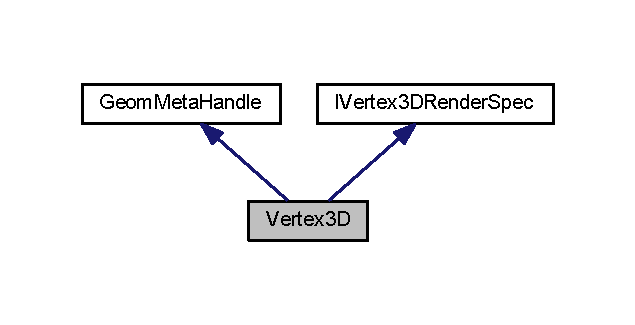
\includegraphics[width=305pt]{class_vertex3_d__inherit__graph}
\end{center}
\end{figure}


Collaboration diagram for Vertex3\-D\-:\nopagebreak
\begin{figure}[H]
\begin{center}
\leavevmode
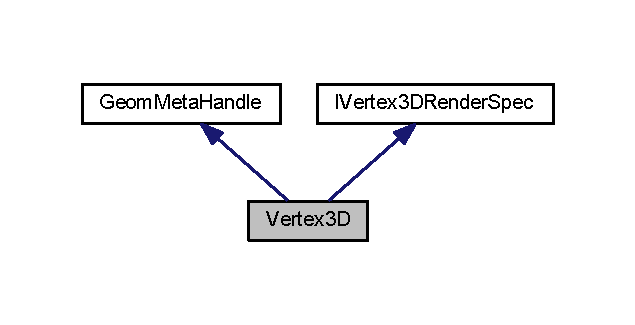
\includegraphics[width=305pt]{class_vertex3_d__coll__graph}
\end{center}
\end{figure}
\subsection*{Public Member Functions}
\begin{DoxyCompactItemize}
\item 
\hypertarget{class_vertex3_d_a41dee42f7502bdc4b04be44a4bf4bdbc}{\hyperlink{class_vertex3_d_a41dee42f7502bdc4b04be44a4bf4bdbc}{Vertex3\-D} ()}\label{class_vertex3_d_a41dee42f7502bdc4b04be44a4bf4bdbc}

\begin{DoxyCompactList}\small\item\em Constructor. Initialises position and I\-D to zero. \end{DoxyCompactList}\item 
\hyperlink{class_vertex3_d_a81b68cf7e781884ed457034bd5b63612}{Vertex3\-D} (const float x, const float y, const float z)
\begin{DoxyCompactList}\small\item\em Constructor specifying vertex position. \end{DoxyCompactList}\item 
\hyperlink{class_vertex3_d_a11ea685931b50972afb2ffda7bfaa984}{Vertex3\-D} (const Q\-Vector3\-D vec)
\begin{DoxyCompactList}\small\item\em Constructor specifying vertex position. \end{DoxyCompactList}\item 
Q\-Vector3\-D \hyperlink{class_vertex3_d_aefb3922097ae3d982370671c2c83fe1d}{get\-Position} () const 
\begin{DoxyCompactList}\small\item\em Gets the vertex's position local to its parent geometry object. \end{DoxyCompactList}\item 
Q\-Color \hyperlink{class_vertex3_d_a2bdd677bf1eb764a7dfa967aa7d2660b}{get\-Colour} () const 
\begin{DoxyCompactList}\small\item\em Gets the vertex's render colour. \end{DoxyCompactList}\item 
Q\-Vector3\-D \hyperlink{class_vertex3_d_a02604a70c43c9ef567684174e8406959}{get\-Normal} () const 
\begin{DoxyCompactList}\small\item\em Gets this vertex's normal. \end{DoxyCompactList}\item 
float \hyperlink{class_vertex3_d_ad22bd676ad371c1a3ba6e987e0704733}{get\-Tex\-Coord\-X} () const 
\begin{DoxyCompactList}\small\item\em Gets this vertex's X texture co-\/ordinate. \end{DoxyCompactList}\item 
float \hyperlink{class_vertex3_d_a3b6eab91dea0d4eb0c53d6c414bda232}{get\-Tex\-Coord\-Y} () const 
\begin{DoxyCompactList}\small\item\em Gets this vertex's Y texture co-\/ordinate. \end{DoxyCompactList}\item 
\hyperlink{vertex_8h_a2e2e1374aac5842116c8683f3b06e99f}{V\-B\-O\-\_\-\-O\-F\-F\-S\-E\-T} \hyperlink{class_vertex3_d_a04dca81ead78614468f7028913a2a582}{get\-V\-B\-O\-Offset} () const 
\begin{DoxyCompactList}\small\item\em Gets this vertex's V\-B\-O offset from the beginning of the parent solid. This offset it not valid if the parent solid is N\-U\-L\-L\-H\-N\-D. \end{DoxyCompactList}\item 
\hyperlink{vertex_8h_a72202e57358ed73cd212e9a2eaf39aeb}{G\-E\-O\-M\-H\-A\-N\-D\-L\-E} \hyperlink{class_vertex3_d_a77b0e7b96b5ec626d56ea32963111c37}{get\-Parent\-Solid} () const 
\begin{DoxyCompactList}\small\item\em Gets the handle of this vertex's parent solid. \end{DoxyCompactList}\item 
\hyperlink{vertex_8h_a72202e57358ed73cd212e9a2eaf39aeb}{G\-E\-O\-M\-H\-A\-N\-D\-L\-E} \hyperlink{class_vertex3_d_acd4bdbddebb5090650cd31883280175e}{get\-Handle} () const 
\begin{DoxyCompactList}\small\item\em Returns this vertex's handle, which is unique within its parent solid. \end{DoxyCompactList}\item 
void \hyperlink{class_vertex3_d_a0727071117d99f6a5f5227b54d41a7cf}{set\-Position} (const float x, const float y, const float z)
\begin{DoxyCompactList}\small\item\em Sets the vertex's position. \end{DoxyCompactList}\item 
void \hyperlink{class_vertex3_d_a62274f5655891dc5dfe979bc2c57ded6}{set\-Position} (const Q\-Vector3\-D pos)
\begin{DoxyCompactList}\small\item\em Sets the vertex's position. \end{DoxyCompactList}\item 
void \hyperlink{class_vertex3_d_ac922ca7c683657d60be4147d17d2d74e}{set\-Colour} (const Q\-Color colour)
\begin{DoxyCompactList}\small\item\em Sets the vertex's render colour. \end{DoxyCompactList}\item 
void \hyperlink{class_vertex3_d_a512576966b5a70493353df7f3571e727}{set\-Normal} (const Q\-Vector3\-D normal)
\begin{DoxyCompactList}\small\item\em Sets this vertex's normal. \end{DoxyCompactList}\item 
void \hyperlink{class_vertex3_d_a8fba559b69d9ba907d962c7154321854}{set\-Tex\-Coord\-X} (const float coord)
\begin{DoxyCompactList}\small\item\em Sets this vertex's X texture co-\/ordinate. \end{DoxyCompactList}\item 
void \hyperlink{class_vertex3_d_a72cc82c3b015c4aabd5a2223933655b5}{set\-Tex\-Coord\-Y} (const float coord)
\begin{DoxyCompactList}\small\item\em Sets this vertex's Y texture co-\/ordinate. \end{DoxyCompactList}\item 
void \hyperlink{class_vertex3_d_a8201535f83d869bb1421e7d36962624a}{set\-V\-B\-O\-Offset} (const \hyperlink{vertex_8h_a2e2e1374aac5842116c8683f3b06e99f}{V\-B\-O\-\_\-\-O\-F\-F\-S\-E\-T} offset)
\begin{DoxyCompactList}\small\item\em Sets this vertex's V\-B\-O offset. \end{DoxyCompactList}\item 
void \hyperlink{class_vertex3_d_aec0f45cdc6b03ec560fd4c352c6bd694}{set\-Parent\-Solid} (const \hyperlink{vertex_8h_a72202e57358ed73cd212e9a2eaf39aeb}{G\-E\-O\-M\-H\-A\-N\-D\-L\-E} handle)
\begin{DoxyCompactList}\small\item\em Sets this vertex's parent solid handle. \end{DoxyCompactList}\item 
void \hyperlink{class_vertex3_d_a53670951cc49d1b5ae9d03d08a11d581}{set\-Handle} (const \hyperlink{vertex_8h_a72202e57358ed73cd212e9a2eaf39aeb}{G\-E\-O\-M\-H\-A\-N\-D\-L\-E} handle)
\begin{DoxyCompactList}\small\item\em Sets this vertex's handle. \end{DoxyCompactList}\item 
virtual void \hyperlink{class_vertex3_d_a1d95bf448d6cf90c2ba78ab22167b806}{V3\-R\-S\-\_\-\-Position} (float position\mbox{[}$\,$\mbox{]})
\begin{DoxyCompactList}\small\item\em Fills an array with the position values for this vertex. \end{DoxyCompactList}\item 
virtual void \hyperlink{class_vertex3_d_a40126d514f76cfef6ebf2855380338e1}{V3\-R\-S\-\_\-\-Colour} (unsigned char colour\mbox{[}$\,$\mbox{]})
\begin{DoxyCompactList}\small\item\em Fills an array with the colour values for this vertex. \end{DoxyCompactList}\item 
virtual void \hyperlink{class_vertex3_d_aea2d1d899ec54fc166fd04baeee64a91}{V3\-R\-S\-\_\-\-Texture\-\_\-\-Coords} (float coords\mbox{[}$\,$\mbox{]})
\begin{DoxyCompactList}\small\item\em Fills an array with the texture co-\/ordinate values for this vertex. \end{DoxyCompactList}\item 
virtual unsigned long \hyperlink{class_vertex3_d_a13a922fd8180591636c1daf4687cc205}{V3\-R\-S\-\_\-\-Offset} ()
\begin{DoxyCompactList}\small\item\em Returns the offset of this vertex from the beginning of the V\-B\-O, in V3\-R\-S\-\_\-\-T\-O\-T\-A\-L\-\_\-\-D\-A\-T\-A\-\_\-\-T\-R\-A\-N\-S\-F\-E\-R strides. \end{DoxyCompactList}\end{DoxyCompactItemize}
\subsection*{Additional Inherited Members}


\subsection{Detailed Description}
Defines a vertex in 3\-D space. 

The vertex contains a V\-B\-O offset which, when combined with the parent solid's offset, defines where in the V\-B\-O this vertex's render data is found. The vertex also contains colour information and texture co-\/ordinates. Normals are not stored per vertex as when faces are rendered, the face's stored normal is used to calculate the shading required. 

\subsection{Constructor \& Destructor Documentation}
\hypertarget{class_vertex3_d_a81b68cf7e781884ed457034bd5b63612}{\index{Vertex3\-D@{Vertex3\-D}!Vertex3\-D@{Vertex3\-D}}
\index{Vertex3\-D@{Vertex3\-D}!Vertex3D@{Vertex3\-D}}
\subsubsection[{Vertex3\-D}]{\setlength{\rightskip}{0pt plus 5cm}Vertex3\-D\-::\-Vertex3\-D (
\begin{DoxyParamCaption}
\item[{const float}]{x, }
\item[{const float}]{y, }
\item[{const float}]{z}
\end{DoxyParamCaption}
)\hspace{0.3cm}{\ttfamily [inline]}}}\label{class_vertex3_d_a81b68cf7e781884ed457034bd5b63612}


Constructor specifying vertex position. 


\begin{DoxyParams}{Parameters}
{\em x} & X position. \\
\hline
{\em y} & Y position. \\
\hline
{\em z} & Z position. \\
\hline
\end{DoxyParams}
\hypertarget{class_vertex3_d_a11ea685931b50972afb2ffda7bfaa984}{\index{Vertex3\-D@{Vertex3\-D}!Vertex3\-D@{Vertex3\-D}}
\index{Vertex3\-D@{Vertex3\-D}!Vertex3D@{Vertex3\-D}}
\subsubsection[{Vertex3\-D}]{\setlength{\rightskip}{0pt plus 5cm}Vertex3\-D\-::\-Vertex3\-D (
\begin{DoxyParamCaption}
\item[{const Q\-Vector3\-D}]{vec}
\end{DoxyParamCaption}
)\hspace{0.3cm}{\ttfamily [inline]}}}\label{class_vertex3_d_a11ea685931b50972afb2ffda7bfaa984}


Constructor specifying vertex position. 


\begin{DoxyParams}{Parameters}
{\em vec} & Vector representing position. \\
\hline
\end{DoxyParams}


\subsection{Member Function Documentation}
\hypertarget{class_vertex3_d_a2bdd677bf1eb764a7dfa967aa7d2660b}{\index{Vertex3\-D@{Vertex3\-D}!get\-Colour@{get\-Colour}}
\index{get\-Colour@{get\-Colour}!Vertex3D@{Vertex3\-D}}
\subsubsection[{get\-Colour}]{\setlength{\rightskip}{0pt plus 5cm}Q\-Color Vertex3\-D\-::get\-Colour (
\begin{DoxyParamCaption}
{}
\end{DoxyParamCaption}
) const\hspace{0.3cm}{\ttfamily [inline]}}}\label{class_vertex3_d_a2bdd677bf1eb764a7dfa967aa7d2660b}


Gets the vertex's render colour. 

\begin{DoxyReturn}{Returns}
Render colour. 
\end{DoxyReturn}
\hypertarget{class_vertex3_d_acd4bdbddebb5090650cd31883280175e}{\index{Vertex3\-D@{Vertex3\-D}!get\-Handle@{get\-Handle}}
\index{get\-Handle@{get\-Handle}!Vertex3D@{Vertex3\-D}}
\subsubsection[{get\-Handle}]{\setlength{\rightskip}{0pt plus 5cm}{\bf G\-E\-O\-M\-H\-A\-N\-D\-L\-E} Vertex3\-D\-::get\-Handle (
\begin{DoxyParamCaption}
{}
\end{DoxyParamCaption}
) const\hspace{0.3cm}{\ttfamily [inline]}}}\label{class_vertex3_d_acd4bdbddebb5090650cd31883280175e}


Returns this vertex's handle, which is unique within its parent solid. 

\begin{DoxyReturn}{Returns}
This vertex's handle. 
\end{DoxyReturn}
\hypertarget{class_vertex3_d_a02604a70c43c9ef567684174e8406959}{\index{Vertex3\-D@{Vertex3\-D}!get\-Normal@{get\-Normal}}
\index{get\-Normal@{get\-Normal}!Vertex3D@{Vertex3\-D}}
\subsubsection[{get\-Normal}]{\setlength{\rightskip}{0pt plus 5cm}Q\-Vector3\-D Vertex3\-D\-::get\-Normal (
\begin{DoxyParamCaption}
{}
\end{DoxyParamCaption}
) const\hspace{0.3cm}{\ttfamily [inline]}}}\label{class_vertex3_d_a02604a70c43c9ef567684174e8406959}


Gets this vertex's normal. 

\begin{DoxyReturn}{Returns}
Normal vector. 
\end{DoxyReturn}
\hypertarget{class_vertex3_d_a77b0e7b96b5ec626d56ea32963111c37}{\index{Vertex3\-D@{Vertex3\-D}!get\-Parent\-Solid@{get\-Parent\-Solid}}
\index{get\-Parent\-Solid@{get\-Parent\-Solid}!Vertex3D@{Vertex3\-D}}
\subsubsection[{get\-Parent\-Solid}]{\setlength{\rightskip}{0pt plus 5cm}{\bf G\-E\-O\-M\-H\-A\-N\-D\-L\-E} Vertex3\-D\-::get\-Parent\-Solid (
\begin{DoxyParamCaption}
{}
\end{DoxyParamCaption}
) const\hspace{0.3cm}{\ttfamily [inline]}}}\label{class_vertex3_d_a77b0e7b96b5ec626d56ea32963111c37}


Gets the handle of this vertex's parent solid. 

\begin{DoxyReturn}{Returns}
Parent solid's handle, or N\-U\-L\-L\-H\-N\-D if no parent solid exists. 
\end{DoxyReturn}
\hypertarget{class_vertex3_d_aefb3922097ae3d982370671c2c83fe1d}{\index{Vertex3\-D@{Vertex3\-D}!get\-Position@{get\-Position}}
\index{get\-Position@{get\-Position}!Vertex3D@{Vertex3\-D}}
\subsubsection[{get\-Position}]{\setlength{\rightskip}{0pt plus 5cm}Q\-Vector3\-D Vertex3\-D\-::get\-Position (
\begin{DoxyParamCaption}
{}
\end{DoxyParamCaption}
) const\hspace{0.3cm}{\ttfamily [inline]}}}\label{class_vertex3_d_aefb3922097ae3d982370671c2c83fe1d}


Gets the vertex's position local to its parent geometry object. 

\begin{DoxyReturn}{Returns}
Vector representing position. 
\end{DoxyReturn}
\hypertarget{class_vertex3_d_ad22bd676ad371c1a3ba6e987e0704733}{\index{Vertex3\-D@{Vertex3\-D}!get\-Tex\-Coord\-X@{get\-Tex\-Coord\-X}}
\index{get\-Tex\-Coord\-X@{get\-Tex\-Coord\-X}!Vertex3D@{Vertex3\-D}}
\subsubsection[{get\-Tex\-Coord\-X}]{\setlength{\rightskip}{0pt plus 5cm}float Vertex3\-D\-::get\-Tex\-Coord\-X (
\begin{DoxyParamCaption}
{}
\end{DoxyParamCaption}
) const\hspace{0.3cm}{\ttfamily [inline]}}}\label{class_vertex3_d_ad22bd676ad371c1a3ba6e987e0704733}


Gets this vertex's X texture co-\/ordinate. 

\begin{DoxyReturn}{Returns}
X co-\/ordinate. 
\end{DoxyReturn}
\hypertarget{class_vertex3_d_a3b6eab91dea0d4eb0c53d6c414bda232}{\index{Vertex3\-D@{Vertex3\-D}!get\-Tex\-Coord\-Y@{get\-Tex\-Coord\-Y}}
\index{get\-Tex\-Coord\-Y@{get\-Tex\-Coord\-Y}!Vertex3D@{Vertex3\-D}}
\subsubsection[{get\-Tex\-Coord\-Y}]{\setlength{\rightskip}{0pt plus 5cm}float Vertex3\-D\-::get\-Tex\-Coord\-Y (
\begin{DoxyParamCaption}
{}
\end{DoxyParamCaption}
) const\hspace{0.3cm}{\ttfamily [inline]}}}\label{class_vertex3_d_a3b6eab91dea0d4eb0c53d6c414bda232}


Gets this vertex's Y texture co-\/ordinate. 

\begin{DoxyReturn}{Returns}
Y co-\/ordinate. 
\end{DoxyReturn}
\hypertarget{class_vertex3_d_a04dca81ead78614468f7028913a2a582}{\index{Vertex3\-D@{Vertex3\-D}!get\-V\-B\-O\-Offset@{get\-V\-B\-O\-Offset}}
\index{get\-V\-B\-O\-Offset@{get\-V\-B\-O\-Offset}!Vertex3D@{Vertex3\-D}}
\subsubsection[{get\-V\-B\-O\-Offset}]{\setlength{\rightskip}{0pt plus 5cm}{\bf V\-B\-O\-\_\-\-O\-F\-F\-S\-E\-T} Vertex3\-D\-::get\-V\-B\-O\-Offset (
\begin{DoxyParamCaption}
{}
\end{DoxyParamCaption}
) const\hspace{0.3cm}{\ttfamily [inline]}}}\label{class_vertex3_d_a04dca81ead78614468f7028913a2a582}


Gets this vertex's V\-B\-O offset from the beginning of the parent solid. This offset it not valid if the parent solid is N\-U\-L\-L\-H\-N\-D. 

\begin{DoxyReturn}{Returns}
Vertex's V\-B\-O offset. 
\end{DoxyReturn}
\hypertarget{class_vertex3_d_ac922ca7c683657d60be4147d17d2d74e}{\index{Vertex3\-D@{Vertex3\-D}!set\-Colour@{set\-Colour}}
\index{set\-Colour@{set\-Colour}!Vertex3D@{Vertex3\-D}}
\subsubsection[{set\-Colour}]{\setlength{\rightskip}{0pt plus 5cm}void Vertex3\-D\-::set\-Colour (
\begin{DoxyParamCaption}
\item[{const Q\-Color}]{colour}
\end{DoxyParamCaption}
)\hspace{0.3cm}{\ttfamily [inline]}}}\label{class_vertex3_d_ac922ca7c683657d60be4147d17d2d74e}


Sets the vertex's render colour. 


\begin{DoxyParams}{Parameters}
{\em colour} & Colour to set. \\
\hline
\end{DoxyParams}
\hypertarget{class_vertex3_d_a53670951cc49d1b5ae9d03d08a11d581}{\index{Vertex3\-D@{Vertex3\-D}!set\-Handle@{set\-Handle}}
\index{set\-Handle@{set\-Handle}!Vertex3D@{Vertex3\-D}}
\subsubsection[{set\-Handle}]{\setlength{\rightskip}{0pt plus 5cm}void Vertex3\-D\-::set\-Handle (
\begin{DoxyParamCaption}
\item[{const {\bf G\-E\-O\-M\-H\-A\-N\-D\-L\-E}}]{handle}
\end{DoxyParamCaption}
)\hspace{0.3cm}{\ttfamily [inline]}}}\label{class_vertex3_d_a53670951cc49d1b5ae9d03d08a11d581}


Sets this vertex's handle. 


\begin{DoxyParams}{Parameters}
{\em handle} & Handle to set. \\
\hline
\end{DoxyParams}
\hypertarget{class_vertex3_d_a512576966b5a70493353df7f3571e727}{\index{Vertex3\-D@{Vertex3\-D}!set\-Normal@{set\-Normal}}
\index{set\-Normal@{set\-Normal}!Vertex3D@{Vertex3\-D}}
\subsubsection[{set\-Normal}]{\setlength{\rightskip}{0pt plus 5cm}void Vertex3\-D\-::set\-Normal (
\begin{DoxyParamCaption}
\item[{const Q\-Vector3\-D}]{normal}
\end{DoxyParamCaption}
)\hspace{0.3cm}{\ttfamily [inline]}}}\label{class_vertex3_d_a512576966b5a70493353df7f3571e727}


Sets this vertex's normal. 


\begin{DoxyParams}{Parameters}
{\em normal} & Normal to set. \\
\hline
\end{DoxyParams}
\hypertarget{class_vertex3_d_aec0f45cdc6b03ec560fd4c352c6bd694}{\index{Vertex3\-D@{Vertex3\-D}!set\-Parent\-Solid@{set\-Parent\-Solid}}
\index{set\-Parent\-Solid@{set\-Parent\-Solid}!Vertex3D@{Vertex3\-D}}
\subsubsection[{set\-Parent\-Solid}]{\setlength{\rightskip}{0pt plus 5cm}void Vertex3\-D\-::set\-Parent\-Solid (
\begin{DoxyParamCaption}
\item[{const {\bf G\-E\-O\-M\-H\-A\-N\-D\-L\-E}}]{handle}
\end{DoxyParamCaption}
)\hspace{0.3cm}{\ttfamily [inline]}}}\label{class_vertex3_d_aec0f45cdc6b03ec560fd4c352c6bd694}


Sets this vertex's parent solid handle. 


\begin{DoxyParams}{Parameters}
{\em handle} & Handle to set. \\
\hline
\end{DoxyParams}
\hypertarget{class_vertex3_d_a0727071117d99f6a5f5227b54d41a7cf}{\index{Vertex3\-D@{Vertex3\-D}!set\-Position@{set\-Position}}
\index{set\-Position@{set\-Position}!Vertex3D@{Vertex3\-D}}
\subsubsection[{set\-Position}]{\setlength{\rightskip}{0pt plus 5cm}void Vertex3\-D\-::set\-Position (
\begin{DoxyParamCaption}
\item[{const float}]{x, }
\item[{const float}]{y, }
\item[{const float}]{z}
\end{DoxyParamCaption}
)\hspace{0.3cm}{\ttfamily [inline]}}}\label{class_vertex3_d_a0727071117d99f6a5f5227b54d41a7cf}


Sets the vertex's position. 


\begin{DoxyParams}{Parameters}
{\em x} & X position. \\
\hline
{\em y} & Y position. \\
\hline
{\em z} & Z position. \\
\hline
\end{DoxyParams}
\hypertarget{class_vertex3_d_a62274f5655891dc5dfe979bc2c57ded6}{\index{Vertex3\-D@{Vertex3\-D}!set\-Position@{set\-Position}}
\index{set\-Position@{set\-Position}!Vertex3D@{Vertex3\-D}}
\subsubsection[{set\-Position}]{\setlength{\rightskip}{0pt plus 5cm}void Vertex3\-D\-::set\-Position (
\begin{DoxyParamCaption}
\item[{const Q\-Vector3\-D}]{pos}
\end{DoxyParamCaption}
)\hspace{0.3cm}{\ttfamily [inline]}}}\label{class_vertex3_d_a62274f5655891dc5dfe979bc2c57ded6}


Sets the vertex's position. 


\begin{DoxyParams}{Parameters}
{\em pos} & Vector representing position. \\
\hline
\end{DoxyParams}
\hypertarget{class_vertex3_d_a8fba559b69d9ba907d962c7154321854}{\index{Vertex3\-D@{Vertex3\-D}!set\-Tex\-Coord\-X@{set\-Tex\-Coord\-X}}
\index{set\-Tex\-Coord\-X@{set\-Tex\-Coord\-X}!Vertex3D@{Vertex3\-D}}
\subsubsection[{set\-Tex\-Coord\-X}]{\setlength{\rightskip}{0pt plus 5cm}void Vertex3\-D\-::set\-Tex\-Coord\-X (
\begin{DoxyParamCaption}
\item[{const float}]{coord}
\end{DoxyParamCaption}
)\hspace{0.3cm}{\ttfamily [inline]}}}\label{class_vertex3_d_a8fba559b69d9ba907d962c7154321854}


Sets this vertex's X texture co-\/ordinate. 


\begin{DoxyParams}{Parameters}
{\em coord} & Co-\/ord to set. \\
\hline
\end{DoxyParams}
\hypertarget{class_vertex3_d_a72cc82c3b015c4aabd5a2223933655b5}{\index{Vertex3\-D@{Vertex3\-D}!set\-Tex\-Coord\-Y@{set\-Tex\-Coord\-Y}}
\index{set\-Tex\-Coord\-Y@{set\-Tex\-Coord\-Y}!Vertex3D@{Vertex3\-D}}
\subsubsection[{set\-Tex\-Coord\-Y}]{\setlength{\rightskip}{0pt plus 5cm}void Vertex3\-D\-::set\-Tex\-Coord\-Y (
\begin{DoxyParamCaption}
\item[{const float}]{coord}
\end{DoxyParamCaption}
)\hspace{0.3cm}{\ttfamily [inline]}}}\label{class_vertex3_d_a72cc82c3b015c4aabd5a2223933655b5}


Sets this vertex's Y texture co-\/ordinate. 


\begin{DoxyParams}{Parameters}
{\em coord} & Co-\/ord to set. \\
\hline
\end{DoxyParams}
\hypertarget{class_vertex3_d_a8201535f83d869bb1421e7d36962624a}{\index{Vertex3\-D@{Vertex3\-D}!set\-V\-B\-O\-Offset@{set\-V\-B\-O\-Offset}}
\index{set\-V\-B\-O\-Offset@{set\-V\-B\-O\-Offset}!Vertex3D@{Vertex3\-D}}
\subsubsection[{set\-V\-B\-O\-Offset}]{\setlength{\rightskip}{0pt plus 5cm}void Vertex3\-D\-::set\-V\-B\-O\-Offset (
\begin{DoxyParamCaption}
\item[{const {\bf V\-B\-O\-\_\-\-O\-F\-F\-S\-E\-T}}]{offset}
\end{DoxyParamCaption}
)\hspace{0.3cm}{\ttfamily [inline]}}}\label{class_vertex3_d_a8201535f83d869bb1421e7d36962624a}


Sets this vertex's V\-B\-O offset. 


\begin{DoxyParams}{Parameters}
{\em offset} & Offset to set. \\
\hline
\end{DoxyParams}
\hypertarget{class_vertex3_d_a40126d514f76cfef6ebf2855380338e1}{\index{Vertex3\-D@{Vertex3\-D}!V3\-R\-S\-\_\-\-Colour@{V3\-R\-S\-\_\-\-Colour}}
\index{V3\-R\-S\-\_\-\-Colour@{V3\-R\-S\-\_\-\-Colour}!Vertex3D@{Vertex3\-D}}
\subsubsection[{V3\-R\-S\-\_\-\-Colour}]{\setlength{\rightskip}{0pt plus 5cm}virtual void Vertex3\-D\-::\-V3\-R\-S\-\_\-\-Colour (
\begin{DoxyParamCaption}
\item[{unsigned char}]{colour\mbox{[}$\,$\mbox{]}}
\end{DoxyParamCaption}
)\hspace{0.3cm}{\ttfamily [inline]}, {\ttfamily [virtual]}}}\label{class_vertex3_d_a40126d514f76cfef6ebf2855380338e1}


Fills an array with the colour values for this vertex. 


\begin{DoxyParams}{Parameters}
{\em colour} & Colour values. Format is R\-G\-B\-A, range 0.\-0 -\/ 1.\-0. \\
\hline
\end{DoxyParams}
\hypertarget{class_vertex3_d_a13a922fd8180591636c1daf4687cc205}{\index{Vertex3\-D@{Vertex3\-D}!V3\-R\-S\-\_\-\-Offset@{V3\-R\-S\-\_\-\-Offset}}
\index{V3\-R\-S\-\_\-\-Offset@{V3\-R\-S\-\_\-\-Offset}!Vertex3D@{Vertex3\-D}}
\subsubsection[{V3\-R\-S\-\_\-\-Offset}]{\setlength{\rightskip}{0pt plus 5cm}virtual unsigned long Vertex3\-D\-::\-V3\-R\-S\-\_\-\-Offset (
\begin{DoxyParamCaption}
{}
\end{DoxyParamCaption}
)\hspace{0.3cm}{\ttfamily [inline]}, {\ttfamily [virtual]}}}\label{class_vertex3_d_a13a922fd8180591636c1daf4687cc205}


Returns the offset of this vertex from the beginning of the V\-B\-O, in V3\-R\-S\-\_\-\-T\-O\-T\-A\-L\-\_\-\-D\-A\-T\-A\-\_\-\-T\-R\-A\-N\-S\-F\-E\-R strides. 

\begin{DoxyReturn}{Returns}
Offset for this vertex. 
\end{DoxyReturn}


Implements \hyperlink{class_i_vertex3_d_render_spec_a891d736d3d414de333398975f34bbae7}{I\-Vertex3\-D\-Render\-Spec}.

\hypertarget{class_vertex3_d_a1d95bf448d6cf90c2ba78ab22167b806}{\index{Vertex3\-D@{Vertex3\-D}!V3\-R\-S\-\_\-\-Position@{V3\-R\-S\-\_\-\-Position}}
\index{V3\-R\-S\-\_\-\-Position@{V3\-R\-S\-\_\-\-Position}!Vertex3D@{Vertex3\-D}}
\subsubsection[{V3\-R\-S\-\_\-\-Position}]{\setlength{\rightskip}{0pt plus 5cm}virtual void Vertex3\-D\-::\-V3\-R\-S\-\_\-\-Position (
\begin{DoxyParamCaption}
\item[{float}]{position\mbox{[}$\,$\mbox{]}}
\end{DoxyParamCaption}
)\hspace{0.3cm}{\ttfamily [inline]}, {\ttfamily [virtual]}}}\label{class_vertex3_d_a1d95bf448d6cf90c2ba78ab22167b806}


Fills an array with the position values for this vertex. 


\begin{DoxyParams}{Parameters}
{\em position} & Array to fill. Format is X\-Y\-Z. \\
\hline
\end{DoxyParams}
\hypertarget{class_vertex3_d_aea2d1d899ec54fc166fd04baeee64a91}{\index{Vertex3\-D@{Vertex3\-D}!V3\-R\-S\-\_\-\-Texture\-\_\-\-Coords@{V3\-R\-S\-\_\-\-Texture\-\_\-\-Coords}}
\index{V3\-R\-S\-\_\-\-Texture\-\_\-\-Coords@{V3\-R\-S\-\_\-\-Texture\-\_\-\-Coords}!Vertex3D@{Vertex3\-D}}
\subsubsection[{V3\-R\-S\-\_\-\-Texture\-\_\-\-Coords}]{\setlength{\rightskip}{0pt plus 5cm}virtual void Vertex3\-D\-::\-V3\-R\-S\-\_\-\-Texture\-\_\-\-Coords (
\begin{DoxyParamCaption}
\item[{float}]{coords\mbox{[}$\,$\mbox{]}}
\end{DoxyParamCaption}
)\hspace{0.3cm}{\ttfamily [inline]}, {\ttfamily [virtual]}}}\label{class_vertex3_d_aea2d1d899ec54fc166fd04baeee64a91}


Fills an array with the texture co-\/ordinate values for this vertex. 


\begin{DoxyParams}{Parameters}
{\em coords} & Array to fill. Format is X\-Y. \\
\hline
\end{DoxyParams}


The documentation for this class was generated from the following file\-:\begin{DoxyCompactItemize}
\item 
app/\hyperlink{vertex_8h}{vertex.\-h}\end{DoxyCompactItemize}

\chapter{File Documentation}
\hypertarget{commandlineparser_8h}{\section{app/commandlineparser.h File Reference}
\label{commandlineparser_8h}\index{app/commandlineparser.\-h@{app/commandlineparser.\-h}}
}


Defines the class responsible for parsing command-\/line arguments and setting the relevant settings in response.  


{\ttfamily \#include $<$Q\-Object$>$}\\*
Include dependency graph for commandlineparser.\-h\-:
\nopagebreak
\begin{figure}[H]
\begin{center}
\leavevmode
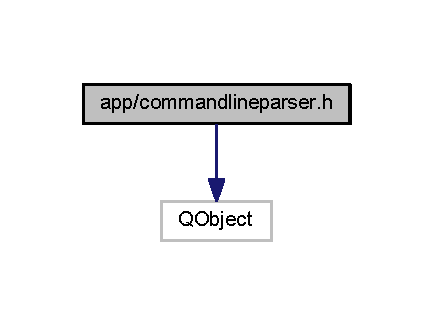
\includegraphics[width=208pt]{commandlineparser_8h__incl}
\end{center}
\end{figure}
\subsection*{Classes}
\begin{DoxyCompactItemize}
\item 
class \hyperlink{class_command_line_parser}{Command\-Line\-Parser}
\begin{DoxyCompactList}\small\item\em Deals with arguments passed to the application on the command-\/line. \end{DoxyCompactList}\end{DoxyCompactItemize}
\subsection*{Macros}
\begin{DoxyCompactItemize}
\item 
\hypertarget{commandlineparser_8h_a28d598b46f4ac21d6aef06c46089f3cb}{\#define \hyperlink{commandlineparser_8h_a28d598b46f4ac21d6aef06c46089f3cb}{C\-L\-A\-\_\-\-D\-E\-B\-U\-G\-G\-I\-N\-G}~\char`\"{}-\/debug\char`\"{}}\label{commandlineparser_8h_a28d598b46f4ac21d6aef06c46089f3cb}

\begin{DoxyCompactList}\small\item\em Command-\/line option string to enable debugging. \end{DoxyCompactList}\item 
\hypertarget{commandlineparser_8h_a886e3ba324ee7244ccb5c79dd2d1cddb}{\#define \hyperlink{commandlineparser_8h_a886e3ba324ee7244ccb5c79dd2d1cddb}{C\-L\-A\-\_\-\-L\-O\-G\-G\-I\-N\-G}~\char`\"{}-\/log\char`\"{}}\label{commandlineparser_8h_a886e3ba324ee7244ccb5c79dd2d1cddb}

\begin{DoxyCompactList}\small\item\em Command-\/line option string to enable logging. \end{DoxyCompactList}\end{DoxyCompactItemize}


\subsection{Detailed Description}
Defines the class responsible for parsing command-\/line arguments and setting the relevant settings in response. 
\hypertarget{consolewindow_8h}{\section{app/consolewindow.h File Reference}
\label{consolewindow_8h}\index{app/consolewindow.\-h@{app/consolewindow.\-h}}
}


Defines the \hyperlink{class_console_window}{Console\-Window} class for showing a developer console.  


{\ttfamily \#include $<$Q\-Widget$>$}\\*
{\ttfamily \#include \char`\"{}commandsenderinfo.\-h\char`\"{}}\\*
Include dependency graph for consolewindow.\-h\-:\nopagebreak
\begin{figure}[H]
\begin{center}
\leavevmode
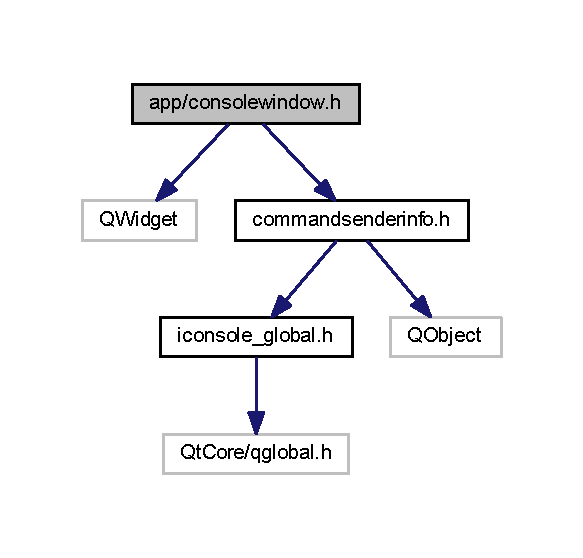
\includegraphics[width=280pt]{consolewindow_8h__incl}
\end{center}
\end{figure}
\subsection*{Classes}
\begin{DoxyCompactItemize}
\item 
class \hyperlink{class_console_window}{Console\-Window}
\begin{DoxyCompactList}\small\item\em Ties together the main elements from the I\-Console library to create a functioning console window. \end{DoxyCompactList}\end{DoxyCompactItemize}


\subsection{Detailed Description}
Defines the \hyperlink{class_console_window}{Console\-Window} class for showing a developer console. 
\hypertarget{edge_8h}{\section{app/edge.h File Reference}
\label{edge_8h}\index{app/edge.\-h@{app/edge.\-h}}
}


Defines an edge which links two vertices.  


{\ttfamily \#include \char`\"{}vertex.\-h\char`\"{}}\\*
Include dependency graph for edge.\-h\-:\nopagebreak
\begin{figure}[H]
\begin{center}
\leavevmode
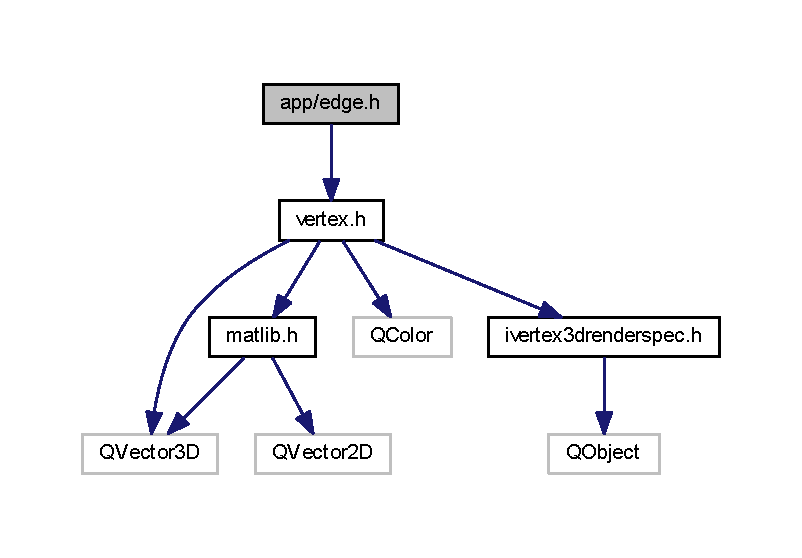
\includegraphics[width=350pt]{edge_8h__incl}
\end{center}
\end{figure}
This graph shows which files directly or indirectly include this file\-:\nopagebreak
\begin{figure}[H]
\begin{center}
\leavevmode
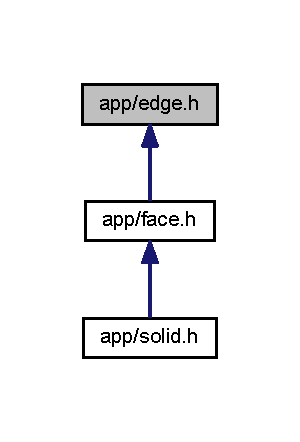
\includegraphics[width=144pt]{edge_8h__dep__incl}
\end{center}
\end{figure}
\subsection*{Classes}
\begin{DoxyCompactItemize}
\item 
class \hyperlink{class_edge3_d}{Edge3\-D}
\begin{DoxyCompactList}\small\item\em An edge links two vertices and two faces, referenced by their geometry handles.\par
 When considering travelling along the edge from the beginning to end vertex, the normals of the faces either side of the edge can be considered to point clockwise or anticlockwise around the edge. The face with an anticlockwise-\/pointing normal is denoted the \char`\"{}right\char`\"{} face (if the normal were pointing upwards the face would be positioned to the right of the edge) and the face with the clockwise-\/pointing normal is denoted the \char`\"{}left\char`\"{} face. If both normals are pointing in the same direction (either clockwise or anticlockwise) it is not defined which face is denoted left and which right. \end{DoxyCompactList}\end{DoxyCompactItemize}


\subsection{Detailed Description}
Defines an edge which links two vertices. 
\hypertarget{face_8h}{\section{app/face.h File Reference}
\label{face_8h}\index{app/face.\-h@{app/face.\-h}}
}


Defines a 3\-D face. Solids are built up of these faces. Faces reference edges, which in turn reference vertices.  


{\ttfamily \#include \char`\"{}edge.\-h\char`\"{}}\\*
{\ttfamily \#include $<$Q\-List$>$}\\*
{\ttfamily \#include \char`\"{}plane.\-h\char`\"{}}\\*
Include dependency graph for face.\-h\-:\nopagebreak
\begin{figure}[H]
\begin{center}
\leavevmode
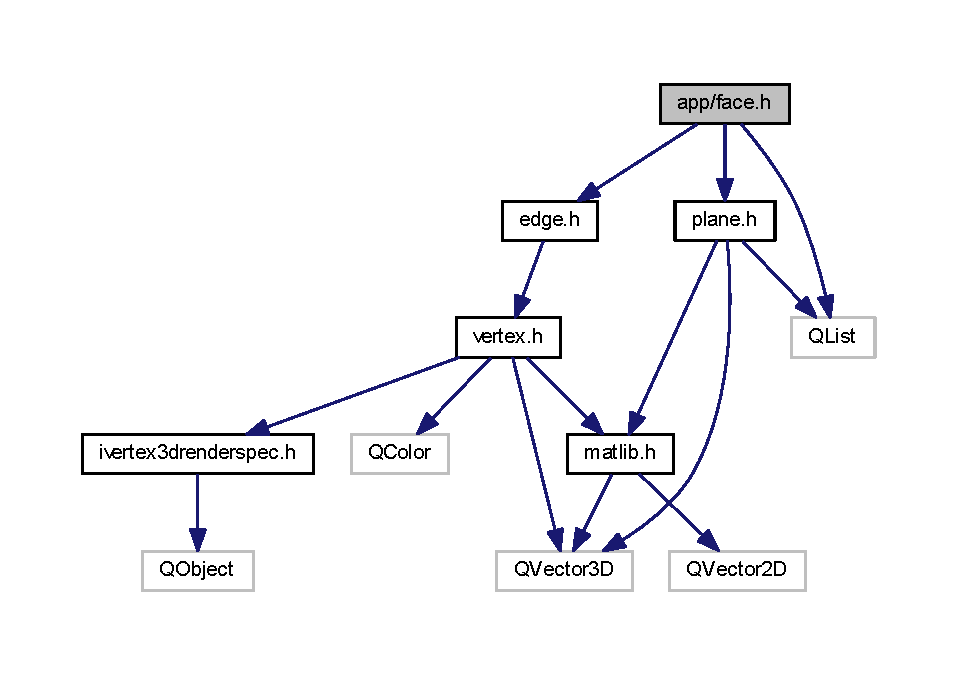
\includegraphics[width=350pt]{face_8h__incl}
\end{center}
\end{figure}
This graph shows which files directly or indirectly include this file\-:\nopagebreak
\begin{figure}[H]
\begin{center}
\leavevmode
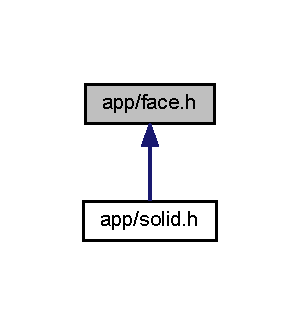
\includegraphics[width=144pt]{face_8h__dep__incl}
\end{center}
\end{figure}
\subsection*{Classes}
\begin{DoxyCompactItemize}
\item 
class \hyperlink{class_face3_d}{Face3\-D}
\begin{DoxyCompactList}\small\item\em Class representing a 3\-D face. \end{DoxyCompactList}\end{DoxyCompactItemize}


\subsection{Detailed Description}
Defines a 3\-D face. Solids are built up of these faces. Faces reference edges, which in turn reference vertices. 
\hypertarget{globals_8h}{\section{app/globals.h File Reference}
\label{globals_8h}\index{app/globals.\-h@{app/globals.\-h}}
}


Defines global variables and classes.  


{\ttfamily \#include $<$Q\-List$>$}\\*
{\ttfamily \#include \char`\"{}commandsenderinfo.\-h\char`\"{}}\\*
Include dependency graph for globals.\-h\-:\nopagebreak
\begin{figure}[H]
\begin{center}
\leavevmode
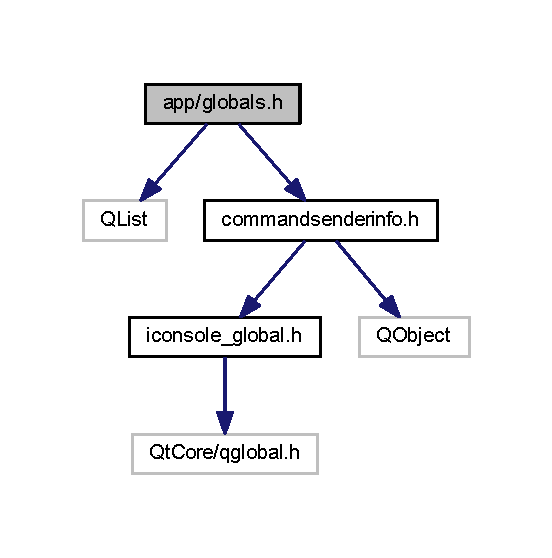
\includegraphics[width=265pt]{globals_8h__incl}
\end{center}
\end{figure}
\subsection*{Macros}
\begin{DoxyCompactItemize}
\item 
\#define \hyperlink{group___global_variables_gaf9c6d8de2e7b3d11f070bb500d62edce}{D\-E\-F\-I\-N\-E\-\_\-\-C\-O\-N\-V\-A\-R}(sz\-Name\-\_\-\-No\-Quote, sz\-Def\-Val, p\-Callback, sz\-Desc, i\-Flags, b\-Min, fl\-Min, b\-Max, fl\-Max)~\hyperlink{class_con_var}{Con\-Var} sz\-Name\-\_\-\-No\-Quote(\#sz\-Name\-\_\-\-No\-Quote, sz\-Def\-Val, \hyperlink{group___global_variables_ga4d39defaa5d22f29bde4c75d590bd0fe}{g\-\_\-p\-Command\-Manager}, \&\hyperlink{group___global_variables_ga8389c826239a1bc627ae3b7f97a79fe4}{g\-\_\-p\-Command\-List}, p\-Callback, sz\-Desc, i\-Flags, b\-Min, fl\-Min, b\-Max, fl\-Max);
\begin{DoxyCompactList}\small\item\em Macro for defining a \hyperlink{class_con_var}{Con\-Var} with the default command manager and list. \end{DoxyCompactList}\item 
\#define \hyperlink{group___global_variables_ga5c65583f94cc62a481b1846c0e6e3344}{D\-E\-F\-I\-N\-E\-\_\-\-C\-O\-N\-C\-O\-M\-M\-A\-N\-D}(sz\-Name\-\_\-\-No\-Quote, p\-Callback, sz\-Desc, i\-Flags)~\hyperlink{class_con_command}{Con\-Command} sz\-Name\-\_\-\-No\-Quote(\#sz\-Name\-\_\-\-No\-Quote, p\-Callback, \hyperlink{group___global_variables_ga4d39defaa5d22f29bde4c75d590bd0fe}{g\-\_\-p\-Command\-Manager}, \&\hyperlink{group___global_variables_ga8389c826239a1bc627ae3b7f97a79fe4}{g\-\_\-p\-Command\-List}, sz\-Desc, i\-Flags);
\begin{DoxyCompactList}\small\item\em Macro for defining a \hyperlink{class_con_command}{Con\-Command} with the default command manager and list. \end{DoxyCompactList}\end{DoxyCompactItemize}
\subsection*{Functions}
\begin{DoxyCompactItemize}
\item 
void \hyperlink{group___global_variables_ga9551f73a6927861d0b6f5d7901c90888}{Show\-Message\-Box} (Q\-String message)
\begin{DoxyCompactList}\small\item\em Creates a basic one-\/time modal message box with simple message and an \char`\"{}\-O\-K\char`\"{} button. \end{DoxyCompactList}\item 
void \hyperlink{group___global_variables_gadf8a13f3d23660f424828d7f559addd3}{Show\-Error\-Box} (Q\-String message)
\begin{DoxyCompactList}\small\item\em Creates a basic one-\/time modal error box with simple message and an \char`\"{}\-O\-K\char`\"{} button. \end{DoxyCompactList}\item 
void \hyperlink{group___global_variables_ga1788dc69b89b298a038015cbb83f8183}{Log\-Message} (const Q\-String \&message, bool newline=true)
\begin{DoxyCompactList}\small\item\em Logs a message to the log window. \end{DoxyCompactList}\item 
void \hyperlink{group___global_variables_gacb9fa8876388ad9319c61d9ae4d21510}{Log\-Tagged\-Message} (const Q\-String \&tag, const Q\-String \&message, bool newline=true)
\begin{DoxyCompactList}\small\item\em Logs a tagged message. \end{DoxyCompactList}\item 
void \hyperlink{group___global_variables_ga4b2863ab23932e06f2b5f292c66e7ef6}{Log\-Warning} (const Q\-String \&message, bool newline=true)
\begin{DoxyCompactList}\small\item\em Logs a warning to the log window. Log text is printed red and in bold. \end{DoxyCompactList}\item 
void \hyperlink{group___global_variables_ga49e471be032d9340fe6b4c251d1aef21}{Log\-Tagged\-Warning} (const Q\-String \&tag, const Q\-String \&message, bool newline=true)
\begin{DoxyCompactList}\small\item\em Logs a tagged warning to the log window. Log text is printed red and in bold. \end{DoxyCompactList}\item 
void \hyperlink{group___global_variables_gab9e5c16962c3cdcd7220de6dfa5a70b5}{Log\-Output} (\hyperlink{class_command_sender_info_a3a5e6a2ef1772f6557f351652c2e3b60}{Command\-Sender\-Info\-::\-Output\-Type} type, const Q\-String \&message, bool newline=true)
\begin{DoxyCompactList}\small\item\em Logs output of the specified type to the log window. \end{DoxyCompactList}\item 
void \hyperlink{group___global_variables_ga63348a368c397865f05d9a17c94752c6}{Log\-Tagged\-Output} (\hyperlink{class_command_sender_info_a3a5e6a2ef1772f6557f351652c2e3b60}{Command\-Sender\-Info\-::\-Output\-Type} type, const Q\-String \&tag, const Q\-String \&message, bool newline=true)
\begin{DoxyCompactList}\small\item\em Logs tagged output of the specified type to the log window. \end{DoxyCompactList}\end{DoxyCompactItemize}
\subsection*{Variables}
\begin{DoxyCompactItemize}
\item 
\hyperlink{class_command_line_parser}{Command\-Line\-Parser} $\ast$ \hyperlink{group___global_variables_ga270fc6d9322b018e011978d6376f43ba}{g\-\_\-p\-Cmd\-Line}
\begin{DoxyCompactList}\small\item\em Global command-\/line parser object. \end{DoxyCompactList}\item 
\hyperlink{class_console_window}{Console\-Window} $\ast$ \hyperlink{group___global_variables_gae2d76408535137add345d6e4258c5a07}{g\-\_\-p\-Log}
\begin{DoxyCompactList}\small\item\em Global console window object. \end{DoxyCompactList}\item 
Q\-List$<$ \hyperlink{class_main_win}{Main\-Win} $\ast$ $>$ $\ast$ \hyperlink{group___global_variables_gab5d481b5087f9956e533067ad8001d78}{g\-\_\-p\-Window\-Tracker}
\begin{DoxyCompactList}\small\item\em Global window tracker object. \end{DoxyCompactList}\item 
\hyperlink{class_listed_command_manager}{Listed\-Command\-Manager} $\ast$ \hyperlink{group___global_variables_ga4d39defaa5d22f29bde4c75d590bd0fe}{g\-\_\-p\-Command\-Manager}
\begin{DoxyCompactList}\small\item\em Global console command manager, created in main.\-cpp. \end{DoxyCompactList}\item 
\hypertarget{group___global_variables_ga347a4723fad5c3711958f787dfc93fa4}{\hyperlink{class_command_interpreter}{Command\-Interpreter} $\ast$ \hyperlink{group___global_variables_ga347a4723fad5c3711958f787dfc93fa4}{g\-\_\-p\-Command\-Interpreter}}\label{group___global_variables_ga347a4723fad5c3711958f787dfc93fa4}

\begin{DoxyCompactList}\small\item\em Global console command interpreter, created in main.\-cpp. \end{DoxyCompactList}\item 
\hyperlink{class_listed_console_command}{Listed\-Console\-Command} $\ast$ \hyperlink{group___global_variables_ga8389c826239a1bc627ae3b7f97a79fe4}{g\-\_\-p\-Command\-List}
\begin{DoxyCompactList}\small\item\em Global console command list pointer. \end{DoxyCompactList}\end{DoxyCompactItemize}


\subsection{Detailed Description}
Defines global variables and classes. This file defines certain classes and variables which should be visible from anywhere in the application. Examples include the command-\/line parser, the log window and the window tracker. Some classes or properties have convenience macros defined. 
\hypertarget{indexpool_8h}{\section{app/indexpool.h File Reference}
\label{indexpool_8h}\index{app/indexpool.\-h@{app/indexpool.\-h}}
}


Defines the \hyperlink{class_index_pool}{Index\-Pool} class which manages non-\/consecutive array indices.  


{\ttfamily \#include $<$Q\-Object$>$}\\*
{\ttfamily \#include $<$Q\-Map$>$}\\*
{\ttfamily \#include \char`\"{}vertex.\-h\char`\"{}}\\*
Include dependency graph for indexpool.\-h\-:\nopagebreak
\begin{figure}[H]
\begin{center}
\leavevmode
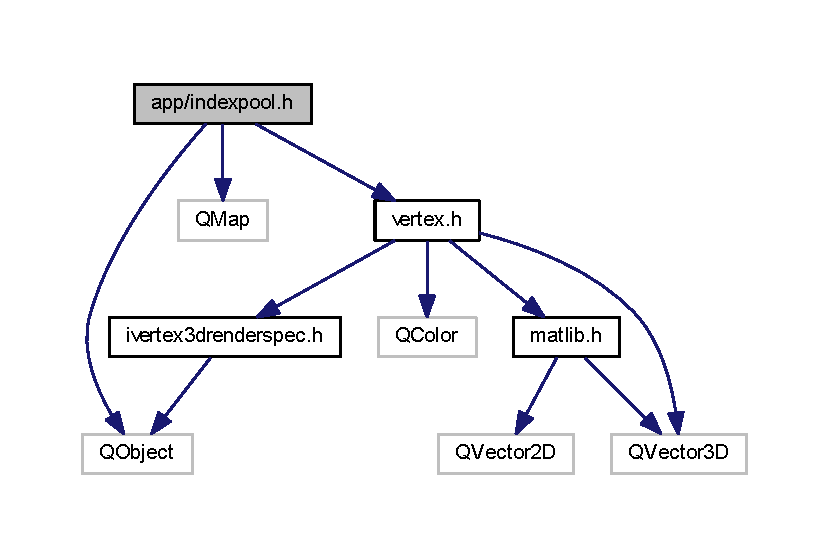
\includegraphics[width=350pt]{indexpool_8h__incl}
\end{center}
\end{figure}
This graph shows which files directly or indirectly include this file\-:\nopagebreak
\begin{figure}[H]
\begin{center}
\leavevmode
\includegraphics[width=164pt]{indexpool_8h__dep__incl}
\end{center}
\end{figure}
\subsection*{Classes}
\begin{DoxyCompactItemize}
\item 
class \hyperlink{class_index_pool}{Index\-Pool}
\begin{DoxyCompactList}\small\item\em The \hyperlink{class_index_pool}{Index\-Pool} class manages non-\/consecutive array indices. \end{DoxyCompactList}\end{DoxyCompactItemize}


\subsection{Detailed Description}
Defines the \hyperlink{class_index_pool}{Index\-Pool} class which manages non-\/consecutive array indices. 
\hypertarget{ivertex3drenderspec_8h}{\section{app/ivertex3drenderspec.h File Reference}
\label{ivertex3drenderspec_8h}\index{app/ivertex3drenderspec.\-h@{app/ivertex3drenderspec.\-h}}
}


Defines the interface between map vertices and the vertices used for rendering.  


{\ttfamily \#include $<$Q\-Object$>$}\\*
Include dependency graph for ivertex3drenderspec.\-h\-:\nopagebreak
\begin{figure}[H]
\begin{center}
\leavevmode
\includegraphics[width=210pt]{ivertex3drenderspec_8h__incl}
\end{center}
\end{figure}
This graph shows which files directly or indirectly include this file\-:\nopagebreak
\begin{figure}[H]
\begin{center}
\leavevmode
\includegraphics[width=245pt]{ivertex3drenderspec_8h__dep__incl}
\end{center}
\end{figure}
\subsection*{Classes}
\begin{DoxyCompactItemize}
\item 
class \hyperlink{class_i_vertex3_d_render_spec}{I\-Vertex3\-D\-Render\-Spec}
\begin{DoxyCompactList}\small\item\em Defines the properties required to be exposed by renderable vertices. \end{DoxyCompactList}\end{DoxyCompactItemize}
\subsection*{Macros}
\begin{DoxyCompactItemize}
\item 
\hypertarget{ivertex3drenderspec_8h_afd14dd1ec641943da1c3cd81a0037c0d}{\#define \hyperlink{ivertex3drenderspec_8h_afd14dd1ec641943da1c3cd81a0037c0d}{I\-Vertex3\-D\-Render\-Spec\-\_\-iid}~\char`\"{}Crowbar.\-Interfaces.\-I\-Vertex3\-D\-Render\-Spec\char`\"{}}\label{ivertex3drenderspec_8h_afd14dd1ec641943da1c3cd81a0037c0d}

\begin{DoxyCompactList}\small\item\em Unique I\-D for \hyperlink{class_i_vertex3_d_render_spec}{I\-Vertex3\-D\-Render\-Spec} interface. \end{DoxyCompactList}\end{DoxyCompactItemize}


\subsection{Detailed Description}
Defines the interface between map vertices and the vertices used for rendering. This file describes the requirements for a map vertex in terms of what information is required by the rendering engine. In order for a vertex to be rendered, it must implement these functions. 
\hypertarget{mainwin_8h}{\section{app/mainwin.h File Reference}
\label{mainwin_8h}\index{app/mainwin.\-h@{app/mainwin.\-h}}
}


Defines a main application window corresponding to one currently open map document.  


{\ttfamily \#include $<$Q\-Main\-Window$>$}\\*
{\ttfamily \#include $<$Q\-Application$>$}\\*
{\ttfamily \#include $<$Q\-Close\-Event$>$}\\*
Include dependency graph for mainwin.\-h\-:\nopagebreak
\begin{figure}[H]
\begin{center}
\leavevmode
\includegraphics[width=341pt]{mainwin_8h__incl}
\end{center}
\end{figure}
\subsection*{Classes}
\begin{DoxyCompactItemize}
\item 
class \hyperlink{class_main_win}{Main\-Win}
\begin{DoxyCompactList}\small\item\em Application window class. \end{DoxyCompactList}\end{DoxyCompactItemize}


\subsection{Detailed Description}
Defines a main application window corresponding to one currently open map document. 
\hypertarget{mapdoc_8h}{\section{app/mapdoc.h File Reference}
\label{mapdoc_8h}\index{app/mapdoc.\-h@{app/mapdoc.\-h}}
}


The main map document class.  


{\ttfamily \#include $<$Q\-Object$>$}\\*
{\ttfamily \#include \char`\"{}octree/octree.\-h\char`\"{}}\\*
Include dependency graph for mapdoc.\-h\-:
\nopagebreak
\begin{figure}[H]
\begin{center}
\leavevmode
\includegraphics[width=233pt]{mapdoc_8h__incl}
\end{center}
\end{figure}
\subsection*{Classes}
\begin{DoxyCompactItemize}
\item 
class \hyperlink{class_map_doc}{Map\-Doc}
\begin{DoxyCompactList}\small\item\em The \hyperlink{class_map_doc}{Map\-Doc} class. \end{DoxyCompactList}\end{DoxyCompactItemize}
\subsection*{Macros}
\begin{DoxyCompactItemize}
\item 
\hypertarget{mapdoc_8h_af6699d6ffa298734e45b6a64604eb0ab}{\#define \hyperlink{mapdoc_8h_af6699d6ffa298734e45b6a64604eb0ab}{M\-A\-P\-D\-O\-C\-\_\-\-V\-E\-R\-S\-I\-O\-N}~10}\label{mapdoc_8h_af6699d6ffa298734e45b6a64604eb0ab}

\begin{DoxyCompactList}\small\item\em Current version of the mapdoc\-: \mbox{[}major\mbox{]}\mbox{[}minor\mbox{]}. \end{DoxyCompactList}\end{DoxyCompactItemize}


\subsection{Detailed Description}
The main map document class. The \hyperlink{class_map_doc}{Map\-Doc} class details any information that will be serialised when a map source file is saved. This includes geometry and entities but also settings such as camera positions, grid size, snapping, etc. Geometry and entities are kept inside an octree that represents the entire 3\-D space in the level.

\begin{DoxyNote}{Note}
Simon Perreault's octree's documentation can be found at \href{http://nomis80.org/code/doc/classOctree.html}{\tt http\-://nomis80.\-org/code/doc/class\-Octree.\-html} 
\end{DoxyNote}

\hypertarget{matlib_8h}{\section{app/matlib.h File Reference}
\label{matlib_8h}\index{app/matlib.\-h@{app/matlib.\-h}}
}


Contains convenient custom maths functions.  


{\ttfamily \#include $<$Q\-Vector3\-D$>$}\\*
{\ttfamily \#include $<$Q\-Vector2\-D$>$}\\*
Include dependency graph for matlib.\-h\-:
\nopagebreak
\begin{figure}[H]
\begin{center}
\leavevmode
\includegraphics[width=227pt]{matlib_8h__incl}
\end{center}
\end{figure}
This graph shows which files directly or indirectly include this file\-:
\nopagebreak
\begin{figure}[H]
\begin{center}
\leavevmode
\includegraphics[width=300pt]{matlib_8h__dep__incl}
\end{center}
\end{figure}
\subsection*{Functions}
\begin{DoxyCompactItemize}
\item 
\hypertarget{matlib_8h_abbca97a4f576c9ea1a52b3ab4fe9a483}{static const Q\-Vector2\-D \hyperlink{matlib_8h_abbca97a4f576c9ea1a52b3ab4fe9a483}{V\-E\-C2\-\_\-\-O\-R\-I\-G\-I\-N} (0.\-0, 0.\-0)}\label{matlib_8h_abbca97a4f576c9ea1a52b3ab4fe9a483}

\begin{DoxyCompactList}\small\item\em Null 2\-D vector\-: (0.\-0, 0.\-0). \end{DoxyCompactList}\item 
\hypertarget{matlib_8h_ac2de4dab97258eff87e0a1253a2d1a29}{static const Q\-Vector3\-D \hyperlink{matlib_8h_ac2de4dab97258eff87e0a1253a2d1a29}{V\-E\-C3\-\_\-\-O\-R\-I\-G\-I\-N} (0.\-0, 0.\-0, 0.\-0)}\label{matlib_8h_ac2de4dab97258eff87e0a1253a2d1a29}

\begin{DoxyCompactList}\small\item\em Null 3\-D vector\-: (0.\-0, 0.\-0, 0.\-0). \end{DoxyCompactList}\end{DoxyCompactItemize}


\subsection{Detailed Description}
Contains convenient custom maths functions. 
\hypertarget{plane_8h}{\section{app/plane.h File Reference}
\label{plane_8h}\index{app/plane.\-h@{app/plane.\-h}}
}


Defines a plane class to hold the co-\/ordinates of a plane in 3\-D space.  


{\ttfamily \#include \char`\"{}matlib.\-h\char`\"{}}\\*
{\ttfamily \#include $<$Q\-Vector3\-D$>$}\\*
{\ttfamily \#include $<$Q\-List$>$}\\*
Include dependency graph for plane.\-h\-:
\nopagebreak
\begin{figure}[H]
\begin{center}
\leavevmode
\includegraphics[width=250pt]{plane_8h__incl}
\end{center}
\end{figure}
This graph shows which files directly or indirectly include this file\-:
\nopagebreak
\begin{figure}[H]
\begin{center}
\leavevmode
\includegraphics[width=146pt]{plane_8h__dep__incl}
\end{center}
\end{figure}
\subsection*{Classes}
\begin{DoxyCompactItemize}
\item 
class \hyperlink{class_plane}{Plane}
\begin{DoxyCompactList}\small\item\em Defines a plane in 3\-D space. \end{DoxyCompactList}\end{DoxyCompactItemize}


\subsection{Detailed Description}
Defines a plane class to hold the co-\/ordinates of a plane in 3\-D space. The plane class contains three points that define the plane and a normal that defines its front. Planes can be invalid, which means that two or more of their defining points are identical. 
\hypertarget{solid_8h}{\section{app/solid.h File Reference}
\label{solid_8h}\index{app/solid.\-h@{app/solid.\-h}}
}


Defines a solid class.  


{\ttfamily \#include $<$Q\-Vector$>$}\\*
{\ttfamily \#include \char`\"{}face.\-h\char`\"{}}\\*
{\ttfamily \#include \char`\"{}indexpool.\-h\char`\"{}}\\*
Include dependency graph for solid.\-h\-:
\nopagebreak
\begin{figure}[H]
\begin{center}
\leavevmode
\includegraphics[width=350pt]{solid_8h__incl}
\end{center}
\end{figure}
\subsection*{Classes}
\begin{DoxyCompactItemize}
\item 
struct \hyperlink{struct_geom_info}{Geom\-Info}
\begin{DoxyCompactList}\small\item\em Struct to hold and pass information about geometry objects. \end{DoxyCompactList}\item 
class \hyperlink{class_solid3_d}{Solid3\-D}
\begin{DoxyCompactList}\small\item\em Class representing a 3\-D solid. \end{DoxyCompactList}\end{DoxyCompactItemize}


\subsection{Detailed Description}
Defines a solid class. Solids are the programmatical implementation of brushes and are made up of sets of vertices, edges and faces. Each edge references the vertices it links, and each face is built from multiple edges. As opposed to Hammer's implementation, solids are mesh-\/based (ie. they are defined by vertex positions and links rather than planes and intersections) to allow for easier manipulation, and are exported as plane-\/based objects when serialised as a V\-M\-F.\par
 It is recommended to work {\bfseries bottom-\/up} (ie. add any required vertices before edges, and edges before faces) rather than {\bfseries top-\/down} (creating all of a face's edges and vertices as the face itself is created) as the former method is less prone to errors. 
\hypertarget{vertex_8h}{\section{app/vertex.h File Reference}
\label{vertex_8h}\index{app/vertex.\-h@{app/vertex.\-h}}
}


T\-O\-D\-O.  


{\ttfamily \#include \char`\"{}matlib.\-h\char`\"{}}\\*
{\ttfamily \#include $<$Q\-Vector3\-D$>$}\\*
{\ttfamily \#include $<$Q\-Color$>$}\\*
{\ttfamily \#include \char`\"{}ivertex3drenderspec.\-h\char`\"{}}\\*
Include dependency graph for vertex.\-h\-:
\nopagebreak
\begin{figure}[H]
\begin{center}
\leavevmode
\includegraphics[width=350pt]{vertex_8h__incl}
\end{center}
\end{figure}
This graph shows which files directly or indirectly include this file\-:
\nopagebreak
\begin{figure}[H]
\begin{center}
\leavevmode
\includegraphics[width=245pt]{vertex_8h__dep__incl}
\end{center}
\end{figure}
\subsection*{Classes}
\begin{DoxyCompactItemize}
\item 
class \hyperlink{class_geom_meta_handle}{Geom\-Meta\-Handle}
\begin{DoxyCompactList}\small\item\em Metaclass which all geometry components subclass from. Contains useful metadata relevant to geometry components. \end{DoxyCompactList}\item 
class \hyperlink{class_vertex3_d}{Vertex3\-D}
\begin{DoxyCompactList}\small\item\em Defines a vertex in 3\-D space. \end{DoxyCompactList}\end{DoxyCompactItemize}
\subsection*{Macros}
\begin{DoxyCompactItemize}
\item 
\hypertarget{vertex_8h_a58600f71cdacd3fb41515de8749fe861}{\#define \hyperlink{vertex_8h_a58600f71cdacd3fb41515de8749fe861}{N\-U\-L\-L\-H\-N\-D}~0}\label{vertex_8h_a58600f71cdacd3fb41515de8749fe861}

\begin{DoxyCompactList}\small\item\em Value of a null G\-E\-O\-M\-H\-A\-N\-D\-L\-E. \end{DoxyCompactList}\end{DoxyCompactItemize}
\subsection*{Typedefs}
\begin{DoxyCompactItemize}
\item 
\hypertarget{vertex_8h_a72202e57358ed73cd212e9a2eaf39aeb}{typedef unsigned long \hyperlink{vertex_8h_a72202e57358ed73cd212e9a2eaf39aeb}{G\-E\-O\-M\-H\-A\-N\-D\-L\-E}}\label{vertex_8h_a72202e57358ed73cd212e9a2eaf39aeb}

\begin{DoxyCompactList}\small\item\em Handle for a geometry component. \end{DoxyCompactList}\item 
\hypertarget{vertex_8h_a2e2e1374aac5842116c8683f3b06e99f}{typedef unsigned long \hyperlink{vertex_8h_a2e2e1374aac5842116c8683f3b06e99f}{V\-B\-O\-\_\-\-O\-F\-F\-S\-E\-T}}\label{vertex_8h_a2e2e1374aac5842116c8683f3b06e99f}

\begin{DoxyCompactList}\small\item\em Value for specifying an offset in the graphics V\-B\-O. \end{DoxyCompactList}\end{DoxyCompactItemize}


\subsection{Detailed Description}
T\-O\-D\-O. 
\hypertarget{baseconsolecommand_8h}{\section{I\-Console/inc/baseconsolecommand.h File Reference}
\label{baseconsolecommand_8h}\index{I\-Console/inc/baseconsolecommand.\-h@{I\-Console/inc/baseconsolecommand.\-h}}
}


Describes the base properties common to all console commands and variables.  


{\ttfamily \#include \char`\"{}iconsole\-\_\-global.\-h\char`\"{}}\\*
{\ttfamily \#include $<$Q\-Object$>$}\\*
{\ttfamily \#include $<$Q\-List$>$}\\*
{\ttfamily \#include $<$Q\-String$>$}\\*
{\ttfamily \#include \char`\"{}nglobalcmd.\-h\char`\"{}}\\*
Include dependency graph for baseconsolecommand.\-h\-:\nopagebreak
\begin{figure}[H]
\begin{center}
\leavevmode
\includegraphics[width=350pt]{baseconsolecommand_8h__incl}
\end{center}
\end{figure}
This graph shows which files directly or indirectly include this file\-:\nopagebreak
\begin{figure}[H]
\begin{center}
\leavevmode
\includegraphics[width=350pt]{baseconsolecommand_8h__dep__incl}
\end{center}
\end{figure}
\subsection*{Classes}
\begin{DoxyCompactItemize}
\item 
class \hyperlink{class_base_console_command}{Base\-Console\-Command}
\begin{DoxyCompactList}\small\item\em Class defining properties common to all console commands. \end{DoxyCompactList}\end{DoxyCompactItemize}


\subsection{Detailed Description}
Describes the base properties common to all console commands and variables. 
\hypertarget{commandentrybox_8h}{\section{I\-Console/inc/commandentrybox.h File Reference}
\label{commandentrybox_8h}\index{I\-Console/inc/commandentrybox.\-h@{I\-Console/inc/commandentrybox.\-h}}
}


Defines the \hyperlink{class_command_entry_box}{Command\-Entry\-Box} class which manages the input of console commands by the user.  


{\ttfamily \#include $<$Q\-Line\-Edit$>$}\\*
{\ttfamily \#include $<$Q\-List$>$}\\*
{\ttfamily \#include \char`\"{}iconsole\-\_\-global.\-h\char`\"{}}\\*
{\ttfamily \#include \char`\"{}commandinterpreter.\-h\char`\"{}}\\*
Include dependency graph for commandentrybox.\-h\-:\nopagebreak
\begin{figure}[H]
\begin{center}
\leavevmode
\includegraphics[width=350pt]{commandentrybox_8h__incl}
\end{center}
\end{figure}
This graph shows which files directly or indirectly include this file\-:\nopagebreak
\begin{figure}[H]
\begin{center}
\leavevmode
\includegraphics[width=256pt]{commandentrybox_8h__dep__incl}
\end{center}
\end{figure}
\subsection*{Classes}
\begin{DoxyCompactItemize}
\item 
class \hyperlink{class_command_entry_box}{Command\-Entry\-Box}
\begin{DoxyCompactList}\small\item\em Manages input of console commands by the user. \end{DoxyCompactList}\end{DoxyCompactItemize}


\subsection{Detailed Description}
Defines the \hyperlink{class_command_entry_box}{Command\-Entry\-Box} class which manages the input of console commands by the user. 
\hypertarget{commandinterpreter_8h}{\section{I\-Console/inc/commandinterpreter.h File Reference}
\label{commandinterpreter_8h}\index{I\-Console/inc/commandinterpreter.\-h@{I\-Console/inc/commandinterpreter.\-h}}
}


Defines the \hyperlink{class_command_interpreter}{Command\-Interpreter} class to interpret raw user-\/input command strings.  


{\ttfamily \#include \char`\"{}iconsole\-\_\-global.\-h\char`\"{}}\\*
{\ttfamily \#include \char`\"{}nglobalcmd.\-h\char`\"{}}\\*
{\ttfamily \#include $<$Q\-Object$>$}\\*
{\ttfamily \#include $<$Q\-String$>$}\\*
{\ttfamily \#include $<$Q\-List$>$}\\*
{\ttfamily \#include $<$Q\-Pair$>$}\\*
{\ttfamily \#include $<$Q\-Regular\-Expression$>$}\\*
Include dependency graph for commandinterpreter.\-h\-:\nopagebreak
\begin{figure}[H]
\begin{center}
\leavevmode
\includegraphics[width=350pt]{commandinterpreter_8h__incl}
\end{center}
\end{figure}
This graph shows which files directly or indirectly include this file\-:\nopagebreak
\begin{figure}[H]
\begin{center}
\leavevmode
\includegraphics[width=350pt]{commandinterpreter_8h__dep__incl}
\end{center}
\end{figure}
\subsection*{Classes}
\begin{DoxyCompactItemize}
\item 
class \hyperlink{class_command_interpreter}{Command\-Interpreter}
\begin{DoxyCompactList}\small\item\em Handles parsing strings of user input and executing the relevant commands. \end{DoxyCompactList}\end{DoxyCompactItemize}


\subsection{Detailed Description}
Defines the \hyperlink{class_command_interpreter}{Command\-Interpreter} class to interpret raw user-\/input command strings. 
\hypertarget{commandmanager_8h}{\section{I\-Console/inc/commandmanager.h File Reference}
\label{commandmanager_8h}\index{I\-Console/inc/commandmanager.\-h@{I\-Console/inc/commandmanager.\-h}}
}


Defines the \hyperlink{class_command_manager}{Command\-Manager} class which allows quick searching for a console command or variable by name.  


{\ttfamily \#include \char`\"{}iconsole\-\_\-global.\-h\char`\"{}}\\*
{\ttfamily \#include $<$Q\-Object$>$}\\*
{\ttfamily \#include $<$Q\-String$>$}\\*
{\ttfamily \#include $<$Q\-Regular\-Expression$>$}\\*
{\ttfamily \#include \char`\"{}nglobalcmd.\-h\char`\"{}}\\*
{\ttfamily \#include \char`\"{}commandsenderinfo.\-h\char`\"{}}\\*
Include dependency graph for commandmanager.\-h\-:\nopagebreak
\begin{figure}[H]
\begin{center}
\leavevmode
\includegraphics[width=350pt]{commandmanager_8h__incl}
\end{center}
\end{figure}
This graph shows which files directly or indirectly include this file\-:\nopagebreak
\begin{figure}[H]
\begin{center}
\leavevmode
\includegraphics[width=350pt]{commandmanager_8h__dep__incl}
\end{center}
\end{figure}
\subsection*{Classes}
\begin{DoxyCompactItemize}
\item 
class \hyperlink{class_command_manager}{Command\-Manager}
\begin{DoxyCompactList}\small\item\em Allows quick searching for console commands and variables by their name. \end{DoxyCompactList}\end{DoxyCompactItemize}


\subsection{Detailed Description}
Defines the \hyperlink{class_command_manager}{Command\-Manager} class which allows quick searching for a console command or variable by name. 
\hypertarget{commandsenderinfo_8h}{\section{I\-Console/inc/commandsenderinfo.h File Reference}
\label{commandsenderinfo_8h}\index{I\-Console/inc/commandsenderinfo.\-h@{I\-Console/inc/commandsenderinfo.\-h}}
}
{\ttfamily \#include \char`\"{}iconsole\-\_\-global.\-h\char`\"{}}\\*
{\ttfamily \#include $<$Q\-Object$>$}\\*
Include dependency graph for commandsenderinfo.\-h\-:\nopagebreak
\begin{figure}[H]
\begin{center}
\leavevmode
\includegraphics[width=255pt]{commandsenderinfo_8h__incl}
\end{center}
\end{figure}
This graph shows which files directly or indirectly include this file\-:\nopagebreak
\begin{figure}[H]
\begin{center}
\leavevmode
\includegraphics[width=350pt]{commandsenderinfo_8h__dep__incl}
\end{center}
\end{figure}
\subsection*{Classes}
\begin{DoxyCompactItemize}
\item 
class \hyperlink{class_command_sender_info}{Command\-Sender\-Info}
\begin{DoxyCompactList}\small\item\em The \hyperlink{class_command_sender_info}{Command\-Sender\-Info} class provides a route between a calling \hyperlink{class_command_manager}{Command\-Manager} and a receiving \hyperlink{class_con_command}{Con\-Command} or \hyperlink{class_con_var}{Con\-Var}. The command or variable can print output to the relevant console window (if one exists) by passing the output to this class. \end{DoxyCompactList}\end{DoxyCompactItemize}

\hypertarget{commandsuggestionlist_8h}{\section{I\-Console/inc/commandsuggestionlist.h File Reference}
\label{commandsuggestionlist_8h}\index{I\-Console/inc/commandsuggestionlist.\-h@{I\-Console/inc/commandsuggestionlist.\-h}}
}


Defines the \hyperlink{class_command_suggestion_list}{Command\-Suggestion\-List} class which holds suggestions for the currently typed command.  


{\ttfamily \#include \char`\"{}iconsole\-\_\-global.\-h\char`\"{}}\\*
{\ttfamily \#include $<$Q\-List\-Widget$>$}\\*
Include dependency graph for commandsuggestionlist.\-h\-:\nopagebreak
\begin{figure}[H]
\begin{center}
\leavevmode
\includegraphics[width=268pt]{commandsuggestionlist_8h__incl}
\end{center}
\end{figure}
This graph shows which files directly or indirectly include this file\-:\nopagebreak
\begin{figure}[H]
\begin{center}
\leavevmode
\includegraphics[width=264pt]{commandsuggestionlist_8h__dep__incl}
\end{center}
\end{figure}
\subsection*{Classes}
\begin{DoxyCompactItemize}
\item 
class \hyperlink{class_command_suggestion_list}{Command\-Suggestion\-List}
\begin{DoxyCompactList}\small\item\em Holds and displays console command suggestions to the user. \end{DoxyCompactList}\end{DoxyCompactItemize}


\subsection{Detailed Description}
Defines the \hyperlink{class_command_suggestion_list}{Command\-Suggestion\-List} class which holds suggestions for the currently typed command. 
\hypertarget{concommand_8h}{\section{I\-Console/inc/concommand.h File Reference}
\label{concommand_8h}\index{I\-Console/inc/concommand.\-h@{I\-Console/inc/concommand.\-h}}
}


Defines the \hyperlink{class_con_command}{Con\-Command} class, for executing code from the console.  


{\ttfamily \#include \char`\"{}iconsole\-\_\-global.\-h\char`\"{}}\\*
{\ttfamily \#include $<$Q\-String$>$}\\*
{\ttfamily \#include $<$Q\-List$>$}\\*
{\ttfamily \#include $<$Q\-Variant$>$}\\*
{\ttfamily \#include \char`\"{}nglobalcmd.\-h\char`\"{}}\\*
{\ttfamily \#include \char`\"{}listedconsolecommand.\-h\char`\"{}}\\*
Include dependency graph for concommand.\-h\-:\nopagebreak
\begin{figure}[H]
\begin{center}
\leavevmode
\includegraphics[width=350pt]{concommand_8h__incl}
\end{center}
\end{figure}
This graph shows which files directly or indirectly include this file\-:\nopagebreak
\begin{figure}[H]
\begin{center}
\leavevmode
\includegraphics[width=350pt]{concommand_8h__dep__incl}
\end{center}
\end{figure}
\subsection*{Classes}
\begin{DoxyCompactItemize}
\item 
class \hyperlink{class_con_command}{Con\-Command}
\begin{DoxyCompactList}\small\item\em Defines code which is executed whenever the user enters the command name into the console. \end{DoxyCompactList}\end{DoxyCompactItemize}


\subsection{Detailed Description}
Defines the \hyperlink{class_con_command}{Con\-Command} class, for executing code from the console. 
\hypertarget{consolewidget_8h}{\section{I\-Console/inc/consolewidget.h File Reference}
\label{consolewidget_8h}\index{I\-Console/inc/consolewidget.\-h@{I\-Console/inc/consolewidget.\-h}}
}


Defines the \hyperlink{class_console_widget}{Console\-Widget} class which displays console output.  


{\ttfamily \#include $<$Q\-Text\-Edit$>$}\\*
{\ttfamily \#include \char`\"{}iconsole\-\_\-global.\-h\char`\"{}}\\*
{\ttfamily \#include \char`\"{}commandsenderinfo.\-h\char`\"{}}\\*
Include dependency graph for consolewidget.\-h\-:\nopagebreak
\begin{figure}[H]
\begin{center}
\leavevmode
\includegraphics[width=308pt]{consolewidget_8h__incl}
\end{center}
\end{figure}
\subsection*{Classes}
\begin{DoxyCompactItemize}
\item 
class \hyperlink{class_console_widget}{Console\-Widget}
\begin{DoxyCompactList}\small\item\em Displays output from the console system. Is usually grouped with a \hyperlink{class_command_entry_box}{Command\-Entry\-Box} to form a full console window. \end{DoxyCompactList}\end{DoxyCompactItemize}


\subsection{Detailed Description}
Defines the \hyperlink{class_console_widget}{Console\-Widget} class which displays console output. 
\hypertarget{convar_8h}{\section{I\-Console/inc/convar.h File Reference}
\label{convar_8h}\index{I\-Console/inc/convar.\-h@{I\-Console/inc/convar.\-h}}
}


Defines the \hyperlink{class_con_var}{Con\-Var} class for storing values.  


{\ttfamily \#include \char`\"{}iconsole\-\_\-global.\-h\char`\"{}}\\*
{\ttfamily \#include $<$Q\-String$>$}\\*
{\ttfamily \#include $<$Q\-Variant$>$}\\*
{\ttfamily \#include \char`\"{}nglobalcmd.\-h\char`\"{}}\\*
{\ttfamily \#include \char`\"{}listedconsolecommand.\-h\char`\"{}}\\*
Include dependency graph for convar.\-h\-:\nopagebreak
\begin{figure}[H]
\begin{center}
\leavevmode
\includegraphics[width=350pt]{convar_8h__incl}
\end{center}
\end{figure}
This graph shows which files directly or indirectly include this file\-:\nopagebreak
\begin{figure}[H]
\begin{center}
\leavevmode
\includegraphics[width=350pt]{convar_8h__dep__incl}
\end{center}
\end{figure}
\subsection*{Classes}
\begin{DoxyCompactItemize}
\item 
class \hyperlink{class_con_var}{Con\-Var}
\begin{DoxyCompactList}\small\item\em Stores values that are retrievable and settable by the user (from the console) or by the application (via code). \end{DoxyCompactList}\end{DoxyCompactItemize}


\subsection{Detailed Description}
Defines the \hyperlink{class_con_var}{Con\-Var} class for storing values. 
\hypertarget{iconsole__global_8h}{\section{I\-Console/inc/iconsole\-\_\-global.h File Reference}
\label{iconsole__global_8h}\index{I\-Console/inc/iconsole\-\_\-global.\-h@{I\-Console/inc/iconsole\-\_\-global.\-h}}
}


Defines some global properties for the library.  


{\ttfamily \#include $<$Qt\-Core/qglobal.\-h$>$}\\*
Include dependency graph for iconsole\-\_\-global.\-h\-:\nopagebreak
\begin{figure}[H]
\begin{center}
\leavevmode
\includegraphics[width=188pt]{iconsole__global_8h__incl}
\end{center}
\end{figure}
This graph shows which files directly or indirectly include this file\-:\nopagebreak
\begin{figure}[H]
\begin{center}
\leavevmode
\includegraphics[width=350pt]{iconsole__global_8h__dep__incl}
\end{center}
\end{figure}
\subsection*{Macros}
\begin{DoxyCompactItemize}
\item 
\hypertarget{iconsole__global_8h_a90bbfa5cf7aee8afd56acdcce53c4a08}{\#define \hyperlink{iconsole__global_8h_a90bbfa5cf7aee8afd56acdcce53c4a08}{I\-C\-O\-N\-S\-O\-L\-E\-S\-H\-A\-R\-E\-D\-\_\-\-E\-X\-P\-O\-R\-T}~Q\-\_\-\-D\-E\-C\-L\-\_\-\-I\-M\-P\-O\-R\-T}\label{iconsole__global_8h_a90bbfa5cf7aee8afd56acdcce53c4a08}

\begin{DoxyCompactList}\small\item\em D\-L\-L import/export prefix. \end{DoxyCompactList}\end{DoxyCompactItemize}


\subsection{Detailed Description}
Defines some global properties for the library. 
\hypertarget{listedcommandmanager_8h}{\section{I\-Console/inc/listedcommandmanager.h File Reference}
\label{listedcommandmanager_8h}\index{I\-Console/inc/listedcommandmanager.\-h@{I\-Console/inc/listedcommandmanager.\-h}}
}


Defines the listed command manager class.  


{\ttfamily \#include \char`\"{}iconsole\-\_\-global.\-h\char`\"{}}\\*
{\ttfamily \#include \char`\"{}commandmanager.\-h\char`\"{}}\\*
Include dependency graph for listedcommandmanager.\-h\-:\nopagebreak
\begin{figure}[H]
\begin{center}
\leavevmode
\includegraphics[width=350pt]{listedcommandmanager_8h__incl}
\end{center}
\end{figure}
This graph shows which files directly or indirectly include this file\-:\nopagebreak
\begin{figure}[H]
\begin{center}
\leavevmode
\includegraphics[width=280pt]{listedcommandmanager_8h__dep__incl}
\end{center}
\end{figure}
\subsection*{Classes}
\begin{DoxyCompactItemize}
\item 
class \hyperlink{class_listed_command_manager}{Listed\-Command\-Manager}
\begin{DoxyCompactList}\small\item\em Extends the \hyperlink{class_command_manager}{Command\-Manager} class by providing functionality to traverse a list of Listed\-Console\-Commands when the manager is created. \end{DoxyCompactList}\end{DoxyCompactItemize}


\subsection{Detailed Description}
Defines the listed command manager class. 
\hypertarget{listedconsolecommand_8h}{\section{I\-Console/inc/listedconsolecommand.h File Reference}
\label{listedconsolecommand_8h}\index{I\-Console/inc/listedconsolecommand.\-h@{I\-Console/inc/listedconsolecommand.\-h}}
}


Defines the listed console command class.  


{\ttfamily \#include \char`\"{}iconsole\-\_\-global.\-h\char`\"{}}\\*
{\ttfamily \#include $<$Q\-String$>$}\\*
{\ttfamily \#include \char`\"{}nglobalcmd.\-h\char`\"{}}\\*
{\ttfamily \#include \char`\"{}baseconsolecommand.\-h\char`\"{}}\\*
Include dependency graph for listedconsolecommand.\-h\-:\nopagebreak
\begin{figure}[H]
\begin{center}
\leavevmode
\includegraphics[width=350pt]{listedconsolecommand_8h__incl}
\end{center}
\end{figure}
This graph shows which files directly or indirectly include this file\-:\nopagebreak
\begin{figure}[H]
\begin{center}
\leavevmode
\includegraphics[width=350pt]{listedconsolecommand_8h__dep__incl}
\end{center}
\end{figure}
\subsection*{Classes}
\begin{DoxyCompactItemize}
\item 
class \hyperlink{class_listed_console_command}{Listed\-Console\-Command}
\begin{DoxyCompactList}\small\item\em Provides functionality for console commands to form a linked list. \end{DoxyCompactList}\end{DoxyCompactItemize}


\subsection{Detailed Description}
Defines the listed console command class. 
\hypertarget{nglobalcmd_8h}{\section{I\-Console/inc/nglobalcmd.h File Reference}
\label{nglobalcmd_8h}\index{I\-Console/inc/nglobalcmd.\-h@{I\-Console/inc/nglobalcmd.\-h}}
}


Defines global properties for console commands.  


{\ttfamily \#include $<$Q\-String$>$}\\*
{\ttfamily \#include $<$Q\-Variant$>$}\\*
{\ttfamily \#include \char`\"{}commandsenderinfo.\-h\char`\"{}}\\*
Include dependency graph for nglobalcmd.\-h\-:\nopagebreak
\begin{figure}[H]
\begin{center}
\leavevmode
\includegraphics[width=349pt]{nglobalcmd_8h__incl}
\end{center}
\end{figure}
This graph shows which files directly or indirectly include this file\-:\nopagebreak
\begin{figure}[H]
\begin{center}
\leavevmode
\includegraphics[width=350pt]{nglobalcmd_8h__dep__incl}
\end{center}
\end{figure}
\subsection*{Typedefs}
\begin{DoxyCompactItemize}
\item 
\hypertarget{namespace_n_global_cmd_a41faa24fc3a696ba2e280ea0a292439a}{typedef unsigned int {\bfseries N\-Global\-Cmd\-::\-C\-M\-D\-F\-L\-A\-G\-S}}\label{namespace_n_global_cmd_a41faa24fc3a696ba2e280ea0a292439a}

\begin{DoxyCompactList}\small\item\em Typedef for command flags. \end{DoxyCompactList}\item 
\hypertarget{namespace_n_global_cmd_a55df30f2914bf0ed05569ad93b5cd818}{typedef int($\ast$ {\bfseries N\-Global\-Cmd\-::\-Cmd\-Callback} )(const \hyperlink{class_command_sender_info}{Command\-Sender\-Info} \&info, const Q\-String\-List \&args, Q\-Variant \&output)}\label{namespace_n_global_cmd_a55df30f2914bf0ed05569ad93b5cd818}

\begin{DoxyCompactList}\small\item\em Typedef for a \hyperlink{class_con_command}{Con\-Command} callback. \end{DoxyCompactList}\item 
\hypertarget{namespace_n_global_cmd_ad7fa9fd2e84434955607971df1f43a9a}{typedef void($\ast$ {\bfseries N\-Global\-Cmd\-::\-Var\-Callback} )(const \hyperlink{class_command_sender_info}{Command\-Sender\-Info} \&info, const Q\-String \&old\-Value, Q\-String \&new\-Value)}\label{namespace_n_global_cmd_ad7fa9fd2e84434955607971df1f43a9a}

\begin{DoxyCompactList}\small\item\em Typedef for a \hyperlink{class_con_var}{Con\-Var} callback. \end{DoxyCompactList}\end{DoxyCompactItemize}
\subsection*{Enumerations}
\begin{DoxyCompactItemize}
\item 
enum {\bfseries Cmd\-Ident} \{ {\bfseries N\-Global\-Cmd\-::\-C\-I\-Null} = 0, 
{\bfseries N\-Global\-Cmd\-::\-C\-I\-Command}, 
{\bfseries N\-Global\-Cmd\-::\-C\-I\-Variable}
 \}
\begin{DoxyCompactList}\small\item\em Command type identifiers. \end{DoxyCompactList}\item 
enum {\bfseries Con\-Command\-Return} \{ {\bfseries N\-Global\-Cmd\-::\-C\-C\-R\-\_\-\-O\-K} = 0, 
{\bfseries N\-Global\-Cmd\-::\-C\-C\-R\-\_\-\-No\-Callback}
 \}
\begin{DoxyCompactList}\small\item\em Return types for Con\-Commands. \end{DoxyCompactList}\item 
enum \{ {\bfseries N\-Global\-Cmd\-::\-C\-M\-D\-F\-L\-A\-G\-\_\-\-R\-E\-A\-D\-O\-N\-L\-Y} = 0x1, 
{\bfseries N\-Global\-Cmd\-::\-C\-M\-D\-F\-L\-A\-G\-\_\-\-E\-N\-S\-U\-R\-E\-C\-A\-L\-L\-B\-A\-C\-K}
 \}
\begin{DoxyCompactList}\small\item\em Command flag values. \end{DoxyCompactList}\end{DoxyCompactItemize}


\subsection{Detailed Description}
Defines global properties for console commands. 
\hypertarget{nregexutil_8h}{\section{I\-Console/inc/nregexutil.h File Reference}
\label{nregexutil_8h}\index{I\-Console/inc/nregexutil.\-h@{I\-Console/inc/nregexutil.\-h}}
}


Defines useful Q\-Regular\-Expression objects.  


\subsection*{Variables}
\begin{DoxyCompactItemize}
\item 
const Q\-String {\bfseries Regex\-Util\-::\-Regex\-Match\-Command\-Args} = Q\-String(\char`\"{}\textbackslash{}\char`\"{}\mbox{[}$^\wedge$\textbackslash{}\char`\"{}\textbackslash{}\textbackslash{}\textbackslash{}\textbackslash{}\mbox{]}$\ast$(?\-:\textbackslash{}\textbackslash{}\textbackslash{}\textbackslash{}.\mbox{[}$^\wedge$\textbackslash{}\char`\"{}\textbackslash{}\textbackslash{}\textbackslash{}\textbackslash{}\mbox{]}$\ast$)$\ast$\textbackslash{}\char`\"{}$|$\mbox{[}\textbackslash{}\textbackslash{}S\mbox{]}+\char`\"{})
\begin{DoxyCompactList}\small\item\em Regex to match command arguments. \end{DoxyCompactList}\item 
const Q\-String {\bfseries Regex\-Util\-::\-Regex\-Match\-Command\-Args\-Ws} = Q\-String(\char`\"{}\textbackslash{}\char`\"{}\mbox{[}$^\wedge$\textbackslash{}\char`\"{}\textbackslash{}\textbackslash{}\textbackslash{}\textbackslash{}\mbox{]}$\ast$(?\-:\textbackslash{}\textbackslash{}\textbackslash{}\textbackslash{}.\mbox{[}$^\wedge$\textbackslash{}\char`\"{}\textbackslash{}\textbackslash{}\textbackslash{}\textbackslash{}\mbox{]}$\ast$)$\ast$\textbackslash{}\char`\"{}$|$\mbox{[}\textbackslash{}\textbackslash{}S\mbox{]}+$|$\mbox{[}\textbackslash{}\textbackslash{}s\mbox{]}+\char`\"{})
\begin{DoxyCompactList}\small\item\em Regex to match command arguments but also spaces between arguments. \end{DoxyCompactList}\item 
const Q\-String {\bfseries Regex\-Util\-::\-Regex\-Match\-Delim\-Pipe} = Q\-String(\char`\"{}\textbackslash{}\textbackslash{}s$\ast$(?$<$!\textbackslash{}\textbackslash{}\textbackslash{}\textbackslash{})\textbackslash{}\textbackslash{}$|$\textbackslash{}\textbackslash{}s$\ast$\char`\"{})
\begin{DoxyCompactList}\small\item\em Regex to match pipe characters surrounded by whitespace. \end{DoxyCompactList}\item 
const Q\-String {\bfseries Regex\-Util\-::\-Regex\-Match\-Delim\-Semicolon} = Q\-String(\char`\"{}\textbackslash{}\textbackslash{}s$\ast$(?$<$!\textbackslash{}\textbackslash{}\textbackslash{}\textbackslash{})\textbackslash{}\textbackslash{};\textbackslash{}\textbackslash{}s$\ast$\char`\"{})
\begin{DoxyCompactList}\small\item\em Regex to match semicolons surrounded by whitespace. \end{DoxyCompactList}\item 
const Q\-String {\bfseries Regex\-Util\-::\-Regex\-Match\-Last\-Arg\-Non\-Ws} = Q\-String(\char`\"{}\textbackslash{}\textbackslash{}S$\ast$\$\char`\"{})
\begin{DoxyCompactList}\small\item\em Regex to match the last argument in a command string. \end{DoxyCompactList}\item 
const Q\-String {\bfseries Regex\-Util\-::\-Regex\-Match\-Last\-Arg\-Word} = Q\-String(\char`\"{}\textbackslash{}\textbackslash{}w$\ast$\$\char`\"{})
\begin{DoxyCompactList}\small\item\em Regex to match the last argument in a command string. \end{DoxyCompactList}\end{DoxyCompactItemize}


\subsection{Detailed Description}
Defines useful Q\-Regular\-Expression objects. 
%--- End generated contents ---

% Index
\newpage
\phantomsection
\addcontentsline{toc}{part}{Index}
\printindex

\end{document}
